\documentclass[a4paper,11pt,twoside]{book}
\title{\textbf{Theory and applications of advanced techniques in quantum chemistry
and their integration in a common infrastructure}}
\author{Stefano Borini}
\usepackage[english]{babel}
\usepackage[latin1]{inputenc}
\usepackage[T1]{fontenc}
\usepackage{amssymb}
\usepackage{graphics}
\usepackage{amsmath}
\usepackage{geometry}
\usepackage{amssymb}
\usepackage{graphicx}
\usepackage{threeparttable}
\usepackage{wrapfig}
%\usepackage{floatflt}
\usepackage{fancyhdr}
%\usepackage{acsarticle}
%\usepackage[hang, bf]{caption}
\usepackage[bf]{caption}
%\usepackage{xymtex}
%\usepackage{chemist}
\usepackage{overcite}

\geometry{a4paper,tmargin=28mm,bmargin=42mm,lmargin=35mm,rmargin=40mm}
%\geometry{a4paper,tmargin=50mm,bmargin=20mm,lmargin=4cm,rmargin=4cm}
\addtolength\evensidemargin{-7mm}
\addtolength\oddsidemargin{7mm}
\pagestyle{fancy}
\renewcommand{\chaptermark}[1]{\markboth{\chaptername\ \thechapter. #1}{}}
\renewcommand{\sectionmark}[1]{\markright{\ #1 }}

\fancypagestyle{plain}{
	\fancyhead{}
	\renewcommand{\headrulewidth}{0pt}
}
\fancyhf{}
\fancyhead[le,ro]{\bfseries\thepage}
\fancyhead[re]{\bfseries\leftmark}
\fancyhead[lo]{\bfseries\rightmark}
\renewcommand{\headrulewidth}{0.1pt}
\renewcommand{\footrulewidth}{0.1pt}
\addtolength{\headheight}{0.5pt}
\headsep=10mm
\makeatletter
\@addtoreset{equation}{section}
\@addtoreset{table}{section}
\@addtoreset{figure}{section}
\makeatother
\renewcommand{\theequation}{\arabic{chapter}.\arabic{section}.\arabic{equation}}
\renewcommand{\thetable}{\arabic{chapter}.\arabic{section}.\arabic{table}}
\renewcommand{\thefigure}{\arabic{chapter}.\arabic{section}.\arabic{figure}}
\linespread{1.2}

% sommatorie 
\newcommand{\sumoneinf}[1]{\sum_{#1 = 1}^{+\infty}}
\newcommand{\sumonen}[1]{\sum_{#1 = 1}^{n}}
\newcommand{\sumonenprime}[1]{\sumonen{#1} \! {}^{\prime}}
\newcommand{\sumalpha}{\sum_{\alpha = 1}^{N}}
\newcommand{\sumidx}[1]{\sum_{#1}}
\newcommand{\sumidxprm}[1]{\sum_{#1} \! {}^{\prime}}

% alcune macro utili
\newcommand{\beq}{\begin{equation}}
\newcommand{\eeq}{\end{equation}}
\newcommand{\beqa}{\begin{eqnarray}}
\newcommand{\eeqa}{\end{eqnarray}}
\newcommand{\beqas}{\begin{eqnarray*}}
\newcommand{\eeqas}{\end{eqnarray*}}

% hamiltoniani ed altri operatori
\newcommand{\ham}{\hat{\mathcal{H}}}
\newcommand{\hamel}{\hat{\mathcal{H}}_{el}}
\newcommand{\hamtot}{\hat{\mathcal{H}}_{tot}}
\newcommand{\fock}{\hat{\mathcal{F}}}

% energia totale
\newcommand{\etot}{E_{tot}}

% psi (varie)
\newcommand{\psia}{\psi_a}
\newcommand{\psii}{\psi_i}
\newcommand{\psij}{\psi_j}
\newcommand{\psik}{\psi_k}
\newcommand{\psil}{\psi_l}
\newcommand{\psin}{\psi_n}
\newcommand{\psim}{\psi_m}
\newcommand{\psitilde}{\tilde{\psi}}
\newcommand{\psitot}{\psi_{tot}}
\newcommand{\psiixq}{\psii \left(x,\! Q\right)}
\newcommand{\psiixqp}{\psii \left(x;\! Q\right)}
\newcommand{\psitotxq}{\psitot \left(x,\! Q\right)}
\newcommand{\psitotxqp}{\psitot \left(x;\! Q\right)}

% costanti frequenti
\newcommand{\half}{\frac{1}{2}}
\newcommand{\hfrac}{\frac{\hbar^2}{2}}
\newcommand{\hfracm}{\frac{\hbar^2}{2 m} }

% derivate
\newcommand{\dpart}[1]{\frac{\partial}{\partial #1}}
\newcommand{\ddpart}[1]{\frac{\partial^2}{\partial #1^2}}
\newcommand{\dpartfrac}[2]{\frac{\partial #1}{\partial #2}}
\newcommand{\ddpartfrac}[2]{\frac{\partial^2 #1}{\partial #2^2}}
\newcommand{\nablavect}[1]{\overrightarrow{\nabla} \!\! _#1}
\newcommand{\nablaquad}[1]{\nabla^2 \! \! \! _#1}

% braket

\newcommand{\bra}[1]{\left\langle #1 \right|}
\newcommand{\ket}[1]{\left| #1 \right\rangle}
\newcommand{\vacuum}{\left| \mbox{vac} \right\rangle}
\newcommand{\braket}[3]{\left\langle #1 \left| #2 \right| #3 \right\rangle}
\newcommand{\integral}[2]{\left\langle #1 \! \!  \right.\left| #2 \right\rangle}
\newcommand{\integralmodif}[2]{\left\langle #1 \!  \left| #2
\right. \right\rangle}
\newcommand{\interact}[2]{\left\langle #1 \left| \right| #2 \right\rangle}
\newcommand{\commut}[2]{\left[ #1,  #2 \right]}

% altri

\newcommand{\adiab}{\hat{\Lambda}_{ki}}
\newcommand{\abs}[1]{\left| #1 \right|}
\newcommand{\comm}[2]{\left[ #1, #2 \right]}
\newcommand{\anticomm}[2]{\left[ #1, #2 \right]_{+}}

% orbitali e analoghi

\newcommand{\pistar}{\pi^{*}}
\newcommand{\detsl}[1]{\left\Vert #1 \right\Vert}

% simboli ricorrenti
\newcommand{\constr}[1]{a_{#1}^{+}}
\newcommand{\destr}[1]{a_{#1}}
\newcommand{\proj}[1]{\hat{\mathcal{P}}_{#1}}
\newcommand{\perturb}{\hat{\mathcal{V}}}
\newcommand{\resolvent}{\frac{\mathcal{Q}_0}{a}}

% varie sigle
\newcommand{\dalton}{\texttt{DALTON}\ }
\newcommand{\molcas}{\texttt{MOLCAS}\ }
\newcommand{\columbus}{\texttt{Columbus}\ }

% eccitazioni
\newcommand{\npi}{$n\!\!\rightarrow\!\!\pi^*$}
\newcommand{\snpi}{$^1\!\left(n\!\rightarrow\!\!\pi^*\right)$}
\newcommand{\snts}{$^1\!\left(n\!\rightarrow\!\!  3s\right)$}
\newcommand{\tnpi}{$^3\!\left(n\!\rightarrow\!\!\pi^*\right)$}
\newcommand{\pipi}{$\pi\!\!\rightarrow\!\!\pi^*$}
\newcommand{\spipi}{$^1\!\left(\pi\!\rightarrow\!\!\pi^*\right)$}
\newcommand{\tpipi}{$^3\!\left(\pi\!\rightarrow\!\!\pi^*\right)$}
\newcommand{\spi}{$\sigma\!\!\rightarrow\!\!\pi^*$}
\newcommand{\sspi}{$^1\!\left(\sigma\!\rightarrow\!\!\pi^*\right)$}
\newcommand{\tspi}{$^3\!\left(\sigma\!\rightarrow\!\!\pi^*\right)$}


\newcommand{\cit}[1]{\csname b@#1\endcsname}
\newcommand{\bbra}[1]{\left<#1\right|}
\newcommand{\kket}[1]{\left|#1\right>}
\newcommand{\bracket}[3]{\left<#1\left|#2\right|#3\right>}
\newcommand{\scal}[2]{\left<#1\left|\right.#2\right>}
\newcommand{\elm}[3]{\left< #1 \left| #2 \right| #3 \right>}
\newcommand{\hami}{\hat{\cal H}}
\newcommand{\ungap}{\!}
\newcommand{\nto}[1]{$n \rightarrow #1\!$}
\newcommand{\nyto}[1]{$\!n_y\!\!\rightarrow\!\! #1$}
\newcommand{\pipis}{$\!\pi\!\!\rightarrow\!\! \pi^*$}
\newcommand{\sipis}{$\!\sigma\!\!\rightarrow\!\! \pi^*$}
\newcommand{\psimz}{\Psi_m^{(0)}}
\newcommand{\pertu}{\Psi_{l,\mu}^{(k)}}
\newcommand{\pertus}{S_l^{(k)}}
\newcommand{\pertusp}[2]{S_{#1}^{({#2})}}
\newcommand{\pertup}[2]{\Psi_{#1}^{({#2})}}
\newcommand{\pertusb}{\bar{S}_l^{(k)}}
\newcommand{\psilmk}{\Psi_{l,\mu}^{(k)}}
\newcommand{\pertue}[2]{E_{#1}^{({#2})}}
\newcommand{\elmk}{E_{l,\mu}^{(k)}}
\newcommand{\E}[1]{E_{#1}}
\newcommand{\crea}[1]{a_{#1}^{+}}
\newcommand{\dist}[1]{a_{#1}^{\phantom{+}}}
\newcommand{\heff}[1]{h_{#1}^{\mathrm{eff}}}
\newcommand{\emp}[1]{E_m^{(#1)}}






\raggedbottom
\begin{document}
\begin{titlepage}
\begin{center}
\begin{tabular}{c}
{\Large \textbf{Universit\`a degli Studi di Ferrara, Italy}} \\
{\Large \textbf{Universit\'e Paul Sabatier, Toulouse, France}} \\
\hline
\end{tabular}

\vspace{5cm}
{\textsc{\fontsize{17}{5mm}\selectfont \textbf{Theory and applications of advanced techniques in quantum chemistry
and their integration in a common infrastructure}}}

\vspace{45mm}

{ 
\begin{tabular}{l} \large \textbf{Coordinators/Directeurs} \\
\large \textbf{Prof. Renzo CIMIRAGLIA} \\
\large \textbf{Prof.  Stefano EVANGELISTI}\\
\end{tabular} \hfill {\ } 
 \begin{tabular}{l} \large
\textbf{Candidate/Candidat} \\ \large \textbf{Dr. Stefano BORINI} \end{tabular} }

\vspace{26mm}
\begin{tabular}{c}
\hline
{\large \textbf{Year 2006}} \\
\hline
\end{tabular}

\end{center}
\end{titlepage}
\newpage \pagestyle{empty}
%\pagenumbering{Roman}
\tableofcontents
\cleardoublepage
\pagebreak
{\Huge \textbf{Acknowledgements}}
\vspace{6mm}

After three years of work spent in the development of this Ph.D. thesis,
many steps toward the integration between the localization technique and the
n-electron valence state perturbation theory have been made, paving the way
for a powerful tool in applied quantum chemistry. Many other steps lie
ahead, much more integration and coordination is needed, but in the long
term every bit of knowledge will be integrated in a common, reliable and
powerful meta-code, an important platform for theoretical and experimental
investigations.

Chemistry is everywhere. New drugs and insights in biological processes, new
materials for improving storage, computation, communication in a fast
changing world. In developing new theories and computational approaches, we
must keep in mind that the very high potential of these new tools still has
to be completely unleashed. Once this happens, we will be able to perform a
new kind of research.

I wish to thank my supervisors Prof. Renzo Cimiraglia, Prof. Stefano
Evangelisti and also Dr. Daniel Maynau and Dr. Celestino Angeli for
providing the passionate environment needed to develop a satisfying
research.

I wish to thank Dr. Elda Rossi, Dr. Antonio Monari and Prof. Gianluigi
Bendazzoli for the useful discussions to produce Q5Cost and F90xml
libraries.

I wish to thank Dr. Mariachiara Pastore for the strong moral support and
help during the Ph.D.

I wish to thank Prof. Maurizio Dal Colle for the help and hospitality.

I wish to thank Dr. Alex Cavallini, Dr. Manuel Sparta, Dr. Mirko Cestari,
Dr. Lara Ferrighi for the fantastic research experience.

I wish to thank Prof. Gilli, for allowing me to discover new insights in my
career.

Finally, I wish to thank my Family, Paola Marani and Walter Padovani, for
the help in achieving all the professional steps needed to obtain this Ph.D.

\cleardoublepage
{\Huge \textbf{Preface}}
\vspace{6mm}


This Ph.D. thesis does not target a single technique: two quantum chemistry
techniques are studied separately and then analyzed in order to combine them
into a common infrastructure.

The main problem in applicability of \textit{ab initio} methods to medium
and large molecular systems is the very steep increase of the computational
cost in terms of time, memory and disk space, with respect to the size of
the molecule. Many different techniques have been developed to deal with
this problem, ranging from improving algorithms to adding levels of
approximation. In many cases changing the theoretical approach has
proved successful, like in Density Functional Theory methods, but
leading to other new interesting problems and limitations.

Since long time, the best approach to deal with this complexity has been 
the well known \textit{Divide et Impera}: splitting a very large problem in smaller,
more manageable problems. Along with this strategy goes the ``right tool for
the job'' philosophy, leading to a number of techniques created to provide
appropriate tools at different levels of theory, each one with its own
strenghts and weaknesses, collaborating together to deal with the problem in
synergic way.

The first technique presented in this work is the Freeze-and-Cut
localized optimization, developed and implemented at Paul Sabatier
University in Toulouse. The main advantage of this technique is to
provide a purely \textit{ab initio} evaluation on medium and large molecular
systems, achieving at the same time saving of computational cost and
partitioning of a large system in subsystems.

The second technique here presented is the n-Electron Valence state
Perturbation Theory (NEVPT), a perturbative treatment developed at Ferrara
University in partnership with Paul Sabatier University in Toulouse. The main advantage of this
technique is the very accurate evaluation of spectroscopical properties of
the studied chemical systems. Unfortunately NEVPT can be applied only to
small molecular systems, being limited by the feasibility of Complete Active
Space (CAS) evaluations.

Combining these two theories allows the computational chemist to perform a
first low-level analysis with Freeze-and-Cut on the less critical parts of
the molecule under study, and to perform a CASSCF plus NEVPT evaluation on the chemically interesting
part, where a more detailed and high-level treatment is needed.  This
objective presents both theoretical and implementative hurdles.  Refinements
in the NEVPT theory have been introduced, driven by the need to deal with
the localized orbitals approach provided by Freeze-and-Cut. New and
improved standards for file formats and information exchange have been
developed to satisfy the future needs of a common infrastructure, where the
potentiality of the methods can be further combined, used, and improved by
other research laboratories.

This Ph.D. thesis is organized as follows: 
\begin{enumerate}
\item The First chapter addresses the basic knowledge needed for the
subsequent chapters
\item The Second chapter is devoted to localization techniques,
focusing on theory and software implementation. A deep insight in the
\mbox{Freeze-and-Cut} technique will follows, along with obtained results
\item The Third chapter presents NEVPT theory and applications on
various carbonyl-based molecules. Also, various implementations of this
theory will be discussed, such as Quasi-Degenerate and Non-Canonical
approaches, needed in order to work with a localized set of orbitals
\item The Fourth chapter presents aspects and problems related to
integration in a common grid infrastructure, a more manageable file format
and a glance ahead toward the future of quantum chemistry computing.
Particular focus will be granted to F77/F90xml, a C/Fortran binding library to
parse the XML file format with Fortran, and Q5Cost, a purely Fortran 95
library to read and write a common file format with an intention-revealing
interface on the \textit{ab initio} quantum chemistry domain.
\end{enumerate}

\cleardoublepage
\pagestyle{empty}
\begin{center}
{\Huge \textbf Resum\'e chapitre \ref{chp:introduction} \\ Introduction}
\end{center}
\vspace{10mm}

Ce premier chapitre concerne les notions de base pour les d\'eveloppements
suivants. 

La premi\`ere section parle du th\'eor\`eme variational. Ce th\'eor\`eme dit
que si $\epsilon$
\beq
\epsilon =
\frac{\braket{\tilde{\Psi}}{\ham}{\tilde{\Psi}}}{\integral{\tilde{\Psi}}{\tilde{\Psi}}}
\nonumber
\eeq
est l'\'energie associ\'ee \`a une fonction d'onde approch\'ee
$\tilde{\Psi}$, et $E_0$ est l'\'energie valeur propre de l'\'etat
fondamental $\Psi_0$, $E_0$ est une limite inf\'erieure pour $\epsilon$.
Pour un \'etat fondamental non d\'eg\'en\'er\'ee, chaque fonction d'onde
diff\`erente de la fonction d'onde $\Psi_0$ donne une \'energie plus haute
que l'\'energie $E_0$.

La deuxi\`eme section parle du d\'eveloppement perturbatif de
Rayleigh-Schr{\o}dinger dans le cas g\'en\'eral. Ce d\'eveloppement 
obtient l'\'energie avec la correction d'une fonction d'onde bien connue, la
fonction d'onde al'ordre z\'ero en perturbation. Cette fonction est obtenue
comme solution d'un Hamiltonien mod\`ele $\ham_{0} = \ham - \hat{V}$
\beq
\ham_{0} \Psi_n^{(0)} = E_n^{(0)} \Psi_n^{(0)} \quad n=0,1,2,\ldots
\nonumber
\eeq
pour donner la correction \`a l'\'energie au deuxi\`eme ordre
\beq
E_n^{(2)} = \sum_{k} \frac{\left|
\braket{\Psi_n^{(0)}}{\hat{V}}{\Psi_k^{(0)}}
\right|^2}{E_n^{(0)} - E_k^{(0)}}
\nonumber
\eeq
La th\'eorie perturbative M{\o}ller-Plesset au deuxi\`eme ordre (MP2) est le
d\'eveloppement plus connu de cette approche.

En suite, on parler\`a de l'importante n\'ecessit\'e pour la fonction d'onde
d'\^etre antisym\'etrique pour l'echange d'un couple d'\'electrons. Par
exemple, dans le cas d'une fonction d'onde \`a deux electrons, on aura
\beq
\Psi(2,1) = - \Psi(1,2) \nonumber
\eeq
Cette loi naturelle est absolument fondamentale pour la validit\'e physique
d'une fonction d'onde. 

Une nouvelle entit\'e, le d\'eterminant de Slater $\Phi$, a
\'et\'e rationalis\'ee pour travailler avec une fonction d'onde
antisym\'etrique par construction.  Les d\'eterminants de Slater
repr\'esentent l'occupation des orbitales mono\'electroniques, et ils peuvent
\^etre utilis\'es pour d\'ecrire la fonction d'onde vrai avec une
combinaison lin\'eaire des tous les d\'eterminants de Slater qui peuvent
\^etre cr\'e\'es avec un certain nombre d'orbitales monoelectroniques et
d'\'electrons.  Si la combinaison lin\'eaire comprend tous les
d\'eterminants de Slater, une fonction d'onde Full-CI a \'et\'e cr\'e\'ee
\beq
\Psi = \sumidx{I} c_I \Phi_I
\nonumber
\eeq
qui d\'ecrit le mieux r\'esultat quel'on peut obtenir avec une base
d'orbitales monoelectroniques. Le co\^ut computationnel n\'ecessaire pour
travailler avec une fonction d'onde Full-CI est tr\`es \'elev\'e, et donc
des approximations doivent \^etre appliqu\'ees.

Une premi\`ere approximation est le choix d'un seul d\'eterminant de Slater,
$\Psi = \Phi_0$, et on utilise une proc\'edure d'optimisation qui va am\'eliorer les
orbitales monoelectroniques de $\Phi_0$.  Cette approche, bien connue sous
le nom de technique Hartree-Fock (HF) ou Self Consistent Field (SCF), marche
bien seulement dans les cas des mol\'ecules \`a la g\'eom\'etrie
d'\'equilibre avec une couche ferm\'e d'\'electrons. 

Si on veut travailler avec des \'etats excit\'es, ou des distorsions de
g\'eom\'etrie, l'approximation d'Hartree-Fock est insuffisante, et plusieurs
d\'eterminants de Slater doivent \^etre consid\'er\'es dans l'expansion lineaire.
Dans ce cas, une fonction multir\'ef\'erence est d\'evelopp\'ee. La limite est
l'expansion Full-CI, mais des m\'ethodes alternatives de s\'election des
d\'eterminants de Slater existent pour r\'eduire le co\^ut computationnel et avoir
particulier propri\'et\'e sur la fonction finale. 

Par exemple, la s\'election Complete Active Space (CAS) partage les
orbitales dans trois groupes: core, actif et virtuelles. Les orbitales core
sont toujour occup\'ees en toutes les d\'eterminants de Slater
s\'electionn\'es, les orbitales virtuelles sont toujour vides, et les
orbitales actifs ont toutes les occupations possibles pour un certain nombre
d'\'electrons actifs dans les orbitales actifs. 

Une alg\`ebre particuli\'ere a \'et\'e d\'evelopp\'ee pour travailler avec
les d\'eterminants de Slater, appell\'ee deuxi\`eme quantification. Les r\`egles
principales sont pr\'esent\'ees dans cette th\`ese: deux operateurs
particuli\'ers ont \'et\'e d\'ecrits: l'operateur de cr\'eation $\constr{i}$
cr\'ee un \'electron dans l'orbitale $i$ du d\'eterminant de Slater, et
l'operateur de destruction $\destr{i}$ d\'etruit un \'electron dans
l'orbitale.

Enfin, des approches d'optimisation de la fonction d'onde sont
pr\'esent\'ees: l'approche Newton-Rhapson (NR) et l'approche Super-CI. 
L'approche Newton-Rhapson se base sur le d\'eveloppement de Taylor de
l'\'energie. 

L'approche Super-CI, utilis\'ee dans cette th\`ese pour optimiser une
fonction d'onde localis\'ee, se base sur le th\'eor\`eme de Brillouin pour
les cases multir\'ef\'erence: l'interaction entre une fonction d'onde
optimis\'ee et ses excitations mono\'electroniques via l'hamiltonien sont
nuls. L'advantage de l'approche Super-CI est qui converge toujour \`a un
minimum. Au contraire, l'approche Newton-Rhapson peut converger vers un
point de selle.

\cleardoublepage
\pagestyle{fancy}
\chapter{Introduction}
\label{chp:introduction}
\pagenumbering{arabic}

\section{Variational principle}
\label{sec:variational}

Let $\ham$ be the true Hamiltonian, and $\tilde{\Psi}$ an arbitrary
approximated wavefunction of the true wavefunction $\Psi_0$ for the ground
state of a non-degenerate case. The energy $\epsilon$ associated to this
function is given by the equation
\beq
\label{eqn:variational_1}
\epsilon = \frac{\braket{\tilde{\Psi}}{\ham}{\tilde{\Psi}}}{\integral{\tilde{\Psi}}{\tilde{\Psi}}}
\eeq
Under the variational theorem, the energy $E_0$ (eigenvalue of the true ground
state $\Psi_0$) is a lower bound for the energy $\epsilon$ associated to the
approximated wavefunction $\tilde{\Psi}$.
\beq
\epsilon \ge E_0 \quad \forall \tilde{\Psi} \quad \mbox{,} \quad \epsilon = E_0 \Leftrightarrow
\tilde{\Psi} = \Psi_{0}
\eeq
Proof of this theorem can be found in quantum chemistry books (for example
Ref.~\citen{szabo-mqc,mcweeny-momqm}). The theorem guarantees that given
a generic function $\tilde{\Psi}$, the energy evaluated by means of
Eqn. \ref{eqn:variational_1} will be greater, or at best
equal than the true ground state energy, with the equality holding if the function $\tilde{\Psi}$
is the exact function for the electronic state. It is possible to
parametrize $\tilde{\Psi}$ through a set of parameters, and to optimize them
by minimizing the difference between $\epsilon$ and the true energy $E_0$.

Given the linear expansion of $\tilde{\Psi}$ as a linear combination
of a set of functions $\Phi_i$
\beq
\tilde{\Psi} = \sumidx{i}c_i\Phi_i
\eeq
the minimization condition to satisfy is
\beq
\dpartfrac{\epsilon}{c_i} = 0 \quad \forall i
\eeq
supposing real $c_i$ coefficients being part of a $\mathbf{c}$ array we
obtain
\beqa
\epsilon &=& \frac{\sumidx{i,j} c_i c_j \braket{\Phi_i}{\ham}{\Phi_j}}{\sumidx{i,j} c_i c_j \integral{\Phi_i}{\Phi_j}} \nonumber \\
&=& \frac{ \mathbf{c}^{+} \mathbf{H} \mathbf{c}}{\mathbf{c}^{+} \mathbf{S} \mathbf{c}}
\eeqa
Performing a differentiation of the energy with respect to the $\mathbf{c}$
vector we obtain the final minimization condition
\beq
\label{eqn:variational_3}
\mathbf{H}\mathbf{c} = \epsilon \mathbf{S} \mathbf{c}
\eeq
The $\mathbf{c}$ vector represents the linear combination of the $\Phi_i$
set producing the lowest possible value for the associated energy. An
extension of the variational theorem also asserts that each
solution $\epsilon_i$ obtained from Eqn. \ref{eqn:variational_3} satisfies the
same rule for the energy $E_i$ (MacDonald's theorem). 

\section{Perturbation theory}

Let $\ham$ be the true Hamiltonian and let us suppose it can be expressed in
the form 
\beq
\ham = \ham_{0} + \lambda \hat{V}
\eeq
where $\ham_{0}$ is a model Hamiltonian, $\lambda$ is a parametric value
expressing the intensity of the perturbative effect and $\hat{V}$ is a
perturbative operator. 

Supposing a non-degenerate case and that all eigenvalues and eigenvectors of
the model Hamiltonian $\ham_{0}$ are known (therefore knowing its spectral
decomposition) we have, at zero order of perturbation
\beq
\ham_{0} \Psi_n^{(0)} = E_n^{(0)} \Psi_n^{(0)} \quad n=0,1,2,\ldots
\eeq
the $\Psi_n^{(0)}$ eigenfunctions ($\ket{n}$ in shorter notation) define a
complete basis set of wavefunctions. If no perturbative effects are present,
the descriptive wavefunction for the state $n$ will be $\Psi_n^{(0)}$ with
$E_n^{(0)}$ as associated energy.

Imposing a perturbation, the descriptive wavefunction and the associated
energy will change as a function of the perturbative parameter $\lambda$.
We can perform a Taylor's expansion to obtain
\beqa
\Psi_n &=& \ket{n} + \lambda \Psi_n^{(1)} + \lambda^2 \Psi_n^{(2)} +
\ldots \\
E_n &=& E_n^{(0)} + \lambda E_n^{(1)} + \lambda^2 E_n^{(2)} + \ldots
\eeqa
We suppose that the eigenfunctions of $\ham_{0}$ are normalized
($\integral{n}{n} = 1$) and we choose the
normalization of $\Psi_n$  such that $\integral{n}{\Psi_n} = 1$
(\textit{intermediate normalization}). This normalization can always be performed
when $\ket{n}$ and $\Psi_n$ are not orthogonal, simplifying the
treatment and leading to 
\beq
\integralmodif{n}{\Psi_n^{(k)}} = 0 \quad k = 1,2,3,\ldots
\eeq
Given the final relationship to solve
\beq
\ham \Psi_n = E_n \Psi_n
\eeq
a substitution can be performed to obtain
\beqa
& & \lambda^0 \left( \ham_{0} \ket{n} - E_n^{(0)} \ket{n} \right) \nonumber \\ 
&+& \lambda^1 \left( \ham_{0} \Psi_n^{(1)} + \hat{V} \ket{n} - E_n^{(0)} \Psi_n^{(1)} - E_n^{(1)} \ket{n} \right) \nonumber \\
&+& \lambda^2 \left( \ham_{0}\Psi_n^{(2)} + \hat{V}\Psi_n^{(1)} - E_n^{(0)} \Psi_n^{(2)} - E_n^{(1)} \Psi_n^{(1)} - E_n^{(2)} \ket{n} \right) \nonumber \\
&+& \ldots = 0 \label{eqn:perturb_1}
\eeqa
In order to satisfy \ref{eqn:perturb_1}, terms inside parentheses must be zero
\beqa
\ham_{0} \ket{n} &=& E_n^{(0)} \ket{n} \\
\label{eqn:perturb_1_2}
\left( \ham_{0} - E_n^{(0)} \right) \Psi_n^{(1)} &=& \left( E_n^{(1)} -
\hat{V} \right) \ket{n} \\
\left( \ham_{0} - E_n^{(0)} \right) \Psi_n^{(2)} &=& \! E_n^{(2)} \ket{n} \! + \left( E_n^{(1)} - \hat{V} \right) \Psi_n^{(1)} \\
& \vdots & \nonumber
\eeqa
which also lead to
\beqa
E_n^{(0)} &=& \braket{n}{\ham_{0}}{n} \\ 
E_n^{(1)} &=& \braket{n}{\hat{V}}{n} \\
\label{eqn:perturb_vbgh}
E_n^{(2)} &=& \braket{n}{\hat{V}}{\Psi_n^{(1)}} 
\eeqa

We can find the first-order correction to the wavefunction by expressing the
$\Psi_n^{(1)}$ on the complete basis set defined by the solutions of the zero-order
Hamiltonian 
\beq
\label{eqn:perturb_2}
\Psi_n^{(1)} = \sumidx{k}c_k^{(1)} \ket{k}
\eeq
It is clear that, since the eigenfunctions of $\ham_{0}$ are orthonormal,
we can write
\beq
\integralmodif{k}{\Psi_n^{(1)}} = c_k^{(1)}
\eeq
and then
\beqa
\Psi_n^{(1)} = \sumidx{k}c_k^{(1)} \ket{k} \\
\label{eqn:perturb_bbb}
\Psi_n^{(1)} = \sum_{k} \ket{k} \integralmodif{k}{\Psi_n^{(1)}}
\eeqa
We can now multiply \ref{eqn:perturb_1_2} by $\bra{k}$ 
\beq
\label{eqn:perturb_xyb}
\left( E_n^{(0)} - E_k^{(0)} \right) \integralmodif{k}{\Psi_n^{(1)}} =
\braket{k}{\hat{V}}{n} \\
\eeq
and combining \ref{eqn:perturb_bbb} with \ref{eqn:perturb_vbgh}
\beq
E_n^{(2)} = \braket{n}{\hat{V}}{\Psi_n^{(1)}} = \sum_{k}
\braket{n}{\hat{V}}{k} \integralmodif{k}{\Psi_n^{(1)}}
\eeq
combining with \ref{eqn:perturb_xyb} leads to the second-order correction to
the energy
\beq
E_n^{(2)} = \sum_{k} \frac{\left| \braket{n}{\hat{V}}{k}
\right|^2}{E_n^{(0)} - E_k^{(0)}}
\eeq


\section{Antisymmetry}

A natural law imposes that fermionic particles like electrons must be
described by a wavefunction which is antisymmetric with respect to the
exchange of two particles. For a simple two-electron wavefunction the
relationship
\beq
\Psi(2,1) = - \Psi(1,2)
\eeq
must be satisfied.

It is always possible to express a polyelectronic wavefunction as a
combination of products of one-electron spinorbitals.
If $\Psi(1,2,\ldots,N)$ is a N-electrons
wavefunction, the spatial position of particles $(2,\ldots,N)$ can be
fixed. The resulting function can be expanded on a single-particle
basis set $\left\{ \psi_i \right\} $
\beq
\Psi(1,\underbrace{2,\ldots,N}_{\mbox{fixed}}) = \sumidx{i} c_i(2,\ldots,N) \psi_i(1)
\eeq
where the $c_i$ coefficients hold the dependency against the fixed
particles, therefore being functions themselves. The procedure can 
be repeated for $c_i(2,\ldots,N)$, fixing $(3,\ldots,N)$ and expanding the
function on the same basis set
\beq
c_i(2,\underbrace{3,\ldots,N}_{\mbox{fixed}}) = \sumidx{j}
c^{\prime}_{ij}(3,\ldots,N) \psi_j(2)
\eeq
Repeating for the coordinates of $N$ particles, we obtain
\beq
\label{eqn:antisym_1}
\Psi(1,2,\ldots,N) = \sumidx{i,j,k,\ldots,l} c_{ijk\ldots l} \psii(1)
\psij(2) \psik(3) \ldots \psi_l(N)
\eeq
where $c_{ijk\ldots l}$ is a purely numeric factor. Applying Eqn.
\ref{eqn:antisym_1} to a two-particles case, we obtain
\beqa
\Psi(1,2) &=& \sumidx{i,j} c_{ij} \psii(1) \psij(2) \nonumber \\
          &=& c_{11} \psi_1(1) \psi_1(2) + c_{12} \psi_1(1) \psi_2(2) + c_{21} \psi_2(1) \psi_1(2) \nonumber \\
	  &&  + c_{22} \psi_2(1) \psi_2(2) + \ldots
\eeqa
Describing a system with the electrons swapped
\beqa
\Psi(2,1) &=& c_{11} \psi_1(2) \psi_1(1) + c_{12} \psi_1(2) \psi_2(1) + c_{21} \psi_2(2) \psi_1(1) \nonumber \\
	  &&  + c_{22} \psi_2(2) \psi_2(1) + \ldots
\eeqa
in order to satisfy the antisymmetry rule the following conditions must hold
\beqa
c_{ii} &=& - c_{ii} \rightarrow c_{ii} = 0 \nonumber \\
c_{ij} &=& - c_{ji} \nonumber
\eeqa
Therefore, the sum can be reduced to
\beqa
\Psi(1,2) &=& c_{12} \left( \psi_1(1) \psi_2(2) - \psi_2(1) \psi_1(2) \right) \nonumber \\
	  && + c_{13} \left( \psi_1(1) \psi_3(2) - \psi_3(1) \psi_1(2) \right) + \ldots \nonumber \\
	  &=& \sumidx{i<j} c_{ij} \left( \psi_i(1) \psi_j(2) - \psi_j(1) \psi_i(2) \right) \nonumber \\
	  &\rightarrow& \sumidx{i<j} c_{ij} \detsl{\psii \psij}
\eeqa
where
\beq
\detsl{\psii \psij} = 2^{-\frac{1}{2}} \left|
\begin{array}{cc}
\psii(1) & \psij(1) \\
\psii(2) & \psij(2) \\
\end{array}
\right|
\eeq
is the normalized \textit{Slater determinant}. 
The presented scheme can be generalized for a $N$ electron case
\beqa
\Psi(1,2,\ldots,N) &=& \sumidx{i_1 < i_2 < \ldots < i_N }
c_{i_1,i_2,\ldots,i_N} \detsl{\psi_{{i}_1} \psi_{{i}_2} \ldots \psi_{{i}_N}} \\
&=& \sumidx{I} c_I \Phi_I
\eeqa
where 
\beqa
\detsl{\psi_{{i}_1} \psi_{{i}_2} \ldots \psi_{{i}_N}} &=&
(N!)^{-\frac{1}{2}} \left|
\begin{array}{cccc}
\psi_{{i}_1}(1) & \psi_{{i}_2}(1) & \ldots & \psi_{{i}_N}(1) \\
\psi_{{i}_1}(2) & \psi_{{i}_2}(2) & \ldots & \psi_{{i}_N}(2) \\
\vdots          &  \vdots         & \ddots &  \vdots          \\
\psi_{{i}_1}(N) & \psi_{{i}_2}(N) & \ldots & \psi_{{i}_N}(N) \\
\end{array}
\right|
\eeqa

The wavefunction can be expressed as a linear combination of Slater
determinants, each one describing a possible electronic distribution.
Slater determinants satisfy by construction the
antisymmetry requisite: exchanging two particles is expressed as a column
swap, which changes the sign of the resulting determinant.
Another interesting property, Pauli's rule, is a direct consequence of the
antisymmetry requisite: if two particles are forced to occupy the same
one-electron function, the representative determinant is 
\beqa
\detsl{\psi_{{i}_1} \psi_{{i}_1} \ldots \psi_{{i}_N}} =
(N!)^{-\frac{1}{2}}
\left|
\begin{array}{cccc}
\psi_{{i}_1} (1) & \psi_{{i}_1} (1) & \ldots & \psi_{{i}_N} (1) \\
\psi_{{i}_1} (2) & \psi_{{i}_1} (2) & \ldots & \psi_{{i}_N} (2) \\
\vdots           &   \vdots         & \ddots &  \vdots          \\
\psi_{{i}_1} (N) & \psi_{{i}_1} (N) & \ldots & \psi_{{i}_N} (N) \\
\end{array}
\right|
\eeqa
which evaluates as zero (two columns are equal).

\section{Second quantization}

\subsection*{Creation and annihilation operators}

A frequently used representation for Slater determinants is by
spinorbital occupation. An occupation vector $\ket{\mathbf{n}}$ can be defined with elements
$n_i$ which evaluate 1 if a given spinorbital is occupied by an electron, 0
if not occupied. Of course, the sum $\sum_{i} n_i$ evaluates the total
number $N$ of electrons in the molecular system. 

The occupation vector
represents a particular distribution of $N$ electrons in $m$ spinorbitals
and belongs to a so-called Fock space $F(m)$, an abstract linear vector
space defined only by the occupation number of the spinorbitals.

A particular vector of the Fock space is the vacuum state
\beq
\vacuum = \ket{0_{1},0_{2},0_{3},\ldots,0_{m}}
\eeq
and it represents the case where no spinorbital is occupied by electrons. The
vacuum vector defines a subspace $F(0,m)$ of the Fock space, spanned by the
single vector given above. In general the subspace $F(N,m)$ of the
Fock space has a higher dimensionality, being defined by all those vectors
obtained by distributing $N$ electrons in $m$ spinorbitals.

For a basis of orthogonal spinorbitals, the product between two occupation
vectors $\ket{n}$ and $\ket{k}$ is defined as
\beq
\integral{n}{k} = \prod_{i=1}^{m} \delta_{n_{i}, k_{i}}
\eeq
This product represents the overlap between Slater determinants, evaluating to
one when the electronic distribution is the same, otherwise zero.

Two operators, named creation and annihilation operators, can now be defined.
The creation operator $\constr{i}$ is defined as 
\beqa
\constr{i} \ket{n_{1}, n_{2}, \ldots, 0_{i}, \ldots, n_{m}} & = &
\Gamma\left(n\right)_i \ket{n_{1}, n_{2}, \ldots, 1_{i}, \ldots, n_{m}} \\
\constr{i} \ket{n_{1}, n_{2}, \ldots, 1_{i}, \ldots, n_{m}} & = & 0
\eeqa
This operator imposes the occupation of a previously unoccupied spinorbital
$i$ by changing its occupation number from 0 to 1. If the selected
spinorbital $i$ is already occupied, the result is zero.  This can be
explained knowing that a Slater determinant with the same spinorbital
included twice is zero, due to the Pauli exclusion principle.  The
$\Gamma\left(n\right)$ value is called \textit{phase factor} and is
defined as
\beq
\Gamma\left(n\right)_i = (-1)^{\sum_{j=1}^{i-1} n_j}
\eeq
The effect of the phase factor is to change the sign of the resulting
determinant if the number of occupied spinorbitals before $i$ is odd, or
leaving it unchanged if even.

The annihilation operator $\destr{i}$ removes an electron
from an occupied spinorbital, or produces zero if the spinorbital is
already unoccupied
\beqa
\destr{i} \ket{n_{1}, n_{2}, \ldots, 1_{i}, \ldots, n_{m}} & = &
\Gamma\left(n\right)_i \ket{n_{1}, n_{2}, \ldots, 0_{i}, \ldots, n_{m}} \\
\destr{i} \ket{n_{1}, n_{2}, \ldots, 0_{i}, \ldots, n_{m}} & = & 0
\eeqa
The creation operator can be proved to be the adjoint of the annihilation
operator, and viceversa.

Important considerations can be derived from these definitions:
every vector of the Fock space can be generated from the vacuum state by
application of an ordered product of creation operators
\beq
\ket{\mathbf{n}} = \prod_{i=1}^{N} \left(\constr{i}\right)^{n_{i}} \vacuum
\eeq
Another important fact is represented by anticommutation
relationships between the operators. It can be demonstrated that
\beqa
\anticomm{\constr{i}}{\constr{j}} = & \constr{i}\constr{j} +
\constr{j}\constr{i} & = 0 \\
\anticomm{\destr{i}}{\destr{j}} = & \destr{i} \destr{j} + \destr{j}
\destr{i} & = 0 \\
\anticomm{\constr{i}}{\destr{j}} = & \constr{i} \destr{j} + \destr{j}
\constr{i} & = \delta_{ij} 
\eeqa
These relationships allow the definition of an efficient algebra for
handling determinants, operators and interactions between them.

\subsection*{Operators in second quantization}

First quantization operators such as the kinetic operator or the
Hamiltonian operator can be described using the second quantization formalism. The main difference
between first and second quantization expression resides in the different structure of the second quantization approach,
which incorporates the effect of the spinorbital basis into the operator
itself, and not into the Slater determinant, which holds only information
about the occupation.

Operators in second quantization are expressed as a combination of products
of elementary creation and annihilation operators. For example, the kinetic
operator in first quantization is written as
\beq
\hat{f}_{1q} = \sum_{i=1}^{N} \hat{f}(x_i)
\eeq
where $x_i$ represents the spatial and spin coordinates of the electron $i$,
and the sum runs over the number of electrons. 
To express the same operator in second quantization, we should keep in mind
that no change in the number of electrons is performed and only one electron
at a time is involved. Therefore, the kinetic operator in second quantization
is represented as a linear combination of excitation operators 
\beq
\hat{f}_{2q} = \sum_{rs} f_{rs} \constr{r} \destr{s}
\eeq 
where the sum runs over all spinorbitals. The operator is invariant with
respect to the number of electrons, since this information is contained into
the Fock space vector. The $\constr{r} \destr{s}$ operator
effectively moves one electron from spinorbital $s$ to spinorbital $r$.

Following the rules for orthogonality and application of the operators given
above, the application of the second quantization
$\braket{n}{\hat{f}}{m}$ operator produces three cases
\begin{enumerate}
\item the $\ket{n}$ and $\ket{m}$ vectors represent the
same occupation 
\beq
\braket{n}{\hat{f}}{m} = \sum_{r} n_{r} f_{rr}
\eeq
\item the $\ket{n}$ and $\ket{m}$ differ in a single
occupation pair
\beqa
\ket{n} &=& \ket{n_1, \ldots, 1_i, \ldots, 0_j, \ldots, n_m} \\
\ket{m} &=& \ket{n_1, \ldots, 0_i, \ldots, 1_j, \ldots, n_m} \\
\braket{n}{\hat{f}}{m} &=& \Gamma(n_1)_j \Gamma(n_1)_i f_{ij} 
\eeqa
\item the $\ket{n}$ and $\ket{m}$ differ in more than one
occupation pairs
\beq
\braket{n}{\hat{f}}{m} = 0 
\eeq
\end{enumerate}
which reproduce the Slater rules between Slater determinants if we choose
\beq
f_{rs} = \int \psi_{r}^{*}(x) \hat{f}(x) \psi_{s}(x) dx
\eeq
Therefore, the second quantization representation of a one-electron operator
is a linear combination of single excitation operators, where the
coefficients are the values of the integrals given above.

The same strategy can be arranged for two-electron operators. A
two-electron operator gives non-zero matrix elements between two Slater
determinants which differ at most for two pairs of occupation values.
Considering again that no change in the number of electrons is performed by
the operator, it could be expanded as a linear combination
\beq
\hat{g} = \frac{1}{2} \sum_{ijkl} g_{ijkl} \constr{i} \constr{j} \destr{l} \destr{k}
\eeq
where, as usual, the $g_{ijkl}$ elements can be calculated evaluating the
matrix element
\beq
g_{ijkl} = \int \psi_i^{*}(x) \psi_k^{*}(x^{\prime}) \hat{g}(x,x^{\prime}) =
\braket{ij}{\hat{g}}{kl}
\psi_{j}(x) \psi_{l}(x^{\prime})
\eeq
From these results, a representation of the Hamiltonian operator in second
quantization can be devised
\beq
\label{eqn:hamil}
\ham = \sum_{ij} h_{ij} \constr{i} \destr{j} + \frac{1}{2} \sum_{ijkl}
g_{ijkl} \constr{i} \constr{j} \destr{l} \destr{k} 
\eeq
where $h_{ij}$ is the integral of kinetic energy plus the electron-nuclear
operators, and $g_{ijkl}$ is the electron-electron repulsion term.

Summarizing, the differences between first and second quantization operators
are: 
\begin{itemize}
\item In first quantization the Slater determinants depend on the orbital
basis, and the operators are independent of this information. In second
quantization the operators contain this information, and the Slater
determinants are represented only as occupation vectors in the Fock space,
without references to the basis set
\item In first quantization, the operators depend on the number of
electrons. In second quantization, they are independent of this parameter.
\item First quantization operators are exact operators, while second
quantization operators are projected operators.
\end{itemize}

\subsection*{Density matrix}

As we know, the expectation value of the energy for a normalized
wavefunction can be obtained by
\beq
E = \braket{\Psi}{\ham}{\Psi}
\eeq
As we saw in Sec. \ref{sec:variational}, we can define the wavefunction as
a linear combination of functions, in our case Slater determinants
\beq
\Psi = \sum_i c_i \Phi_i
\eeq
If we substitute we obtain
\beq
E = \braket{\sum_i c_i \Phi_i}{\ham}{\sum_j c_j \Phi_j} = \sum_{ij} c_i c_j
H_{ij}
\eeq
Where $H_{ij}$ is the matrix element of the Hamiltonian operator between two
Slater determinants. We can expand further this expression keeping into
account Eqn. \ref{eqn:hamil}
\beq
E = \sum_{ij} c_i c_j \left( \sum_{ab} \gamma_{ab}^{ij} h_{ab} + \frac{1}{2}
\sum_{abcd} \Gamma_{abcd}^{ij} g_{abcd} \right)
\eeq
where $\gamma_{ab}^{ij} = \braket{\Phi_i}{\constr{a} \destr{b}}{\Phi_j}$ and
$\Gamma_{abcd}^{ij} = \braket{\Phi_i}{\constr{a} \constr{b} \destr{d}
\destr{c}}{\Phi_j}$.
We can remove the dependency on indexes $i$ and $j$ by including the
coefficients and defining two entities: the one-particle density matrix
\beq
\gamma_{ab} = \sum_{ij} c_i c_j \gamma_{ab}^{ij}
\eeq
and the two-particles density matrix
\beq
\gamma_{abcd} = \sum_{ij} c_i c_j \Gamma_{abcd}^{ij}
\eeq
The energy can now be written as  
\beq
E = \sum_{ab} \gamma_{ab} h_{ab} + \frac{1}{2} \sum_{abcd} \gamma_{abcd} g_{abcd} 
\eeq

These matrixes are central in modern quantum chemistry. An interesting
property of the one-particle density matrix can be found in the sum of the
diagonal elements (trace), which adds to the total number of electrons
\beq
\mbox{Tr}(\gamma_{ij}) = N
\eeq
The eigenvectors of the density matrix are called \textit{natural orbitals}.
The corresponding eigenvalues are called \textit{occupation numbers}, and
express the electronic occupation of the corresponding natural orbital.


\section{Hartree-Fock approximation and SCF method}

A wavefunction can be defined in a space of Slater determinants, each one
describing a possible electronic distribution, by creating a linear
expansion over this basis
\beqa
\label{eqn:hf_1}
\Psi(1,2,\ldots,N) &=& \sumidx{i_1 < i_2 < \ldots < i_N } c_{i_1,i_2,\ldots,i_N} \detsl{\psi_{{i}_1} \psi_{{i}_2} \ldots \psi_{{i}_N}} \\
&=& \sumidx{I} c_I \Phi_I
\eeqa
This wavefunction satisfies the requisite of antisymmetry, and spans the full
space of determinants of the Fock space defined by $N$ electrons and an
infinite number of spinorbitals. For practical reasons in daily
computations, the number of spinorbitals in the expansion is finite, and so
is the expansion.

In Sec. \ref{sec:variational} we reported the possibility to obtain the best
description for the ground state of a molecular system, making use of the
variational theorem and optimizing a given set of parameters of the wavefunction.
Two degrees of freedom are available: the coefficients $c_I$ of the linear
expansion (a linear optimization) and the spinorbitals $\psi_i$ (a non-linear
optimization).

One possible strategy for the optimization is to work
with the complete space of determinants, providing the \textit{Full
Configuration Interaction} (Full-CI) description. This approach is often
unfeasible due to the very high number of coefficients to optimize. Although
special algorithms have been developed to reduce the computational cost,
Full-CI scales factorially with respect to the size of the system, and its
applicability is limited to small molecules. 

On the opposite side, a tough but effective approximation is to consider a
single determinant to describe the system.
The multideterminant expansion 
\beqa
\Psi(1,2,\ldots,N) &=& \sumidx{i_1 < i_2 < \ldots < i_N }
c_{i_1,i_2,\ldots,i_N} \detsl{\psi_{{i}_1} \psi_{{i}_2} \ldots \psi_{{i}_N}} \\
&=& \sumidx{I} c_I \Phi_I
\eeqa
is forced to
\beqas
c_I &=& 0  \qquad \forall I \neq 0 \\
c_0 &=& 1
\eeqas
leading to 
\beq
\Psi(1,2,\ldots,N) = \Phi_0
\eeq
This approach drops any degree of freedom provided by the linear expansion,
and focuses on the optimization of the one-electron spinorbitals.  

It is possible to show that the best spinorbitals for the single determinant
description of a molecular system are the eigenfunctions of a one-electron
operator, named \textit{Fock operator}. The procedure goes under the name of
\textit{Self Consistent Field}, since the Fock operator itself depends on the
spinorbitals, and the solution is built iteratively until autoconsistency is
reached. The \textit{Hartree-Fock} equation
\beq
\label{eqn:hf_2}
\fock \psi_i = \epsilon_i \psi_i
\eeq
gives a set of one-electron spinorbitals which describe at best (in terms of
energy minimization) the electronic situation represented by the single
determinant approximation. These spinorbitals are named \textit{canonical}.

The corresponding eigenvalues $\epsilon_i$ are named \textit{orbital
energies}, and possess an intrinsic physical meaning, being an approximation
of the energy needed for the ionization of the electron occupying the
spinorbital $\psi_i$ (Koopmans theorem\cite{tp-1-104-1933}). Spinorbitals
are normally ordered by their respective orbital energies, from the lowest
one to the highest one. 

On an infinite space of spinorbitals, the Hartree-Fock equation has infinite
solutions. In a real case, the number of solutions is limited by the size of
the atomic basis set used to describe the spinorbitals, but in any case the
lowest total energy is obtained when the first $N$ spinorbitals (where $N$
is the number of electrons) are occupied by electrons. These spinorbitals
are therefore named \textit{occupied}, and the remaining empty spinorbitals
are named \textit{virtual}.

The Hartree-Fock approximation provides good results when the molecule is
evaluated at the equilibrium geometry and electronic ground state, for
closed-shell systems.  Hartree-Fock theory keeps into account only averaged
interactions between electrons. The one-electron nature of the Fock operator
aims at optimizing the interactions of each electron with an averaged charge
cloud described by the remaining electrons, completely discarding
instantaneous interactions.

\section{Brillouin theorem}

The Hartree-Fock equation gives a set of optimized spinorbitals which can be
occupied by electrons to build the single determinant wavefunction $\Psi =
\Phi_0$ with the lowest energy. As a vector of the Fock space, this
wavefunction is not the only electronic distribution which can be built with
the given set of
spinorbitals. Each different electronic distribution can be described as an
excitation of a given number of electrons from the occupied orbitals to the
virtual ones.  We can now reformulate Eqn. \ref{eqn:hf_1} with a different
grouping strategy, honoring the excitation level (referred to the $\Phi_0$)
of each determinant
\beqa
\label{eqn:mr}
\Psi &=& c_0 \ket{\Phi_0} + \sumidx{ir} c_i^r \Phi_i^r + \sumidx{ijrs}
c_{ij}^{rs} \Phi_{ij}^{rs} + \ldots
\eeqa
where $r$ and $i$ denote the excitation of an electron from the
$\psi_i$ orbital to $\psi_r$.

To improve the single determinant description, one would be tempted to
enrich the description including the singly excited contributions, and
to perform a diagonalization of the Hamiltonian inside this subspace of
determinants $\{ \Phi_0 ,  \Phi_i^r  \}$ defined by the Hartree-Fock
determinant and its single excitations. This produces
\beq
\left(
\begin{array}{cc}
\braket{\Phi_0}{\ham}{\Phi_0} & \braket{\Phi_0}{\ham}{\Phi^r_i} \\
& \\
\braket{\Phi^r_i}{\ham}{\Phi_0} & \braket{\Phi^r_i}{\ham}{\Phi^{r^{\prime}}_{i^{\prime}}} \\
\end{array}
\right)
\left(
\begin{array}{c}
c_0 \\
c^r_a \\
\end{array}
\right) = E_0
\left(
\begin{array}{c}
c_0 \\
c^r_a \\
\end{array}
\right)
\eeq
Brillouin's theorem \cite{asi-71-1933, asi-159-1934} guarantees that when
spinorbitals satisfying the Hartree-Fock equation are used to build the
determinants, all the interactions $\braket{\Phi_0}{\ham}{\Phi^r_i}$ are
zero. Thanks to the Slater rules, this relationship can be proved to be
equivalent to a spinorbital one
\beq
\braket{\psia}{\fock}{\psii} = 0
\eeq
Each $\fock\psii$ therefore belongs to a space which is totally orthogonal
to the virtual space.

\section{Multi Configuration SCF}

The Hartree-Fock method is efficient when applied to closed-shell systems at
the equilibrium geometry. When these conditions are not met, the limited
flexibility of the wavefunction is not sufficient to describe the system.
The result is an incorrect representation of those electronic situations
which intrinsically need more than one determinant, and a wrong description
of the electron-electron repulsion effects.  The evaluation of the resulting
error, named \textit{correlation energy}, is central in any post-SCF
evaluation.

As already stated, the best solution is to consider the Full-CI expansion,
but practical computational factors limit this strategy to small molecular
systems. An intermediate solution is to pick a limited selection of
determinants, chosen under a given criterium. This approach
is generally called Multi Configuration or Multi Reference Configuration
Interaction (MRCI). 
A multireference approach provides additional flexibility to the
wavefunction, which can be used to describe those cases where the 
single-determinant Hartree-Fock approximation does not suffice, namely
geometrical distortion, bond breaking, or excited states.

\subsection*{A simple case: the hydrogen molecule}

The hydrogen molecule is the most frequently reported case to explain
problems related to a single-configuration approximation.
The molecular orbitals can be written as a linear combination of
$1s$ atomic orbitals (Linear Combination of Atomic Orbitals, LCAO),
normalized with a constant factor $N_1$:
\beq
\varphi_1=N_1 \left(1s_a + 1s_b \right)
\eeq
The resulting spatial orbital is doubly occupied, and the Slater determinant
is
\beq
\Phi_1 = \varphi_1(1) \varphi_1(2) \frac{\alpha \beta - \beta \alpha}{\sqrt{2}}
\eeq
where the spatial part $\varphi$ and the spin part have been separated for
the singlet closed-shell system.  Using this wavefunction to describe the
equilibrium geometry, the obtained results match qualitatively the
experimental values.

Developing the product for $ \Phi_1 $
\beqa
\Phi_1 &=& N_1^2 \left( 1s_a (1) + 1s_b (1)\right) \left( 1s_a (2) + 1s_b (2)\right) \mathcal{S}_0 (s_1,s_2) \nonumber \\
&=& N_1^2 \left[ \left( 1s_a (1) 1s_a (2) + 1s_b (1) 1s_b (2) \right) \right. \nonumber \\
& & + \left. \left( 1s_a (1) 1s_b (2) +  1s_b (1) 1s_a (2) \right) \right] \mathcal{S}_0 (s_1,s_2)
\eeqa
where $\mathcal{S}_0 (s_1, s_2) = \frac{\alpha \beta - \beta \alpha}{\sqrt{2}}$.
It is possible to recognize a ionic component (two electrons belong to the
same atom) and a covalent one (two equally shared electrons).
The single determinant expansion gives the same weight to these
representations, regardless of the interatomic distance. Rather obviously,
this interpretation does not hold when the molecule is completely
dissociated, and the ionic component with both electrons on the same atom is
supposed to be zero due to the high distance. As a resulting consequence,
the resulting SCF energy behaves incorrectly (Fig. \ref{fig:hydrogen})

If we build a two determinant MRCI
\beq
\Psi_{\mbox{\tiny MRCI}} = c_1 \Phi_1 + c_2 \Phi_2
\eeq
where $\Phi_2$ is the antibonding configuration
\beq
\Phi_2 = \varphi_2(1) \varphi_2(2) \frac{\alpha \beta - \beta \alpha}{\sqrt{2}}
\eeq
made with the difference
\beq
\varphi_2=N_2 \left( 1s_a - 1s_b \right)
\eeq
the resulting wavefunction can be optimized with additional degrees of
freedom, which provide a way for balancing the ionic and covalent components
with respect to the interatomic distance. This function shows the correct
dissociation curve.

\begin{center}
\begin{figure}[ht]
\begin{center}
\includegraphics[width=11cm]{01_introduction/images/hydrogen.eps}
\end{center}
\caption{\footnotesize A qualitative behavior for the dissociation of the hydrogen
molecule.}
\label{fig:hydrogen}
\end{figure}
\end{center}


\subsection*{Complete Active Space}

The Complete Active Space (CAS) multiconfiguration selection is based on
the classification of the orbitals in three distinct groups: 
\textit{virtual orbitals}, always empty in each determinant of the CI
expansion, \textit{active orbitals} occupied in all the possible
configurations by a given number of \textit{active electrons}, and
\textit{core orbitals}, always occupied by electrons in each determinant of
the CI expansion.

This approach resembles a Full-CI limited to the set of active orbitals, 
and reduces the computational cost without renouncing too much on
wavefunction flexibility. The current limit for this technique is
14 active orbitals distributed in 14 electrons. Higher selections are
difficult to evaluate without dedicated algorithms, due to the high
computational cost involved in the operation.

\subsection*{Newton-Raphson algorithm}

To obtain an optimized multireference wavefunction, an optimization strategy
is needed. The Newton-Raphson method is one of these strategies. In this
algorithm, the energy $E$ is considered as a function of a set of
parameters, arranged as a vector $\mathbf{p}$. The function is then
expressed as a Taylor's expansion around a point $\mathbf{p}_0$
\beq
E(\mathbf{p}) = E(\mathbf{p}_0) + \sumidx{i} \left( \frac{\partial E}{\partial
p_i}\right)_{\mathbf{p}_0} p_i + \half \sumidx{i,j} p_i \left( \frac{\partial^2 E}{\partial
p_i \partial p_j} \right)_{\mathbf{p}_0} p_j + \ldots
\eeq
In matrix notation
\beq
E(\mathbf{p}) = E(\mathbf{p}_0) + \mathbf{g}^+\mathbf{p} + \half
\mathbf{p}^+\mathbf{H}\mathbf{p} + \ldots
\eeq
where $\mathbf{g}$ is the \textit{energy gradient vector} and 
$\mathbf{H}$ is the \textit{energy Hessian matrix}.
When evaluated in an energy minimum, the gradient vector is zero. An
iterative procedure exists, which involves the resolution of the linear
equation
\beq
\mathbf{g} + \mathbf{Hp} = \mathbf{0} 
\eeq
then redefining a new zero point from the obtained solution, evaluating
again $\mathbf{g}$ and $\mathbf{H}$ and stepping toward the solution. The
procedure is not guaranteed to converge to a minimum: in some cases it can
converge to saddle points or even diverge if the guess vector is too far
from the solution.

\subsection*{Super-CI method}

An alternative method is the Super-CI approach, which is based on the
extended version of the Brillouin theorem.  This theorem states that the
interaction between an optimized multireference wavefunction and its single
contracted excitations is zero.\cite{ijqc-2-307-1968} The optimization procedure
aims at nullifying iteratively these interactions to produce the optimized
solution.

A Super-CI wavefunction is built as
\beq
\ket{\mbox{SCI}} = \ket{\Psi_{0}} + \sumidx{p>q}t_{pq}E_{pq}^-\ket{\Psi_{0}}
\eeq
where $E_{pq}^- = E_{pq} - E_{qp}$ and $\ket{\Psi_{0}}$ is a multireference
wavefunction. The $E_{pq}$ operator is called \textit{shift operator} and is
useful to work with spatial orbitals, regardless of spin. It is expressed as 
\beq
E_{pq} = \constr{p \alpha } \destr{q \alpha} + \constr{p \beta}\destr{q
\beta}
\eeq
The convergence is reached when 
\beq
\braket{\Psi_{0}}{\ham}{E_{pq}^- \Psi_{0}} = 0
\eeq
We must note that single excitations are not orthonormal
\beqa 
S_{pq,rs} &=& \integral{E_{pq}^- \Psi_{0}}{E_{rs}^- \Psi_{0}} \\
&=& \braket{\Psi_{0}}{E_{qp}^-E_{rs}^-}{\Psi_{0}} \\
& \neq & \delta_{pq,rs}
\eeqa
The Hamiltonian matrix elements are
\beqa 
\braket{\Psi_{0}}{\ham}{pq} &=& \braket{\Psi_{0}}{\ham E_{pq}^-}{\Psi_{0}} = w_{pq} \\
\braket{pq}{\ham}{rs} &=& \braket{\Psi_{0}}{E_{qp}^-\ham E_{rs}^-}{\Psi_{0}} = d_{pq,rs}
\eeqa
and the secular equation to solve is
\beq
\left(
\begin{array}{cc}
E_{0} & \mathbf{w}^+ \\
\mathbf{w} & \mathbf{d}
\end{array} \right)
\left(
\begin{array}{c}
1 \\
\mathbf{t} \\
\end{array}
\right)
= E_{\mbox{\tiny SCI}}
\left(
\begin{array}{cc}
1 & \mathbf{0} \\
\mathbf{0} & \mathbf{S}
\end{array}
\right)
\left(
\begin{array}{c}
1 \\
\mathbf{t} \\
\end{array}
\right)
\eeq
which can be rewritten as
\beq
\left(
\begin{array}{cc}
0 & \mathbf{w}^+ \\
\mathbf{w} & \mathbf{d}-E_{0}\mathbf{S}
\end{array} \right)
\left(
\begin{array}{c}
1 \\
\mathbf{t} \\
\end{array}
\right)
= \left( E_{\mbox{\tiny SCI}} - E_{0} \right)
\left(
\begin{array}{cc}
1 & \mathbf{0} \\
\mathbf{0} & \mathbf{S}
\end{array}
\right)
\left(
\begin{array}{c}
1 \\
\mathbf{t} \\
\end{array}
\right)
\eeq

The Super-CI method is guaranteed to converge to a minimum, in
contrast to the Newton-Raphson method.



\clearpage
\pagestyle{empty}{\ }\\
\clearpage
\pagestyle{empty}
\begin{center}
{\Huge \textbf Resum\'e chapitre \ref{chp:localization} \\ Localisation }
\end{center}
{\ }\\
\vspace{-1mm}

En g\'en\'eral, la d\'elocalisation des orbitales mol\'eculaires n'est pas un
requisite physique. La description d\'elocalis\'ee des orbitales est
importante pour la connexion directe avec l'\'energie de ionisation definie
par le th\'eor\`eme de Koopmans. Elle donne aussi une bonne explication des
syst\`emes \`a haute d\'elocalisation, par exemple les syst\`emes
conjugu\'es ou le mol\'ecules aromatiques.

Si le syst\`eme se comporte comme un ensemble de liaisons localis\'ees, une
description d\'elocalis\'ee est plus complexe. Par exemple, une approche
localis\'ee explique naturellement les similarit\'es entre les liaisons C-H du
m\'ethane et de l'\'ethane. Une description d\'elocalis\'ee est plus complexe.

La d\'elocalisation est souvent une consequence des proc\'edures
math\'ematiques utilis\'ees pour l'optimisation des orbitales. Si on change
l'approche math\'ematique, on peut obtenir des orbitales optimis\'ees et
localis\'ees, qui donnent une representation plus facile pour le chimiste.
Cette approche peut \^etre aussi utilis\'ee pour r\'eduire le co\^ut
computationnel des m\'ethodes \textit{ab initio}.

l'\'evaluation de la corr\'elation statique et dynamique est centrale pour
obtenir l'\'energie d'un syst\`eme mol\'eculaire avec un haut niveau de pr\'ecision.
La corr\'elation \'electronique est un ph\'enom\`ene local, li\'ee \`a la distribution
spatiale des \'electrons. Une approche d\'elocalis\'ee oblige des \'evaluations tr\`es
ch\`eres, parce que l'effet physique de la corr\'elation est distribu\'e sur un
nombre tr\`es \'elev\'e d'integrales.

En utilisant une description locale, les interactions entre orbitales
eloign\'ees est presque negligible, et peut \^etre \'elimin\'ee. Les effets corr\'elatifs
sont concentr\'es sur un petit ensemble d'int\'egrals tr\`es importantes.
La localit\'e des orbitales mol\'eculaires est reconnue importante pour le Linear
Scaling, c'est \`a dire obtenir un algorithme d'\'evaluation avec co\^ut
computationnel lin\'eaire avec la dimension du syst\`eme mol\'eculaire. 

Des syst\`emes de Linear Scaling sont d\'ej\`a impl\'ement\'es pour les m\'ethodes
single r\'ef\'erence, mais pour l'\'evaluation des \'etats excit\'ees, de
rupture de liaison, de syst\`emes magn\'etiques ou de transfert de charge,
l'approximation single r\'ef\'erence n'est pas suffisante, et une approche
multir\'ef\'erence doit \^etre utilis\'ee.  Le Linear Scaling pour les m\'ethodes
multireference n'existe pas encore, mais la localisation des orbitales est
le premier pas pour l'obtention d'une telle m\'ethode.

La localisation des orbitales peut aider aussi \`a contr\^oler la nature de
l'espace actif sur des calculs Complete Active Space (CAS), et une reduction
de la dimension de cet espace peut \^etre obtenue.

Une m\'ethode de localisation a \'et\'e d\'evelopp\'ee \`a Toulouse. Cette m\'ethode 
est \textit{a priori}, parce que la localisation est gard\'ee \`a partir d'un
set d'orbitales localis\'ees qui sont optimis\'ees \`a niveau Complete
Active Space Self Consistent Field (CASSCF). Au contraire, les m\'ethodes
\textit{a posteriori} travaillent avec des orbitales d\'elocalis\'ees qui
sont localis\'ees apr\`es optimisation. 

Apr\`es localisation, les orbitales pas int\'eress\'ees au ph\'enom\`ene
chimique \'etiud\'e peuvent \^etre gel\'ees \`a un niveau de th\'eorie plus bas,
dans notre cas Self Consistent Field (SCF), pour r\'eduire le poids
computationnel, mais cette m\'ethode change assez peu le travail
n\'ecessaire pour la transformation des integrales bielectroniques, qui a une
complexit\'e O( $N_{\mbox{\tiny AO}}^4 N_{\mbox{\tiny MO}}$ ) avec
$N_{\mbox{\tiny AO}}$ nombre d'orbitales atomiques (AO) et
$N_{\mbox{\tiny MO}}$ nombre d'orbitales mol\'eculaires. Si on g\`ele des
orbitales mol\'eculaires, l'effet est limit\'e au facteur $N_{\mbox{\tiny
MO}}$.  R\'eduire le nombre d'orbitales atomiques et donc le facteur
$N_{\mbox{\tiny AO}}^4$ est central pour utiliser des m\'ethodes \textit{ab
initio} sur grands syst\`emes mol\'eculaires. 

Une strat\'egie possible est l'effacement de la partie de mol\'ecule
pas n\'ecessaire pour la description des orbitales pas gel\'ees. Ces
orbitales sont project\'ees sur un sous-ensemble de la bas atomique
original, et une optimisation CASSCF peut \^etre r\'ealis\'ee sur un nombre
d'atomes r\'eduit avec un poids computational mineur, mais l'effet des
orbitales gel\'ees ser\`a gard\'e pendant l'optimisation.

La technique, appell\'ee Freeze-and-Cut, a \'et\'e utilis\'ee sur deux
syst\`emes mod\`ele. Le premi\`er test est relative au (7Z)-13
ammoniotridec-7-enoate, un aminoacide express\'ement construit pour
\'evaluer la r\'eponse de la m\'ethode \`a l'interaction de charge.
L'interconversion cis-trans autour d'un double liaison a \'et\'e \'etudi\'ee
avec un espace actif minimal de deux \'electrons dans deux orbitales. 

Le deuxi\`eme test a \'et\'e appliqu\'e \`a la mol\'ecule de tridequenal,
pour \'evaluer la coh\'erence de la m\'ethode sur l'estimation de
l'\'energie d'interconversion cisoid-transoid du groupe ald\'ehydique.

Une troisi\`eme \'evaluation a \'et\'e effectu\'e sur l'etat excit\'e $n \rightarrow
\pi^{*}$ de la molecule d'acetone avec 6 molecules d'eau. Dans ce cas, la
dimensionalit\'e plus grande de la bas atomique a d\'emontr\'e une
sensibilit\'e de la m\'ethode Freeze-and-Cut \`a des bases diffuses. Une solution
peut \^etre l'utilise d'orbitales non-orthogonaux entre le groupe gel\'e et
non-gel\'e. Cette solution donne des r\'esultats plus corrects, mais la
procedure courant doit \^etre adapt\'ee avec l'assumption de non
orthogonalit\'e, et donc autres d\'eveloppements theoretiques sont
n\'ecessaires.

\cleardoublepage
\pagestyle{fancy}
\chapter{Localization}
\label{chp:localization}
%\pagenumbering{arabic}
\begin{center}
\textit{This chapter, in particular for the computational evaluation,
is based on the article at Ref. \citen{jcc-26-1042-2005}}
\end{center}
{\ }\\
\vspace{-1mm}

The need to evaluate the properties of large molecular systems using a high-level
\textit{ab initio} approach is an interesting and challenging task for the
quantum chemist. Many useful results have been achieved in this direction,
thanks to refinements of theoretical approaches, together with computational
resources increasingly more efficient and cheap.  However, the problem of
the growth of the computational effort as a function of the system size
still represents, in most cases, a serious bottleneck.  This can lead to a
huge computational cost even for relatively small systems.  

Many techniques have been implemented to deal with large systems, like, for
instance, metallic complexes with organic ligands, or biologically
interesting molecules.  For example, in the evaluation of potential energy
surfaces of the ground state a Molecular Mechanics approach makes feasible
calculations on large molecular systems. The price to pay, in this case, is
to consider the system as purely classical.

When a quantum mechanical evaluation is needed (description of excited states,
bond breaking, etc.), the mixing of molecular mechanics with
quantum mechanics is a possible strategy, like Quantum Mechanics/Molecular
Mechanics QM/MM \cite{jcc-11-700-1990} and the ``Our own N-layered Integrated
molecular Orbital and molecular Mechanics'' ONIOM method
\cite{jpc-100-19357-1996}. For the calculation of excited states,
Time Dependent Density Functional Theory (TDDFT) methods are also
available, which behave well in some cases but with substantial errors in
others, as pointed out for example in Ref. \citen{jacs-126-4007-2004}. 

Performing purely \textit{ab initio} evaluations is also feasible. A
possible approach is represented by the elimination of large molecular
groups, replacing them by computationally cheaper mimicking entities, using
Effective Group Potential (EGP) pseudo-potentials
\cite{jpca-105-198-2001,jpca-105-206-2001}, for example, or simply by
hydrogen atoms. Other available methods, like the Symmetry Adapted
Cluster-Configuration Interaction
(SAC-CI)\cite{jcp-68-2053-1978,cpl-59-362-1978,cpl-67-329-1979,cpl-67-334-1979}
have been applied successfully to large biological systems
\cite{cpl-250-437-1996}.

Another possible strategy in the treatment of large molecular systems is
given by Localized Molecular Orbitals (LMO). The use of localized orbitals in
quantum chemistry has a long history \cite{chavet-ladiqc}.  Only in recent
years, however, Localized Molecular Orbitals have become popular as a key
step toward Linear Scaling \textit{ab initio} approaches, where the
computational cost of the evaluation grows linear with respect to the
molecular system size. Using a localized philosophy, a reduction of the
high computational cost imposed by delocalized methods can be obtained.

\section{Advantages of a localized approach}

In general, delocalization of molecular orbitals is not a physical
requirement. A delocalized picture of the orbitals gained mainstream
attention in connection with the ionization energy as expressed by the
Koopmans theorem. Delocalization can also explain some phenomena in those
systems that possess intrinsic physical delocalization, like for example
polyene chains or aromatic molecules.

However, when a molecule behaves like a set of localized bonds, a
delocalized description introduces a high degree of complexity. As an
example, a localized point of view clearly explains the similar behavior
of C-H bonds in methane, ethane and cyclohexane. A delocalized description
of this physical phenomenon is more difficult.

Delocalization is also a frequent consequence of the mathematical procedures
implemented for orbital optimization. Improving the mathematical asset in
order to obtain spatially localized orbitals allows the quantum chemist to
deal with a more practical representation of the charge distribution, and 
also provides possible new strategies in reducing the computational cost
for \textit{ab initio} evaluations.

A reliable evaluation of the static and dynamic correlation is the main 
limiting factor for a quantum chemical approach to medium and large
molecular system. These contributions to the energy are critical, and their
evaluation computationally demanding, but their nature is a local
phenomenon, related to the spatial distribution of the electrons. A
delocalized approach imposes very expensive evaluations: the physical effect
of correlation is spread over a large number of integrals. Each of these
integrals accounts for an almost unpredictable quantity to the energy, and
their physical meaning is difficult to understand.

Making use of a localized description, interactions between electrons
populating distant, non-overlapping orbitals can be considered negligible, and
thus candidate for being eliminated from the evaluation. As a direct
consequence, correlative effect are now concentrated on a reduced set of
highly important integrals. Neglecting these long-range interactions due to
locality of the molecular orbitals is an important strategy to reduce the
computational cost.

Linear Scaling techniques are already available for SCF calculations
\cite{rmp-71-1085-1999}, M{\o}ller-Plesset perturbative treatments (MP) at
different orders
\cite{jcp-110-3660-1999,pulay-gdesmp,jcc-19-1241-1998,cpl-290-143-1998,
tca-69-357-1986,jcp-86-914-1987,ijqc-70-167-1998}
Single and Double Configuration Interaction (SDCI) \cite{jcp-104-6286-1996},
Single and Double
Coupled Cluster (CCSD)\cite{jcp-104-6286-1996,jcp-111-8330-1999}
and CCSD(T)\cite{jcp-113-9986-2000,jcp-114-661-2001}.  All the cited methods
apply to a single reference wavefunction, and are therefore unbalanced when
two or more determinants of nearly equal weight are critical in the
description of the system. % FIXME ripete il concetto in alto ?
Although multireference Linear Scaling techniques
are still to be devised, a localized orbitals approach is recognized as an
important requisite in achieving this objective, allowing a ``\textit{divide et
impera}'' strategy on the molecule.

It is important to note that many chemically interesting problems require
the application of a multireference scheme in order to produce reliable
results.  Examples of these problems are the treatment of bond breakings,
electronically excited states, magnetic systems, and charge transfer.
Treatment of these systems is important to gather a deep insight in
biological catalysis, photochemical reactions, high atmosphere degradation
of polluting compounds, technological improvements for data storage, data
transfer and computation. 

Localization of molecular orbitals can also benefit multireference
evaluations in terms of quality and size of the active space. 
Phenomena involving electronic excitation or bond breaking usually happen in a
well localized region of the molecule. 

Working with delocalized orbitals, the active space needed to describe these
phenomena is normally defined by those MOs bringing the highest correlative
effects, regardless of the spatial or physical nature. Moreover, the user
has poor or no control of the active orbital selection. Using local
orbitals, a well defined and physically clear active space can be chosen and
maintained during the optimization. 

Finally, a reduction of the reference space can also be obtained: a
localized description clearly depicts which determinants are not important
for the description of the wavefunction, because they express highly ionic
electronic distributions where a large number of electrons are concentrated
in a certain region of space. 

\section{Existent methods of localization}

In the past, localized orbitals describing the molecule were obtained
performing an appropriate transformation of a delocalized manifold, i.e.
applying a unitary transformation to the spatial orbitals row vector
$\mathbf{\psi}$
\beq
\mathbf{\psi}_{\mbox{\tiny loc}} = \mathbf{\psi}_{\mbox{\tiny deloc}} \mathbf{U}
\eeq

Finding localized, equivalent orbitals is normally achieved choosing a
$\mathbf{U}$ matrix which maximizes a ``localization function''.
For example, the contribution from Edmiston and Ruedenberg
\cite{rmp-34-457-1963} aims at minimizing the Coulomb repulsion between
electron pairs occupying two different orbitals.  If $\phi_i$ and $\phi_j$
are two different orbitals, then satisfying the condition
\beq
\sum_{i<j}^{\mbox{\tiny occ}} \braket{\phi_{i}\phi_{j}}{g}{\phi_{i}\phi_{j}} = \mbox{minimum}
\eeq
imposes locality of the charge distribution.  Another approach from
Boys\cite{rmp-32-2-1960} is to maximize the distance between the centroids
of the transformed orbitals.  Other methods, like for example those by
Pipek\cite{jcp-90-4916-1989}, Angeli et al.\cite{cpl-233-102-1995} work
along the same principle, and can be classified as \textit{intrinsic
methods} of localizations.  \textit{Extrinsic methods} work equally well,
and they are realized performing a projection of localized MO's onto a
delocalized optimized manifold\cite{chavet-ladiqc}. 

All these methods resort on \textit{a posteriori} localization techniques,
therefore a prior evaluation of delocalized canonical MOs is needed.
Obtaining a localized set of orbitals is also possible using \textit{a
priori} methods, where a controlled optimization procedure is applied on a
localized but unoptimized guess of orbitals.  The controlled procedure
preserves the locality, rather than imposing it. Methods that address SCF
equations already exist\cite{jcp-34-89-1961,prl-4-17-1969,gilbert-moicpb}.

The main advantage of an \textit{a priori} method is the possibility to
choose and preserve the nature of the active space during a CAS evaluations.
This property is of particular importance in order to build a CAS space
using the orbitals involved in the chemical or physical process under study.

In all these methods, the local orbitals are expressed as an orthogonal set.
In general this approach is computationally more efficient compared to
Generalized Valence Bond methods\cite{jcp-57-738-1972,bobrowicz-mest}
where a set of non-orthogonal orbitals with atomic character is
variationally optimized.


\section{Toulouse method of localization}
\label{sec:toulouse_method}

An \textit{a priori} localization method has been recently proposed by the
working group in Toulouse, with the goal to address multireference problems. 
The method has been applied to the description of the excited
state of polyenes polyenals, polyendials and polyenones
\cite{ijqc-101-325-2005,ijqc-97-688-2004,cpl-372-22-2003,mp-101-1389-2003},
C$_{60}$ Fullerene + Sodium interaction \cite{jms_theo-681-203-2004}, nickel
and copper chains \cite{cpl-378-503-2003} in a mixed localized/delocalized
approach, Cu magnetic systems \cite{jpca-107-7581-2003}, Hydrogen chains
\cite{jms_theo-621-51-2003}, and Mo-Cl complexes \cite{cpl-349-555-2001}.

Briefly, this method preserves the local character of LMO, converging to a
CASSCF wavefunction. A localized guess is obtained through the projection
of Localized Molecular Orbitals (LMO) onto the delocalized SCF manifold.
Then, the locality is preserved avoiding a complete diagonalization of the
density matrix. 

Three versions of the optimization algorithm are currently available: 
a variational uncontracted \cite{jcp-116-10060-2002}, developed in Toulouse,
a perturbative contracted \cite{jcp-117-10525-2002} and the recently deployed
variational contracted, both developed in Ferrara.

The subsequent work is based on the variational uncontracted approach. This
approach does not converge to a rigorous CASSCF solution, because of the
uncontracted nature of the implemented CI expansion.  However, as already
shown in Ref. \citen{jcp-116-10060-2002}, this fact does not seem to
have severe practical effects.

\subsection*{Creation of the guess}

The method starts with the creation of a set of Orthogonal Atomic Orbitals
(OAO), obtained through a Schmidt orthogonalization and a $S^{-\frac{1}{2}}$
normalization of the atomic basis set. ANO type \cite{tca-77-291-1990} is
preferred, since the orbitals are described by a minimal number of coefficients.

The orthonormalization is performed against a hierarchical classification of
the orbitals: the core orbitals are orthogonalized among themselves, then
the valence orbitals against the cores and among themselves, finally the
remaining orbitals. The obtained OAOs are then used to build Localized
Molecular Orbitals (LMOs) as linear combinations of OAOs, using the
one-electron density matrix of a one-electron evaluation (Huckel or SCF):
\beq
R_{ij} = \braket{\Phi_{0}}{a_i^+ a_j}{\Phi_{0}}
\eeq

It is possible to define a projector for an atom K (built using the projector onto
the $\tilde{\chi}_{l}$ OAO functions) or for a molecular fragment F (from a sum of projectors
onto the involved atoms)
\beqa
P_{K} = \sum_{l \in K} \ket{\tilde{\chi}_{l}} \bra{\tilde{\chi}_{l}} \\
P_{F} = \sum_{K \in F} P_{K}
\eeqa

The density matrix obtained by the projected wavefunction $P_{F}
\Phi_{0}$ can be diagonalized. This step leads to a linear combination of
OAO, representing MO's localized on the fragment. Some of these MO's
exhibit occupation numbers which are close to two or zero, and they
represent a localized bond between the atoms involved in the fragment. Other
orbitals can exhibit occupation numbers close to one, and they are rejected
since they are hybrid orbitals that are representative of an ``half-bond''
between non considered atoms.

As an example, the creation of LMO's in the carbonyl group of acetone is
here presented.

{\small
\begin{verbatim}
Extracted matrix
----------------

O1 1s   1.6881  0.0000  0.0000  0.3780  0.2764  0.0000  0.0000  0.5185
O1 2px  0.0000  1.2406  0.0000  0.0000  0.0000  0.9340  0.0000  0.0000
O1 2py  0.0000  0.0000  1.8980  0.0000  0.0000  0.0000  0.2703  0.0000
O1 2pz  0.3780  0.0000  0.0000  1.4621 -0.4912  0.0000  0.0000 -0.6081
C1 1s   0.2764  0.0000  0.0000 -0.4912  0.9477  0.0000  0.0000 -0.0968
C1 2px  0.0000  0.9340  0.0000  0.0000  0.0000  0.8168  0.0000  0.0000
C1 2py  0.0000  0.0000  0.2703  0.0000  0.0000  0.0000  1.0402  0.0000
C1 2pz  0.5185  0.0000  0.0000 -0.6081 -0.0968  0.0000  0.0000  0.9164

Orbitals
--------
 
Occup.
Number  1.9975  1.9865  1.9777  1.9761  1.0201  0.9622  0.0709  0.0190
  
O1 1s  -0.5478  0.0000  0.7384  0.0000 -0.0855  0.0000  0.0000 -0.3838
O1 2px  0.0000  0.7814  0.0000  0.0000  0.0000  0.0000 -0.6240  0.0000
O1 2py  0.0000  0.0000  0.0000  0.9607  0.0000 -0.2775  0.0000  0.0000
O1 2pz  0.5405  0.0000  0.6639  0.0000 -0.0413  0.0000  0.0000  0.5151
C1 1s  -0.3477  0.0000 -0.1176  0.0000 -0.8134  0.0000  0.0000  0.4512
C1 2px  0.0000  0.6240  0.0000  0.0000  0.0000  0.0000  0.7814  0.0000
C1 2py  0.0000  0.0000  0.0000  0.2775  0.0000  0.9607  0.0000  0.0000
C1 2pz -0.5356  0.0000 -0.0089  0.0000  0.5739  0.0000  0.0000  0.6195

----------------------------------------------------------------------
    Occupied               Eliminated             Virtuals
 1.9975... 1.9761 /  /  1.0201...  0.9622 /  /  0.0709 ... 0.0190
\end{verbatim}

}

As can be seen, the extracted density matrix leads to a localized set of
orbitals. The first four, with occupation numbers close to two, are the
C-O $\sigma$ bond, the CO $\pi$ bond, and the lone pairs $n_z$ and $n_y$.
Two orbitals express the half $\sigma$ bonds directed toward the remaining
carbon atoms. These bonds will be kept into account in other selections, so
they are discarded. Finally, two orbitals with occupation number close to
zero express the C-O $\pi^{*}$ and $\sigma^{*}$.  The resulting set of LMOs
is not orthogonal, so a new hierarchical orthonormalization is performed.

The obtained orbitals are then projected onto a delocalized SCF manifold.
This step, like an extrinsic method of localization, provides a localized
SCF-quality set of orbitals.

\subsection*{Optimization of the guess}

In the classical (non Freeze-and-Cut) localization technique, orbitals
obtained from the last step are then optimized at CASSCF level.  Working on
a single reference SCF wavefunction $\Phi_{0}$, the optimization
should follow these steps:
\begin{enumerate}
\item define a single excitation configuration interaction
$\Psi_{\mbox{\tiny CIS}} = \Phi_{0} + \sum_{i,r} C_{ir} a_{r}^{+} a_i \Phi_{0}$
and obtain the $C_{ir}$ coefficients through diagonalization
\item create the one electron density matrix $R_{ir} =
\braket{\Psi_{\mbox{\tiny CIS}}}{a_{r}^{+} a_i}{\Psi_{\mbox{\tiny CIS}}}$ and
block diagonalize it
\item use the new set of orbitals to create a new $\Phi_{0}$, and iterate until
$\Psi_{\mbox{\tiny CIS}} = \Phi_{0}$, satisfying the Brillouin theorem \cite{asi-159-1934}.
\end{enumerate}

Particular care must be applied in the density matrix diagonalization step.
A complete diagonalization leads to delocalized natural orbitals. To prevent
this behavior, a controlled block diagonalization is performed
\beq
R_{\mbox{DP}} = W^{+} R W
\eeq
where $R$ is the density matrix, $R_{\mbox{\tiny DP}}$ is the block diagonalized
density matrix, and $W$ is a unitary matrix, given by
\beq
W = U_{\mbox{\tiny D}} U_{\mbox{\tiny P}}^{+}
\eeq
where $U_{\mbox{\tiny D}}$ is a matrix that fully diagonalizes $R$ and
$U_{\mbox{\tiny P}}$ is a matrix that restores the orbital locality, mixing those
orbitals inside the same class (occupied or virtual, in the case of
a single reference calculation). The $U_{\mbox{\tiny P}}$ matrix is obtained
through projection of $U_{\mbox{\tiny D}}$ onto the subspaces and a subsequent
orthonormalization.

The same working principle can be applied to multireference CAS
wavefunctions: using a CAS space, the CI energy and wavefunction are
invariant with respect to rotations inside each block of core, active
and virtual orbitals. This invariance allows us to produce localized orbitals
equivalent to the delocalized ones, and locality can be maintained
preventing as much as possible rotations inside each of the three blocks.

The requirement for convergence is to satisfy the Extended Brillouin Theorem
\beq
\braket{\Psi_{\mbox{\tiny CASSCF}}}{\ham \left[ a_{k}^{+} a_{l} -
a_{l}^{+} a_{k} \right]}{\Psi_{\mbox{\tiny CASSCF}}} = 0
\eeq
which is always fulfilled if $k$ and $l$ refer both to core, active or
virtual orbitals. The previous equation can threfore be decomposed in three
equations between different classes of indexes:
\beqa
\braket{\Psi_{\mbox{\tiny CASSCF}}}{\ham \left[ a_{a}^{+} a_{i} -
a_{i}^{+} a_{a} \right]}{\Psi_{\mbox{\tiny CASSCF}}} & = & 0 \\
\braket{\Psi_{\mbox{\tiny CASSCF}}}{\ham \left[ a_{r}^{+} a_{i} -
a_{i}^{+} a_{r} \right]}{\Psi_{\mbox{\tiny CASSCF}}} & = & 0 \\
\braket{\Psi_{\mbox{\tiny CASSCF}}}{\ham \left[ a_{r}^{+} a_{a} -
a_{a}^{+} a_{r} \right]}{\Psi_{\mbox{\tiny CASSCF}}} & = & 0
\eeqa
where $i$, $a$ and $r$ refer to core, active and virtual orbitals,
respectively. In order to minimize the energy, the non-interaction of
singly-excited contracted CAS wavefunctions must be reached iteratively
using the Super-CI approach. A prototype for this approach has been
developed in Ferrara laboratory, and has been used for the combined
Localization-NEVPT2 evaluation, presented later in this thesis.

An alternative solution, followed at Toulouse laboratories, is to consider a
decontracted scheme, exploiting the full dimensionality defined by the space
of determinants $S = \{\Phi_i\} \cup \{a^{+}_{r} a_{i} \Phi_i\}$ spanned by
the CAS space and their single excitations. The procedure is not a Super-CI
optimization and does not converge to the real CASSCF solution. However, as
pointed out in Ref. \citen{jcp-116-10060-2002}, the resulting orbitals
are very similar to the CASSCF ones.

The third possibility is to work with a perturbartive contracted approach.
The idea is to consider the $\Psi_{\mbox{\tiny CASCI}}$ at a given iteration as a
zero-order description of the $\Psi_{\mbox{\tiny CAS+S}}$. We diagonalize a
zero-order Hamiltonian inside a perturber space Q, spanned by the singly
excited contracted functions $a_{a}^{+} a_{i} \ket{\Psi_{\mbox{\tiny CASCI}}}$,
$a_{r}^{+} a_{i} \ket{\Psi_{\mbox{\tiny CASCI}}}$ and $a_{r}^{+} a_{a}
\ket{\Psi_{\mbox{\tiny CASCI}}}$. From the diagonalization, we obtain perturber
wavefunctions as linear combinations
\beq
\ket{\Psi_{\mu}} = \sum_{ai} c_{ai \mu} \constr{a} \destr{i}
\ket{\Psi_{\mbox{\tiny CASCI}}} + \sum_{ri} c_{ri \mu} \constr{r} \destr{i}
\ket{\Psi_{\mbox{\tiny CASCI}}} + \sum_{ra} c_{ra \mu} \constr{r} \destr{a}
\ket{\Psi_{\mbox{\tiny CASCI}}}
\eeq
and the first-order correction to the wavefunction is
\beq
\ket{\Psi^{(1)}} = \sum_{\mu}
\frac{\braket{\Psi_{\mu}}{\ham}{\Psi_{\mbox{\tiny CASCI}}}}{E_{\mbox{\tiny CASCI}}-E_{\mu}^{(0)}}
\ket{\Psi_{\mu}}
\eeq
From this correction, it is possible to obtain the correction to the
one-particle density matrix
\beqa
\rho_{lk}^{(1)} & = & \sum_{\mu} \left\{
\frac{\braket{\Psi_{\mbox{\tiny CASCI}}}{a_{k}^{+} a_{l}}{\Psi_{\mu}}
\braket{\Psi_{\mu}}{\ham}{\Psi_{\mbox{\tiny CASCI}}}}{E_{\mbox{\tiny CASCI}}-E_{\mu}^{(0)}}
+ \right. \nonumber \\
& & \left. + \frac{\braket{\Psi_{\mbox{\tiny CASCI}}}{\ham}{\Psi_{\mu}} \braket{\Psi_{\mu}}{a_{k}^{+}
a_{l}}{\Psi_{\mbox{\tiny CASCI}}}}{E_{\mbox{\tiny CASCI}}-E_{\mu}^{(0)}} \right\} 
\eeqa
When the convergence is reached, the correction vanishes.
For the choice of the zero-order Hamiltonian, is convenient to make use of a
particular Hamiltonian, the Dyall's Hamiltonian\cite{jcp-102-4909-1995}
\beqa
\ham^D &=& \ham^D_i + \ham^D_v + C \\
\ham^D_i &=& \sumidx{i} \epsilon_i \constr{i} \destr{i} + \sumidx{r}
\epsilon_r \constr{r} \destr{r} \\
\ham^D_v &=& \sumidx{ab} h_{ab}^{\mbox{\tiny eff}} \constr{a} \destr{b} +
\frac{1}{2} \sumidx{abcd} \integral{ab}{cd} \constr{a}\constr{b}
\destr{d}\destr{c}
\eeqa
where labels $i,j,\ldots$, $a,b,\ldots$, $r,s,\ldots$ denote core, active and
virtual orbitals respectively, and $ h_{ab}^{\mbox{\tiny eff}} =
\braket{a}{h+\sumidx{i}\left( J_i - K_i \right)}{b}$.
This Hamiltonian, which will be presented in more details in the n-Electron
Valence state Perturbation Theory approach, leads to a simplification of the
computational asset. The zero-order Hamiltonian is defined as the projection
of the Dyall inside the interested spaces
\beq
\ham_{0} = \proj{\mbox{\tiny CAS}} \ham^D \proj{\mbox{\tiny CAS}} +
\proj{\mbox{\tiny Q}} \ham^D \proj{\mbox{\tiny Q}}
\eeq
The perturbative approach is very straightforward and efficient, and
converges to the real CASSCF wavefunction. However, divergent behaviors 
have been reported when the zero-order wavefunction needs a strong
correction.



\section{Freeze-and-Cut method}

A fundamental assumption in reducing the computational cost of
\textit{ab initio} evaluations is that correlative effects are usually local,
given the nature of the studied phenomena.
For this reason, the molecular framework not involved in chemical or
physical phenomena is an ideal candidate to be frozen at a lower level of
theory, like for example SCF, after the creation of the localized guess.
This strategy has already proved its efficiency in reducing the computational
cost \cite{jms_theo-681-203-2004}, but has no influence on the basis set
size, only the number of molecular orbitals. This is a particularly
severe limitation for MRCI methods, which require a two-electron AO/MO
integral transformation for all correlated orbitals.  This step grows as
$N_{\mbox{\tiny AO}}^4 N_{\mbox{\tiny MO}}$, where $N_{\mbox{\tiny AO}}$ is the number of
Atomic Orbitals (AO) and $N_{\mbox{\tiny MO}}$ is the number of Molecular
Orbitals (MO). If no freezing is performed on the molecular orbitals, the
transformation grows as $N^5$. Freezing a part of the orbital set a
rectangular transformation is performed and the computational
weight is reduced, but the quartic dependence on $N_{\mbox{\tiny AO}}$ still
limits calculations on large AO spaces. This problem must be managed in
order to perform calculations with a reduced dependency of the basis set.

A possible strategy is to cut out the molecular framework that is not
essential for the description of the phenomenon under study.  In other
words, \textit{all the atoms whose AOs are not fundamental in the description
of the non-frozen MOs are eliminated}. The subsequent CASSCF optimization is
performed in the preserved molecular framework only, \textit{under the
effect of the eliminated nuclei and electrons as provided by the freeze}.
This effect takes into account sterical interaction and charge effects
provided by the frozen framework internally (within itself) and externally
(onto the non-frozen framework), given that the AO/MO transformation of the
integrals retains information about the frozen framework.

Moreover, once the CASSCF optimization has been performed, the method
leaves freedom for application of higher levels of theory, still preserving
the effects of the frozen molecular framework at a lower level of theory.

\subsection*{Computational procedure}

The procedure starts with the creation of a set of SCF delocalized orbitals,
which is subsequently localized to obtain a localized SCF set. The resulting
localized orbitals, each one mainly described on a reduced set of atomic functions, are
selected for the freezing step. The remaining unfrozen orbitals are then
projected onto a reduced AO space, setting to zero the coefficients on
those AOs that are not essential for the expression of the orbitals.

\begin{figure}[ht]
\begin{center}
\includegraphics[width=7cm,keepaspectratio]{02_localization/images/matrix.eps}
\caption{\footnotesize A visual representation of large (ORTORBL) and small (ORTORBS)
molecular orbitals matrices. Localized orbitals are first classified as frozen or
non-frozen. The non-frozen orbitals are supposed to have negligible
coefficients on distant atoms. These coefficients are strictly set to
zero by the cut procedure, and a localized optimization is performed in the
obtained AO/MO subspace. }
\label{fig:matrix}
\end{center}
\end{figure}



This procedure leads to two different orbital matrixes. The first one
has the dimension of the original AO basis set, but with some of
the coefficients of non-frozen orbitals set to zero. The second one is
the submatrix of coefficients that belong to unfrozen orbitals
(see Fig. \ref{fig:matrix}).  The latter has a reduced dimension, and
corresponds to the effective space on which the optimization procedure will
be performed.

The orbitals from the two matrixes are no longer orthogonal, and a
hierarchical orthonormalization is performed on the large matrix (non-frozen
orbitals first, then frozen orbitals against the non-frozen ones) and on the
small matrix, to obtain two sets of orbitals, named ORTORBL and ORTORBS
respectively.  An AO/MO integral transformation is performed at each
iteration from the improved orbitals. One-electron MO integrals are provided
by the full dimensional orbital structure, while two-electron MO integrals
are evaluated only on the reduced set described by ORTORBS. 

This procedure results in a spatial confinement of the non-frozen orbitals,
improving the ORTORBS orbitals only inside this reduced AO space. These MOs
have strictly zero coefficients on any AO belonging to the eliminated
region.  For this reason, the method is affected by the truncation of
orthogonalization tails for large basis sets, or in the case of highly
delocalized systems. In general this truncation affects the absolute
energies, with very little effect on the energy differences.

The computational chain is built to interface \molcas 5.4 \cite{molcas-site}, with
a set of small home-developed softwares and bash scripting in GNU/Linux
\cite{gnu-linux-site} environment to provide the complete deployment of this
technique.

A scheme for the method is depicted in Fig. \ref{fig:logical-scheme}.
The scheme focuses on the results (depicted as boxes) obtained through processing steps
(depicted as arrow lines). Thick arrows represent processes that involves evaluation or
use of integrals on the complete system and so represent still a bottleneck
in this technique. Improvements are planned to skip this evaluation, by making
use of a direct SCF procedure.
The formalism can be subdivided into two logical steps:
\begin{itemize}
\item creation of the localized guess (upper part of the scheme)
\item iterative optimization of the localized guess (lower part, enclosed
into dashed frame)
\end{itemize}
The upper part of the scheme can also be subdivided in two independent
calculations: the large calculation, performed on the complete molecular
geometry (left side of Fig. \ref{fig:logical-scheme}) and the small calculation,
performed only on the geometry resulting after the cut operation (truncated
system, right side of Fig. \ref{fig:logical-scheme}).  The localized guess
is obtained through the following strategy:
\begin{itemize}
\item evaluation of the AO integrals on the large system, by using standard
software components from the \molcas 5.4 package
\item calculation of delocalized SCF orbitals
\item creation of a localized guess that describes the bonds or the groups we are
interested in
\item projection of the localized guess onto the SCF delocalized orbitals
\end{itemize}

\begin{figure}[h!]
\begin{center}
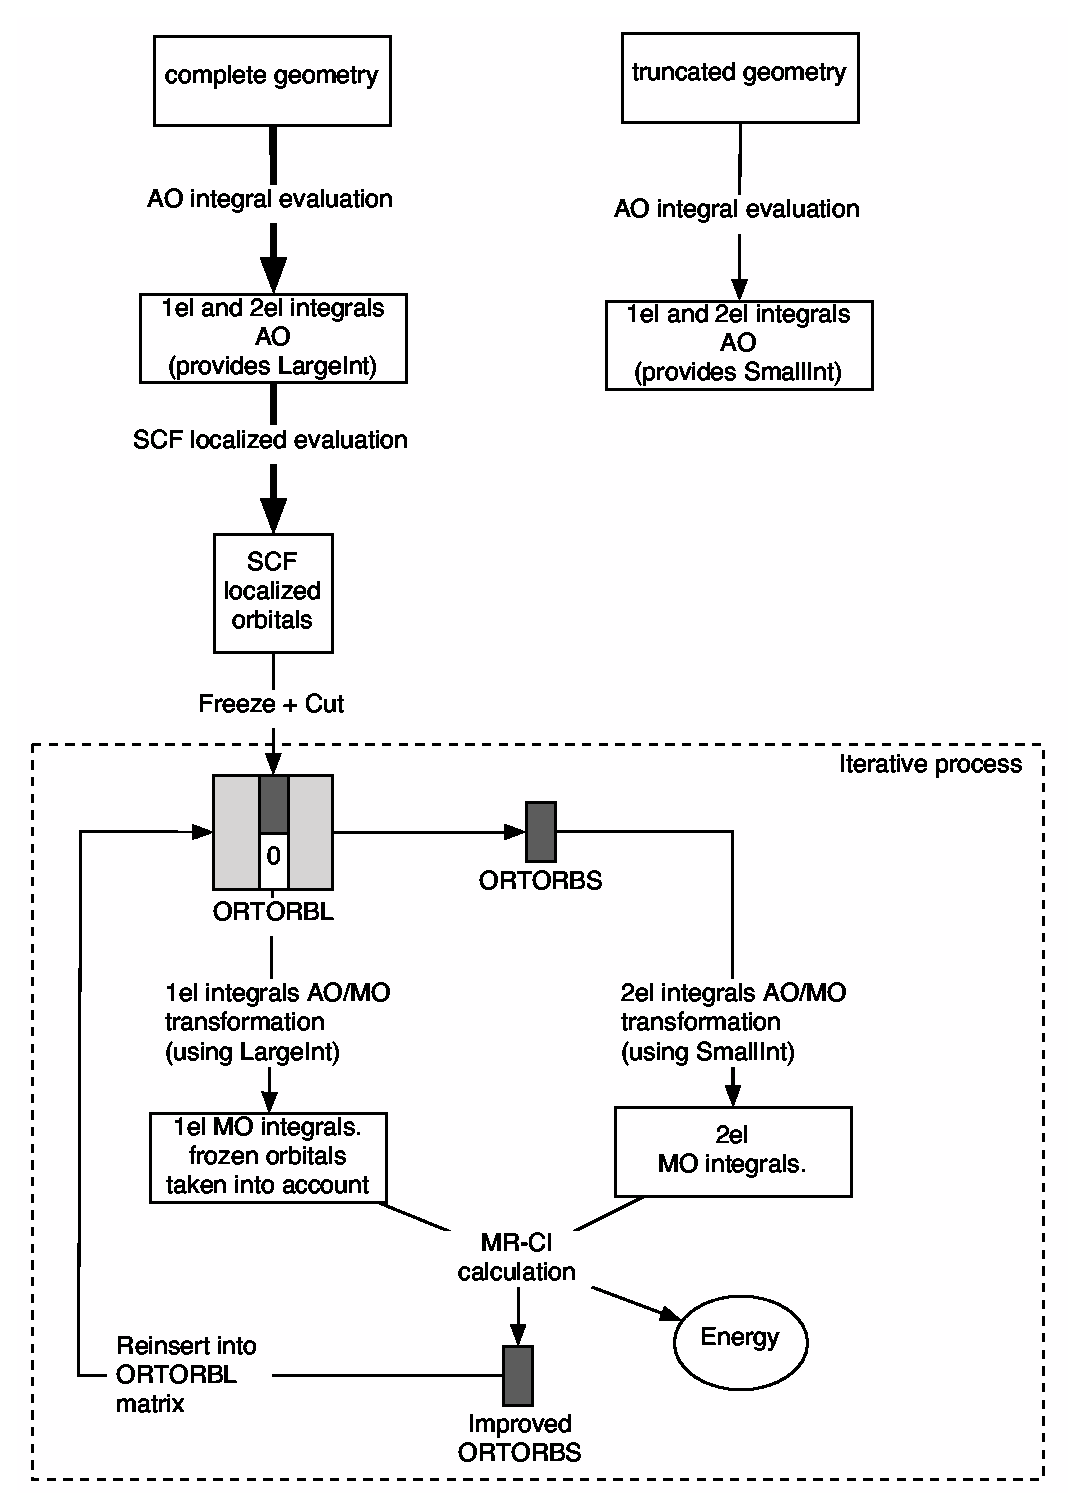
\includegraphics[width=13cm,keepaspectratio]{02_localization/images/logical-scheme-gimped.eps}
\caption{\footnotesize Logical steps (arrows) and obtained entities (boxes) for the
presented procedure. Thick lines denote steps that still depend on two
electron AO integrals on the complete geometry of the system
} \label{fig:logical-scheme}
\end{center}
\end{figure}


These steps describe in more detail the process labeled 
as ``SCF localized evaluation'' in Fig.~\ref{fig:logical-scheme}. The result
is a set of orthogonal localized SCF orbitals.

Thanks to the localization procedure, each localized SCF orbital is mainly
described on a reduced set of atomic basis functions. These orbitals can now
be tagged on two degrees of freedom: the freezing selection of certain
localized SCF orbitals, and the cut of a set of atomic basis functions for
the non-frozen orbitals. The latter is realized by setting to zero the
coefficients that express the non-frozen orbitals on the cut atomic basis
set. This operation effectively projects the non-frozen MO in a reduced
atomic basis space, and the approximation is good as long as the target
coefficients are already close to zero due to the localization.

The large MO matrix (refer to the detailed pictorial representation in
Fig.~\ref{fig:matrix}) holds molecular orbitals that are no longer
orthonormal, although it must be pointed out that the overlap between them
is small. A hierarchical orthonormalization is performed to obtain an
orthonormal set: first the non-frozen orbitals among themselves, then the
frozen occupied orbitals with respect the non-frozen, and finally the frozen
virtual orbitals. Thanks to the hierarchical procedure, the coefficients
that have been set to zero remain unchanged. This is important in order to
keep the non-frozen orbitals inside a smaller AO space.

Finally, a smaller matrix is obtained by extracting the submatrix
of the non-frozen orbitals against the smaller, non-cut atomic set.
The final result of this process are two matrixes, named ORTORBL and
ORTORBS, which hold the molecular orbitals as described, respectively for
the large and the small system (complete system and truncated one).

After an AO/MO integral transformation, the optimization chain is now fed
with two-electron MO integrals (which derive only from orbitals
that are not frozen) and with the modified one-electron integrals that keep
into account the two-electron contribution from the frozen set. 

At each iteration, the procedure works as follows:
\begin{itemize}
\item calculate an improved density matrix using a Super-CI
optimization that preserves orbitals locality. This process is
done only on the restricted subset of non-frozen orbitals, and only on the
available framework of non-cut atoms, leading to an improved set
of orbitals (improved ORTORBS)
\item reinsert the improved orbitals inside the frozen framework, thus creating
an improved ORTORBL large matrix
\item recreate a new set of MO two-electron integrals, transforming the AO integrals
from the truncated system using the improved ORTORBS orbitals
\item recreate a new set of MO one-electron integrals with the improved ORTORBL set
and the complete system
\item iterate until convergence is reached (no change in the energy within a
given level of approximation)
\end{itemize}

\input{02_localization/04_freeze_and_cut_implementation}
\pagebreak
\section{Evaluations}
\subsection{(7Z)-13 ammoniotridec-7-enoate}

The first test case presented is relative to (7Z)-13 ammoniotridec-7-enoate, an
aminoacid zwitterion specifically designed to test the response of the
method to charge interactions (see Fig. \ref{fig:7Z-molecule}). The rigid
rotational behavior around the central double bond has been evaluated,
describing the absolute CAS+Single excitations (CAS+S) energy curves without
geometry relaxation with respect to the torsional dihedral angle. 

\begin{figure}[ht]
\begin{center}
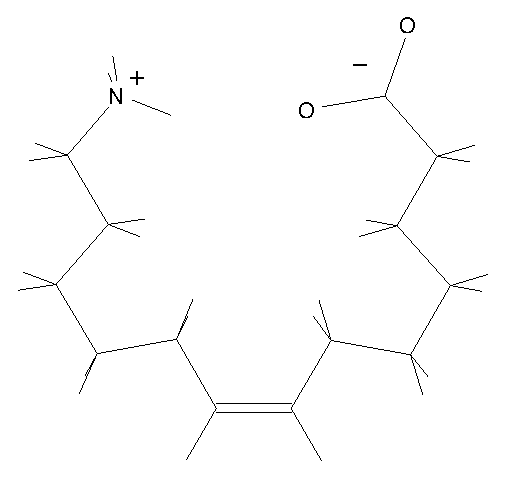
\includegraphics[width=7cm,keepaspectratio]{02_localization/images/7Z-molecule.eps}
\caption{\footnotesize The (7Z)-13 ammoniotridec-7-enoate molecule. The cis-trans rigid
interconversion around the central double bond has been performed to test
the presented method. }
\label{fig:7Z-molecule}
\end{center}
\end{figure}



All the calculations have been performed by using ANO basis sets.
A minimal basis set ANO-1\cite{tca-77-291-1990} with
$2s1p$ contraction for C,N,O and $1s$ contraction for hydrogen atoms was
used.  The interatomic distances (in $\mbox{{\AA}ngstrom}$) are
r(C-C)=1.450, r(C=C)=1.335, r(C-H)=1.089, r(C-N)=1.440, r(N-H)=1.008,
r(C-O)=1.400. The angles are 109.5 degrees except for the C=C group and the
COO$^{-}$ group, where angles of 120 degrees have been used.
The dihedral angles were adjusted to obtain the cis and trans molecular
skeleton lying completely on the plane.

The CAS space selection consists of 2 electrons in 2 orbitals (C-C $\pi$
and $\pi^{*}$). This selection has been chosen to keep into account the
main correlative effects due to the rotation around the central
carbon-carbon double bond.

It must be stressed that, due to geometrical proximity, the interaction
between the charged groups affects the rotational behavior, and its
contribution must be kept into account.  For this reason, the two terminal groups
cannot be simply removed and replaced by hydrogen atoms.
As a comparison example, Fig.~\ref{fig:7Z-nocharges} shows the
behavior obtained by removing these groups and replacing them with
hydrogens. 

\begin{figure}[t]
\begin{center}
\includegraphics[width=8cm,angle=270]{02_localization/images/7Z-nocharges.eps}
\caption{\footnotesize A comparison of the CAS+S energy curves between the zwitterionic
(7Z)-13 ammoniotridec-7-enoate (solid line) and the (6Z)-dodec-6-ene, a
molecule obtained by replacing the charged NH$_{3}$ and COO$^{-}$ groups
with hydrogen atoms, dashed line.  A common zero in the energy scale of the
plot has been obtained taking the trans form as zero of the energy.  }
\label{fig:7Z-nocharges}
\end{center}
\end{figure}


Using the Freeze-and-Cut technique, the evaluation performed on a
small system reproduces the expected behavior: the freezing preserves the
electronic contribution of the groups, and the cut allows to work with a
reduced molecular system.

\begin{figure}[h!]
\begin{center}
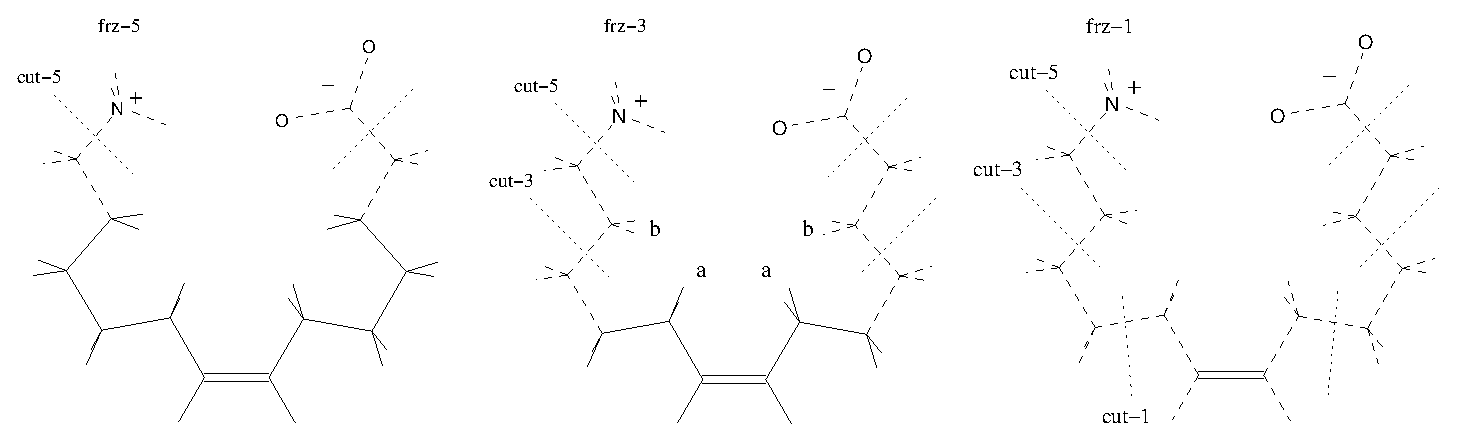
\includegraphics[width=12cm,keepaspectratio]{02_localization/images/7Z-frzcut-schema.eps}
\caption{\footnotesize (7Z)-13 ammoniotridec-7-enoate. Localized orbitals expressed on
atoms of the dashed line framework are frozen. Orbitals expressed on atoms
of the solid line framework are not frozen. Dotted lines depict the
cut seam. The cut is always performed on both chains, from ``cut-5'' (only
the charged groups are removed from the molecule, both left and right) to
``cut-1'' (maximal cut selection, only the central double bond and left and
right -CH$_{2}$- spacers are preserved). The ``a'' and ``b'' symbols in frz-3 picture
are labels for interesting hydrogen atoms. See text for details.  }
\label{fig:7Z-frzcut-schema}
\end{center}
\end{figure}


Different freeze and cut strategies have been chosen in order to evaluate
the behavior of our technique with respect to these selections.
Three freezing levels, labeled ``frz-1,'' ``frz-3'' and ``frz-5'' have been
defined (Fig. \ref{fig:7Z-frzcut-schema}), and also a ``nofrz'' level
where no freezing has been performed.  The $1s$ core atomic orbitals for heavy
atoms have been frozen at SCF level regardless of the atom positions.

The cut strategy follows the freezing strategy. Four cut thresholds have
been chosen, with labels ``cut-1,'' ``cut-3,'' ``cut-5'' and ``nocut,''
following the freezing choice, but preserving a -CH$_2$-
spacer between the last not frozen orbital and the first cutout atom.

The analysis performed at 0 (cis) and 180 (trans) degrees and their
difference are presented in Tab. \ref{tbl:7Z-cis-trans-diff}

\begin{center}
\begin{threeparttable}
\begin{tabular}{lcccc}
\hline
    		&		nofrz			&	frz-5				&	frz-3				&	frz-1	\\	
\hline
			&	\multicolumn{4}{c}{Cis} \\
nocut		&	-709.483006     	&	-709.482889     	&	-709.482281     	&	-709.465687      \\
cut-5		&						&	-709.373507  		&   -709.479395  		&	-709.465638      \\
cut-3		&						&						&	-709.218388     	&	-709.460918      \\
cut-1		&						&						&						&	-709.357068    	 \\
			&	\multicolumn{4}{c}{Trans} \\
nocut		&	-709.388878     	&	-709.388760     	&	-709.388156     	&	-709.371500      \\
cut-5		&						&	-709.279814  		&   -709.385430  		&	-709.371437      \\
cut-3		&						&						&	-709.123318     	&	-709.366578      \\
cut-1		&						&						&						&	-709.258750    	 \\
			&	\multicolumn{4}{c}{Diff} \\
nocut		&	59.0267         	&	59.0272         	&	59.0251         	&	59.0640        	 \\
cut-5		&						&	58.7538         	&	58.9248         	&	59.0725          \\
cut-3		&						&						&	59.6173         	&	59.1598          \\
cut-1		&						&						&						&	61.6542        	 \\
\hline
\end{tabular}
\caption{\footnotesize CAS+S absolute energies (Hartree) and energy
difference (kcal/mol) between (7Z)-13 ammoniotridec-7-enoate cis and trans
structure, with respect to different freeze and cut strategies.}
\label{tbl:7Z-cis-trans-diff}
\end{threeparttable}
\end{center}


It can be seen that the cut technique produces energy differences between
cis and trans that are comparable to the reference value obtained with no
cut and freeze.

A different behavior can be evaluated for the difference between the 0 degrees
form and the 90 degrees form (Tab. \ref{tbl:7Z-diff-cis-90})

\begin{center}
\begin{threeparttable}
\begin{tabular}{lcccc}
\hline
			&		nofrz			&	frz-5				&	frz-3				&	frz-1	\\
\hline
nocut		&	130.4145        	&	130.4953        	&	131.2643        	&	167.4817         \\
cut-5		&						&	130.1703        	&	131.1572        	&	167.5065         \\
cut-3		&						&						&	130.8074        	&	168.4879         \\
cut-1		&						&						&						&	171.2689       	\\
\hline
\end{tabular}
\caption{\footnotesize CAS+S energy difference (kcal/mol) between the (7Z)-13
ammoniotridec-7-enoate cis and the 90 degrees twisted structure with respect
to different freeze and cut strategies.}
\label{tbl:7Z-diff-cis-90}
\end{threeparttable}
\end{center}


The frz-1 selection presents a large deviation from the expected value. This
arises from the fact that the SCF at 90 degrees evaluates very poorly the
orbitals involved (directly or indirectly) in the bond breaking. 

This leads to an initial bad description of the orbitals, which are frozen
at this poor quality level. As a consequence, the optimization guess is
affected by this initial description. By relaxing the freeze selection,
these orbitals are allowed to improve in the subsequent iterative process,
thus drastically reducing the incorrect behavior. In the case of frz-1
strategy, however, the effects are too pronounced to be smoothed out.

\begin{figure}[h!]
\begin{center}
\includegraphics[width=8cm,keepaspectratio,angle=270]{02_localization/images/7Z-frz-1.eps}
\caption{\footnotesize CAS+S energy curves (Hartree) for the cis-trans rigid
interconversion of the (7Z)-13 ammoniotridec-7-enoate with different 
cut strategies and frz-1 freeze strategy. The reference (solid black line)
is evaluated on the complete molecular system with no frozen orbitals except
the $1s$ core orbital for heavy atoms. frz-1/nocut curve (dotted line,
$\Box$ symbol) and frz-1/cut-5 (short dash line, $\times$ symbol) appear as
superposed on the drawing scale. The other curves are frz-1/cut-3 (long
dash line, $\bigcirc$ symbol) and frz-1/cut-1 (dot-dash line, $\Diamond$
symbol).  }
\label{fig:7Z-frz-1}
\end{center}
\end{figure}



This is of particular evidence in the curve diagrams depicted in
Fig.~\ref{fig:7Z-frz-1}: the solid line is the nofrz/nocut reference,
obtained by interpolating points from 0 to 180 (step 10 degrees) with a
cubic spline curve. The other curves represent the incorrect behavior of
frz-1 with cut strategies cut-1, cut-3, cut-5 and nocut (these last two
curves are superposed).  Each point has been generated using as a starting
guess the converged orbitals from the previous point on the complete AO
space (the ORTORBL matrix at convergence). Depending on the guess (70 or 110
degrees), two different curves can be obtained, giving a spike at 90
degrees.  This reflects the dependence on the SCF solution, which affects
the frozen orbital framework. It is however important to note that these
curves are still parallel to the reference curve when far from the 90
degrees region. 

As can be seen from Fig. \ref{fig:7Z-frz-3}, this incorrect behavior is
drastically reduced by going from frz-1 to frz-3.

\begin{figure}[ht]
\begin{center}
\includegraphics[width=8cm,angle=270]{02_localization/images/7Z-frz-3.eps}
\caption{\footnotesize CAS+S energy curves (Hartree) for the cis-trans rigid
interconversion of the (7Z)-13 ammoniotridec-7-enoate with different 
cut strategies and frz-3 freeze strategy. The reference (solid black line,
see caption of Fig.\ref{fig:7Z-frz-1} for details),
frz-3/nocut curve (dotted line, $\Box$ symbol) and frz-3/cut-5 (short
dash line, $\times$ symbol) appear nearly superposed on the drawing
scale. The other curve is frz-3/cut-3 (long dash line, $\bigcirc$ symbol).
}
\label{fig:7Z-frz-3}
\end{center}
\end{figure}


The curves are nearly parallel to the reference, but with a strong energy
shift between cut-3 and cut-5.
This difference is principally due to the four non-frozen C-H bonds (marked
with the ``a'' labels in Fig. \ref{fig:7Z-frzcut-schema}): they are
described by hydrogen atoms (marked with the ``b'' labels)
that have been cut out from the small system in the cut-3 analysis. This
results in a shift in absolute energies, but does not affect the relative
behavior.

Treating the same cut-3 system, but also adding the ``b'' hydrogen atoms
gives CAS+S energies in better accord with the frz-3/cut-5 values,
providing nearly half of the gap between frz-3/cut-3 and frz-3/cut-5.
%(see Tab. \ref{tbl:7Z-trend}).
\begin{center}
\begin{threeparttable}
\begin{tabular*}{0.80\textwidth}{l@{\hspace*{10mm}}cccc}
\hline
					&	cis			&	trans			&	diff   \\
\hline
frz-3/cut-5			&	-709.479395      	&	-709.385430        	&  58.9248 \\
frz-3/cut-3+H$_{\mbox{b}}$	&	-709.374870			&	-709.280646       	&  59.0873 \\
frz-3/cut-3			&	-709.218388			&	-709.123318			&  59.6173 \\
\hline
\end{tabular*}
\caption{\footnotesize CAS+S absolute energies (Hartree) and energy
difference (kcal/mol) between (7Z)-13 ammoniotridec-7-enoate cis and trans
for frz-3/cut-3, frz-3/cut-5 and the intermediate frz-3/cut-3+H$_b$, where
hydrogens labeled ``b'' in Fig.  \ref{fig:7Z-frzcut-schema}
have been preserved for the cut-3 strategy.}
\label{tbl:7Z-trend}
\end{threeparttable}
\end{center}

This confirms the importance of these four hydrogens for the evaluation
of the absolute energy, but the relative behavior is unaffected.
The same effect arises in all the diagonal values of the absolute energy
tables, where a similar situation happens due to the proximity of
the cut seam to the non-frozen orbitals.

The frz-3 selection has also been studied with a larger CAS space.
This has been obtained by enriching the previous space with the C-C $\sigma$
and $\sigma^{*}$ orbitals, thus leading to a 4 electron in 4 orbitals space.
\begin{figure}[h!]
\begin{center}
\includegraphics[width=78mm,angle=270]{02_localization/images/7Z-frz-3-cas44.eps}
\caption{\footnotesize CAS+S energy curves (Hartree) for the cis-trans rigid
interconversion of the (7Z)-13 ammoniotridec-7-enoate with an extended CAS
defined as 4 electrons in 4 orbitals, with different cut strategies for the
frz-3 freeze strategy. The reference (solid black line, see caption of
Fig.\ref{fig:7Z-frz-1} for details), frz-3/nocut curve (dotted line,
$\Box$ symbol) and frz-3/cut-5 (short dash line, $\times$ symbol) appear
nearly superposed on the drawing scale. The other curve is frz-3/cut-3 (long
dash line, $\bigcirc$ symbol).
}
\label{fig:7Z-frz-3-cas44}
\end{center}
\end{figure}


The evaluation has been performed at 90 degrees and from 0 to 180 degrees
with a step of 20 degrees, interpolating the points with a cubic spline curve.

As can be seen from Fig. \ref{fig:7Z-frz-3-cas44} the same correct
behavior is obtained, the only difference being the shift of the energy due
to the larger CAS space. The relative energy for the frz-3/cut-3 is, for
example, 59.6149 kcal/mol. This value is in a very good accord with the one
obtained using the CAS 2/2 space, 59.6173 kcal/mol.

Fig. \ref{fig:7Z-frz-5} finally depicts the results for frz-5 strategy with the
CAS 2/2 space, where frz-5/cut-5 curve lays higher in energy but still
parallel to the reference curve, and the frz-5/nocut curve nearly superposed
to the reference. 
\begin{figure}[ht]
\begin{center}
\includegraphics[width=8cm,angle=270]{02_localization/images/7Z-frz-5.eps}
\caption{\footnotesize CAS+S energy curves (Hartree) for the cis-trans rigid
interconversion of the (7Z)-13 ammoniotridec-7-enoate with different cut
strategies and frz-5 freeze strategy. The reference (solid black line, see
caption of Fig.\ref{fig:7Z-frz-1} for details) and frz-5/nocut curve
(dotted line, $\Box$ symbol) appear as superposed on the drawing scale.  The
other curve is frz-5/cut-5 (short dash line, $\times$ symbol) 
}
\label{fig:7Z-frz-5}
\end{center}
\end{figure}


Fig.\ref{fig:7Z-orbitals} shows the optimized $\pi$ orbital for the cis
molecule with different cut strategies at frz-1 level of freeze. The plots
have been realized with the Molden program\cite{molden-site} with a contour
factor of 0.002. We can note that the cut-5 strategy does not change the
orbital in a significant way, due to the graphically negligible expression
of the orthogonalization tail of the orbital on the removed fragments.  The
cut-3 and cut-1 strategies show instead the confinement of the optimized
orbital inside the group of atoms on which the projection was performed.
The small lobes for the $\pi$ description are removed by the cut procedure,
and the optimization preserves the locality imposed by the method.

%\begin{wrapfigure}{l}{65mm}
%\vspace{3mm}
%\end{wrapfigure}
\begin{center}
\begin{figure}[h!]
\begin{center}
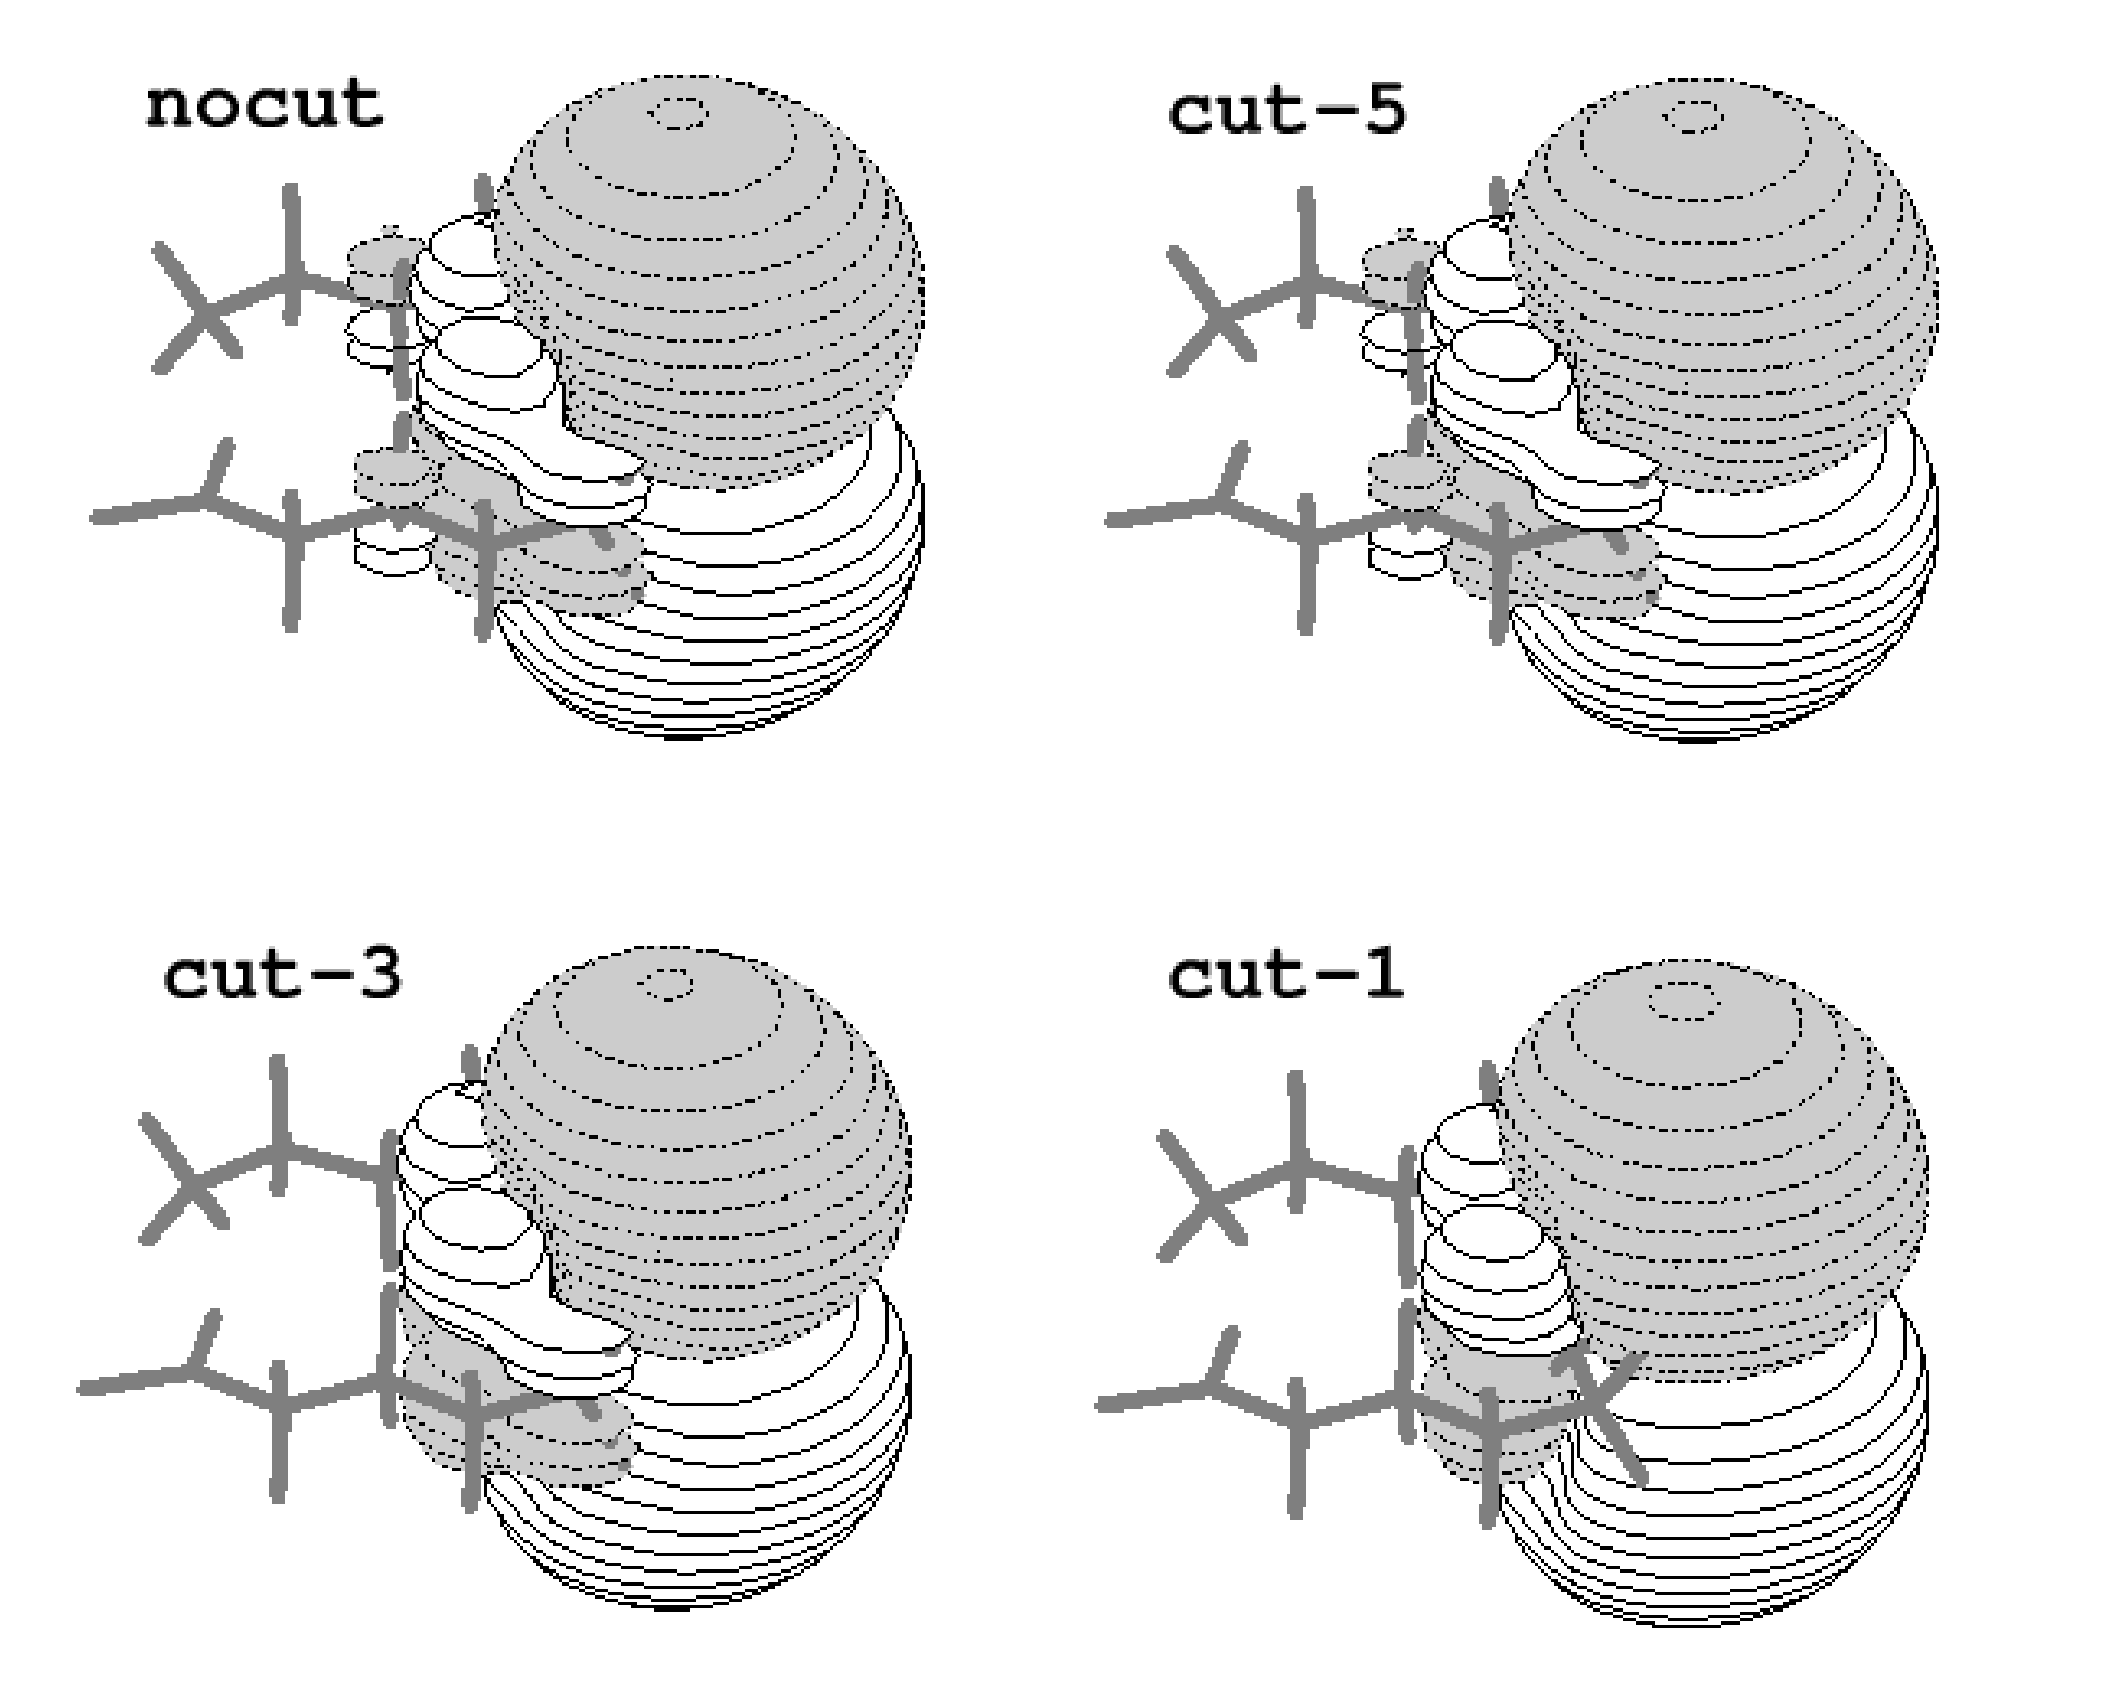
\includegraphics[width=72mm,keepaspectratio]{02_localization/images/7Z-orbitals.eps}
\caption{\footnotesize The $\pi$ orbital representation with respect to different cut strategies at frz-1
freeze strategy. }
\label{fig:7Z-orbitals}
\end{center}
\end{figure}
\end{center}



The improvements in timings are presented as an example in Tab. \ref{tbl:timings},
applied to the (7Z)-13 ammoniotridec-7-enoate with the CAS 2/2 space.

As can be seen, performing the integral evaluation on the reduced
system is a lightweight process.
Nocut evaluations have a value of zero for the reduced system. The integral
evaluation on the complete system can be used in this case, saving the cost
of a new evaluation.

The remaining steps are quite fast, but the best compromise between result
quality and time is for the frz-3/cut-3 evaluation.
In this case a reduction of the time needed to perform the optimization is
counterbalanced by the need of an integral evaluation on the small system,
but the difference between the frz-3/cut-3 and the frz-3/nocut becomes
dramatic when working on systems larger than the presented ones, which are
the final targets of this technique.

\begin{center}
\begin{table}[ht]
\footnotesize
\begin{center}
\begin{tabular}{lcccccc}
\hline
				&	seward-large	&	seward-small		&	large	& small	&	CAS+S	&	total \\
\hline
nofrz/nocut		&	1009			&			0			&	50		&	39		&	1062	&	2160 \\
frz-5/nocut		&	1009			&			0			&	50		&	19		&	355		&	1433 \\
frz-5/cut-5		&	1009			&			433			&	50		&	6		&	225		&	1723 \\
frz-3/nocut		&	1009			&			0			&	50		&	7		&	184		&	1250 \\
frz-3/cut-3		&	1009			&			100			&	50		&	1		&	99		&	1259 \\
frz-1/nocut		&	1009			&			0			&	50		&	2		&	43		&	1104 \\
frz-1/cut-1		&	1009			&			8			&	50		&	0		&	18		&	1085 \\
\hline
\end{tabular}
\end{center}
\caption{\footnotesize Timings (in seconds) for evaluations performed on (7Z)-13
ammoniotridec-7-enoate, against different freeze and cut strategies. Test
performed on Intel dual Xeon 2.8 GHz 2 GB RAM. ``seward-large'' and ``seward-small''
are the timings for the AO integral evaluation. ``large'' and ``small'' columns
represents the timings needed for the creation of the transformed integrals
which will seed the first iteration. ``CAS+S'' column reports the timings for
the complete iterative procedure up to the convergence.}
\label{tbl:timings}
\end{table}
\end{center}



\subsection{C$_{13}$ polyenal}

A second test was performed on the highly conjugated C$_{13}$ polyenal

\begin{center}
\begin{figure}[ht]
\begin{center}
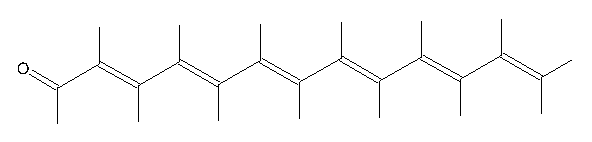
\includegraphics[width=10cm]{02_localization/images/C13-molecule.eps}
\end{center}
\caption{\footnotesize The C$_{13}$ transoid polyenal molecule. }
\label{fig:C13-molecule}
\end{figure}
\end{center}

\vspace{-5mm}
Applications of the localization technique on polyenals have been performed
\cite{mp-101-1389-2003,cpl-372-22-2003,ijqc-97-688-2004}.
This class of molecules is of particular interest due to their role in
photobiology as chromophores \cite{jacs-118-7790-1996}.
Moreover, they are excellent model systems for studying
the interaction between the $\pi$ system of the carbonyl group and the
$\pi$ system of the unsaturated chain \cite{tetrahedron-34-3591-1978}. 

The cisoid-transoid energy difference for the aldehydic group has been
studied, by rotating by 180 degrees the C-C single bond. This evaluation
should be very weakly affected by the length of the polyene chain. The
distances (in $\mbox{{\AA}ngstrom}$) are r(C=O)=1.220, r(C-C)=1.450,
r(C=C)=1.350, r(C-H)=1.100.  All angles are 120 degrees.  The cut and freeze
denomination follows the analogy with shorter chain polyenals, as depicted
in Fig.~\ref{fig:C13-selection}.

\begin{center}
\begin{figure}[h!]
\begin{center}
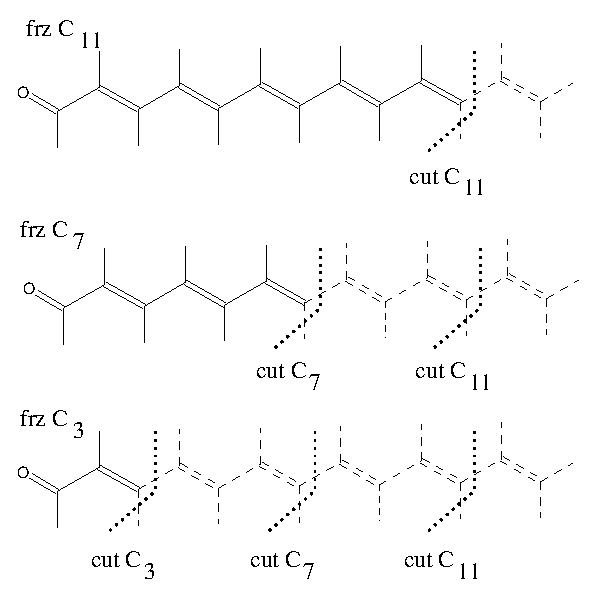
\includegraphics[width=8cm,keepaspectratio]{02_localization/images/C13-selection.eps}
\end{center}
\caption{\footnotesize C$_{13}$ polyenal molecule. Freeze and cut strategy
and labels follow the analogy with shorter chain polyenals. Localized
orbitals expressed on atoms of the dashed line framework are frozen.
Dotted lines depict the cut seam.  }
\label{fig:C13-selection}
\end{figure}
\end{center}


Two basis sets have been used: a minimal basis of type ANO-1 with $2s1p$
contraction for C and O, and a $1s$ contraction for hydrogen atoms
(hereafter named ANO-small), and a larger one ANO-1 with $3s2p$ contraction
for C and O, and a $2s$ contraction for hydrogens (ANO-large). As in the
previous case, the $1s$ core orbitals for carbon and oxygen atoms have been
frozen regardless of the freezing strategy.

Two CAS spaces have been considered. The first one, named CAS-A, contains
two electrons in the $\pi$/$\pi^{*}$ orbitals of the carbonyl group. The
second active space, named CAS-B, is defined as the previous one, further
extended with the inclusion of two additional electrons and the
$\pi$/$\pi^{*}$ orbitals from the double bond near the carbonyl. 

A preliminary evaluation with the ANO-small basis set and the CAS-A active
space has been performed on smaller polyenals, obtained by replacing the
removed part of the molecule with a hydrogen atom. The obtained results are
presented in Tab.~\ref{tbl:smaller-poly}.

\begin{center}
\begin{table}[ht]
\begin{center}
\footnotesize
\begin{tabular*}{0.75\textwidth}{l@{\hspace*{40mm}}ccc}
\hline
      	&    cisoid	&   transoid	  & diff	 \\
\hline
C$_{3}$ 	& -190.457653  	&	-190.460042   &	1.4981    \\
C$_{7}$ 	& -343.919126  	&	-343.921129   &	1.2563    \\
C$_{11}$	& -497.381057   &	-497.383042   &	1.2446    \\
C$_{13}$	& -574.112029   &	-574.114015   & 1.2453    \\
\hline
\end{tabular*}
\end{center}
\caption{\footnotesize CAS+S energy (Hartree) and difference (kcal/mol) between cisoid and
transoid complete structure for smaller polyenals, using the CAS-A active
space and the ANO-small basis set.}
\label{tbl:smaller-poly}
\end{table}
\end{center}


Tab. \ref{tbl:C13-cis-trans-diff} shows the absolute values for the CAS-A
with ANO-small basis set. Values are well reproduced, except when the cut is
near the frozen/non-frozen seam. This confirms the preceding statement
about this behavior. Also, the relative energies behave as expected. Again,
we can see that in the most pronounced Freeze-and-Cut strategy the results
are poor even in the relative energy.

Evaluation with the larger CAS-B (Tab.~\ref{tbl:C13-cis-trans-diff-casb})
and with the larger ANO-large basis set
(Tab.~\ref{tbl:C13-cis-trans-diff-ano-large}) show the same behavior.

Finally Fig. \ref{fig:C13-orbitals} shows the $\pi$ orbital for different cut
strategies, on the cisoid structure. Again, the Molden contour factor was
0.002, and the same behavior reported for the (7Z)-13 ammoniotridec-7-enoate
can be appreciated.  The cut-C11 strategy does not change the orbital in a
significant way, due to the graphically negligible expression of the
orthogonalization tail of the orbital on the removed part.  The other
strategies progressively restrict the orbital into the preserved part of
the polyenal.

\begin{center}
\begin{table}[ht]
\footnotesize
\begin{center}
\begin{tabular}{lcccc}
\hline                                                      
        &    nofrz       &    frz C$_{11}$      &   frz C$_{7}$        &   frz
C$_{3}$      \\
\hline                                                      
			&	\multicolumn{4}{c}{Cisoid} \\
nocut	&  -574.112029   &  -574.112025    &  -574.111981   & -574.110699   \\
cut C$_{11}$	&             	 &  -573.831612    &  -574.110383   & -574.110600   \\
cut C$_{7}$	&             	 &                 &  -573.826403   & -574.108770   \\
cut C$_{3}$	&             	 &             	  &                & -573.837474  	\\
			&	\multicolumn{4}{c}{Transoid} \\
nocut		&	-574.114015  	&	-574.114009  	&	-574.113945  	& -574.112686   \\
cut C$_{11}$&	             	&	-573.833584  	&	-574.112346  	& -574.112589   \\
cut C$_{7}$	&					&					&	-573.828399  	& -574.110797   \\
cut C$_{3}$	&					&					&					& -573.838137  	\\
			&	\multicolumn{4}{c}{Diff} \\
nocut			& 1.2453    &	1.2438    	&	1.2367    	&	1.2461    \\
cut C$_{11}$	&			&  	1.2367    	&	1.2314    	&	1.2474    \\
cut C$_{7}$		&			&				&  	1.2513    	&	1.2708    \\
cut C$_{3}$		&			&				&				&  	0.4161    \\
\hline
\end{tabular}
\end{center}
\caption{\footnotesize CAS+S absolute energies (Hartree) and energy
difference (kcal/mol) between cisoid and transoid C$_{13}$ polyenal using
the CAS-A active space and the ANO-small basis set, with respect to
different freeze and cut strategies.}
\label{tbl:C13-cis-trans-diff}
\end{table}
\end{center}

\begin{center}
\begin{table}[!ht]
\footnotesize
\begin{center}
\begin{tabular}{lcccc}
\hline
       &    nofrz       &    frz C$_{11}$      &   frz C$_{7}$        &   frz
C$_{3}$      \\
\hline                                                      
			&	\multicolumn{4}{c}{Cisoid} \\
nocut		&  -574.173041   &  -574.172995    	&  -574.172423   & -574.158115   \\
cut C$_{11}$&             	 &  -573.892623    	&  -574.170812   & -574.157975   \\
cut C$_{7}$	&             	 &                	&  -573.887517   & -574.156091   \\
cut C$_{3}$	&             	 &					&                & -573.889043  	\\
			&	\multicolumn{4}{c}{Transoid} \\
nocut		&	-574.174560  	&	-574.174521  	&	-574.174006  	& -574.160153   \\
cut C$_{11}$&	             	&	-573.894131  	&	-574.172393  	& -574.160015   \\
cut C$_{7}$	&					&					&	-573.889012  	& -574.158166   \\
cut C$_{3}$	&					&					&					& -573.888923  	\\
			&	\multicolumn{4}{c}{Diff} \\
nocut			& 0.9522    &	0.9567    	&	0.9919    	&	1.2776    \\
cut C$_{11}$	&			&  	0.9459    	&	0.9916    	&	1.2795    \\
cut C$_{7}$		&			&				&  	0.9378    	&	1.3015    \\
cut C$_{3}$		&			&				&				&  -0.0756    \\
\hline
\end{tabular}
\end{center}
\caption{\footnotesize CAS+S absolute energies and energy difference
(kcal/mol) between cisoid and transoid C$_{13}$ polyenal using the CAS-B
active space and the ANO-small basis set with respect to different freeze
and cut strategies.}
\label{tbl:C13-cis-trans-diff-casb}
\end{table}
\end{center}


\begin{center}
\begin{table}[!ht]
\footnotesize
\begin{center}
\begin{tabular}{lcccc}
\hline                                                      
        &    nofrz       &    frz C$_{11}$      &   frz C$_{7}$        &   frz C$_{3}$      \\
\hline                                                      
			&	\multicolumn{4}{c}{Cisoid} \\
nocut		&  -575.112195   &  -575.112194    	&  -575.112159   & -575.111082   \\
cut C$_{11}$&             	 &  -574.845588    	&  -575.108852   & -575.110774   \\
cut C$_{7}$	&             	 &                	&  -574.833700   & -575.106924   \\
cut C$_{3}$	&             	 &					&                & -574.850622  	\\
			&	\multicolumn{4}{c}{Transoid} \\
nocut		&	-575.115498  	&	-575.115500  	&	-575.115451  	& -575.114549   \\
cut C$_{11}$&	             	&	-574.848881  	&	-575.112168  	& -575.114263   \\
cut C$_{7}$	&					&					&	-574.837108  	& -575.110644   \\
cut C$_{3}$	&					&					&					& -574.849650  	\\
			&	\multicolumn{4}{c}{Diff} \\
nocut			& 2.0716    &	2.0738    	&	2.0644    	&	2.1742    \\
cut C$_{11}$	&			&  	2.0652     	&	2.0792    	&	2.1877    \\
cut C$_{7}$		&			&				&  	2.1369    	&	2.3328    \\
cut C$_{3}$		&			&				&				&  -0.6100    \\
\hline
\end{tabular}
\end{center}
\caption{\footnotesize CAS+S absolute energies and energy difference
(kcal/mol) between cisoid and transoid C$_{13}$ polyenal using the CAS-A
active space and the ANO-large basis set with respect to different freeze
and cut strategies.}
\label{tbl:C13-cis-trans-diff-ano-large}
\end{table}
\end{center}


\begin{figure}[!ht]
\begin{center}
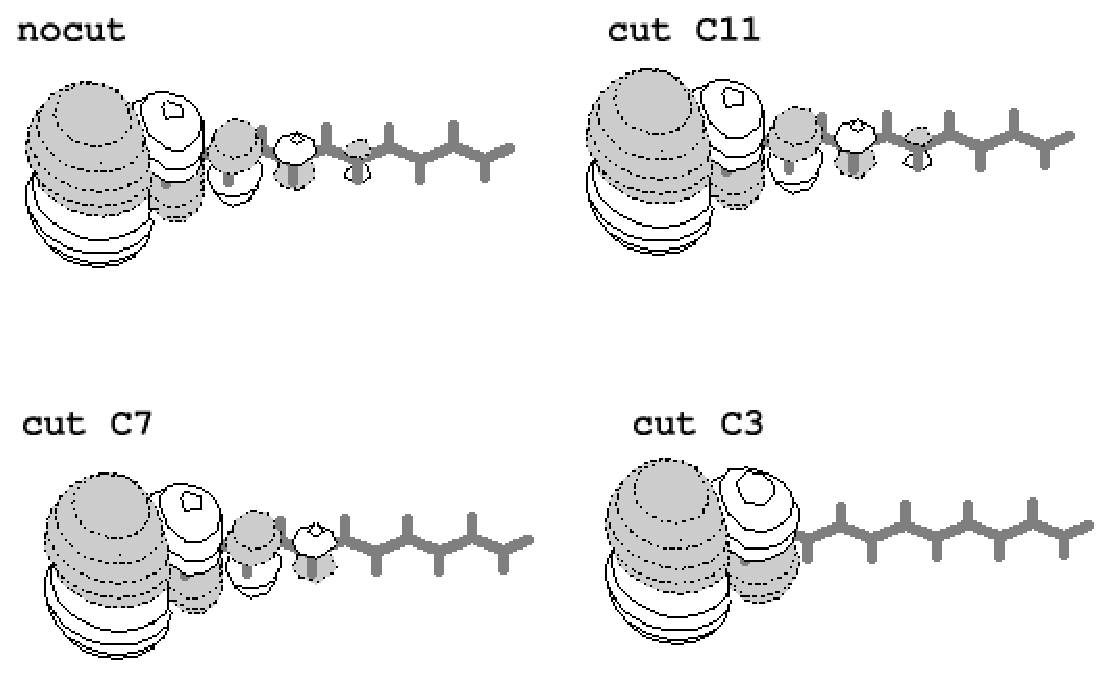
\includegraphics[width=8cm]{02_localization/images/C13-orbitals.eps}
\end{center}
\caption{\footnotesize The $\pi$ orbital for the C$_{13}$ cisoid polyenal with respect to
different cut strategies at frz-C$_{3}$ freeze strategy. The Molden contour factor for
the plot is 0.002. The progressive neglect of the orbital expression on
cut atoms can be appreciated.
}
\label{fig:C13-orbitals}
\end{figure}



\clearpage

\newpage
\subsection{Acetone + Water}

To gain better insights about the sensibility of the technique with respect
to the basis set, another test has been performed with the acetone molecule
surrounded by six water molecules. Two molecules are directly coordinated to
the carbonyl oxygen, while the remaining four coordinate the first
two molecules.

\begin{figure}[ht]
\begin{center}
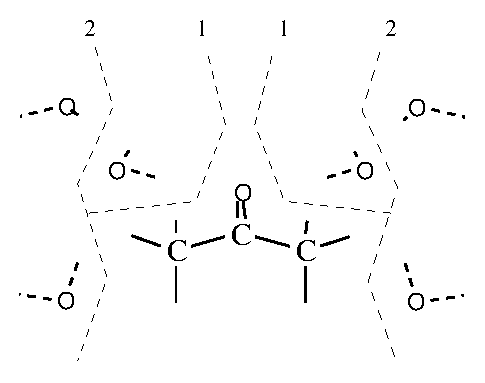
\includegraphics[width=10cm,keepaspectratio]{02_localization/images/acetone-water-frzcut-schema.eps}
\caption{\footnotesize Scheme for freeze and cut of the acetone + 6 H$_2$O
system. Surrounding water molecules have been completely frozen, and two cut
seams have been chosen to remove these molecules completely (seam ``1'') or
partially (seam ``2''). }
\label{fig:acetone-water-frzcut-schema}
\end{center}
\end{figure}

\vspace{-5mm}
The freeze and cut scheme focuses on a full freezing of the water molecules.
Two cut levels have been implemented: the first level completely removes the
water system, and the second level preserves only the two carbonyl-coordinated molecules.

The active space included five orbitals (the oxygen $n_y$ lone pair, and
carbonyl $\pi$, $\pi^{*}$, $\sigma$ and $\sigma^{*}$ orbitals) with six
active electrons. A state average optimization involving the ground state
and the $n \rightarrow \pi^{*}$ has been performed to evaluate this vertical
transition energy.

Two ANO-1 basis sets contractions have been used: the minimal set
C,O[$2s1p$], H[$1s$], hereafter called Bas-A, and an extended set
C,O[$3s2p1d$], H[$2s1p$] (Bas-B). An additional set named Bas-C is further
enriched up to C,O[$4s3p1d$], H[$2s1p$], and has been used on a smaller
system made up of the acetone molecule and two water molecules.


Tab. \ref{tbl:acetone_basis} reports the values obtained. 
The behavior of the absolute energies is as expected by previous experience:
when the cut seam is too near to the optimizable region, a difference in
absolute energy is obtained. 
\begin{center}
\begin{table}[ht]
\begin{center}
\footnotesize
\begin{tabular*}{0.80\textwidth}{l@{\hspace*{10mm}}ccc}
\hline                                                      
        &    GS       &  $n \rightarrow \pi^{*}$     &   Diff.     \\
\hline                                                      
       \multicolumn{4}{c}{Bas-A} \\
nofrz/nocut	&  -647.40071625 & -647.24175725 & 4.33 \\
frz-1/nocut &  -647.39584150 & -647.23311463 & 4.43 \\
frz-1/cut-2 &  -647.34998205 & -647.18699040 & 4.43 \\
frz-1/cut-1 &  -647.28453399 & -647.11306062 & 4.67 \\
        \multicolumn{4}{c}{Bas-B} \\
frz-1/nocut &  -648.52624523 & -648.34449917 & 4.94 \\
frz-1/cut-2 &  -645.78542705 & -645.59889274 & 5.07 \\
frz-1/cut-1 &  -644.71575515 & -644.51034075 & 5.59 \\
       \multicolumn{4}{c}{Bas-B non-ortho}  \\
frz-1/cut-2 &  -648.70019443 & -648.52408727 & 4.79 \\
frz-1/cut-1 &  -648.93490599 & -648.73207516 & 5.52 \\
\hline
\end{tabular*}
\end{center}
\caption{\footnotesize CAS+S absolute energies (Hartree) and energy
difference (eV) between ground state and $n \rightarrow \pi^{*}$ state of
acetone + 6 H$_2$O, using the minimal Bas-A basis set and the extended basis
set Bas-B (see text). Bas-B non-ortho refers to an evaluation with 
non-orthonormal orbitals.}
\label{tbl:acetone_basis}
\end{table}
\end{center}


The relative behavior, however, is poorly
affected.  When a large basis set is used, the absolute energy drift is
strongly increased. The larger Bas-B basis set produces a very steep
variation compared to the minimal Bas-A. 

\begin{figure}[ht]
\begin{center}
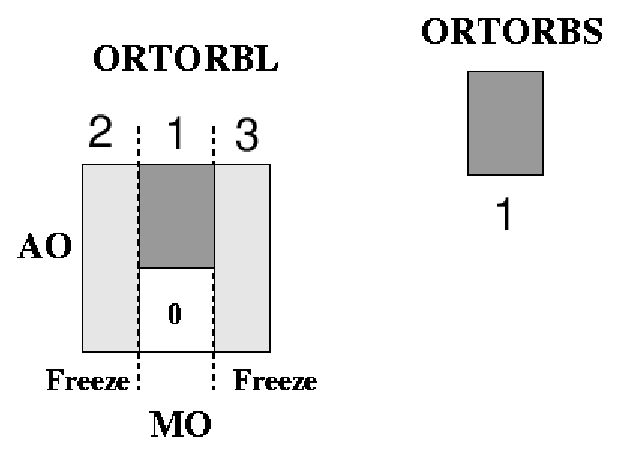
\includegraphics[width=7cm,keepaspectratio]{02_localization/images/matrix-2.eps}
\caption{\footnotesize A visual representation of the hierarchical
orthonormalization performed on the orbitals. The non-frozen orbitals
(marked with ``1'' in figure) are orthonormalized among themselves.
Then, frozen core orbitals (marked with ``2'' in figure) are orthonormalized
among themselves and against the non-frozen ones. Finally, the frozen
virtual orbitals (marked with ``3'') are orthonormalized against ``1'' and ``2''.
}
\label{fig:matrix-2}
\end{center}
\end{figure}



An additional effect must be considered responsible of the reported
behavior.  Further investigations, performed with the smaller system acetone
+ 2 H$_2$O, revealed a problem related to the molecular orbital hierarchical
orthonormalization (Fig.~\ref{fig:matrix-2}). After the cut action,
orbitals are no longer orthonormal, and the orthonormalization procedure
aims at restoring this orthonormality. 

The first class of orbitals performing the orthonormalization is the
non-frozen zone (marked ``1'' in Fig.~\ref{fig:matrix-2}) which remains
described in the smaller AO space. This class must be treated first, in
order to preserve itself inside this restricted space.

The second class is the frozen core orbitals class (marked ``2'' in
Fig.~\ref{fig:matrix-2}). When this class is orthonormalized with respect to
the first one, orthonormalization tails are produced, effectively changing
the core orbitals. The weight and spatial distribution of these tails is
bound to the atomic basis set used to describe the molecular system,
therefore larger basis sets produce stronger effects.

This situation is different from the previously reported phenomenon in
7Z-13 ammoniotridec-7-enoate in the frz-3/cut-3 analysis, where hydrogen
atoms were removed from non-frozen orbitals. In the current case, frozen
orbitals are modified due to orthonormality needs, which impose tails toward
nearby atoms. These tails introduce an artificial charge shift toward these
atoms, and in particular those involved in the physical process under
study, resulting in convergence problems or a high energy drift. The process
sometimes makes impossible for the evaluation to converge.

Molden plots have been performed on the smaller system with only two water
molecules. The contour factor is 0.03. Fig.~\ref{fig:acetone_tails} shows a
clear difference between the water OH bond with the Bas-C contraction and
the Bas-A contraction.

\begin{figure}[ht]
\begin{center}
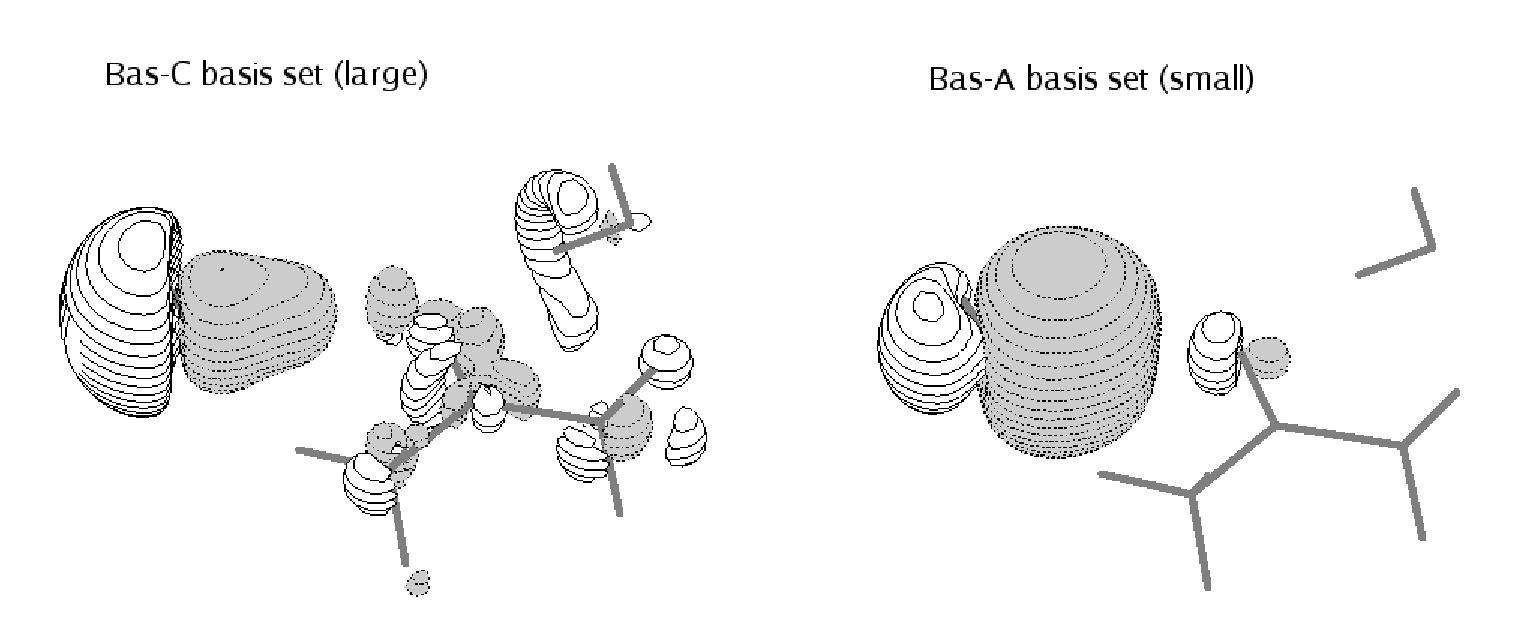
\includegraphics[width=12cm,keepaspectratio]{02_localization/images/acetone_tails.eps}
\caption{\footnotesize The water OH bond on the small acetone +
2H$_2$O system, using the large basis set Bas-C and the small Bas-A. The
difference in spatial distribution of the orthonormalization tails is
clearly visible. }
\label{fig:acetone_tails}
\end{center}
\end{figure}

\vspace{-5mm}
The nature of this problem is independent of the frozen spacer between the
removed zone and the non-frozen zone, but related to the frozen/non-frozen
seam. The problem do not arise when cut is not performed, and consequently
the resulting orbitals do not incur in orthonormalization. 

At first glance, a possible solution is to keep the frozen/non-frozen seam
as much far as possible from the region interested in the chemical
phenomenon, leading to absolute energy drifts but prevent tails to
act on the active space. However, this goes in the direction of incrementing
the computational cost of the final evaluation, enlarging the non-frozen
zone in a large basis regime.

Another possible solution has been attempted working with a non-orthonormal
basis set. Frozen orbitals are not orthonormalized with respect to the
non-frozen ones, and the results obtained (Tab.~\ref{tbl:acetone_basis}
non-ortho) show a cleaner behavior. However, it must be pointed out that this
procedure is not strictly formal under the assumptions made for the current
theoretical deployment, and the convergence is very slow. An improvement in
the theoretical asset is needed to formally work around this problem.

\section{Conclusions}

The Freeze-and-Cut technique has proved its usefulness in optimizing local
orbitals at CASSCF or quasi-CASSCF level. It combines the freeze of the
molecular orbitals that are not relevant for the phenomenon under study, and
the cut of those atoms that are not needed to describe the optimized
orbitals.

Different levels of theory can be used for the molecular framework and the
physically interesting region of the system.  The presented test cases
demonstrate the ability of the method to give essentially the same results
as a localized CASSCF calculation on the complete system, with a
significant reduction of the computational cost.

Two problems must be kept into account in order to obtain reliable CASSCF
energies: the first problem involves the tails of the unfrozen orbitals,
which can have a significant delocalization on the nearest neighbor atoms.
The projection of the unfrozen orbitals into a restricted set of atoms has
the effect of rising the absolute energy, but the relative energies seems to
be poorly affected. 

The second problem is relative to the methodological need to reorthonormalize
the frozen orbitals set after the cut is performed. This can introduce artificial
tails which can create instability when occurring near the active
orbitals. Both effects depend on the atomic basis set spatial distribution.

To face these problems, a general strategy can be devised:
\begin{itemize}
\item reduce the cut out of the unfrozen orbitals, setting the cut seam
far from the unfrozen region. Atoms which are geometrically very distant
from the unfrozen set can be usually cut out safely
\item reduce the influence of the frozen orbitals orthonormalization tails 
on the chemically active region (usually, the active orbitals).  To minimize
this effect, a sufficient spacer of unfrozen orbitals should be kept.
\end{itemize}
Further evaluations are however needed to gain detailed comprehension of
this strategy.


\clearpage
\pagestyle{empty}{\ }\\
\clearpage
\pagestyle{empty}
\begin{center}
{\Huge \textbf Resum\'e chapitre \ref{chp:nevpt} \\ NEVPT }
\end{center}

Les th\'eories perturbatives multir\'ef\'erence sont des instruments importants
pour l'\'evaluation de l'\'energie de corr\'elation sur mol\'ecules petites et
moyennes. L'avantage de l'approche perturbative est la r\'eduction du co\^ut
computationnel: \`a parit\'e de qualit\'e des r\'esultats, une approche
variationnelle est plus lourde. Seulement en temps r\'ecents les approches
perturbatives multireference sont utilis\'ees intensivement dans la recherche
en chimie quantique.

L'objectif des th\'eories perturbatives multir\'ef\'erence est la cr\'eation
d'une approche vite et propre, correspondante \`a l'approche \`a single
d\'eterminant M{\o}ller-Plesset (MP). Quand on travaille sur des syst\`emes
bien d\'ecrits avec un seul d\'eterminant, la th\'eorie M{\o}ller-Plesset au
deuxi\`eme ordre donne plus de 90 \% de l'\'energie de corr\'elation.

Quand le syst\`eme \'etudi\'e n\'ecessite d'une approche multir\'ef\'erence, et donc la
fonction d'onde d'ordre z\'ero est multir\'ef\'erence, le d\'eveloppement d'une
th\'eorie perturbative est plus complexe. Le probl\`eme est la d\'efinition
d'un Hamiltonien d'ordre z\'ero appropri\'e. Si ce choix n'est pas bon, on
obtient une th\'eorie perturbative que
\begin{itemize}
\item \textbf{n'est pas size consistent}: l'\'energie de deux syst\`emes
qui n'interagissent pas entre eux, AB, doit \^etre \'egale al'\'energie
qui on obtient en faisant le calcul sur chacune et en faisant l'addition
(E$_{AB} = $E$_A + $E$_B$)
\item \textbf{\`a des \'etats intrus}, quand les fonctions perturbatives
ont des \'energies presque \'egales \`a l'\'energie de la fonction d'ordre z\'ero.
Ce probl\`eme donne lieu \`a un comportement divergent.
\end{itemize}

La th\'eorie n-Electron Valence state Perturbation Theory est une
th\'eorie perturbative multir\'ef\'erence qui travaille sur une fonction d'onde de
type Complete Active Space (CAS). Elle a \'et\'e d\'evelopp\'ee \`a Ferrara en collaboration avec l'universit\'e
Paul Sabatier de Toulouse.  La m\'ethode adresse \`a la fois le probl\`eme
de size consistency et le probl\`eme des \'etats intrus, et donne l'approche
M{\o}ller-Plesset si on effectue le calcul sur une fonction d'onde \`a un
seul d\'eterminant.

Le d\'eveloppement theoretique utilise un Hamiltonien bielectronique,
l'Hamiltonien de Dyall, qui donne une th\'eorie propre et efficiente. Les
fonctions perturbatives sont de nature multir\'ef\'erencielle, et peuvent
\^etre classifi\'ee dans huit classes d'excitation, selon le sch\'ema de
promotion des electrons. 

La th\'eorie a deux niveaux de pr\'ecision, ``Strongly Contracted'' et ``Partially
Contracted'', selon la contraction de l'espace perturbatif.
La Strongly Contracted NEVPT utilise un espace monodimensionnel pour chaque
classe, et la Partially Contracted utilise un espace \`a dimensionalit\'e
plus haute, mais plus petite que l'espace complet des determinants
excit\'es.  L'approche Strongly Contracted donne des r\'esultats de bonne
qualit\'e si compar\'ee avec la Partially Contracted. Une diff\'erence entre
eux est normalement un sympt\^ome d'une mauvaise d\'escription \`a
l'ordre-zero.

Dans cette th\`ese, diff\`erent types de NEVPT ont \'et\'e d\'evelopp\'e
et utilis\'e:
\begin{itemize}
\item Single State NEVPT, qui fait la correction perturbative \`a un seul
\'etat \'electronique
\item Quasi Degenerate NEVPT, qui fait cette correction \`a un
ensemble d'\'etats \'electroniques simultan\'ement.  Cette approche
consid\`ere les interactions entre les fonctions d'onde apr\`es la
perturbation, et permit le m\'elange de ce fonctions.
\item Non Canonical NEVPT, est une extension de l'approche single \'etat qui
travaille avec des orbitales qui ne sont pas canoniques (elles ne diagonalisent
pas la matrice de Fock g\'en\'eralis\'ee). Cette approche est tr\`es utile
pour l'integration entre Localisation et NEVPT, parce que les resultats sont
invariables pour le m\'elange des orbitales de core et virtuelles, et donc
il permit l'utilisation directe avec un ensemble d'orbitales localis\'ees.
\end{itemize}

L'approche Single-State a \'et\'e utilis\'ee pour effectuer des calculs sur les
mol\'ecules de formaldehyde, acetaldehyde et ac\'etone. Tous ces mol\'ecules ont
un groupe carbonyle, et diff\'erents strat\'egies ont \'et\'e appliqu\'ees pour avoir
une compr\'ehension directe des \'etats excit\'es de ce groupe fondamental. En
particulier, on a effectu\'e l'\'evaluation de l'\'energi\'e des \'etats
excit\'es de valence, soit adiabatiques que verticales, et des \'etats
Rydberg. Pour les \'etats adiabatiques, on a aussi \'evalu\'e l'\'energie
de point z\'ero (ZPE) vibrationnel, les g\'eom\'etries et le comportement
vibrationnel des \'etats excit\'es de valence.

Avec l'approche Quasi-Degenerate on a \'etudi\'e la courbe de potentiel du
ground state, deux \'etats rydberg et du $\pi \rightarrow \pi^{*}$ contre le
stretching C-O, dans la mol\'ecule de formaldehyde. Le courbes obtenues \`a niveau
CASSCF ont des croisements \'evit\'es, et l'application de la NEVPT
Quasi-Degenerate donne des courbes plut\^ot diff\`erentes sur la position e la
forme des ces croisements.  Les r\'esultats de la th\'eorie QD-NEVPT peuvent
\^etre amelior\'ees avec une procedure iterative, qui peut \^etre une bonne
solution \`a des probl\'emes dans les r\'esultats obtenus.

Enfin, une \'evaluation pr\'eliminaire a \'et\'e effectu\'e avec la NEVPT
Non-Canonique sur un syst\`eme localis\'e. Les valeurs obtenues d\'emontrent la validit\'e
de cette approche, qui sera fondamentale pour l'int\'egration directe de la
th\'eorie de localisation des orbitals mol\'eculaires et la th\'eorie NEVPT.


\cleardoublepage
\pagestyle{fancy}
\chapter{NEVPT}
\label{chp:nevpt}
%\pagenumbering{arabic}

Multireference perturbation theories are important tools for the
evaluation of the correlation energy in small and medium sized molecules.
The main advantage of a perturbative approach is the reduced computational
cost when compared to a completely variational treatment, still providing a
good level of accuracy.  First attempts in deploying theoretical approaches
for MRPT are quite old\cite{rmp-39-771-1967,jcp-58-5745-1973} but these
approaches began to be mainstream only recently.

The goal of multireference perturbation theories is the creation of a quick
and accurate tool resembling the single-determinant based M{\o}ller-Plesset
(MP) approach\cite{pr-46-618-1934}, extended to a multireference context:
when the molecular system under study is well described by a
single-reference treatment, second-order M{\o}ller-Plesset perturbation
theory gives more than 90\% of the correlation energy. The zero-order
Hamiltonian is defined as the $n$ particles Fock operator 
\beq
\ham_0 = \sumonen{i} \fock(i)
\eeq
which leads to the wavefunction correction
\beq
\Psi_n^{(1)} = - \sum_{k \neq n} \ket{\Psi_k^{(0)}}
\frac{\braket{\Psi_k^{(0)}}{\perturb}{\Psi_n^{(0)}}}{E_k^{(0)} -
E_n^{(0)}}
\eeq
and to the well known second-order M{\o}ller-Plesset correction for the energy
\beq
E_0^{(2)} = - \sum_{i,j}^{\mbox{\tiny occ}} \sum_{r,s}^{\mbox{\tiny virt}} \frac{\left|
\interact{rs}{ij}\right|^{2}}{\epsilon_r + \epsilon_s - \epsilon_i -
\epsilon_j }
\eeq
where $\epsilon$ are the orbital energies associated to each orbital

Unfortunately, with a multireference zero-order wavefunction the application
of a perturbative approach is more difficult, due to the complex definition
of a zero-order Hamiltonian.  When a choice has been made, various kind of
problems arise, preventing the deployment of an easy-to-use perturbative
scheme for multireference wavefunctions. 

These problems can be accounted as the following:
\begin{itemize}
\item \textbf{lack of size consistency} (strict separability), which
requires the energy of two non-interacting systems AB to be equal to the sum
of the energies of A and B treated independently (E$_{AB} = $E$_A + $E$_B$)
\item ``\textbf{intruder states}'', when the perturbers happen to have very similar
energies to the zero-order wavefunction, leading to divergent behavior due
to the nearly zero denominator in the perturbation theory equations.
The M{\o}ller-Plesset treatment is not affected by this problem, since the
perturbers are the doubly excited determinants $\Phi_{ij}^{rs}$, and the
corresponding energies are $E_0 + \epsilon_r + \epsilon_s - \epsilon_i -
\epsilon_j$, well distinct from $E_0$.
\item \textbf{different levels of accuracy for ground and excited states}, making the
evaluation of transition energy more complex.
\item \textbf{no spin purity}, leading for example to a mix between singlet and triplet
wavefunctions. This introduces additional complexity for spectroscopical
evaluations, and spin-based property evaluations.
\item \textbf{efficiency}. The perturbative treatment is required to be fast and with
reduced disk space and memory footprints.
\end{itemize}

\subsection*{Classification of perturbative methods}

Multireference perturbation theories can be classified in two categories:
``\textit{perturb then diagonalize}'', where an effective Hamiltonian is built
and then diagonalized \cite{rmp-39-771-1967,jpa-18-809-1985}, and
``\textit{diagonalize then perturb}'', where the perturbative treatment is
applied to a variationally optimized wavefunction. 

To the latter category belong for example CIPSI techniques, started by
Huron \textit{et al.}\cite{jcp-58-5745-1973} in Paris and subsequently
developed in Pisa\cite{jcc-8-39-1987} and Ferrara
\cite{ijqc-60-167-1996,tca-98-57-1997,tca-98-117-1997,tca-105-259-2001}.
CIPSI uses single determinants as perturbers, using a baricentric
M{\o}ller-Plesset or a diagonal bielectronic
(Epstein-Nesbet\cite{pr-28-695-1926,prsl-230-312-1955}) zero-order
Hamiltonian. Although numerically efficient
\cite{ijqc-60-167-1996,tca-98-57-1997,tca-98-117-1997,jcp-83-1746-1985}, it lacks some formal
requirement, like strict separability. Other analogous methods
\cite{jcp-90-3647-1997,cpl-190-374-1992,jcp-94-5021-1991,cpl-183-443-1991, cpl-222-615-1994}
suffer from similar problems.

Another ``\textit{diagonalize then perturb}'' method is the CASPT2
approach\cite{jpc-94-5483-1990,jcp-96-1218-1992}. It makes use of contracted
perturbers obtained from a CASCI under the action of excitation operators,
and a one-electron zero-order Hamiltonian. Due to its efficiency, CASPT2 is
applicabile to large CAS spaces, providing good results for ground and
excited states at a reasonable computational cost. Integration into
the \textit{ab initio} suite \molcas makes CASPT2 one of the most used post
Hartree-Fock treatments.  The main problem of the method is its sensibility
to intruder states, leading to incorrect or divergent behavior. 

$n$-Electron Valence Perturbation Theory (NEVPT) approach
\cite{jcp-114-10252-2001,jcp-117-9138-2002,cpl-350-297-2001} is a
``\textit{diagonalize then perturb}'' method developed and implemented in
Ferrara and Toulouse. The method formally addresses both strict separability
and intruder states problems, and also comes as a natural extension to
M{\o}ller-Plesset. In fact, second-order NEVPT (NEVPT2) formally reproduces
the M{\o}ller-Plesset equations when applied to a single-reference
wavefunction.

In the development of NEVPT two levels of approximations have been
considered:
\begin{itemize}
\item the degree of contraction of the perturber space, and therefore, of
the perturber wavefunctions
\item the choice of the zero-order Hamiltonian
\end{itemize}

%nevpt single state
\section{Single-State NEVPT}

Let $\Psi_m^{(0)}$ be a zero-order CASCI wavefunction
\beq
\Psi_m^{(0)} = \sumidx{I \in \mbox{\tiny CAS}} C_{I,m} \ket{I}
\eeq
obtained diagonalizing $\ham$ inside the CAS
\beq
\proj{\mbox{\tiny CAS}}\ham\proj{\mbox{\tiny CAS}}\ket{\Psi_m^{(0)}} = E_m^{(0)} \ket{\Psi_m^{(0)}}
\eeq
where $\proj{\mbox{\tiny CAS}}$ is the projector inside the CASCI space. 

We can define perturbers in NEVPT as zero-order wavefunctions of the outer
space (external to CAS) where $k$ electrons are removed from the inactive
part and added to the valence part. If we decompose the zero-order CASCI
wavefunction as an antisymmetrized product of an inactive part (made of both
core and virtual orbitals) with $n_c$ electrons, and a valence part (made of
active orbitals) with $n_v$ electrons
\beq
\ket{\Psi_m^{(0)}} = \ket{\Phi_c \Psi_m^v}
\eeq
then the perturber wavefunctions can be expressed as
\beq
\ket{\Psi_{l,\mu}^{k}} = \ket{\Phi_l^{-k} \Psi_{\mu}^{v+k}}
\eeq
where $l$ is a collective index that describes the orbitals involved in the
operation and $\mu$ an enumerator index for the different wavefunctions. At
second order of perturbation $-2 \le k \le 2$.  

A graphical representation of the excitation scheme for NEVPT can be seen in
Fig. \ref{fig:classes}

\begin{center}
\begin{figure}[ht]
\begin{center}
\includegraphics[width=9cm,angle=270]{03_nevpt/images/classes.ps}
\end{center}
\caption{\footnotesize The eight excitation classes defining the perturber
functions in NEVPT.}
\label{fig:classes}
\end{figure}
\end{center}


The perturbers functions span a space of determinants with the same inactive
part $\Phi_l^{-k}$ and all the possible valence parts $\Psi_I^{+k}$. These
spaces are denoted as $S_l^k$
\beq
S_{l}^{k} \equiv \left\{ \Phi_l^{-k} \Psi_I^{+k} \right\}
\eeq
Perturbers will be defined in these spaces. If the full dimensionality
is exploited, the resulting approach is called \textit{totally
uncontracted}. The perturbers and their energies can be obtained by
diagonalizing the Hamiltonian inside each space
\beq
\label{eqn:teoria1_1}
\proj{S_l^k}\ham\proj{S_l^k} \ket{\Phi_l^{-k} \Psi_{\mu}^{v+k}} = E_{l,\mu}
\ket{\Phi_l^{-k} \Psi_{\mu}^{v+k}}
\eeq
however, this procedure is impractical given its high computational cost.
For each $S_l^k$ space, a diagonalization of the true Hamiltonian must be performed.

We can improve the computational asset by introducing a modified
Hamiltonian, proposed by Dyall\cite{jcp-102-4909-1995}
\beqa
\ham^D &=& \ham^D_i + \ham^D_v + C \\
\ham^D_i &=& \sum_{i}^{\mbox{\tiny core}} \epsilon_i E_{ii} +
\sum_r^{\mbox{\tiny virt}} \epsilon_r E_{rr} \\
\ham^D_v &=& \sum_{ab}^{\mbox{\tiny act}} h_{ab}^{\mbox{\tiny eff}} E_{ab} +
\frac{1}{2} \sum_{abcd}^{\mbox{\tiny act}} \integral{ab}{cd} \left( E_{ac}
E_{bd} - \delta_{bc} E_{ad} \right) \\
C &=& 2 \sum_{i}^{\mbox{\tiny core}} h_{ii} + \sum_{ij}^{\mbox{\tiny core}}
\left( 2 \integral{ij}{ij} - \integral{ij}{ji} \right) - 2
\sum_{i}^{\mbox{\tiny core}} \epsilon_i
\eeqa
where labels $i,j,\ldots$, $a,b,\ldots$, $r,s,\ldots$ denote core, active
and virtual orbitals respectively, and this convention will be retained
hereafter, $\epsilon_i$ and $\epsilon_r$ are the orbital energies of the
involved orbitals, and $E_{mn}$ operators are the spin-traced operators
$\constr{m\alpha}\destr{n\alpha} + \constr{m\beta}\destr{n\beta}$. These
operators commute with $S^2$ and $S_z$, therefore the application of these
operators on a spin-pure function produces again a spin-pure function.
Finally, the $h_{ab}^{\mbox{\tiny eff}}$ matrix evaluates as
\beq
h_{ab}^{\mbox{\tiny eff}} =  h_{ab} + \sum_j \left( 2 \integral{aj}{bj} -
\integral{aj}{jb} \right)
\eeq

$\ham^D$ behaves like the true Hamiltonian inside the CAS space, having the
same eigenvalues and eigenvectors of the true Hamiltonian projected onto the
CAS space. Also, given the decomposition for the wavefunction defined
before, the action of the Dyall's Hamiltonian can be partitioned
\beq
\ham^D \ket{\Phi_l^{-k} \Psi_{\mu}^{v+k}} = E_{l,\mu}^{k} \ket{\Phi_l^{-k}
\Psi_{\mu}^{v+k}} 
\eeq
stripping out the constant contribution of the inactive part and leaving a
subsystem to be solved for the valence part
\beq
\ham^D_v \ket{\Psi_{\mu}^{v+k}} = E_{\mu}^{k} \ket{\Psi_{\mu}^{v+k}} 
\eeq
The total energy $E_{l,\mu}^{k}$ is the sum of $E_{\mu}^{k}$ and the 
energies of the orbitals involved in the definition of the inactive part
$\Phi_l^{-k}$. This introduces the possibility to perform a single
diagonalization of the valence Dyall's Hamiltonian on the CASCI zero-order
wavefunction and evaluate the perturber energies using the property depicted
above.

\subsection*{Strongly Contracted approach}

A possible choice in the development of the NEVPT approach is to choose a
single function for each space $S_l^k$, leading to the \textit{Strongly
Contracted (SC)} scheme. A set of perturbative operators are used to produce a
single function for each space, according to the following definition
\beq
\Psi_l^k = \proj{S_l^k} \ham \Psi_m^{(0)}
\eeq
where $\proj{S_l^k}$ is the projector onto the subspace $S_l^k$. The same
result can be obtained by applying a specific part of the Hamiltonian to the
zero-order wavefunction
\beq
\Psi_l^k = V_l^k \Psi_m^{(0)}
\eeq

For each space, an appropriate operator can be devised
\beqa
V_{ijrs}^{0} &=& \gamma_{ij} \gamma_{rs} \left( \integral{rs}{ij} E_{ri} E_{sj} + \integral{rs}{ji} E_{si} E_{rj} \right) \quad i \le j, r \le s \\
V_{rsi}^{-1} &=& \gamma_{rs} \sum_a \left( \integral{rs}{ia} E_{ri} E_{sa} + \integral{sr}{ia} E_{si} E_{ra} \right) \quad  r \le s \\
V_{ijr}^{1} &=& \gamma_{ij} \sum_a \left( \integral{ra}{ji} E_{rj} E_{ai} + \integral{ra}{ij} E_{ri} E_{aj} \right) \quad  i \le j \\
V_{rs}^{-2} &=& \gamma_{rs} \sum_{ab} \integral{rs}{ba} E_{rb} E_{sa} \quad  r \le s \\
V_{ij}^{2} &=& \gamma_{ij} \sum_{ab} \integral{ba}{ij} E_{bi} E_{aj} \quad  i \le j \\
V_{ir}^{0} &=& \sum_{ab} \left( \integral{ra}{ib} E_{ri} E_{ab} + \integral{ra}{bi} E_{ai} E_{rb} \right) + h_{ri}^{\mbox{\tiny eff}} E_{ri} \\
V_r^{-1} &=& \sum_{abc} \integral{ra}{bc} E_{rb} E_{ac} + \sum_{a} h_{ra}^{\mbox{\tiny eff'}} E_{ra} \\
V_i^{1} &=& \sum_{abc} \integral{ba}{ic} E_{bi} E_{ac} + \sum_{a} h_{ai}^{\mbox{\tiny eff}} E_{ai}
\eeqa
where $\gamma_{mn} = 1 - \half \delta_{mn}$.

Auxiliary matrixes have been also defined as
\beqa
h_{mn}^{\mbox{\tiny eff}} &=& h_{mn} + \sum_j \left( 2 \integral{mj}{nj} -
\integral{mj}{jn} \right) \\
h_{mn}^{\mbox{\tiny eff'}} &=& h_{mn}^{\mbox{\tiny eff}} - \sum_b
\integral{mb}{bn}
\eeqa
The perturber functions are not normalized. The norm of these functions
\beq
N_l^k = \integral{\Psi_l^k}{\Psi_l^k} = \braket{\Psi_m^{(0)}}{
\left(V_l^k\right)^+  V_l^k }{\Psi_m^{(0)}}
\eeq
plays an important role in the Strongly Contracted development. The values
of the norms for each function are
\beqa
N_{ijrs}^{0} &=& 4 \gamma_{ij} \gamma_{rs} \left( \integral{rs}{ij}^2 + \integral{rs}{ji}^2 - \integral{rs}{ij}\integral{rs}{ji} \right) \\
%
N_{rsi}^{-1} &=& \gamma_{rs} \sum_{ab} \left[ 2 \left(\integral{rs}{ib}\integral{rs}{ia} + \integral{sr}{ib}\integral{sr}{ia} \right) \right. \nonumber \\
& & \left. - \integral{rs}{ib} \integral{sr}{ia} - \integral{sr}{ib} \integral{rs}{ia}\right] R_{ba}^{(1)} \\
%
N_{ijr}^{1} &=& \gamma_{ij} \sum_{ab} \left[ 2 \left(\integral{rb}{ji}\integral{ra}{ji} + \integral{rb}{ij}\integral{ra}{ij} \right) \right. \nonumber \\
& & \left. - \integral{rb}{ji} \integral{ra}{ij} - \integral{rb}{ij}
\integral{ra}{ji}\right] \tilde{R}_{ba}^{(1)} \\
N_{rs}^{-2} &=& \gamma_{rs} \sum_{abcd} \integral{rs}{ba} \integral{rs}{dc} R_{abcd}^{(2)} \\
%
N_{ij}^{2} &=& \gamma_{ij} \sum_{abcd} \integral{ba}{ij} \integral{dc}{ij} \tilde{R}_{abcd}^{(2)} 
\eeqa
\beqa
N_{ir}^{0} &=& \sum_{abcd} \left[ \left( 2
\integral{ra}{ib}\integral{rc}{id} - \integral{ra}{ib}\integral{rc}{di} - \integral{ra}{bi} \integral{rc}{id} \right) \braket{\Psi_m^{(0)}}{E_{ba}E_{cd}}{\Psi_m^{(0)}} \right. \nonumber \\
& & \left. + \integral{ra}{bi} \integral{rc}{di} \left( \braket{\Psi_m^{(0)}}{E_{bd}\tilde{E}_{ac}}{\Psi_m^{(0)}} + \delta_{ab} R_{ba}^{(1)}\right) \right] \nonumber\\
& & + 2 \sum_{ab} \left(2 \integral{ra}{ib} - \integral{ra}{bi} \right) h_{ri}^{\mbox{\tiny eff}} R_{ba}^{(1)} + 2 \left( h_{ri}^{\mbox{\tiny eff}}\right)^2 \\
%
N_{r}^{-1} &=& \sum_{abcdef} \integral{rd}{ef} \integral{ra}{bc} \braket{\Psi_m^{(0)}}{E_{fd}E_{eb}E_{ac}}{\Psi_m^{(0)}} \nonumber \\
&& + 2 \sum_{abcd} \integral{ra}{bc} h_{ra}^{\mbox{\tiny eff'}} \braket{\Psi_m^{(0)}}{E_{ca}E_{bd}}{\Psi_m^{(0)}} \nonumber \\
&&+ \sum_{ab} h_{ra}^{\mbox{\tiny eff'}} h_{rb}^{\mbox{\tiny eff'}} R_{ba}^{(1)} \\
%
N_{i}^{1} &=& \sum_{abcdef} \integral{ed}{if} \integral{ba}{ic} \braket{\Psi_m^{(0)}}{E_{fd}\tilde{E}_{eb}E_{ac}}{\Psi_m^{(0)}} \nonumber \\
&&+ 2 \sum_{abcd} \integral{ba}{ic} h_{di}^{\mbox{\tiny eff}} \braket{\Psi_m^{(0)}}{E_{ca}\tilde{E}_{bd}}{\Psi_m^{(0)}} \nonumber\\
&&+ \sum_{ab} h_{ai}^{\mbox{\tiny eff}} h_{bi}^{\mbox{\tiny eff}} \tilde{R}_{ba}^{(1)}
\eeqa
To evaluate these norms, the spinless density matrix of rank not higher than
three between the $\Psi_m^{(0)}$ functions are needed.  A short notation has
been used for the hole density matrixes
\beqa
\tilde{R}_{ab}^{(1)} &=& 2 \delta_{ab} - R_{ba}^{(1)} \\
\tilde{R}_{abcd}^{(2)} &=& R_{abcd}^{(2)} + \delta_{ad} R_{cb}^{(1)} + \delta_{bc} R_{da}^{(1)} - 2 \delta_{ac} R_{db}^{(1)} \\
& & - 2 \delta_{bd} R_{ca}^{(1)} - 2 \delta_{ad} \delta_{bc} + 4 \delta_{ca} \delta_{db}
\eeqa
and for the operator $\tilde{E}_{ab} = 2 \delta_{ab} - E_{ba}$

An important property of the $\Psi_{l}^{k}$ is that any other function of
the space $S_l^k$ which is orthogonal to  $\Psi_{l}^{k}$ do not interact
with the zero-order wavefunction through the true Hamiltonian. It is
possible to use the  $\Psi_{l}^{k}$ functions as a basis set for the
expansion of the first-order correction to the wavefunction, and also for
the expression of the zero-order Hamiltonian by means of a spectral
decomposition
\beq
\ham_0 = \sum_{lk} \ket{ {\Psi_{l}^{k}}' } E_{l}^{k} \bra{ {\Psi_{l}^{k}}' } +
\sum_{m}  \ket{\Psi_{m}^{(0)}} E_{m}^{(0)} \bra{\Psi_{m}^{(0)}}
\eeq
where $\ket{ {\Psi_{l}^{k}}' }$ are the normalized $\ket{ \Psi_{l}^{k} }$. 

The expression for the first-order correction to the wavefunction is
therefore
\beqa
\Psi_m^{(1)} &=& \sum_{kl} \ket{{\Psi_{l}^{k}}'}
\frac{\braket{{\Psi_{l}^{k}}'}{\ham}{\Psi_{m}^{(0)}}}{E_m^{(0)} - E_{l}^{k}} \\
&=& \sum_{kl} \ket{{\Psi_{l}^{k}}'} \frac{\sqrt{N_l^k}}{E_{m}^{(0)} - E_{l}^{k}} 
\eeqa
and for the energy is
\beq
E_{m}^{(2)} = \sum_{kl} \frac{\braket{{\Psi_{l}^{k}}'}{\ham}{\Psi_{m}^{(0)}}^2} {E_m^{(0)} - E_{l}^{k}} = \sum_{kl} \frac{N_l^k}{E_m^{(0)} - E_{l}^{k}}
\eeq
however, we still miss a definition of the perturber energies $E_l^k$.
These energies can be defined in a computationally advantageous approach, by
means of the Dyall's Hamiltonian.
\beq
E_{l}^{k} = \frac{1}{N_l^k} \braket{\Psi_{l}^{k}}{\ham^D}{\Psi_{l}^{k}}
\eeq
which leads to
\beqa
N_{l}^{k} E_{l}^{k} &=& \braket{\Psi_{m}^{(0)}}{{V_{l}^{k}}^{+} \ham^D
V_{l}^{k}}{\Psi_{m}^{(0)}} \\
 &=& \braket{\Psi_{m}^{(0)}}{{V_{l}^{k}}^{+} V_{l}^{k}
\ham^D}{\Psi_{m}^{(0)}} + \braket{\Psi_{m}^{(0)}}{{V_{l}^{k}}^{+}
\commut{\ham^D}{V_{l}^{k}} }{\Psi_{m}^{(0)}} 
\eeqa
Developing the braket and extracting the inactive part of the Dyall's
Hamiltonian we obtain
\beq
E_{l}^{k} = E_m^{(0)} + \Delta \epsilon_l + \frac{1}{N_l^k}
\braket{\Psi_{m}^{(0)}}{{V_{l}^{k}}^{+}
\commut{\ham_v}{V_{l}^{k}} }{\Psi_{m}^{(0)}}
\eeq
with $\Delta \epsilon_l$ is the sum of the orbital energies of the newly
occupied virtual orbitals minus the orbital energies of the unoccupied core
orbitals. 

The term that still need to be evaluated is the braket involving the
commutator. After development of each $V$ operator and substitution, we
obtain the contributions to the energy. Here we present the result for
$V_{rsi}^{(-1)}$:
\beqa
\braket{\Psi_{m}^{(0)}}{V_{rsi}^{(-1)}
\commut{\ham_v}{V_{rsi}^{(-1)}}}{\Psi_{m}^{(0)}} &=& \gamma_{rs} \sum_{ab}
\left[ 2 \left( \integral{rs}{ia} \integral{rs}{ib} + \integral{sr}{ia}
\integral{sr}{ib} \right) \right. \nonumber \\
&&\left. -\left( \integral{rs}{ia} \integral{sr}{ib} + \integral{sr}{ia}
\integral{rs}{ib}\right) \right] K_{ab} \nonumber \\
\eeqa
where $K_{ab}$ is analogous to a spin-free formulation of the Koopmans
matrix, defined only in the active space
\beqa
\label{eqn:koopmans_matrix}
K_{ab} &=& \half \braket{\Psi_{m}^{(0)}}{E_{as}E_{ir} \commut{\ham_v}{E_{ri}E_{sb}}}{\Psi_{m}^{(0)}} \\
&=& \sum_{c} h_{ac}^{\mbox{\tiny eff}} R_{bc}^{(1)} - \sum_{cde} \integral{cb}{ed} R_{acde}^{(2)} 
\eeqa
The contribution of the $\Psi_{rsi}^{-1}$ is therefore given by
\beq
E_m^{(2)}\left( S_{rsi}^{-1} \right) = - \frac{N_{rsi}^{-1}}{\epsilon_r
+\epsilon_s - \epsilon_i - \epsilon_{rsi}^{-1}}
\eeq
with
\beq
\epsilon_{rsi}^{-1} = \frac{1}{N_l^k}
\braket{\Psi_{m}^{(0)}}{{V_{rsi}^{-1}}^{+}
\commut{\ham_v}{V_{rsi}^{-1}} }{\Psi_{m}^{(0)}}
\eeq

An interesting case is the $V_{ijrs}^{(0)}$ case, which is identical to the
M{\o}ller-Plesset contribution 

\beq
E_m^{(2)}\left( S_{rsij}^{0} \right) = - \frac{N_{rsij}^{0}}{\epsilon_r
+\epsilon_s - \epsilon_i - \epsilon_{j}}
\eeq

NEVPT2 can therefore be seen as a generalized form of MP2 to multireference
wavefunctions, and this result is also found in the completely uncontracted
and Partially Contracted approaches\cite{cpl-317-472-2000}.

The cases involving the $V_{rs}^{-2}$  and $V_{ij}^{2}$ operators require
the knowledge of the three-particles density matrix, and the $V_{r}^{-1}$
and $V_{i}^{1}$ require auxiliary matrixes depending on the four-particles
density matrixes. All these matrixes always involve only the active indexes,
therefore represent only a minor issue for nowadays computers.

\subsection*{Partially Contracted approach}

An alternative approach, named \textit{Partially Contracted
(PC)}, is to use a subspace $\overline{S}_l^k$ of $S_l^k$.
To define this subspace, a set of functions $\Phi$ is generated by means of
the $V_l^k$ operators. These functions must be orthonormalized and purged of
linear dependencies which may arise. The resulting set spans the
$\overline{S}_l^k$ space.

Once the $\overline{S}_l^k$ spaces have been defined, we can obtain a set of
perturbers
\beq
\proj{\overline{S}_l^k}\ham\proj{\overline{S}_l^k} \ket{\Psi_{l\mu}^{k}} =
E_{l,\mu}^{k} \ket{\Psi_{l\mu}^{k}}
\eeq
where we can substitute $\ham$ with $\ham^D$ to simplify the evaluation.
Perturbers are generated by the application of the excitation operators
without contraction. For example, in the case of the $V_{rsi}^{-1}$ operator
\beq
V_{rsi}^{-1} = \gamma_{rs} \sum_a \left( \integral{rs}{ia} E_{ri} E_{sa} + \integral{sr}{ia} E_{si} E_{ra} \right) \quad  r \le s
\eeq
the Partially Contracted approach makes use of functions $\Phi_{risa} =
E_{ri} E_{sa} \Psi_m^{(0)}$ and $\Phi_{risa} = E_{si} E_{ra} \Psi_m^{(0)}$.
We can group these functions in two row vectors $\mathbf{\Phi}_{ris}$ and
$\mathbf{\Phi}_{sir}$ to write the expression of the overlap and $\ham^D$
matrixes
\beq
\integral{\mathbf{\Phi}_{ris}, \mathbf{\Phi}_{sir} }{\mathbf{\Phi}_{ris},
\mathbf{\Phi}_{sir}} = 
\left[ 
\begin{array}{cc}
2 R^{(1)} & - R^{(1)} \\
- R^{(1)} & 2 R^{(1)} 
\end{array}
\right]
\eeq
\beqa
\braket{\mathbf{\Phi}_{ris}, \mathbf{\Phi}_{sir} }{\ham^{D}}{\mathbf{\Phi}_{ris},
\mathbf{\Phi}_{sir}} & = & \left[ 
\begin{array}{cc}
2 \mathbf{K} & - \mathbf{K} \\
- \mathbf{K} & 2 \mathbf{K}
\end{array}
\right] \nonumber \\
&  & + \left( E_m^{(0)} +\epsilon_r +\epsilon_s - \epsilon_i \right)
\left[ 
\begin{array}{cc}
2 \mathbf{R}^{(1)} & - \mathbf{R}^{(1)} \\
- \mathbf{R}^{(1)} & 2 \mathbf{R}^{(1)} 
\end{array}
\right] \nonumber \\
\eeqa
where $\mathbf{R}^{(1)}$ is the one-particle density matrix in the spinless
formulation and the $\mathbf{K}$ matrix is defined as \ref{eqn:koopmans_matrix}
The diagonalization of the $\ham^D$ matrix is quickly obtained diagonalizing
$\mathbf{K}$ in the metric $\mathbf{R}^{(1)}$ to obtain $\mathbf{c}_{\mu}$ coefficients and
$\epsilon_{\mu}$ energies
\beq
\mathbf{K} \mathbf{c}_{\mu} = - \epsilon_{\mu} \mathbf{R}^{(1)} \mathbf{c}_{\mu}
\eeq
to obtain two distinct orthonormal functions
\beqa
\Psi_{ris\mu}^{-1} = \frac{1}{\sqrt{2}} \sum_{a} c_{a \mu} \left( \Phi_{risa} +
\Phi_{sira} \right) \\
{\Psi_{ris\mu}^{-1}}' = \frac{1}{\sqrt{6}} \sum_{a} c_{a \mu} \left( \Phi_{risa} -
\Phi_{sira} \right)
\eeqa
These functions will be used in the evaluation of the interaction with the
zero-order wavefunction. We define
\beqa
\left( rs, \mu i \right) &=& \braket{\Psi_{ris\mu}^{-1}}{\ham}{\Psi_{m}^{(0)}} \\
                         &=& \frac{1}{\sqrt{2}} \sum_{a} \left( \integral{rs}{ia} + \integral{sr}{ia} \right) S_{a \mu}
\eeqa
\beqa
{\left( rs, \mu i \right)}' &=& \braket{{\Psi_{ris\mu}^{-1}}'}{\ham}{\Psi_{m}^{(0)}} \\
                         &=& \sqrt{\frac{3}{2}} \sum_{a} \left( \integral{rs}{ia} - \integral{sr}{ia} \right) S_{a \mu}
\eeqa
where 
\beq
S_{a \mu} = \sum_{a'}  c_{a \mu}^{*} R_{a' a}^{(1)}
\eeq
We can now finally write the contribution for this subspace to the
second-order energy
\beq
E^{(2)}(\overline{S}_{rsi}^{-1}) = - \sum_{\mu} \frac{\left( rs, \mu
i\right)^2 + {\left( rs, \mu 
i\right)'}^2}{\epsilon_r + \epsilon_s - \epsilon_i - \epsilon_{\mu}}
\eeq


%formaldeide, acetaldeide e acetone con lara + vibrazionale
\section{Evaluation: carbonyl valence excited states}

\begin{center}
\textit{This section is based on the articles Refs. \citen{jcp-122-114304-2005} and
\citen{jms_theo-718-55-2005}} \\
\end{center}
{\ }\\

% {{{
% {{{
Small carbonyl molecules formaldehyde, acetaldehyde and acetone attracted
both experimental and theoretical chemists since long time, due to their
particular properties and roles. 

For instance the behavior of the carbonyl is important in order to describe
photochemical reactions such as Norrish type-I reactions in aliphatic
ketones and especially acetone\cite{cpc-2-273-2001,noyes-prk,pps-3-6-2004},
where the cleavage of one of the $\alpha$ CC bonds is related to an
excitation to the $S_1$ \npi\  state.  A similar kind of reaction is the
formaldehyde decomposition in \mbox{H$_2$ + CO} or \mbox{H +
HCO}\cite{arpc-34-525-1983}, mainly interesting for high-atmosphere
chemistry and astronomy.  

From the computational point of view, the small size of these systems
has allowed for a long time the application of high-level theoretical
approaches.  For these reasons, a consistent number of evaluations are
available in bibliography, defining an interesting testcase for
comparisons and discussions.

Despite these accurate insights, doubts still exist on some
photochemical features of such small molecules. For example, the absence
of a $\pi \rightarrow \pi^{*}$ transition from the experimental spectrum is
still unsolved. The first hypothesis for its absence \cite{robin-hespm}, was
that it should lie over the first ionization limit of 10.88 eV
\cite{ijmsip-1-285-1968,jacs-94-1451-1972} but it was discarded thanks to
refinements in theoretical evaluations, producing a value for this
transition in the 9.5-9.8 eV range, well below 10.88 eV.

A more probable explanation calls for a combined action of mixing between
valence states and Rydberg states (electronically excited states where the
promoted electron is described by a spatially diffuse orbital), and a very
long progression due to geometrical distortion of the excited state.  The
first effect reduces the absorption due to intensity borrowing from the $\pi
\rightarrow \pi^{*}$ to Rydberg states. The second
effect produces Franck-Condon factors with a very long and broad
progression, mainly due to the change in bond length and strength after the
excitation.  The double-bond nature changes to single-bond in the excited
state, and the resulting Potential Energy Surface along the CO stretching
coordinate is broad and with a longer CO distance with respect to the ground
state minimum. The molecule in the excited state is also highly bent along
the out-of-plane coordinate, further increasing the effect.  

As a final result, the $\pi \rightarrow \pi^{*}$ probably expresses itself in
the experimental spectrum as a broad and low-intensity band, hardly
detectable in a spectral region dominated by $n \rightarrow \mbox{Ryd}$
bands. Most of the research performed on these molecules during this thesis
was finalized to gather a deeper insight into these problems.

From a historical point of view, the most largely evaluated electronic transition
for simple carbonyl molecules is the $n_y \rightarrow \pi^{*}$ from the
oxygen lone pair. This transition is computationally very accessible, and
experimentally detectable.  For two of the three molecules under
investigation, formaldehyde and acetone, the C$_{2v}$ symmetry group forbids
this excitation, but the transition is observed due to the intensity
borrowing performed by other states interacting via vibronic coupling. For
acetaldehyde, the symmetry group is C$_s$ and the transition is
allowed by symmetry, but the local symmetry of the carbonyl determines the
selection rule and reduces the intensity\cite{jcp-87-3796-1987}.

Among the properties of excited states, the equilibrium geometrical
structures and the vibrational frequencies are also of particular interest,
since they help in the interpretation of the photochemical behavior of the
molecules and of their electronic spectra.  Within the harmonic
approximation, only the energy Hessian at the equilibrium geometry is
required for the calculation of the vibrational frequencies.  The comparison
of the theoretical frequencies so obtained with the measured ones however is
not straightforward: the anharmonicity of the potential, which is not taken
into account in the harmonic approximation, can have a sizable effect even
on the first vibrational energy difference. In the particular cases when a
series of vibrational levels for a given normal mode is experimentally
known, the ``harmonic experimental frequencies'' can be computed (see for
instance Refs. \citen{jcp-80-5968-1984} and \citen{jpc-99-13850-1995}).
These quantities can be directly compared with the theoretically computed
ones.

% }}}
\subsection*{Evaluation details}
% {{{

In this section we present various analyses performed on the valence excited
states of formaldehyde, acetaldehyde, and acetone:
\begin{itemize}
\item single state NEVPT2 study of the vertical \snpi\  and \tnpi
transitions
\item a detailed single state NEVPT2 study of $n \rightarrow \pi^{*}$, $\pi
\rightarrow \pi^{*}$  and $\sigma \rightarrow \pi^{*}$ adiabatic singlet and triplet
states
\item geometry optimization of ground and excited states at CASSCF level
\item vibrational analysis for ground and excited states at CASSCF level to
evaluate the Zero Point Energy correction
\end{itemize}

Particular care has been devoted to maintain the computational parameters as
homogeneous as possible during the evaluation, in order to perform a
systematic analysis for similarities and differences, evaluate trends and
finally allowing a deep comparison between NEVPT2 and other theoretical
methods. 

Formaldehyde, acetaldehyde and acetone have been studied using an
\mbox{ANO-1} basis set\cite{tca-77-291-1990}, contracted with the \mbox{C,O
(14s9p4d)/[4s3p1d]}, \mbox{H (8s4p)/[2s1p]} scheme. No diffuse functions have been
added in order to simplify the evaluation, removing Rydberg functions from
the orbital scheme. 

Rydberg states are expected to have a marginal influence at the equilibrium
geometry of the ground and excited valence states \cite{tca-92-227-1995}.
This is due to various factors: first, the $n \rightarrow \mbox{Ryd}$ excitations
remove an electron from a non-bonding orbital, producing Potential Energy
Surfaces nearly parallel to the Ground State surface. At the equilibrium
geometries of the valence excited states (whose minima are very
different in geometry from that of the Ground State) Rydberg states are
expected to have very high energies, making valence/Rydberg mixing
negligible. 

Second, as clearly shown by Hachey {\it et al}
\cite{jpc-99-8050-1995,jms-176-375-1996}, the perturbation of the Rydberg
states originates from a series of avoided crossings along the CO stretching
coordinate  where valence states are almost degenerate with the Rydberg ones. 
The $n \rightarrow \pi^{*}$ vertical singlet excitation is expected
around 4 eV, lower than the 8-9.5 range for the $n \rightarrow \mbox{Ryd}$
states. Valence vertical excitations laying higher in energy could be more
sensitive to Rydberg coupling in the Franck-Condon region, but the strong
dependence of valence/Rydberg mixing with respect to the geometry makes
Potential Surface alterations almost negligible when not explicitly looking
for avoided crossing situations.

We can therefore conclude that the electronic valence/Rydberg mixing is not
very influent both at the GS equilibrium geometry and at the valence excited
states equilibrium geometries, acting poorly on vertical energies, adiabatic
energies, equilibrium geometries, and harmonic vibrational frequencies.

The equilibrium geometry of the ground state (GS) and of the first three
valence singlet [\snpi, \spipi \, and \sspi] and triplet [\tnpi, \tpipi \, and
\tspi] excited states have been evaluated at CASSCF level using the \dalton
program\cite{dalton-site}. At the time of the evaluation, the development
version used for this study included an experimental direct merge of NEVPT2
into the \dalton codebase. This study also confirms the effectiveness of
this interface and its simplicity for the user.

For all compounds, the molecular skeleton in the ground state (\mbox{H-CO-H}
for formaldehyde, \mbox{C-CO-H} for acetaldehyde and \mbox{C-CO-C} for
acetone) lies in the $yz$ plane, with the carbonyl group along the $z$
axis. For acetaldehyde and acetone, the hydrogen atoms lying on the $yz$
plane are at the maximum distance from the $z$ axis. 

The symmetry group is C$_{2v}$ for formaldehyde and acetone, and C$_s$ for
acetaldehyde.  For excited state equilibrium geometries, where the molecular
skeleton is non-planar, the C$_s$ (formaldehyde and acetone) and C$_1$
(acetaldehyde) symmetry groups have been used. The motion of the CO bond
out of the CR$_2$ plane (wagging) is described by the out-of-plane bending
angle $\theta$ between the CO axis and the CR$_2$ plane. 

The active space is the same for all the states under investigation,
consisting of the involved orbitals: $n_y$ oxygen lone-pair, $\sigma$,
$\pi$ and $\pi^{*}$ CO orbitals, and $\sigma^{*}$ orbital to keep into
account the expected elongation of the carbonyl. This results in a six
electrons, five orbitals active space, hereafter called CAS(A).
The term ``$\sigma$ CO orbital'' refers to the highest occupied
molecular orbital with $\sigma$ symmetry with respect to the CO axis: at the
equilibrium geometry of the excited states this orbital can be seen as a
mixing of the $n_z$ lone pair of the oxygen atom and of the bonding
$\sigma_{\mbox{\tiny CO}}$ orbital of the GS (with a larger component on the latter).

In the case of formaldehyde and acetone, the $xz$ symmetry plane 
simplifies the definition of the active space, and preserves the nature of
this space during the symmetry break required for the geometry optimization
of the excited states. This is not true for acetaldehyde: in the evaluation
of GS and $\pi \rightarrow \pi^{*}$, the $n_y$ orbital is replaced by $n_z$,
since the latter brings a larger correlative contribution and is therefore
preferred for inclusion during the orbital optimization procedure. The
problem does not occur on evaluating the $n_y \rightarrow \pi^{*}$ excited
state, where the intrinsic electronic nature imposes the presence of the
$n_y$ orbital inside the active space.

As we saw in the previous chapter, a localized orbital approach is able to
preserve the correct nature of the active space. With a delocalized approach
this is not possible, and a different strategy is needed: to enlarge
the active space including a higher number of orbitals until a consistent
space is obtained. Adding a single doubly-occupied orbital turns out to add
a $\sigma_{\mbox{\tiny CC}}$ to the active space, and not the $n_y$ orbital. A further
increase finally includes the requested orbital in the active set and a
consistent ten electrons in seven orbitals space (named CAS(B)) is
obtained.

Finally, for comparison against the results by Dallos et
al.\cite{jcp-114-746-2001} an enriched active space has been defined for
formaldehyde, containing all the valence orbitals and electrons
[$(3-7)a_{1}$, $(1-2)b_1$ and $(1-3)b_2$] and defining a space made of 12
electrons in ten orbitals (named CAS(C)). 

As pointed out in Refs. \citen{mp-101-1937-2003} and
\citen{cpl-371-49-2003}, for a given choice of the active space multiple
different final solutions exist. The difference resides in the nature of
the orbitals included inside the active space, and it hardly affects the
equilibrium geometries obtained after a geometry optimization.  In order to
produce a consistent behavior, during the optimization of the ground and
excited states a proper nature of the active space has been kept.  It is
important to note that this choice does not always match the minimum energy
criterion.

Both Strongly and Partially contracted NEVPT have been applied
for the evaluation of the excitation energies, involving all electrons and
orbitals in the perturbative treatment.  Vertical excitation energies have
been evaluated computing the electronic energy of all states at the CASSCF
equilibrium geometry for the ground state. For adiabatic excitation
energies, the single state CASSCF equilibrium geometry for the appropriate
excited state has been considered.

The vibrational frequencies have been computed analytically using the
harmonic approximation and are here reported without any scaling factor. The
normal mode assignment has been done looking at the dominant contributions
of the atom displacements.  From the knowledge of the harmonic frequencies,
the Zero Point Energy (ZPE) has been obtained at CASSCF level, and kept into
account in this form for both CASSCF and NEVPT evaluations.  This introduces
the approximation that NEVPT acts on the states with a pure translation of
the CASSCF energy surface, not altering the shape (which in turn acts on
the Zero Point Energy).

% }}}

\subsection*{Results and discussion}
\subsubsection*{Ground state}
% {{{

CASSCF optimized geometries for the ground state are reported in Tab.
\ref{tbl:gs_geometries}. 
\begin{center}
\begin{threeparttable}
\footnotesize
\begin{tabular*}{0.80\textwidth}{lccccc}
\hline
Method 						& $R_{\mbox{\tiny CO}}$	& $R_{\mbox{\tiny
CH}}$\tnote{a} & $R_{\mbox{\tiny CC}}$ & $\angle \mbox{XCY}$\tnote{b} 	& $\angle \mbox{OCC}$ \\	
\hline
\multicolumn{6}{c}{\small Formaldehyde} \\
CASSCF[CAS(A)]\tnote{c} 	& 1.220		& 1.090				& 			& 117.3					&       	 \\
CASSCF[CAS(C)]\tnote{c}		& 1.210		& 1.118				& 			& 115.1					&       	 \\
Exp.\cite{jpsj-18-1174-1963}& 1.208		& 1.116				& 			& 116.5					&       	 \\
\multicolumn{6}{c}{\small Acetaldehyde} \\                                                     
CASSCF[CAS(B)]\tnote{c}		& 1.222		& 1.092				& 1.501 	& 116.3					& 124.2   	 \\
Exp.\cite{jpc-8-619-1979}	& 1.213		& 1.106				& 1.504		& 114.9					& 124.0    	 \\
\multicolumn{6}{c}{\small Acetone} \\                                                          
CASSCF[CAS(B)]\tnote{c}		& 1.224		& 					& 1.509 	& 117.2					& 121.4   	 \\
Exp.\cite{jms-18-344-1965}	& 1.222		&      				& 1.507		& 117.1					& 121.4    	 \\
\hline
\end{tabular*}
\caption{\footnotesize Formaldehyde, acetaldehyde and acetone ground state
equilibrium geometries.  Distances in \AA, angles in
degrees.\label{tbl:gs_geometries}}
\begin{tablenotes}
\footnotesize
\item[a] In acetaldehyde, H is the aldehydic hydrogen.
\item[b] Formaldehyde X=H, Y=H; acetaldehyde X=H, Y=C; acetone X=C, Y=C.
\item[c] This work.
\end{tablenotes}
\end{threeparttable}
\end{center}

% jms-120-118-1986 ?

\vspace{5mm}
An overall agreement with the experimental data can be appreciated. For
formaldehyde, the CAS(A) bond distances show a discrepancy with respect to
the experiment of 0.012 $\AA$ (R$_{\mbox{\tiny CO}}$) and
0.026 $\AA$ (R$_{\mbox{\tiny CH}}$). The error for the HCH angle is of $0.8^{\circ}$. The
CAS(C) produces values in even better agreement, with the exception of the
HCH angle value which is higher ($1.4^{\circ}$) than with CAS(A) but remains small.

In the case of acetaldehyde and acetone, it is possible to note that the
carbonyl group maintains the same structure found in formaldehyde, and both
CASSCF values agree with the experimental data.
% }}}
\subsubsection*{General consideration on the excited states}
% {{{
An extended review of the experimental works on excited states of
formaldehyde has been presented by Moule and Walsh\cite{cr-75-67-1975} and
Clouthier and Ramsay\cite{arpc-34-31-1983}. Many theoretical works have been
dedicated to formaldehyde, starting from the works of Whitten and
Hackmeyer \cite{jcp-51-5584-1969} and of Buenker and Peyerimhoff
\cite{jcp-53-1368-1970}. In 1982 a review of these pioneering theoretical
works was published \cite{davidson-es}. More recently the EOM-CCSD
\cite{cpl-241-26-1995,cpl-248-189-1996}, EOM-MBPT \cite{cpl-248-189-1996},
TDDFT/B3LYP \cite{cpl-297-60-1998}, TDDFT/PBE0 \cite{jcp-111-2889-1999},
OO-CCD \cite{jcp-113-6509-2000}, CASPT2 \cite{tca-92-227-1995}, MRD-CI
\cite{jpc-99-8050-1995,jpc-99-16576-1995}, MRCISD+Q \cite{tca-106-369-2001},
MRAQCC/LRT \cite{tca-106-369-2001}, \\ MRPT2 \cite{cpl-296-435-1998},
MR-CI \cite{mp-100-1647-2002}, (SC)$^2$-MR-SDCI \cite{mp-101-483-2003},
CCSD\cite{mp-101-483-2003}, and NEVPT2 \cite{tca-111-352-2004} have been
applied to formaldehyde, mainly focusing on vertical transitions.

Acetone has been less studied from the theoretical point of view. Most of
the existent investigations concentrated on the \snpi\ state
\cite{jms_theo-365-29-1996,jms_theo-401-29-1997,jcp-110-62-1999,jcp-111-205-1999,cpl-337-331-2001},
or on the vertical transition energies
\cite{tca-111-352-2004,cpl-241-26-1995,cpl-297-60-1998,jcp-104-1791-1996,jpca-106-4192-2002}.
The S$_1$ and T$_1$ surfaces have been also investigated
\cite{cpc-2-273-2001,cpl-284-19-1998,cpl-325-86-2000,cpc-3-57-2002} because
of the already cited Norrish type-I reaction, which takes place on these surfaces.
In this reaction, after the excitation to the S$_1$ state, the molecule
dissociates leading to the cleavage of one of the $\alpha$-CC bonds. For the
${}^1(\pi \rightarrow \pi^{*})$ state, only one determination of the
equilibrium geometry exists \cite{cpc-3-57-2002}.  Concerning the $\sigma
\rightarrow \pi^{*}$, no studies have been performed.

Finally, for acetaldehyde the theoretical studies of the valence states are
even more scarce than for acetone.  From the theoretical point of view,
CIS-MP2 \cite{jpc-97-4293-1993}, UMP2  \cite{jpc-98-1519-1994,jms_theo-315-9-1994}, CIS(D) \cite{cpl-219-21-1994},
EOM-CCSD \cite{cpl-241-26-1995}, P-EOM-MBPT \cite{cpl-248-189-1996}, TDDFT
\cite{jcp-108-4060-1998,cpl-297-60-1998} studies have been recently published, but only in
few cases the geometrical structure and the frequencies of the excited
states have been investigated.  

Despite the large number of theoretical works on these three molecules,
various valence states have never been characterized and even for the states
considered a study of all the molecules based on a common strategy appears
to be missing. The use of different theoretical approaches, for which
different approximation levels have been employed, makes it difficult to 
compare the data reported in the literature.

% }}}
\subsubsection*{The vertical \npi\  states}
% {{{
The calculation of the \npi\  singlet and triplet vertical 
energies are presented in Tabs. \ref{tbl:vertexc_form_npi},
\ref{tbl:vertexc_aceta_npi} and \ref{tbl:vertexc_aceto_npi} for
formaldehyde, acetaldehyde and acetone, respectively.  All the NEVPT2
vertical excitation energies agree with the previously published high-level
theoretical results. 

In the case of the singlet state of formaldehyde a fairly large number of
different theoretical works has been published, and experimental values
exist. For this state the NEVPT2 results (4.00-4.08~eV) are very close to
the best available theoretical data, which are in the range 3.90-4.10~eV and
with one of the experimental values (4.07~eV).

The valence triplet state has been less studied computationally, while
experimental information exists.  The NEVPT2 computed values for this state
agree well with the available data, the only relevant differences being with
TDDFT/B3LYP\cite{cpl-297-60-1998} and RMS MRPT2/IVO\cite{cpl-296-435-1998}
which, however, show too low and too high values, respectively.
The tendency of TDDFT to give a too low transition energy for the \tnpi\
state has been found also in a TDDFT/PBE0 study\cite{jcp-111-2889-1999}
(3.18 and 3.20 eV with two basis sets).

\begin{center}
\begin{threeparttable}
\footnotesize
\begin{tabular*}{0.80\textwidth}{l@{\hspace*{27mm}}cc}
\hline
Method                  &   \snpi & \tnpi\\
\hline                                   
CASSCF  (CAS(A))\tnote{a} &    4.37 & 3.99 \\
NEVPT2 SC (CAS(A))\tnote{a} &    4.02 & 3.59 \\
NEVPT2 PC (CAS(A))\tnote{a} &    4.00 & 3.56 \\
CASSCF  (CAS(C))\tnote{a} &    4.51 & 4.25 \\
NEVPT2 SC (CAS(C))\tnote{a} &    4.08 & 3.69 \\
NEVPT2 PC (CAS(C))\tnote{a} &    4.06 & 3.66 \\
NEVPT2 SC\cite{tca-111-352-2004}&    3.93 &      \\
NEVPT2 PC\cite{tca-111-352-2004}&    3.91 &      \\
CASPT2\cite{tca-92-227-1995} &    3.91 & 3.48 \\
MRD-CI\cite{jpc-99-8050-1995}&    4.05 &      \\
MRD-CI\cite{jpc-99-16576-1995} &         & 3.69 \\
EOM-CCSD\cite{cpl-241-26-1995} &    3.98 &      \\
P-EOM-MBPT\cite{cpl-248-189-1996} &    4.31 &      \\
P-EOM-CCSD\cite{cpl-248-189-1996} &    4.41 &      \\
(SC)$^2$-MR-SDCI\cite{mp-101-483-2003} &    4.04 & 3.59 \\
CCSD\cite{mp-101-483-2003} &    4.02 & 3.58 \\
OO-CCD\cite{jcp-113-6509-2000}&    3.91 &      \\
TDDFT/B3LYP\cite{cpl-297-60-1998}&    3.93 & 3.25 \\
MRCISD+Q\cite{tca-106-369-2001}&    4.07 &      \\
MRAQCC/LRT\cite{tca-106-369-2001}&    3.98 &      \\
RMS MRPT2/IVO\cite{cpl-296-435-1998} &    4.25 & 3.79 \\
Experimental            &    3.79\tnote{b}, 4.07\tnote{c} & 3.50\tnote{b},
3.75\tnote{d} \\
\hline
\end{tabular*}
\caption{\footnotesize Vertical transition energies (eV) for the \npi\ 
 singlet and triplet excited states of formaldehyde. 
Two active spaces considered: CAS(A) is defined by six active electrons and five active orbitals,
while CAS(C) has twelve active electrons and ten active orbitals (see
text).\label{tbl:vertexc_form_npi}}
\begin{tablenotes}
\footnotesize
\item[a] This work.
\item[b] Electron-impact data from Ref. \citen{jcp-87-3796-1987}.
\item[c] Ref. \citen{robin-hespm}.
\item[d] Trapped electron spectrum, Ref. \citen{cpl-36-589-1975}.
\end{tablenotes}
\end{threeparttable}
\end{center}


The use of a larger active space (CAS(C)) does not introduce strong variations at CASSCF 
level for both states: the \snpi\ state remains almost unchanged, while the
\tnpi\ state shows a moderate variation.  This indicates that the electronic
distribution for the latter states induces a small modification
(polarization) of the $n_z$ and $\sigma_{\mbox{\tiny CH}}$ orbitals which is taken
into account if these orbitals are added to the active space together with
the $\sigma_{\mbox{\tiny CH}}^*$ orbitals.

\begin{center}
\begin{threeparttable}
\footnotesize
\begin{tabular*}{0.80\textwidth}{l@{\hspace{20mm}}cc}
\hline
Method                  &   \snpi & \tnpi\\
\hline
CASSCF  (CAS(B))\tnote{a} &  4.59     &  4.21     \\
NEVPT2 SC (CAS(B))\tnote{a} &  4.31     &  3.99     \\
NEVPT2 PC (CAS(B))\tnote{a} &  4.29     &  3.97     \\
TDDFT/BLYP\cite{jcp-108-4060-1998} &  3.83     &          \\
CISMP2\cite{jpc-97-4293-1993} &  5.27     &  4.93    \\
CIS(D)\cite{cpl-219-21-1994}   &  4.28     &          \\
CCSD\cite{cpl-219-21-1994} &  4.26     &          \\
VOO-CCD\cite{jcp-113-6509-2000} &  3.46     &           \\
P-EOM-MBPT\cite{cpl-248-189-1996} &  4.65     &           \\
P-EOM-CCSD\cite{cpl-248-189-1996}  &  4.71     &           \\
EOM-CCSD\cite{cpl-241-26-1995} &  4.32     &           \\
TDDFT/B3LYP\cite{cpl-297-60-1998} &  4.49     &  3.67    \\
Experimental       & 4.28\tnote{b}, 4.27\tnote{c} &  3.97\tnote{b}, 3.91\tnote{d}, 3.75\tnote{e} \\
\hline
\end{tabular*}
\caption{\footnotesize Vertical transition energies (eV) for the \npi\ singlet and triplet
excited states of acetaldehyde.  CAS(B) is defined by ten active electrons
and seven active orbitals.\label{tbl:vertexc_aceta_npi}}
\begin{tablenotes}
\footnotesize
\item[a] This work.
\item[b] Ref. \citen{robin-hespm}.
\item[c] Electron-impact spectroscopy, Ref. \citen{jcp-87-3796-1987}.
\item[d] Ref. \citen{cp-16-337-1976}.
\item[e] Trapped electron spectrum, Ref. \citen{cpl-36-589-1975}.
\end{tablenotes}
\end{threeparttable}
\end{center}

\vspace{3mm}
%As previously said, Rydberg states (not described within our basis set) are
%expected to have a marginal influence on the vertical adiabatic valence excited
%states.  However, they could play some role for the vertical excitation
%energies.  A comparison of the results here reported with those presented
%later in this thesis on small carbonyl compounds (only singlet states) using
%a basis set well suited to describe the Rydberg states and an active space
%equivalent to CAS(A) for the valence states, shows that the electronic
%energies for such states at the ground state equilibrium geometry are
%not strongly affected by the neglection of the Rydberg states.
%
%For all the valence singlets, the difference is less than one tenth
%of eV.  

For acetaldehyde (Tab. \ref{tbl:vertexc_aceta_npi}) the agreement of the NEVPT2 values with experimental data for
the \snpi\ transition is excellent. For this transition a number of theoretical 
determinations exists: apart from the CIS(D)\cite{cpl-219-21-1994}, CCSD\cite{cpl-219-21-1994} and
EOM-CCSD\cite{cpl-241-26-1995} methods, which give results of the same quality as NEVPT2, the other
methods give too low (TDDFT/BLYP\cite{jcp-108-4060-1998} and VOO-CCD\cite{jcp-113-6509-2000}) and too high 
(CISMP2\cite{jpc-97-4293-1993}, TDDFT/B3LYP\cite{cpl-297-60-1998}, P-EOM-MBPT\cite{cpl-248-189-1996}
and P-EOM-CCSD\cite{cpl-248-189-1996}) values. For the triplet \npi\ state also, 
the NEVPT2 results are in good agreement with the experimental data, apart from the 
value obtained in Ref. \citen{cpl-36-589-1975} (3.75 eV) which is quite far from the
other determinations. In this case only two theoretical estimations are
available: the CISMP2\cite{jpc-97-4293-1993} value, as occurs for other
states, is too large, while the TDDFT/B3LYP\cite{cpl-297-60-1998} is
slightly too low. 

For the acetone molecule (Tab. \ref{tbl:vertexc_aceto_npi}) the \npi\
singlet NEVPT2 results (both SC and PC) agree well with the experimental
data and, with very few exceptions, with other theoretical results.  For the
\tnpi\ state only three theoretical estimations have been published and all
of them give an energy slightly lower (3.86-3.98 eV) than the experimental
values (4.15-4.3), while NEVPT2 (4.11 and  4.14 eV) shows a better agreement
with experiments.

As to the comparison of the three molecules, one notes that the experimental
study on acetone shows an increment, with respect to formaldehyde, of the
excitation energy of the \snpi\ and \tnpi\ states of $\simeq$ 0.4-0.5 eV,
acetaldehyde being between formaldehyde and acetone: these results are well
reproduced  by NEVPT2 and probably indicate a destabilization of the $\pi^*$
orbital due to the presence of the methyl group. 

\begin{center}
\begin{threeparttable}
\footnotesize
\begin{tabular*}{0.80\textwidth}{l@{\hspace{27mm}}cc}
\hline
Method                  &   \snpi & \tnpi \\
\hline
CASSCF  (CAS(A))\tnote{a} &    4.86 & 4.54  \\
NEVPT2 SC (CAS(A))\tnote{a} &    4.49 & 4.14  \\
NEVPT2 PC (CAS(A))\tnote{a} &    4.47 & 4.11  \\
NEVPT2 SC\cite{tca-111-352-2004} &    4.42 &       \\
NEVPT2 PC\cite{tca-111-352-2004} &    4.22 &       \\
CASPT2 \cite{jcp-104-1791-1996} &    4.18 & 3.90  \\
EOM-CCSD\tnote{b} &    4.47 &       \\
TDDFT\tnote{c} &    4.46 &       \\
MRCI \cite{jcp-111-205-1999} &    4.44 &       \\
TDDFT\tnote{d} &    4.40 &       \\
CAS/MP2\tnote{e} &    4.04 &       \\
MR-MP\tnote{f} &    4.27 & 3.98  \\
TDDFT \cite{mp-97-859-1999} &    4.29 &       \\
TDDFT(B3LYP) \cite{cpl-297-60-1998} &    4.44 & 3.86  \\
EOM-CCSD \cite{cpl-241-26-1995} &    4.48 &       \\
TDDFT/BLYP \cite{jcp-108-4060-1998} &    3.93 &       \\
Experimental\tnote{g} &    4.5  &  4.3  \\
Experimental            &  4.38\tnote{h},4.43\tnote{i} & 4.16\tnote{j},4.15\tnote{k} \\
\hline
\end{tabular*}
\caption{\footnotesize Vertical transition energies (eV) for the \npi\ singlet and triplet
excited states of acetone.  CAS(A) is defined by six active electrons and
five active orbitals.\label{tbl:vertexc_aceto_npi}}
\begin{tablenotes}
\footnotesize
\item[a] This work.
\item[b] Computed using the 6-311(2+,2+)G** basis set,
Ref. \citen{jpca-106-4192-2002}. The reported values
correspond to the 1$^1A_2$, 4$^1A_1$ and 2$^1B_1$ states.
\item[c] cc-pVDZ+aug(CO) basis set with the PBE0 functional, Ref. \citen{mp-101-1945-2003}.
\item[d] 6-31+G(d) basis set with the B3LYP functional, Ref. \citen{cpc-3-57-2002}.
\item[e] State-average CASSCF plus MR MP2 calculation using the 6-311+G(d,p) basis set, 
Ref. \citen{cpc-3-57-2002}.
\item[f] CASSCF with 8 electrons in 7 orbitals using a C[$3s2p1d$]/H[$2s1p$] basis set,
Ref. \citen{jms_theo-461-145-1999}.
\item[g] Electron-energy-loss spectroscopy in condensed phase at 18 K, Ref.
\citen{jcp-112-6707-2000}.
\item[h] Electron-impact data from Ref. \citen{jcp-87-3796-1987}.
\item[i] Ref. \citen{jpc-96-10756-1992}.
\item[j] Electron-impact data from Refs. \citen{jcp-87-3796-1987} and \citen{jcp-61-763-1974}.
\item[k] Trapped electron spectrum, Ref. \citen{cpl-36-589-1975}.
\end{tablenotes}
\end{threeparttable}
\end{center}


% }}}

\newpage
\subsubsection*{Excited state equilibrium geometries}
% {{{
For the calculation of the adiabatic excitation energies, the equilibrium
geometries for the \npi, \pipi\ and  \spi\ states have been computed at the
CASSCF level. 

% }}}

\subsubsection*{The \npi\ states}
% {{{
The equilibrium geometries for the \npi\ triplet and singlet states are
reported in Tabs. \ref{tbl:exc_geom_form_npi}, \ref{tbl:exc_geom_aceta_npi}
and \ref{tbl:exc_geom_aceto_npi} for the formaldehyde, acetaldehyde and
acetone respectively. 

\begin{center}
\begin{threeparttable}
\footnotesize
\begin{tabular*}{\textwidth}{l@{\hspace*{35mm}}cccc}
\hline
Method                 & R$_{\mbox{\tiny CO}}$ & R$_{\mbox{\tiny CH}}$ & $\angle$HCH &
$\theta$\tnote{a} \\
\hline
\multicolumn{5}{c}{\small \snpi\ excited state}\\
CASSCF(CAS(A))\tnote{b} &  1.387  &  1.078  &     119.9   &   37.5 \\
CASSCF(CAS(C))\tnote{b} &  1.358  &  1.109  &     116.8   &   37.7 \\
CASSCF(6e5o)/6-311++G**\cite{jms-480-263-1999} &  1.382  &  1.076  &     120.3   &   36.8 \\
CASSCF(10e/9o)\cite{jcp-105-5927-1996}  &  1.364  &  1.107  &     117.5   &   37.2 \\
MRD-CI\cite{jms-176-375-1996} &  1.335  &  1.116  &     120.2   &   34.5 \\
MR-CISD\cite{jcp-114-746-2001} &  1.338  &  1.080  &     119.5   &   34.3 \\
MR-AQCC\cite{jcp-114-746-2001} &  1.325  &  1.090  &     117.4   &   34.9 \\
P-EOM-MBPT2\cite{jcp-110-62-1999}  &  1.340  &  1.093  &             &    \\
EOM-CCSD\cite{jcp-112-1-2000}  &  1.324  &  1.096  &             &   30.3 \\
EOM-CCSD\cite{jpca-106-4192-2002} &  1.311  &  1.095  &     118.8   &   32.5 \\
CASPT2\cite{tca-92-227-1995}  &  1.352  &  1.092  &     120.6   &   30.8 \\
EOM-CCSD\cite{jpca-102-5124-1998}  &  1.321  &  1.105  &     116.6   &   28.0 \\ %diedro 147.4
DFT/BLYP\cite{jcp-108-4060-1998}  &  1.329  &  1.102  &     115     &   38   \\
Experimental\cite{jms-60-105-1980}  &  1.323  &  1.098  &     118.8   &   34.0 \\
Experimental\cite{jms-94-114-1982} &  1.323  &  1.103  &     118.1   &   34.0 \\
\multicolumn{5}{c}{\small \tnpi\ excited state}\\
CASSCF(CAS(A))\tnote{b} &  1.365  &  1.079   &    119.3  &   39.3 \\
CASSCF(CAS(C))\tnote{b} &  1.335  &  1.112   &    113.9  &   43.7 \\
CASSCF(6e5o)/6-311++G**\cite{jms-480-263-1999}      &  1.360  &  1.077   &    119.7  &   38.5 \\
CCSD(T)\cite{jcp-108-5281-1998}& 1.314  &  1.090   &    115.6  &   41.4 \\
MRD-CI\cite{jpc-99-16576-1995}&  1.313  &  1.100   &    116.3  &   40.0 \\
MP2\cite{jpc-99-16576-1995}   &  1.318  &  1.092   &    117.3  &   40.8 \\
CIS\cite{jpc-97-4293-1993}   &  1.248  &  1.096   &    111.5  &   51   \\
CIS\cite{jpc-96-135-1992}   &  1.256  &  1.092   &    112.8  &   43.1 \\
Experimental\tnote{c} &  1.307  &  1.084   &    121.8  &   41.1 \\
\hline
\end{tabular*}
\caption{\footnotesize Equilibrium geometries for the \snpi\ and \tnpi\ states of formaldehyde.
Distances in \AA, angles in degrees.}\label{tbl:exc_geom_form_npi}
\begin{tablenotes}
\footnotesize
\item[a] Out-of-plane bending angle.
\item[b] This work.
\item[c] Refs. \citen{arpc-34-31-1983} and \citen{tcc-150-167-1989}
as cited in Ref. \citen{jpc-99-16576-1995}.
\end{tablenotes}
\end{threeparttable}
\end{center}


The \snpi\ state of formaldehyde is experimentally well
characterized and many spectroscopical parameters are known
\cite{jms-94-114-1982,jms-99-294-1983,jms-30-365-1969}.  As expected, the
population of the $\pi^*$ antibonding orbital, weakening the CO bond,
induces a lengthening of the C-O distance and a pyramidalization on the
carbon atom.  The equilibrium geometry obtained with the CAS(A) and CAS(C)
active spaces are in reasonable agreement with the experimental
determinations: as for the bond lengths, R$_{\mbox{\tiny CO}}$ has an
appreciable error (0.064  and 0.035 \AA\ for the two spaces respectively)
while R$_{\mbox{\tiny CH}}$ is well described with CAS(C) and slightly too
short with CAS(A). This behavior for  R$_{\mbox{\tiny CO}}$ was already
found at CASSCF level in Refs.  \citen{jms-480-263-1999} and
\citen{jcp-105-5927-1996} and is common to
all the excited states of formaldehyde here considered: the CASSCF(CAS(A))
description gives too large values, only partially improved with the CAS(C)
active space. Dallos {\it et al} \cite{jcp-114-746-2001} found that
increasing the basis set size, the R$_{\mbox{\tiny CO}}$ distance decreases and is
therefore expected an improvement using a larger basis set. Also, one
can expect that performing the geometry optimization including the dynamical
correlation energy could further decrease the CO distance.
The out--of--plane bending angle is found to be 37.5 and 37.7 degrees in the present work, 
3.5 and 3.7 degrees higher than the experimental value. 

For the \tnpi\ state similar considerations can be done. In this case there
are fewer theoretical works in literature. The obtained results confirm
that the \npi\ triplet state is more bent than the singlet
\cite{cr-75-67-1975,jpc-97-4293-1993} and has a shorter CO bond length.

%aceta

\begin{center}
\begin{threeparttable}
\footnotesize
\begin{tabular*}{\textwidth}{l@{\hspace*{20mm}}cccccc}
\hline
Method                     &R$_{\rm CO}$&R$_{\rm CC}$&R$_{\rm CH_{ald}}$ &
                            $\angle$OCC & $\angle$CCH$_{\rm ald}$ &
$\theta$\tnote{a} \\
\hline
\multicolumn{7}{c}{\small \snpi\ excited state}\\
\hline
CASSCF(CAS(B))\tnote{b} & 1.383 & 1.501 & 1.080 & 114.5   &  120.3     &  38.4     \\
DFT/BLYP\cite{jcp-108-4060-1998}
                & 1.334 & 1.524 & 1.102 & 118     &  117       &  35       \\
P--EOM--MBPT2\cite{jcp-110-62-1999}
                & 1.359 & 1.494 & 1.095 & 116.0   &            &           \\
CIS \cite{jpc-97-4293-1993}
                & 1.256 & 1.531 & 1.089 & 118.3   &  117.0     &           \\
Exp. \cite{jcp-105-2547-1996}
                &       &       &       &         &            &  35.7     \\
Exp. \cite{jpc-98-1519-1994}
                &       &       &       &         &            &  37.8     \\
Exp. \cite{jacs-103-3313-1981}
                & 1.32  &       &       &         &            &  26       \\
\multicolumn{7}{c}{\small \tnpi\ excited state}\\
CASSCF(CAS(B))\tnote{b}
                & 1.360 & 1.506 & 1.082 &  114.8  &  119.1    & 40.2 \\
UMP2 \cite{jms_theo-315-9-1994}
                & 1.323 & 1.509 & 1.094 &  114.5  &  127.6    & 39.7 \\
UMP2 \cite{jpc-97-4293-1993}
                & 1.338 & 1.505 & 1.094 &  114.2  &  119.1    &      \\
UMP2 \cite{jpc-98-1519-1994}
                &       &       &       &         &           & 39.7 \\
CIS \cite{jpc-97-4293-1993}
                & 1.254 & 1.544 & 1.097 &  116.8  &  113.1    & $\simeq$48   \\
Exp. \cite{jcp-105-2547-1996}
                &       &       &       &         &           & 42.2 \\
\hline                                                                                           
\end{tabular*}
\caption{\footnotesize Equilibrium geometries for the \snpi\ and \tnpi\ states of acetaldehyde.
Distances in \AA, angles in degrees.}\label{tbl:exc_geom_aceta_npi}
\begin{tablenotes}
\item[a] Out-of-plane bending angle.
\item[b] This work.
\end{tablenotes}
\end{threeparttable}
\end{center}



In the case of acetaldehyde, the state is much less characterized
experimentally: only the out--of--plane bending angle has been determined
\cite{jcp-105-2547-1996,jpc-98-1519-1994}.  The values here
obtained compare well with these results. The theoretical knowledge of the
equilibrium structure of the two \npi\ states is less complete than for
formaldehyde, being essentially based on single reference methods.  The
comparison with the analogous states in formaldehyde shows that the CO and
CH$_{\rm ald}$ bond lengths and the out-of-plane angle are very similar
for the two molecules.

%aceto
\begin{center}
\footnotesize
\begin{threeparttable}
\begin{tabular*}{\textwidth}{l@{\hspace*{50mm}}cccc}
\hline
Method             & R$_{\rm CO}$ & R$_{\rm CC}$  & $\angle$CCC & $\theta$\tnote{a} \\
\hline
\multicolumn{5}{c}{\small \snpi\ excited state}\\
CASSCF(CAS(A))\tnote{b}
                                & 1.401  &   1.499  & 121.3   & 39.6  \\
CASSCF\tnote{c}          & 1.355  &   1.521  & 117.3   & 43.1 \\
CASSCF\tnote{d}          & 1.399  &   1.507  &         & 42.3 \\
CASSCF\tnote{e}          & 1.394  &   1.504  & 120.3   & 41.7 \\
CASSCF\tnote{f}          & 1.394  &   1.504  & 120.7   & 41.2 \\
CASSCF\tnote{g}          & 1.401  &   1.500  & 121.5   & 36.3 \\
P-EOM-MBPT2 \cite{jcp-110-62-1999}& 1.376  &   1.502  & 122.3   & 35.6 \\
DFT/BLYP \cite{jcp-108-4060-1998} & 1.341  &   1.524  & 119     & 36   \\
\multicolumn{5}{c}{\small \tnpi\ excited state}\\
CASSCF(CAS(A))\tnote{b} & 1.381  &   1.502  & 120.4    & 40.2 \\
CASSCF\tnote{d}         & 1.376  &   1.512  &          & 49.7 \\
CASSCF\tnote{e}         & 1.370  &   1.510  & 119.4    & 41.8 \\
CASSCF\tnote{f}         & 1.371  &   1.509  & 119.5    & 43.6 \\
\hline
\end{tabular*}
\caption{\footnotesize Equilibrium geometries for the \snpi\ and \tnpi\ states of acetone.
Distances in \AA, angles in degrees.}\label{tbl:exc_geom_aceto_npi}
\begin{tablenotes}
\footnotesize
\item[a] Out-of-plane bending angle.
\item[b] This work.
\item[c] CASSCF 10 electrons in 11 orbitals using the 6-311G** basis set, Ref.
\citen{jcp-111-205-1999}.
\item[d] CASSCF 8e/7o using a C[$3s2p1d$]/H[$2s1p$] basis set, Ref.
\citen{jms_theo-461-145-1999}.
\item[e] CASSCF 8e/7o using the 6-31G* basis set, Ref.
\citen{cpl-325-86-2000}.
\item[f] CASSCF 10e/8o using the 6-31G(d) basis set, Ref.
\citen{cpc-2-273-2001}.
\item[g] CASSCF 6e/5o using the 6-31G(d,p) basis set, Ref.
\citen{jms_theo-365-29-1996}.
\end{tablenotes}
\end{threeparttable}
\end{center}



For acetone no experimental data exist but some CASSCF geometry
optimizations for both the \npi\ triplet and singlet have been published.
For the singlet also P-EOM-MBPT2 \cite{jcp-110-62-1999} and DFT/BLYP
\cite{jcp-108-4060-1998} studies have been performed. The results here
obtained agree with these calculations, the main difference being for the
\snpi\ state where the DFT/BLYP \cite{jcp-108-4060-1998} and the CASSCF
(Ref. \citen{jcp-111-205-1999}) results give a shorter CO bond length, a
longer CC bond length and a smaller $\angle$CCC angle. 

Concerning the comparison with the other molecules, one can note that all
the geometrical parameters show modest variations changing the carbonyl
substituents (considering CAS(A) for formaldehyde). The only exception is
the CO bond length in acetone which is slightly larger than in formaldehyde
and acetaldehyde for both states.

The present results show that the excitation process, apart from the
lengthening of the CO bond and the pyramidalization, leads to a
moderate increase of the $\angle$RCR$^\prime$ (R, R$^\prime$=H, CH$_3$) and
to a modest shortening of the CH$_{\rm ald}$ bond length while the CC bond
length does not change significantly. 
% }}}

\subsubsection*{The \pipi\ and \spi\ states}
% {{{

The CASSCF equilibrium geometry for the \pipi\ and \spi\ states of formaldehyde, acetaldehyde and acetone
are reported in Tabs. \ref{tbl:exc_geom_form_other},
\ref{tbl:exc_geom_aceta_other} and \ref{tbl:exc_geom_aceto_other},
respectively.

\begin{center}
\begin{threeparttable}
\footnotesize
\begin{tabular*}{\textwidth}{l@{\hspace*{43mm}}cccc}
\hline
Method        &R$_{\rm CO}$ & R$_{\rm CH}$ & $\angle$HCH & $\theta$\tnote{a} \\
\hline
\multicolumn{5}{c}{\small $S_2$ excited state}\\
CASSCF(CAS(A))\tnote{b} (I) &  1.564  &  1.082  &   116.2   &  48.3 \\
CASSCF(CAS(C))\tnote{b} (I) &  1.535  &  1.112  &   113.2   &  44.6 \\
CASSCF(CAS(A))\tnote{b} (II) &  1.356  &  1.140  &    91.0   &  76.5 \\
CASSCF(CAS(C))\tnote{b} (II) &  1.257  &  1.264  &    55.7   &  66.8 \\
MRD-CI\cite{jcsft-90-683-1994} &  1.528  &  1.080  &   111.3   &  $\sim$44  \\
EOM-CCSD\cite{jpca-106-4192-2002} &  1.583  &  1.095  &   119.6   &   0.0 \\
CASPT2\cite{tca-92-227-1995}  &  1.492  &  1.094  &   118.4   &  46.2 \\
CIS\cite{jpc-96-135-1992}  &  1.460  &  1.073  &   124.4   &   0.0 \\
MR-CISD\cite{jcp-114-746-2001} &  1.505  &  1.082  &   117.5   &  45.8 \\
MR-AQCC\cite{jcp-114-746-2001} &  1.495  &  1.088  &   118.9   &  45.4 \\
\multicolumn{5}{c}{\small \tpipi\ excited state}\\
CASSCF(CAS(A))\tnote{b} &  1.474  &  1.077  &   120.0   &  35.2 \\
CASSCF(CAS(C))\tnote{b} &  1.465  &  1.102  &   119.0   &  32.2 \\
MRD-CI\cite{jpc-99-16576-1995} &  1.476  &  1.075  &   119.9   &  38.1 \\
MP2\cite{jpc-99-16576-1995} &  1.451  &  1.082  &   121.3   &  28.9 \\
CIS\cite{jpc-96-135-1992}&  1.408  &  1.072  &   119.2   &  39.4 \\
Experimental\tnote{c} &  1.423  &         &           &       \\
\multicolumn{5}{c}{\small \sspi\ excited state}\\
CIS\cite{jpc-97-4293-1993}  &  1.489  &  1.079  &  121.9   &  46   \\
MRD-CI\cite{jms-176-375-1996} &  1.529  &  1.080  &  115.1   &  42.1  \\
\multicolumn{5}{c}{\small \tspi\ excited state}\\
CASSCF(CAS(A))\tnote{b} &  1.499  &  1.073  &  129.4   &  46.9 \\
CASSCF(CAS(C))\tnote{b} &  1.483  &  1.101  &  128.7   &  45.2 \\
MRD-CI\cite{jpc-99-16576-1995} &  1.455  &  1.090  &  133.5    & 35.5 \\
\hline
\end{tabular*}
\caption{\footnotesize Equilibrium geometries for the $S_2$ (the \spipi\ and \sspi\ configurations are mixed),
\tpipi\ and \tspi\ states of formaldehyde.
Distances in \AA, angles in degrees.}\label{tbl:exc_geom_form_other}
\begin{tablenotes}
\footnotesize
\item[a] Out-of-plane bending angle.
\item[b] This work. I and II indicate two different minima found on the
$S_2$ energy surface.
\item[c] Electron-impact spectroscopy, Ref. \citen{cp-70-291-1982} as cited
in Ref. \citen{jpc-99-16576-1995}.
\end{tablenotes}
\end{threeparttable}
\end{center}


The equilibrium geometry of the \spipi\ state of formaldehyde has been
subject of debate. The Walsh rules \cite{jcs-1953-2306-1953} indicate that
all the \npi, \pipi\  and \spi\  states should have bent equilibrium geometry,
as actually has been experimentally and theoretically demonstrated for the
\npi\ state (see Tab.~\ref{tbl:exc_geom_form_npi}).  For the \pipi\ state
no experimental data exist regarding the equilibrium geometry.  Excited
state SCF (SCFX) \cite{jcp-87-7076-1987}, two configuration SCF (TCSCF)
\cite{jcp-87-7076-1987}, CI of singles (CIS)
\cite{jpc-96-135-1992,jpc-97-4293-1993}, multireference singles and doubles
CI (MRD-CI) \cite{jpc-99-8050-1995,cpl-256-179-1996} and CASPT2
\cite{tca-92-227-1995} calculations have found that the equilibrium geometry
for the \spipi\ state is planar.  In a recent work \cite{jcp-114-746-2001}
Dallos {\it et al}, performing full geometry optimization using high-level
MR methods, showed that this state has a pyramidal equilibrium geometry and that
the structure optimized under planar constraints is a saddle point, rather
than a minimum, therefore confirming the predictions of the Walsh rules. 
Dallos {\it et al} also found that the \spipi\ and \sspi\ energy
surfaces exhibit a conical intersection and that the \spipi\ state at its
equilibrium geometry has a strong component on the $n^2$ GS electronic
configuration (this is the origin of the predissociated character of all VUV
absorption bands), and a large component of the \sspi\ state.  A pyramidal
minimum in the 2 $^1$A$^\prime$  energy surface with a mixed \pipi\ and
\spi\ character was also found by other authors
\cite{jpc-99-8050-1995,tca-92-227-1995}.

In the present calculations, two minima have been found on the $S_2$
potential energy surface of formaldehyde: they are reported
in Tab. \ref{tbl:exc_geom_form_other} and indicated with the notation I and
II.  In other cases, multiple solutions have been found which differ only
for the nature of the active orbitals with occupation number close to two or
zero and describe therefore the same geometrical minimum, giving almost the
same equilibrium geometry.  On the contrary, in this case the two solutions
are related to different geometrical structures. 

Structure I confirms the results of Dallos {\it et al}: the molecule has a
pyramidal structure with an out-of-plane bending angle of 45-48 degrees
and the wavefunction has a \pipi\ and \spi\ mixed character. This mixing
makes the label here used, \pipi, less meaningful than for the other states
and this state would be better termed $S_2$.  The CASSCF R$_{\mbox{\tiny CO}}$ bond
distance for the I minimum with both the CAS(A) and CAS(C) active spaces is
slightly too long with respect to the MR-CISD \cite{jcp-114-746-2001} ones,
while the R$_{\rm CH}$ is slightly too large with CAS(C) and is well
described with CAS(A).  The $\angle$HCH angle is always lower  than in the
MR-CISD calculations.

The second minimum (II) has a peculiar structure: the R$_{\mbox{\tiny CO}}$ distance
is shorter than for the I structure (with CAS(C) it is close to the value
found for the GS), the R$_{\mbox{\tiny CH}}$ bond length is the longest found for all
the states here studied and the $\angle$HCH angle is the smallest. The
molecule is strongly bent with an out-of-plane angle of 76.5 degrees
(CAS(A)) and 66.8 degrees (CAS(C)).  This structure, which has never been
characterized, can be interesting because its energy is close to the energy
of the I structure, with CAS(C) giving a lower energy. 
The II geometry can be a good candidate as a key structure in
photochemical dynamical processes but it can be reasonably excluded as a
relevant structure in the interpretation of the absorption spectrum.  Its
actual importance can be established only by a complete scanning of the GS,
$S_1$ and $S_2$ potential energy surfaces, a study which is beyond the scope
of this thesis.  Given its probably marginal interest in the description of
the absorption spectrum, it will not be further discussed here.  

The triplet \pipi\ state has also a pyramidal equilibrium geometry with a
shorter R$_{\mbox{\tiny CO}}$ bond length and a less bent structure than the singlet
state.  The geometrical parameters agree with previous published results,
apart from the already discussed characteristic of the R$_{\mbox{\tiny CO}}$ bond
distance which turns out to be slightly too long with respect to the
experimental value.  In this case no mixing is noted with the \spi\   
configuration and the electronic configuration \pipi\  provides a good
representation.

The \spi\  singlet and triplet states of formaldehyde have received much less
attention than the \npi\  and \pipi\  states.  In this work no minimum has
been found on the $S_3$ energy surface, thus confirming the results of
Dallos {\it et al} \cite{jcp-114-746-2001}.  Also in this case, the triplet
is exempt from the \pipi/\spi\ mixing.  It has a pyramidal structure with a
larger out-of-plane bending angle than the \tpipi\ state.

% aceta e aceto
\begin{center}
\footnotesize
\begin{threeparttable}
\begin{tabular*}{\textwidth}{l@{\hspace*{20mm}}cccccc}
\hline
Method      &R$_{\rm CO}$&R$_{\rm CC}$&R$_{\rm CH_{ald}}$ &
             $\angle$OCC & $\angle$CCH$_{\rm ald}$ & $\theta$\tnote{a} \\
\hline
\multicolumn{7}{c}{\small $S_2$ excited state}\\
CASSCF(CAS(B))\tnote{b}  & 1.624 & 1.448 & 1.083 & 110.7   & 118.2    & 32.8 \\
CIS\cite{jpc-97-4293-1993} & 1.486 & 1.472 & 1.079 & 112.8   &  121.8   &        \\
\multicolumn{7}{c}{\small \tpipi\ excited state}\\
CASSCF(CAS(B))\tnote{b} & 1.478 & 1.489 & 1.078 & 114.3   &  120.4   & 37.3   \\
\multicolumn{7}{c}{\small \tspi\ excited state}\\
CASSCF(CAS(B))\tnote{b} & 1.523 & 1.482 & 1.074 & 110.9   &  129.9   & 45.5    \\
\hline
\end{tabular*}
\caption{\footnotesize Equilibrium geometries for the $S_2$ (the \spipi\ and \sspi\ configurations are mixed),
\tpipi\ and \tspi\ states of acetaldehyde.
Distances in \AA, angles in degrees.}\label{tbl:exc_geom_aceta_other}
\begin{tablenotes}
\footnotesize
\item[a] Out-of-plane bending angle.
\item[b] This work.
\end{tablenotes}
\end{threeparttable}
\end{center}


In the case of acetaldehyde and acetone, for the \pipi\ states only two
theoretical determinations of the equilibrium geometry have been published:
the first regards the \spipi\ state of acetaldehyde \cite{jpc-97-4293-1993}
while the second regards the \spipi\ state of acetone \cite{cpc-3-57-2002}.
The \tpipi\ and the \spi\ states have not been studied. No experimental data
exist in these cases.

The results here obtained show that, as in formaldehyde, the second singlet
excited state has a mixed \pipi\ and \spi\ nature in both molecules and it
is called hereafter $S_2$.  In acetaldehyde the CASSCF approach gives for
this state a geometrical structure quite similar to the CIS one
\cite{jpc-97-4293-1993}, apart from the CO bond length for which CIS is
known to give too short values.

\begin{center}
\begin{threeparttable}
\footnotesize
\begin{tabular*}{\textwidth}{l@{\hspace*{40mm}}cccc}
\hline
Method             & R$_{\rm CO}$ & R$_{\rm CC}$  & $\angle$CCC & $\theta$\tnote{a} \\
\hline
\multicolumn{5}{c}{\small $S_2$ excited state}\\
CASSCF(CAS(A))\tnote{b}    & 1.648  &   1.453  & 123.8  &  44.6 \\
CASSCF\tnote{c}            & 1.642  &   1.453  & 123.7  &  45.4 \\
\multicolumn{5}{c}{\small \tpipi\ excited state}\\
CASSCF(CAS(A))\tnote{b}   & 1.483  &   1.493   &  121.1 & 40.4  \\
\multicolumn{5}{c}{\small \tspi\ excited state}\\
CASSCF(CAS(A))\tnote{b} &  1.445  &   1.494  &  120.6   &  40.1 \\
\hline
\end{tabular*}
\caption{\footnotesize Equilibrium geometries for the $S_2$ (the \spipi\ and \sspi\ configurations are mixed),
\tpipi\ and \tspi\ states of acetone. 
Distances in \AA, angles in degrees.}\label{tbl:exc_geom_aceto_other}
\begin{tablenotes}
\footnotesize
\item[a] Out-of-plane bending angle.
\item[b] This work.
\item[c] CASSCF with six electrons in six orbitals using the 6-311+G(d,p) basis set,
Ref. \citen{cpc-3-57-2002}.
\end{tablenotes}
\end{threeparttable}
\end{center}


The equilibrium geometry here obtained for acetone is very close to the one
published in Ref. \citen{cpc-3-57-2002} and confirms that the molecule is
bent with an out-of-plane angle similar to the one found for formaldehyde.
The CO bond length is remarkably longer and the $\angle$CCC angle is larger
than in formaldehyde.  In both triplets no mixing has been found between the
\pipi\ and \spi\ electronic configurations.  The structure of the \tspi\
state for acetaldehyde and acetone is here reported for the first time.

As for the $S_3$ state, our calculations confirm the results on acetone of
Diau {\it et al} \cite{cpc-3-57-2002}, who have found that no stationary
point exists on the $S_3$ surface, any attempt to find it always leads to
the  $S_2$ minimum.

The comparison of the three molecules reveals that the the \tpipi\ state has
a geometrical structure similar for all molecules, only the out--of--plane
bending angle showing a moderate variation.  This behavior was also found
for the \npi\ states. On the contrary, the $S_2$ and \tspi\ states present
different structures when changing the carbonyl substituents.  In the case
of the $S_2$ state the CO bond length and the $\angle$RCR$^\prime$ (R,
R$^\prime$=H, CH$_3$) angle increase when the hydrogen atoms are substituted
with the methyl group, while the CC and CH$_{\rm ald}$ bond lengths remain
almost unchanged. The pyramidalization angle does not have a clear trend,
being large for formaldehyde, small for acetaldehyde and intermediate for
acetone.  For the \tspi\ state the behavior is less clear: one can again
note that the CC and CH$_{\rm ald}$ bond lengths show small variations and
that the $\angle$RCR$^\prime$ and pyramidalization angles are very close for
formaldehyde and acetaldehyde. 

In all cases the excitation process leads to a CO bond lengthening larger
than for the \npi\ states: this can be easily understood noting that in the
\pipi\ and \spi\ states the electron is promoted from a bonding to an
antibonding orbital.
% }}}

\subsubsection*{Adiabatic excitation energies}
% {{{
The adiabatic excitation energies 
for the states here considered are reported in Tabs. \ref{tbl:adiab_form},
\ref{tbl:adiab_aceta} and \ref{tbl:adiab_aceto}.  In order to account for
the vibrational contribution of the $0\leftarrow0$ adiabatic transition, the
Zero Point Energy has been estimated in the harmonic approximation at the
CASSCF level, computing the harmonic vibrational frequencies of all the
states here considered. Corrected values are in parentheses.

\begin{center}
\begin{threeparttable}
\footnotesize 
\begin{tabular*}{\textwidth}{l@{\hspace*{1mm}}ccccc}
\hline
Method & \snpi & \tnpi & $S_2$  & \tpipi & \tspi \\
\hline
CASSCF (CAS(A)) \tnote{a}      & 3.63 (3.56)& 3.36 (3.30)& 7.90 (7.82)& 4.36 (4.29) &  7.77 (7.71) \\
NEVPT2 SC (CAS(A)) \tnote{a}      & 3.52 (3.46)& 3.17 (3.10)& 7.67 (7.59)& 4.38 (4.31) &  7.28 (7.22) \\
NEVPT2 PC (CAS(A)) \tnote{a}      & 3.54 (3.47)& 3.17 (3.10)& 7.66 (7.58)& 4.41 (4.34) &  7.28 (7.21) \\
CASSCF (CAS(C)) \tnote{a}      & 3.92 (3.82)& 3.64 (3.54)& 8.25 (8.15)& 4.75 (4.67) &  7.89 (7.79) \\
NEVPT2 SC (CAS(C)) \tnote{a}      & 3.57 (3.48)& 3.21 (3.11)& 7.65 (7.55)& 4.48 (4.40) &  7.20 (7.10) \\
NEVPT2 PC (CAS(C)) \tnote{a}      & 3.57 (3.48)& 3.18 (3.08)& 7.62 (7.52)& 4.49 (4.42) &  7.17 (7.07) \\
CASSCF(10e/9o) \cite{jcp-105-5927-1996}   & 3.71 (3.80)&            &              &            &             \\
CIS \cite{jpc-97-4293-1993} &     4.54   &    3.63    &    8.65    &    3.64     &             \\
MRD-CI\cite{jpc-99-16576-1995} &            &    3.22    &            &    4.43     &    7.15     \\
MR-CISD+Q \cite{mp-100-1647-2002} &     3.42   &            &            &             &             \\
CASPT2 \cite{tca-92-227-1995} &     3.37   &            &    7.43    &             &             \\
MRD-CI \cite{jpc-99-8050-1995} &     3.64   &            &    7.95    &             &             \\
EOM-CCSD \cite{jpca-106-4192-2002} &     3.70   &            &    8.43    &             &             \\
CCSD(T)\tnote{b}&            & 3.17 (3.08)&            &             &             \\
MR-AQCC\tnote{c}&     3.60   &            &    7.45    &             &             \\
MR-CISD+Q\tnote{c} &     3.63   &            &    7.56    &             &             \\
Experimental           & 3.50\tnote{d}
                                    & 3.12\tnote{d}
				                 &            & 4.70\tnote{e},4.83\tnote{f}
						                            &             \\
\hline
\end{tabular*}
\caption{\footnotesize Adiabatic transition energies (eV) (all states computed at the CASSCF equilibrium
geometry) for the \npi, \pipi\ and \spi\   singlet and triplet excited
states of formaldehyde.  The values in parentheses are the ZPE corrected
values.  
\label{tbl:adiab_form}}
\begin{tablenotes}
\footnotesize
\item[a] This work.
\item[b] CCSD(T) value using the TZ2P(f,d) basis, Ref. \citen{jcp-108-5281-1998}.
\item[c] Extrapolated to basis set limit using cc-pVXZ basis sets (X=D, T and Q), indicated with
TQ in Ref. \citen{jcp-114-746-2001}.
\item[d] Optical spectroscopy results from Ref. \citen{arpc-34-31-1983,tcc-150-167-1989}.
\item[e] Estimated in Ref. \citen{jpc-99-16576-1995} from a polynomial fit of the electron-impact data for the 
$\nu_2$ progression in Ref. \citen{cp-70-291-1982}.
\item[f] Lowest observed peak in the $\nu_2$ progression assigned to $\nu^\prime=1$
in Ref. \citen{cp-70-291-1982}.
\end{tablenotes}
\end{threeparttable}
\end{center}


As a general consideration, it is possible to note that the inclusion of the
correlation energy {\it via} the NEVPT2 approach leads in general to a
lowering of the excitation energy.  This lowering is of the order of some
tenths of eV, not exceeding 0.6-0.7 eV apart from the particular case of the
$S_2$ state of formaldehyde with CAS(A) ($\simeq$ 2 eV, reduced to $\simeq$
0.6 eV with CAS(C)).  This shows that the zero-order description appears to
be qualitatively correct, but correlation effects must be taken into account
for a quantitative estimation of the excitation energies.

Moreover, in all the cases here studied both Strongly and Partially
Contracted NEVPT2 variants give almost the same results, the difference
being always of the order of some hundredths of eV.  The agreement between
the SC and PC variants of NEVPT2 is another indication of the good quality
of the zero-order wavefunctions. 

For formaldehyde the \snpi\ NEVPT2 values range in the narrow interval 
3.52-3.57 eV (3.46-3.48 with ZPE) in very good agreement with the
experimental determination (3.50 eV) and previously published high quality 
theoretical estimations. 
Analogous considerations can be done for the \tnpi\ state, where the NEVPT2
values (3.17-3.21 eV, 3.08-3.11 eV with ZPE) agree with the experimental
value (3.12 eV) and with the MRD-CI\cite{jpc-99-16576-1995} and
CCSD(T)\cite{jcp-108-5281-1998} results (3.22 and 3.17 eV, respectively),
while the CIS\cite{jpc-97-4293-1993} determination (3.63 eV) is too high.

For the $S_2$ state, at the I minimum (the one involved in the excitation
process) NEVPT2 gives an adiabatic excitation energy in the range 7.62-7.67
eV (7.52-7.59 eV with ZPE), only slightly higher than the high-level
MR-AQCC\cite{jcp-114-746-2001}, MR-CISD+Q\cite{jcp-114-746-2001} and CASPT2
values\cite{tca-92-227-1995} (7.45, 7.56 and 7.43 eV respectively).  For
this state no experimental measurements have been published.  The value here
found for the excitation energy of the $S_2$ adiabatic transition, close to
the adiabatic \snts\ transition\cite{jcsft-90-683-1994} (7.08 eV), confirms
its role as a perturber state for this transition.

The \tpipi\ state is interesting because experimental determinations of the
adiabatic excitation energy exist. For this state considerations have been
published\cite{cp-70-291-1982} regarding the hypothesis that the lowest
observed peak (4.83 eV) could not be assigned to the $0\leftarrow0$ 
vibrational transition, but rather to  the $1\leftarrow0$ one (the
vibrational levels regard the $\nu_2$ CO stretch normal coordinate).
On the basis of computed Franck-Condon factors, Bruna {\it et
al}\cite{jpc-99-16576-1995} showed that the $0\leftarrow0$ and
$1\leftarrow0$ transitions are predicted to be so weak that probably they
have not been detected experimentally and propose to assign the 4.83 eV
observed peak to the $2\leftarrow0$ transition. 
Using their predicted difference between the $\nu_2=2$ and $\nu_2=0$  CO
stretch levels (0.27 eV), the $0\leftarrow0$ transition can be estimated at
4.56 eV. The NEVPT2 results in this case range in a slightly wider interval
(4.38-4.49 eV, 4.31-4.42 eV with ZPE) than previously and confirm that the
observed peak cannot be assigned to the $0\leftarrow0$ transition. Given the
high level of accuracy found for the NEVPT2 results for the  \snpi\ and
\tnpi\ states, one can suppose the 4.56 eV  estimation of Bruna {\it et
al}\cite{jpc-99-16576-1995} to be too high and that the 4.83 eV observed
peak could be assigned to the  $\nu_2$ $3\leftarrow0$ transition. With this
hypothesis and the estimation of 0.39 eV for the difference between the
$\nu_2=3$ and $\nu_2=0$  CO stretch levels\cite{jpc-99-16576-1995}, the new
assignment for the $0\leftarrow0$ transition is 4.44 eV.

%As concerns the second minimum on the $S_2$ surface, $S_2$ (II),
%the large modification in the excitation energy found passing from the CAS(A) to the CAS(C) active
%space and the sizable lowering brought by the perturbation,
%show that CAS(A) is inadequate to describe the electronic structure at the $S_2$ minimum.
%On the other hand, the moderate lowering of the excitation energy due to the perturbation 
%treatment with CAS(C) indicates that these results are of good quality. 
%With this space $S_2$ (II) is lower in energy than the first minimum, 
%$S_2$ (I), both at the NEVPT2 and CASSCF level.  At this geometry the GS is
%very close to the $S_2$ surface ($\simeq$ 0.7 eV higher at NEVPT2 level).

The \tspi\ transition has not been observed experimentally.  The NEVPT2
values (7.17-7.28 eV, 7.07-7.21 eV with ZPE) agree with the theoretical
work\cite{jpc-99-16576-1995} concerning this state.

For acetaldehyde the theoretical knowledge of the valence excited states is
modest. All the available studies are of single reference type and the
NEVPT2 results of this work are the first obtained with a multireference
approach. For the \npi\ states, where experimental data exist, the agreement
of the NEVPT2 excitation energies with experiment is good and they show a
sizable improvement with respect to the other theoretical estimations (the
CIS-MP2\cite{jpc-97-4293-1993} and UMP2\cite{jpc-97-4293-1993} values are
too high while the TDDFT\cite{jcp-108-4060-1998} one is too low). 

\begin{center}
\begin{threeparttable}
\footnotesize
\begin{tabular*}{\textwidth}{l@{\hspace*{1mm}}ccccc}
\hline
Method & \snpi & \tnpi & $S_2$\tnote{a} & \tpipi &       \tspi \\
\hline
CASSCF (CAS(B))\tnote{b} & 3.79 (3.73) & 3.52 (3.46) & 7.61 (7.50) & 4.49 (4.43)  & 7.54 (7.46) \\
NEVPT2 SC (CAS(B))\tnote{b} & 3.67 (3.61) & 3.45 (3.39) & 7.16 (7.05) & 4.47 (4.41)  & 7.06 (6.97) \\
NEVPT2 PC (CAS(B))\tnote{b} & 3.68 (3.62) & 3.45 (3.39) & 7.13 (7.02) & 4.49 (4.43)  & 7.04 (6.96) \\
TDDFT/BLYP \cite{jcp-108-4060-1998} & 3.35        &             &             &              & \\
CIS-MP2 \cite{jpc-97-4293-1993} & 4.79        & 3.94        & 8.30        &              & \\
UMP2 \cite{jpc-97-4293-1993} &             & 3.75        &             &              & \\
Experimental\cite{jcp-87-3796-1987}   & 3.56              &    &     & 5.08 &   \\
Experimental           & 3.69\tnote{c}$^,$\tnote{d}, 3.58\tnote{e}  & 3.29\tnote{c}, 3.38\tnote{e} & &               & \\
\hline
\end{tabular*}
\caption{\footnotesize Adiabatic transition energies (eV) (all states computed at the CASSCF equilibrium
geometry) for the \npi, \pipi\
and \spi\   singlet and triplet excited states of acetaldehyde.
The values in parentheses are the ZPE corrected values.
\label{tbl:adiab_aceta}} 
\begin{tablenotes}
\item[a] The \pipi\ and \spi\ electronic configurations are mixed.
 No minima have been found on the $S_3$ energy surface.
\item[b] This work.
\item[c] Ref. \citen{jcp-81-1632-1984} 
\item[d] Ref. \citen{jcp-102-4315-1995}
\item[e] Ref. \citen{jacs-103-3313-1981}
\end{tablenotes}
\end{threeparttable}
\end{center}


For the $S_2$ state no experimental assignment and only one theoretical
study have been published. The NEVPT2 values (7.13-7.16 eV, 7.02-7.05 with
ZPE) are much lower than the CIS-MP2\cite{jpc-97-4293-1993} one (8.30 eV).
This again confirms the tendency of the CIS-MP2 method to give too high
excitation energies. Finally for the \pipi\ and \spi\ triplets only an
experimental measurement exists for the \tpipi\ state and those here
presented are the first theoretical values.  For this state the disagreement
of NEVPT2 with experiment ($\simeq$ 0.6-0.7 eV) is slightly larger than in
formaldehyde and could have the same origin, i.e., the observed peak should
be assigned to a $n\leftarrow0$ vibrational transition (with $n> 0$).

In the case of the acetone molecule, for the \npi\ singlet and triplet states
the NEVPT2 results are in a better agreement with the experimental data than
the other available theoretical estimations (apart from the
MRCI\cite{jcp-111-205-1999}).

It must be noted that in all the calculations for the excited states of
acetone, the geometry optimization has been performed in the C$_s$ symmetry
group: this allows the molecular skeleton to pyramidalize, but imposes a
constraint for the rotation of the methyl groups. Nevertheless the optimized
geometries have been confirmed to be true minima (possibly not the global
minimum) by a vibrational analysis. One can however reasonably suppose that
the possible global minima arising from a rotation of the methyl group
should have energy properties very similar to those here reported.  

\begin{center}
\begin{threeparttable}
\footnotesize
\begin{tabular*}{\textwidth}{l@{\hspace*{1mm}}ccccc}
\hline
Method & \snpi & \tnpi & $S_2$\tnote{a} & \tpipi &       \tspi \\
\hline
CASSCF (CAS(A))\tnote{b}
                      & 3.86 (3.81)& 3.66 (3.61)& 7.28 (7.17)& 4.47 (4.42) &  7.84 (7.77) \\
NEVPT2 SC (CAS(A))\tnote{b}
                      & 3.74 (3.70)& 3.50 (3.45)& 6.63 (6.52)& 4.46 (4.41) &  7.25 (7.18) \\
NEVPT2 PC (CAS(A))\tnote{b}
                      & 3.75 (3.70)& 3.49 (3.44)& 6.61 (6.51)& 4.48 (4.42) &  7.20 (7.14) \\
CASPT2\tnote{c}
                      & 3.64       &            & 7.19       &             &              \\
MRCI \cite{jcp-111-205-1999}
                      &      (3.73)&            &            &             &              \\
MRMP \cite{jms_theo-461-145-1999}
                      & 3.54 (3.47)& 3.27 (3.21)&            &             &              \\
CASPT2 \cite{cpl-325-86-2000}
                      & 4.40 (4.35)& 4.05 (4.01)&            &             &              \\
	CASSCF\tnote{d}& 4.15 (4.11)& 3.93 (3.89)&            &             &              \\
TDDFT/B3P86 \cite{cpc-2-273-2001}
                      & 4.11 (4.07)& 3.69 (3.65)&            &             &              \\
TDDFT/BLYP\cite{jcp-108-4060-1998}
                      & 3.41       &            &            &             &              \\

Experimental          & \mbox{3.75\tnote{e}, 3.77\tnote{f}}              &  3.47\tnote{h}                            & &    5.15\tnote{e}, 5.3\tnote{g}&             \\
Experimental          &                                     3.8\tnote{g} &                \mbox{3.44--3.54\tnote{i}} & &                               &             \\
\hline
\end{tabular*}
\caption{\footnotesize Adiabatic transition energies (eV) (all states computed at the CASSCF equilibrium
geometry) for the \npi, \pipi\ and \spi\   singlet and triplet excited
states of acetone.  The values in parentheses are the ZPE corrected values.
\label{tbl:adiab_aceto}}
\begin{tablenotes}
\footnotesize
\item[a] The \pipi\ and \spi\ electronic configurations are mixed. No minima have been found on
the $S_3$ energy surface.
\item[b] This work.
\item[c] Theoretical values from Ref. \citen{jcp-104-1791-1996}. For \snpi\ the value is an
estimation based on the hypothesis that the lowering passing from the vertical to adiabatic transition
is equal to the one found in Ref. \citen{tca-92-227-1995} for formaldehyde. For the \spipi\ state the
molecular skeleton is maintained planar and the CH$_3$ groups have the GS geometry.
\item[d] CASSCF with 10 electrons in 8 orbitals using the 6-31G(d) basis set,
Ref. \citen{cpc-2-273-2001}.
\item[e] Electron-impact data from Ref. \citen{jcp-87-3796-1987}.
\item[f] Fluorescence excitation spectra in Ar supersonic nozzle beam, Ref.
\citen{jcp-82-3938-1985}.
\item[g] Electron-energy-loss spectroscopy in condensed phase at 18 K, Ref.
\citen{jcp-112-6707-2000}.
\item[h] Experimental determination of Refs. \citen{cp-155-149-1991},\citen{jcp-102-4447-1995},
as reported in Ref. \citen{pps-3-6-2004}.
\item[i] Experimental estimation of the 0-0 band, Ref. \citen{jcp-44-945-1966}.
\end{tablenotes}
\end{threeparttable}
\end{center}



The $S_2$ state is found to be 6.61-6.63 eV above the ground state, in
partial disagreement with the CASPT2 value\cite{jcp-104-1791-1996} which
however has been obtained performing a restricted optimization (the
molecular skeleton is planar and the methyl groups have the GS geometry).

For the \pipi\ and \spi\ triplets the results here reported are, to the best
of our knowledge, the first theoretical estimations.  The disagreement
between the NEVPT2 and the experimental values for the \tpipi\ state
(0.7-0.9 eV) could be explained, as previously described in the case of
formaldehyde and acetaldehyde, supposing that the experimental value,
assigned to the $0\leftarrow 0$ vibrational transition, is actually due to a
transition to higher vibrational levels in the excited state, the first
vibrational levels having too low Franck-Condon factors. In the case of
formaldehyde and acetaldehyde the difference between the experimental and
the NEVPT2 values was smaller (0.4-0.5 and 0.6-0.7 eV).  This point can be
clarified only with a calculation of the Franck-Condon factors. 

It is worth noting that if the NEVPT2 description is correct, an interesting
feature distinguishes acetone from formaldehyde and acetaldehyde: in acetone
the \tpipi\ state at its equilibrium geometry is very close in energy to the
\snpi\ state in the Franck-Condon region. This feature could play a role in
the Norrish type-I reaction, which is known to proceed {\it via} an
intersystem crossing\cite{pps-3-6-2004} from the \snpi\ state to the triplet
manifold. In formaldehyde the minimum of \tpipi\ was predicted to be
$\simeq$ 0.4 eV above the vertical excitation of the \snpi\ state, thus
excluding its participation in the photophysical processes taking place
after the \snpi\ excitation.  In the case of acetaldehyde the difference is
less pronounced than in formaldehyde, but the \tpipi\ minimum remains higher
than the \snpi\ at the vertical excitation geometry.

%Let us now compare the results for the three molecules.
%Firstly one notes that the lowering of the excitation energies passing from the 
%vertical to the adiabatic transition is particularly pronounced for the \spipi\ state
%(more than  2 eV) and for the \tpipi\ and \tspi\ states (of the order of 1.2-1.5  eV), while it is
%quite small for the \snpi\ and \tnpi\ states (0.4-0.5 eV).
%
%%ACETO
%In acetone the lowering is slightly larger than in formaldehyde. 
%This shows that the methyl groups have a 
%larger stabilization effect at the relaxed structure than the hydrogen atoms. 
%This effect is opposite
%to the destabilization effect that the methyl groups have on the $\pi^*$ orbital 
%(see the discussion on the vertical excitation energies).
%The balancing of these two effects is different for the various
%states: indeed the energy minima in acetone are higher than in formaldehyde for the 
%\npi\ states ($\simeq$ 0.2 and 0.3 eV for the singlet and triplet respectively),
%lower for the \spipi\ state ($\simeq$ 1 eV) while they are
%almost equal for the other states (differences of the order or smaller than 0.1 eV).
%The stabilization effect of the methyl groups on the $S_2$ state (which has ionic nature) of acetone,
%was also found by Merchan {\it et al}\cite{jcp-104-1791-1996}.
%
%
%%
%%  ACETALDEIDE
%%
%
%In acetaldehyde the behavior, passing from the vertical to adiabatic transition energies,
%is intermediate between formaldehyde and acetaldehyde.
%We stress again that in the case of the \spipi\ state the lowering is remarkably
%large: 2.0-2.2 eV in formaldehyde, 2.4-2.6 eV in acetaldehyde and 2.6-2.8 eV in acetone.


%Sistemare
Finally, one notes that the inclusion of the ZPE in the calculation of the
adiabatic excitation energies makes in general the computed values closer to
the experimental data. The use of the harmonic approximation at the CASSCF
level is found to be a reasonable approximation in the present applications.
% }}}

\subsubsection*{Harmonic vibrational frequencies}

\subsubsection*{Ground state}
% {{{
The harmonic vibrational frequencies for the ground state are 
reported in Tabs. \ref{tbl:vibra_form}, \ref{tbl:vibra_aceta} and 
\ref{tbl:vibra_aceto} for the three molecules, respectively, together
with the most meaningful published values.

For the ground state of the three molecules here considered the experimental
fundamental and harmonic vibrational frequencies have been published and the
assignment of the normal modes is known without ambiguity. 

The comparison of the results here obtained with these data allows some
general considerations to be drawn.  It is well known that for HF
calculations the computed harmonic frequencies are consistently too high and
they must be scaled by a factor less than one for comparisons with
experimental harmonic frequencies, due to the lack of electronic correlation
(static and dynamic) of the HF wavefunction. 

In the CASSCF wavefunction part of the static electronic correlation is in
principle taken into account, so a closer agreement with experiment could be
expected.  Actually this is true for the normal modes involving bonds for
which the valence bonding and antibonding orbitals are included in the
active space. In the calculations here reported, this is always true only
for the CO stretching. In the particular case of formaldehyde with CAS(C),
where all the valence bonding and antibonding orbitals are active, the above
consideration holds true for all bonds. For instance the CH bonds in
formaldehyde with CAS(A) are treated in a ``single reference'' (similar to
HF) manner therefore neglecting the $\sigma/\sigma^*$ correlation.

\begin{center}
\begin{threeparttable}
\footnotesize
\begin{tabular*}{\textwidth}{l@{\hspace*{1mm}}ccccccc}
\hline
Method &  asym CH        & sym CH         & CO str. & CH$_2$ sciss.&CH$_2$ rock &
out--of--pl. & ZPE \\
       & str. ($b_2$) & str. ($a_1$)&  ($a_1$)   &  ($a_1$)      &  ($b_2$)   &
bend  ($b_1$)&     \\
\hline
CAS(A)\tnote{a}
       & 3236  & 3140  & 1755  & 1590  & 1302  & 1223  & 0.759 \\
CAS(C)\tnote{a}
       & 3031  & 2795  & 1788  & 1558  & 1294  & 1214  & 0.724 \\
CAS(C)\tnote{b}
       & 3006  & 2789  & 1791  & 1564  & 1304  & 1224  & 0.724 \\
CAS(C)\tnote{c}
       & 2999  & 2780  & 1797  & 1567  & 1311  & 1224  & 0.724 \\
MR-CISD\tnote{d}
       & 3102  & 3024  & 1778  & 1564  & 1285  & 1212  & 0.742 \\
MR-AQCC\tnote{d}
       & 3011  & 2946  & 1773  & 1543  & 1272  & 1170  & 0.726 \\
CCSD\tnote{e}
       & 3042  & 2963  & 1787  & 1531  & 1259  & 1167  & 0.728 \\
DFT\tnote{f}
       & 2947  & 2890  & 1810  & 1531  & 1264  & 1200  & 0.722 \\
Experiment\tnote{g}
       & 2997 &  2978  & 1778  & 1529  & 1299  & 1191  & 0.730 \\
Experiment\tnote{h}
       & 3009  & 2944  & 1764  & 1563  & 1288  & 1191  & 0.729 \\
Experiment\tnote{i}\tnote{j}
       & 2843  & 2782  & 1746  & 1500  & 1249  & 1167  & 0.700 \\
\hline
\end{tabular*}
\caption{\footnotesize Vibrational frequencies (cm$^{-1}$) and ZPE (eV)
for the ground state of formaldehyde.
}\label{tbl:vibra_form}
\begin{tablenotes}
\footnotesize
\item[a] Theoretical harmonic frequencies, ANO basis set (C,O ($14s9p4d$)/[$4s3p1d$], H ($8s4p$)/[$2s1p$] contraction scheme), this work.
\item[b] Theoretical harmonic frequencies, ANO basis set (C,O ($14s9p4d3f$)/[$5s4p2d1f$], H ($8s4p3d$)/[$3s2p1d$] contraction scheme), this work.
\item[c] Theoretical harmonic frequencies, cc-pVQZ basis set (C,O ($5s9p5d3f1g$)/[$8s7p5d3f1g$], H ($6s3p2d1f$)/[$4s3p2d1f$] contraction scheme), this work.
\item[d] Theoretical harmonic frequencies, Ref. \citen{jcp-114-746-2001}.
\item[e] Theoretical harmonic frequencies, Ref. \citen{jpca-102-5124-1998}.
\item[f] Theoretical harmonic frequencies, Ref. \citen{jms-550-281-2000}.
\item[g] Experimental harmonic frequencies from stimulated emission spectroscopy, Ref. \citen{jcp-80-5968-1984}.
\item[h] Experimental harmonic frequencies, Ref. \citen{cpl-23-597-1973}.
\item[i] Experimental fundamental frequencies, Ref. \citen{cpl-23-597-1973}.
\item[j] FT-IR gas phase measurement of fundamental frequencies, Ref. \citen{jcp-76-3860-1982}.
\end{tablenotes}
\end{threeparttable}
\end{center}


For formaldehyde (Tab. \ref{tbl:vibra_form}) the CAS(A) frequencies are in
acceptable agreement with the experimental harmonic ones, apart from
the symmetric and asymmetric stretchings of the CH bonds for which too high
($\simeq$ 200 cm$^{-1}$) values are found.  The use of a larger active space
has the effect to improve the agreement with experimental data, in
particular lowering the two CH stretchings, but whereas the asymmetric
stretching is now very close to experiment, the symmetric one shows a
considerable error ($\simeq$ 150 cm$^{-1}$). The source for such an error
can be located in the incompleteness of the basis set or in the limited
account of the correlation effects brought by the CASSCF wavefunction.  In
order to clarify this point, larger basis sets (ANO with more orbitals and
cc-pVQZ) have been used: the results show quite modest variations with
respect to those obtained with the C,O ($14s9p4d$)/[$4s3p1d$], H
($8s4p$)/[$2s1p$] contraction of the ANO basis sets. The completeness of the
basis set is therefore excluded as the source of the discrepancy on the
symmetric CH stretching frequency, which can be reasonably ascribed to the
lack of dynamical correlation in the CAS(C) wavefunction.  This result is
confirmed by the comparison with other theoretical data: indeed all methods
take into account the dynamic correlation and their agreement with
experiment is higher than in the present case.

%aceta
\begin{center}
\begin{threeparttable}
\footnotesize
\begin{tabular*}{\textwidth}{r@{\hspace*{10mm}}ccccccc}
\hline
Symm. & Approx. mode & CAS(B)\tnote{a} & DFT\tnote{b} & DFT\tnote{c}
                     & Exp.\tnote{d} & Exp.\tnote{e} &Exp.\\
\hline
A$^\prime$, 1 & CH$_3$ str     & 3272 & 3142 & 3136 & 3138 & 3014  & \\
            2 & CH$_3$ str     & 3169 & 3030 & 3021 & 3056 & 2923  & \\
            3 & CH     str     & 3146 & 2878 & 2871 & 2842 & 2716  & \\
            4 & CO str         & 1777 & 1802 & 1808 & 1774 & 1743  &
1742\tnote{f}\\
            5 & CH$_3$ bend    & 1583 & 1466 & 1460 & 1457 & 1433  & \\
            6 & CH$_3$ bend    & 1520 & 1424 & 1420 & 1412 & 1395  & \\
            7 & CH     bend    & 1487 & 1384 & 1377 & 1400 & 1352  & \\
            8 & CH$_3$ rock    & 1206 & 1132 & 1133 & 1146 & 1114  & \\
            9 & CC str         &  955 &  886 &  886 &  907 &  867  & \\
           10 & CO bend        &  525 &  511 &  510 &  521 &  509  & \\
A$^{\prime\prime}$,                                           
           11 & CH$_3$ str     & 3220 & 3079 & 3075 & 3073 & 2964  & \\
           12 & CH$_3$ bend    & 1595 & 1475 & 1469 & 1470 & 1448  & \\
           13 & CH bend        & 1203 & 1136 & 1128 & 1130 & 1111  & \\
           14 & CH$_3$ rock    &  837 &  778 &  776 &  781 &  764  & 764\tnote{f} \\
           15 & CH$_3$ torsion &  167 &  158 &  152 &  187 &  150  & 142-144\tnote{g} \\
\hline                                                   
   ZPE        &                &1.591 &1.505 &1.501 &1.506 &1.457  & \\ \hline
\end{tabular*}
\caption{\footnotesize Vibrational frequencies (cm$^{-1}$) and ZPE (eV)
for the ground state of acetaldehyde.
}\label{tbl:vibra_aceta}
\begin{tablenotes}
\footnotesize
\item[a]CASSCF harmonic frequencies, this work.
\item[b]DFT B3LYP/6-311++G(2d,2p) harmonic frequencies, Ref. \citen{jms-550-281-2000}.
\item[c]DFT B3LYP/6-311++G** harmonic frequencies, Ref. \citen{jcp-114-3018-2001}.
\item[d]Experimental harmonic frequencies, Ref. \citen{jpc-99-13850-1995}.
\item[e]Experimental fundamental frequencies, Ref. \citen{sa-27A-2027-1971}.
\item[f]Fundamental frequencies, Ref. \citen{jacs-103-3313-1981}.
\item[g]Fundamental frequencies, Ref. \citen{jpc-97-7194-1993}.  142 and 144 cm$^{-1}$ correspond to
$\nu^{\prime\prime}_{15}({\rm E})$ and $\nu^{\prime\prime}_{15}({\rm A})$ respectively.
\end{tablenotes}
\end{threeparttable}
\end{center}


For acetaldehyde and acetone similar considerations can be done. The CASSCF
frequencies are all too high with respect to the experimental harmonic
frequencies with the exception of the CO stretching, for which a good
agreement is found: comparing the CAS(A) results for acetone and those
obtained at the HF level \cite{jms-550-281-2000} is possible to note that
the two methods give very close results, apart from the CO stretching. As
expected, the difference between theory and experiment is even larger if
theoretical harmonic and experimental fundamental frequencies are compared,
due to the anharmonicity of the potential energy surfaces.  

\begin{center}
\begin{threeparttable}
\footnotesize
\begin{tabular*}{\textwidth}{r@{\hspace*{10mm}}ccccccc}
\hline
Symm. & Approx. mode & 
CAS(A)\tnote{a} & HF\tnote{b} & DFT\tnote{b} & DFT\tnote{c}&
Exp.\tnote{d} & Exp.\tnote{e}  \\
\hline
A$_1$,  1 & CH$_3$ s str              & 3274 & 3286 & 3146 & 3020 & 3004 & 3132 \\
        2 & CH$_3$ s str              & 3173 & 3180 & 3041 & 2914 & 2937 & 3062 \\
        3 & CO str                    & 1785 & 1975 & 1778 & 1733 & 1731 & 1760 \\
        4 & CH$_3$ a bend             & 1587 & 1592 & 1476 & 1414 & 1435 & 1471 \\
        5 & CH$_3$ s bend             & 1519 & 1524 & 1398 & 1330 & 1355 & 1389 \\
        6 & CH$_3$ rock               & 1164 & 1182 & 1090 & 1041 & 1072 & 1099 \\
        7 & CC s str                  &  837 &  840 &  783 &  750 &  777 &  797 \\
        8 & CCC s bend                &  397 &  404 &  383 &  364 &  385 &  395 \\
%          &                           &      &      &      &      &      &      \\
A$_2$,  9 & CH$_3$ a str              & 3217 & 3221 & 3086 & 2960 & 2972 & 3097 \\
       10 & CH$_3$ a bend             & 1589 & 1591 & 1472 & 1410 & 1426 & 1462 \\
       11 & CH$_3$ rock               &  978 &  972 &  892 &  848 &  872 &  894 \\
       12 & CH$_3$ torsion            &   71 &   51 &   59 &   22 &  112 &  115 \\
%          &                           &      &      &      &      &      &      \\
B$_2$, 13 & CH$_3$ a str              & 3273 & 3285 & 3145 & 3018 & 3018 & 3147 \\
       14 & CH$_3$ a str              & 3166 & 3172 & 3034 & 2907 & 2920 & 3044 \\
       15 & CH$_3$ a bend             & 1584 & 1584 & 1465 & 1404 & 1410 & 1446 \\
       16 & CH$_3$ a bend             & 1528 & 1533 & 1394 & 1332 & 1364 & 1398 \\
       17 & CC a str                  & 1329 & 1343 & 1237 & 1183 & 1216 & 1247 \\
       18 & CH$_3$ rock               &  982 &  973 &  892 &  848 &  891 &  914 \\
       19 & CO bend                   &  551 &  578 &  537 &  515 &  530 &  543 \\
%          &                           &      &      &      &      &      &      \\
B$_1$, 20 & CH$_3$ a str              & 3225 & 3231 & 3093 & 2967 & 2972 & 3099 \\
       21 & CH$_3$ a bend             & 1612 & 1614 & 1496 & 1431 & 1454 & 1491 \\
       22 & CH$_3$ rock               & 1202 & 1232 & 1122 & 1075 & 1090 & 1118 \\
       23 & CO bend                   &  511 &  535 &  495 &  471 &  484 &  496 \\
       24 & CH$_3$ torsion            &  156 &  150 &  141 &  133 &  130 &  133 \\
\hline                                                                          
   ZPE    &                           & 2.400& 2.421& 2.273& 2.175& 2.204& 2.278\\ \hline
\end{tabular*}
\caption{\footnotesize Vibrational frequencies (cm$^{-1}$) and ZPE (eV)
for the ground state of acetone.
}\label{tbl:vibra_aceto}
\begin{tablenotes}
\footnotesize
\item[a]CASSCF harmonic frequencies, this work.
\item[b]HF and DFT B3LYP 6--311++G(2d,2p) harmonic frequencies, Ref. \citen{jms-550-281-2000}.
\item[c]DFT B3LYP/6--311G** harmonic frequencies scaled by a factor 0.9614, Ref.  \citen{jcp-111-205-1999}.
\item[d]Experimental fundamental frequencies, Ref. \citen{jms-84-457-1980}.
\item[e]Experimental harmonic frequencies estimated using the ratio harmonic/observed 
values of acetaldehyde, Ref. \citen{jms-84-457-1980}.
\end{tablenotes}
\end{threeparttable}
\end{center}


On the contrary, if correlation effects on the energy potential are
considered (albeit partially as in the CASSCF method) the theoretical
estimation is of good quality, as indicated in the present calculation by
the CO stretching: in acetaldehyde the CAS(B) value (1777 cm$^{-1}$)
compares well with the experimental one (1774 cm$^{-1}$), while in acetone
the agreement is only slightly worse (1785 cm$^{-1}$ with CAS(A), 1760
cm$^{-1}$ experimental) but much better than that given by the HF method
(1975 cm$^{-1}$). 

The DFT method, taking partially into account the correlation effect all
over the molecule, gives results \cite{jcp-111-205-1999,jms-550-281-2000} in
closer agreement with experiment when compared with both CASSCF and HF for
all the normal coordinates, apart from the CO stretching for which CASSCF
gives good results. 
% }}}

\subsection*{The \npi, \pipi\ and \spi\ states}
% {{{
The vibrational frequencies computed in this work for the excited states,
together with the experimental and some relevant theoretical data are
reported in Tabs.~\ref{tbl:vibra_exc_form}, \ref{tbl:vibra_exc_aceta} and
\ref{tbl:vibra_exc_aceto}.

For the excited states experimental information on the vibrational
frequencies is reduced in number and the theoretical approach can be of
great help for the interpretation and assignment of the vibrational
structure of spectra.  In the case of acetaldehyde and acetone the few
published experimental data are not reported in respective tables but they
are commented in the text for the sake of clarity. 

For excited states, especially in the case of acetaldehyde and acetone, the
assignment of a description label to the normal modes is not an easy task
(and in some cases meaningless): the molecules have a lower symmetry than
the GS and a distorted geometry with elongated bonds, therefore the
identification of a normal mode with a group motion can be difficult. 
In the following the labels used for the ground state have been maintained,
but they must be intended in general only as an approximate description of
the nuclear motion.

For formaldehyde, the effect of the \npi\ excitation is to lower the CO
stretching, the CH$_2$ rocking and the out-of-plane bending while the CH
stretchings show modest variations (the symmetric stretching is slightly
increased). This behavior is common to both the singlet and the triplet
state, and the agreement with the experimental value is good. Moreover let us
note that the singlet and triplet states have very similar theoretical
harmonic frequencies.

For the CH$_2$ scissoring mode in the singlet state, particular care must be
exerted in analyzing the experimental data. As described by Dallos {\it et
al} \cite{jcp-114-746-2001}, the original value of 887 cm$^{-1}$ obtained
analyzing hot bands \cite{jms-30-365-1969}, has been modified to 1290
cm$^{-1}$ by Hardwick and Till \cite{jcp-70-2340-1979} using a tentative
assignment of a cold band and to 1429 cm$^{-1}$ by van Dijk {\it et al}
\cite{jcp-69-2453-1979} on the basis of theoretical transition intensities.
The problem of the experimental assignment of the frequency of such normal
mode is therefore still open. 

The comparison of theoretical and experimental data is made even more
complex if one considers that the theoretically computed  values are harmonic
frequencies, while experimentally the fundamental frequencies are measured.
The CAS(A) value cannot be considered a good estimation given the large
change shown when CAS(C) is used.  

The CAS(C) value here obtained (1356 cm$^{-1}$) is between
the two experimental values, but considering that the anharmonicity of the
potential usually gives fundamental frequencies lower than the harmonic
ones, the CAS(C) result is in a better agreement with the 1290 cm$^{-1}$
value.  The same consideration has been provided by Dallos {\it et al}
\cite{jcp-114-746-2001}.
\begin{center}
\begin{table}[ht!]
\begin{threeparttable}
\footnotesize
\begin{tabular*}{\textwidth}{lccccccc}
\hline
Method &  asym           & sym            & CO      & CH$_2$       &CH$_2$      & out-of-pl. & ZPE \\
       &   CH str.        &     CH str.        &    str. &        sciss.&       rock &  bend      &     \\
       & ($a^{\prime\prime}$) & ($a^\prime$)&($a^\prime$) &($a^\prime$) & ($a^{\prime\prime}$)   &
($a^\prime$)&     \\
\hline
       & \multicolumn{6}{c}{\small \snpi\ excited state} &\\
CAS(A)\tnote{a} 
       & 3392  & 3254  & 1098  & 1514  & 1059  &  839  & 0.692 \\
CAS(C)\tnote{a} 
       & 3018  & 2919  & 1128  & 1356  &  976  &  771  & 0.630 \\
MR-AQCC\cite{jcp-114-746-2001}$^,$\tnote{b}
       & 3134  & 3025  & 1184  & 1353  &  936  &  691  & 0.640 \\
EOM-MBPT\cite{jcp-110-62-1999}$^,$\tnote{b}
       & 3223  & 3102  & 1187  & 1413  &  933  &  565  & 0.646 \\
EOM-CCSD\cite{jcp-103-4160-1995}$^,$\tnote{b}
       & 3190  & 3073  & 1249  & 1408  &  934  &  720  & 0.656 \\
Exp.\tnote{c}
       & 2968  & 2847  & 1173  &  887  &  904  &       &       \\
Exp.\tnote{d}
       &       &       &       & 1290\tnote{d}&683\tnote{e}&       &       \\
Exp.\tnote{f}
       &       &       &       & 1429  &       &       &       \\
       & \multicolumn{6}{c}{\small \tnpi\ excited state} &\\
CAS(A)\tnote{a}
       & 3377  & 3243  & 1153  & 1509  & 1031  &  857  & 0.692 \\
CAS(C)\tnote{a}
       & 2974  & 2868  & 1194  & 1322  &  929  &  842  & 0.628 \\
CIS\tnote{g}
       & 2765  & 2700  & 1251  & 1405  &  778  &  721  & 0.596 \\
CCSD(T)\tnote{h}
       & 3127  & 3019  & 1249  & 1333  &  895  &  767  & 0.644 \\
Exp.   &       & 2871\tnote{i}
                       & 1218\tnote{j}
		               &       &       &  524\tnote{k}
			                               &       \\
       & \multicolumn{6}{c}{\small $S_2$ (mixed \pipi and \spi)  excited state} &\\
CAS(A)\tnote{a} 
       & 3383  & 3238  &  717  & 1443  &  985  & 1241  & 0.682 \\
CAS(C)\tnote{a} 
       & 3037  & 2911  &  690  & 1366  &  960  & 1113  & 0.625 \\
MR--AQCC\tnote{l}
       & 3266  & 3121  &  815  & 1329  &  987  & 1141  & 0.661 \\
CIS\tnote{m}
       & 3075  & 2932  &  818  & 1351  &  963  & 2204  & 0.703 \\
CISD\cite{jcp-87-7076-1987}
       & 3328  & 3191  &  737  & 1495  &  938  & $\cdots$&       \\
%Exp.   &       &       &       &       &       &       &       \\
       & \multicolumn{6}{c}{\small \tpipi\ excited state} &\\
CAS(A)\tnote{a}
       & 3406  & 3261  &  998  & 1548  & 1160  &  832  & 0.695 \\
CAS(C)\tnote{a}
       & 3125  & 2999  & 1022  & 1460  & 1121  &  693  & 0.646 \\
CIS\tnote{m}
       & 3044  & 2938  & 1164  & 1464  & 1159  &  765  & 0.596 \\
Exp.   &       &       &  887\tnote{n}
                               &       &       &       &       \\
       & \multicolumn{6}{c}{\small \tspi\ excited state} &\\
CAS(A)\tnote{a}
       & 3501  & 3271  &  807  & 1422  & 1147  &  961  & 0.689 \\
CAS(C)\tnote{a}
       & 3157  & 2954  &  756  & 1306  & 1048  &  876  & 0.626 \\
\hline
\end{tabular*}
\caption{\footnotesize Vibrational frequencies (cm$^{-1}$) and ZPE (eV)
for the excited states of formaldehyde.
}\label{tbl:vibra_exc_form}
\begin{tablenotes}
\tiny
\item[a] Theoretical harmonic frequencies, this work.
\item[b] Theoretical harmonic frequencies.
\item[c] Experimental fundamental frequencies from Ref. \citen{jms-30-365-1969}.
\item[d] Exp. fundamental frequencies by tentative assignment of a cold band, Ref. \citen{jcp-70-2340-1979}.
\item[e] Exp. fundamental frequencies defined as the energy between the average of $\nu(0^+,0^-)\leftrightarrow\nu(1^+,1^-)$, Refs. \citen{jms-31-137-1969,jpc-97-4293-1993}.
\item[f] Exp. fundamental frequencies by assignment of the bands recorder in Ref. \citen{jms-30-365-1969} using calculated transition intensities, Ref. \citen{jcp-69-2453-1979}.
\item[g] Theoretical harmonic frequencies scaled using ground state scaling factors (0.875-0.908), Ref. \citen{jpc-97-4293-1993}.
The two frequencies 1251 and 1405 cm$^{-1}$ are assigned in Ref.
\citen{jpc-97-4293-1993} to the CH$_2$ scissor and CO stretch respectively.
\item[h] CCSD(T) theoretical harmonic frequencies using TZ2P(f,d) basis.
\item[i] Ref. \citen{jcp-58-3331-1973} as cited in Ref. \citen{jpc-97-4293-1993}.
\item[j] Ref. \citen{cjp-36-31-1958} as cited in Ref. \citen{jpc-97-4293-1993}.
\item[k] Ref. \citen{cp-70-291-1982} as cited in Ref. \citen{jpc-97-4293-1993}.
\item[l] Theoretical harmonic frequencies, Ref. \citen{jcp-114-746-2001}.
\item[m] Theoretical harmonic frequencies scaled using ground state scaling factors (0.875-0.908), Ref. \citen{jpc-97-4293-1993}.
\item[n] Ref. \citen{cp-70-291-1982} as cited in Ref. \citen{jpc-97-4293-1993}.
\end{tablenotes}
\end{threeparttable}
\end{table}
\end{center}

For the \pipi\ and \spi\ triplet and $S_2$ states only one frequency has
been experimentally measured (CO stretching for the \tpipi\ state).  The
\tspi\ state has never been studied theoretically and for the \tpipi\ state
only one CIS \cite{jpc-97-4293-1993} calculation has been published.  The
results obtained with CAS(A) and CAS(C) are reported for such states in Tab.
\ref{tbl:vibra_exc_form}.  The following comments are based on the CAS(C) values.
One promptly notes the sizable lowering of the CO stretching in the $S_2$
(690 cm$^{-1}$) and \tspi\ (756 cm$^{-1}$) with respect to the \npi\ states
(1128 cm$^{-1}$ for singlet, 1194 cm$^{-1}$ for triplet) and with respect to
the GS (1788 cm$^{-1}$).  The lowering is less pronounced for the \tpipi\
state (1022 cm$^{-1}$).

%while for the  $S_2$ (II) structure (1431 cm$^{-1}$)
%the CO stretching frequency is higher than  in the \npi\ states, but lower
%than in GS.  This behavior is expected if one considers that 
%for the \pipi\ and \spi\ states there is a hole in a bonding orbital, while
%in the \npi\ state the hole is in a non-bonding orbital.  
%The behaviour of
%the $S_2$ (II) state is not easily classifiable, due to its strongly bent
%structure.  Given its probably marginal interest in the description of the
%absorption spectrum, it will not be further discussed here.  

A common characteristic of all the states reported in Tab.
\ref{tbl:vibra_exc_form} is the quite high value for the CH stretchings,
%particularly manifest for the $S_2$ (II) state (3107 cm$^{-1}$ for the asym
%stretch, 3988 cm$^{-1}$ for the sym one) where a sizeable difference with
%respect to the GS (3031 cm$^{-1}$ asym stretch, 2795 cm$^{-1}$ sym one) is
%found. 
Another interesting feature of the data reported in Tab.
\ref{tbl:vibra_exc_form} is the value of the out-of-plane bending
frequency for the $S_2$ singlet (1113 cm$^{-1}$): it is closer to the ground
state value (1214 cm$^{-1}$) than to the \npi\ one (771 cm$^{-1}$ for
singlet, 842 cm$^{-1}$ for triplet) while for the \pipi\ and \spi\ triplets
the opposite occurs. The particular behavior of this singlet could be a
manifestation of the avoided crossing of the \pipi\ and \spi\ surfaces which
leads to the mixing of the two electronic configurations.  Finally in all
states the CH$_2$ scissoring has a frequency similar to the one found for
the \npi\ states, only the \tpipi\ state showing a difference larger than
100 cm$^{-1}$.

%aceta
\begin{center}
\begin{threeparttable}
\tiny
\begin{tabular}{rcccccccccc}
\hline
      &              & \multicolumn{2}{c}{\snpi} & \multicolumn{3}{c}{\tnpi}
                     & \multicolumn{2}{c}{$S_2$} & \tpipi 
                     & \tspi \\
Symm. & Approx. mode & CAS(B)\tnote{a} & CIS\tnote{b}
                     & CAS(B)\tnote{a} & UHF\tnote{c} &CIS\tnote{b}
		     & CAS(B)\tnote{a} & CIS\tnote{b}
		     & CAS(B)\tnote{a} 
		     & CAS(B)\tnote{a} \\
\hline
%                |       \snpi     |          \tspi         |       s2        | \tpipi  \tspi
A$^\prime$, 
 1&CH     str    &     3282 & 3313 &{\it 3259}& 3316 & 3319 &{\it 3284}& 3302 & 3305 & 3349 \\
 2&CH$_3$ str    &     3249 & 3271 &{\it 3246}& 3279 & 3283 &{\it 3261}& 3330 & 3241 & 3267 \\
 3&CH$_3$ str    &     3218 & 3202 &     3221 & 3247 & 3199 &     3209 & 3190 & 3206 & 3223 \\
 4&CH$_3$ str    &     3154 & 3187 &     3156 & 3180 & 3055 &     3023 & 3120 & 3138 & 3154 \\
 5&CH$_3$ bend   &     1607 & 1672 &     1609 & 1663 & 1660 &     1591 & 1615 & 1597 & 1600 \\
 6&CH$_3$ bend   &     1596 & 1617 &     1598 & 1651 & 1616 &     1519 & 1543 & 1587 & 1566 \\
 7&CH$_3$ bend   &     1521 & 1607 &     1518 & 1576 & 1612 &     1462 & 1506 & 1529 & 1503 \\
 8&CH bend       &     1393 & 1508 &     1388 & 1422 & 1497 &     1330 & 1265 & 1420 & 1291 \\
 9&CH$_3$ rock   &{\it 1178}& 1277 &{\it 1200}& 1196 & 1240 &     1232 & 1210 & 1190 & 1119 \\
10&CC str        &{\it 1140}& 1123 &{\it 1121}& 1159 & 1128 &     1063 & 1093 & 1141 & 1174 \\
11&CH$_3$ rock   &{\it 1092}& 1092 &{\it 1098}& 1114 & 1012 &      891 & 1046 & 1093 & 1036 \\
12&CO str        &{\it  943}&  968 &{\it  960}&  939 &  924 &      601 &  811 &  890 &  764 \\
13&CH bend       &      698 &  556 &      711 &  673 &  670 &      697 &  763 &  692 &  669 \\
14&CO bend       &      399 &  408 &      397 &  388 &  375 & {\it 339}&  404 &  404 &  402 \\
15&CH$_3$ torsion&      203 &  202 &      200 &  184 &  202 & {\it 292}&  234 &  220 &  212 \\
\hline                                                                                     
ZPE  &           &    1.530 &1.550 &    1.530 &1.549 &1.537 &    1.481 &1.515 &1.528 & 1.508 \\
\hline
\end{tabular}
\caption{\footnotesize Vibrational frequencies (cm$^{-1}$) and ZPE (eV)
for the excited states of acetaldehyde. The numbers in italic indicate strongly coupled modes.
}\label{tbl:vibra_exc_aceta}
\begin{tablenotes}
\footnotesize
\item[a] CASSCF harmonic frequencies, this work.
\item[b] Ref. \citen{jpc-97-4293-1993}.
\item[c] Ref. \citen{jcp-84-2682-1986}.
\end{tablenotes}
\end{threeparttable}
\end{center}


For the acetaldehyde molecule, the previously published calculations of the
excited state harmonic frequencies regard only the \snpi, \tnpi\ and $S_2$
states and are all performed with single reference based methods.  For these
states, those here reported are the first example of multireference values,
while for the \tpipi\ and \tspi\ states this work presents the first
theoretical study.  First of all, one notes that the occurrence of
quasi-degeneracy of the vibrational levels (and therefore their mixing)
appears in various cases: a similar result was also obtained by Hadad {\it
et al} \cite{jpc-97-4293-1993}.  The aldehydic CH stretching is the highest
for all states, with an increase, with respect to the GS, in the range of
100-200 cm$^{-1}$. In two cases (\tnpi\ and $S_2$) this mode becomes quasi
degenerate with one of the CH$_3$ stretchings, leading to a mixing of the
two modes.  The CH$_3$ stretchings show very modest variations with respect
to the GS: the only exception is given by the $S_2$ state, where the lowest
frequency is $\simeq$ 120 cm$^{-1}$ lower than in the GS.

In the \npi\ states, the CO stretching is strongly mixed with other modes
(CH$_3$ rocking and CC stretching): the resulting frequencies are in the
range 950-1200 cm$^{-1}$.  For the other states, the frequency associated
to such mode is very low (601, 890 and 764 cm$^{-1}$ for the $S_2$, \tpipi\
and \tspi\ states, respectively) with respect to the GS value (1777
cm$^{-1}$).  The CH ``in plane'' bend (1487 cm$^{-1}$ in the GS) is lowered
by $\simeq$ 100 cm$^{-1}$ in the \npi\ states, by $\simeq$ 160 cm$^{-1}$ in
the $S_2$ state and by $\simeq$ 60 and 200 cm$^{-1}$ in the \tpipi\ and
\tnpi\ states, while for the ``out-of-plane'' bending (1203 cm$^{-1}$) the
lowering is much larger (frequencies in the range 669-711 cm$^{-1}$ are
found according to the state). As for the various CH$_3$ bending and rocking
modes, one notes that they do not show sizable variations, with the
exception of the lowest CH$_3$ bending for the $S_2$ state (where a lowering
of almost 60 cm$^{-1}$ is found) and from the lowest CH$_3$ rocking which
shows an increase in all states (from 837 cm$^{-1}$ to 1036-1098 cm$^{-1}$)
apart from $S_2$ (where the increase is only of $\simeq$ 50 cm$^{-1}$).  The
CC stretching also shows an increase of the vibrational frequency passing
from the GS (955 cm$^{-1}$) to the excited states: the increase is in a
close range (170-220 cm$^{-1}$) for all states apart from the $S_2$ one for
which it is 108 cm$^{-1}$. It is important to note that, for the \npi\
states, the lowest CH$_3$ rocking and the CC stretching are badly defined
due to the large mixing with other modes, and therefore the above
considerations have to be regarded as only indicative.  Finally, for the
CH$_3$ torsion, for all the states there is a modest increase from 167
cm$^{-1}$ in the GS to 200-220 cm$^{-1}$, apart again the case of the $S_2$
state (292 cm$^{-1}$).

From the experimental point of view, some information is available for the
\npi\ states.  For the singlet, one of the CH$_3$ deformations has been
assigned \cite{cp-93-425-1985} to 1254 cm$^{-1}$, the CO stretching to 1119
\cite{jacs-103-3313-1981} and 1173 \cite{cp-93-425-1985} cm$^{-1}$, the CO
out-of-plane bend to 374 \cite{jcp-81-1632-1984} and 482
\cite{cp-93-425-1985} cm$^{-1}$ and finally the CH$_3$ torsion to 202
\cite{jpc-97-7194-1993}, 187 \cite{jacs-103-3313-1981} and 186
\cite{jcp-78-2219-1983} cm$^{-1}$. The comparison of these data with the
results of this work leads to the following considerations:
\begin{itemize}
\item for the CH$_3$ deformation the CAS(B) value is 1521 cm$^{-1}$, with a
difference of 267 cm$^{-1}$ with the experimental one. In the GS the
difference was smaller (100-150 cm$^{-1}$) for the three values indicated
in Ref. \citen{cp-93-425-1985} in the  analogous modes (1433, 1352 and 1114
cm$^{-1}$)
\item the experimental CO stretching seems to be far from the
present assignment.  It is worth noticing again that in the calculation on
this state and on the \npi\ triplet, the CO stretching has a component over
four different normal modes. Three of them are closer to the experimental
values
\item for the out--of--plane CO bending the comparison is difficult: it is
well known that along this normal coordinate the system shows a double
minimum potential and the vibrational wavefunction is delocalized in both
minima. The values here reported, obtained using the harmonic approximation
in one minimum, appear to be consistent with the experimental assignment
\item for the CH$_3$ torsion the agreement is good
\end{itemize}

For the triplet \npi\ state four vibrational frequencies have been measured
experimentally \cite{cjc-70-931-1992}: 905, 518, 364, and 179 cm$^{-1}$.
These values agree well with the present 1098, 711, 397 and 200 cm$^{-1}$,
remembering that experimental fundamental and theoretical harmonic
frequencies are compared.

%aceto
As for the acetone molecule, let us note that in the calculations of the
excited states, the geometry optimization has been performed in the $C_{\rm
s}$ symmetry group: this allows the molecular skeleton to pyramidalize, but
imposes a constraint for the rotation of the methyl groups. Nevertheless the
optimized geometries have been confirmed to be true minima (possibly not the
global minimum) by a vibrational analysis. Let us note that while for the
\snpi, \tnpi\ and $S_2$ states CASSCF calculations have been published, for
the \tpipi\ and \tspi\ states the one here reported is the first theoretical
study.

Some general considerations can be drawn for all the states.  First of all,
as in acetaldehyde, in some cases difficulties have been found in the
assignment of the vibrational modes.  In one case the mixing of two modes of
the GS was strong, due to the large coupling among them.  The CH stretching
and the CH$_3$ bending modes show higher frequencies than in the ground
state, while the CH$_3$ bending frequencies do not show sizeable variations.
The asymmetric and symmetric CC stretchings remain almost unchanged.  The
CH$_3$ torsions have higher frequencies for all states, especially for the
$S_2$ singlet, probably due to a sterical effect originated by the
pyramidalization of the carbonyl carbon atom.  In all the excited states the
CCC bend has a slightly lower frequency than in the GS.  

As far as the CO bending modes are concerned, remarkably lower frequencies
are found for all states apart from \snpi\ for the ``out-of-plane''
($A^{\prime\prime}$) mode.  This behavior is particularly pronounced for the
$S_2$  state where a lowering of more than 200 cm$^{-1}$ is found for the
``out-of-plane''  bend. On the other hand, for the ``in-plane''
($A^{\prime}$) bend the lowering is larger than 150 cm$^{-1}$ for several
states.

\begin{center}
\begin{threeparttable}
\tiny
\begin{tabular}{rcccccccccc}
\hline
      &              & \multicolumn{3}{c}{\snpi} & \multicolumn{2}{c}{\tnpi}
                     & \multicolumn{2}{c}{$S_2$} & \tpipi 
                     & \tspi \\
Symm. & Approx. mode & CAS(A)\tnote{a} & CAS\tnote{b} & CAS\tnote{c}
                     & CAS(A)\tnote{a} & CAS\tnote{c} 
		     & CAS(A)\tnote{a}%$^,$\footnotemark[4} 
		     & CAS\tnote{d}
		     & CAS(A)\tnote{a} & CAS(A)\tnote{a} \\
\hline
A$^\prime$
 1 & CH$_3$ str   & 3245 & 3019 & 3313 & 3245 & 3317 & 3265 & 3269 & 3248 & 3253 \\
 2 & CH$_3$ str   & 3212 & 2986 & 3278 & 3212 & 3282 & 3206 & 3209 & 3210 & 3215 \\
20 & CH$_3$ str   & 3142 & 2928 & 3186 & 3142 & 3189 & 3062 & 3048 & 3132 & 3136 \\
 4 & CH$_3$ bend  & 1615 & 1400 & 1735 & 1617 & 1745 & 1599 & 1526 & 1608 & 1617 \\
21 & CH$_3$ bend  & 1604 & 1481 & 1734 & 1606 & 1745 & 1533 & 1482 & 1596 & 1584 \\
 5 & CH$_3$ bend  & 1531 & 1408 & 1544 & 1530 & 1539 & 1478 & 1219 & 1531 & 1530 \\
 3 & CO str       & 1337 & 1226 & 1053 & 1352 & 1077 & 1263 & 1604 & 1287 & 1234 \\
 6 & CH$_3$ rock  & 1192 & 1113 & 1455 & 1197 & 1465 & 1122 & 1174 & 1174 & 1196\tnote{e}\\
22 & CH$_3$ rock  & 1008\tnote{e} &  942 & 1153 & 1024 & 1147 &  640\tnote{e} &  906 & 1004 & 981\tnote{e}\\
 7 & CCC str      &  816 &  768 &  838 &  826 &  847 &  881 &  639 &  793 &  791 \\
23 & CO bend      &  401 &  395 &  407 &  411 &  398 &  393 &  440 &  389 &{\it 400}\\
 8 & CCC  bend    &  350 &  320 &  371 &  348 &  370 &  366 &  352 &  369 &{\it 348}\\
24 &CH$_3$ torsion&  201 &  196 &  234 &  203 &  235 &  292 &  261 &  212 &  141 \\
%          &                &      &      &                                              
A$^{\prime\prime}$,                                                                      
13 &CH$_3$  str   & 3242 & 3021 & 3307 & 3242 & 3314 & 3261 & 3263 & 3243 & 3247 \\
 9 &CH$_3$  str   & 3210 & 2992 & 3269 & 3211 & 3276 & 3202 & 3204 & 3205 & 3207 \\
14 &CH$_3$  str   & 3138 & 2927 & 3178 & 3139 & 3184 & 3058 & 3043 & 3128 & 3132 \\
15 &CH$_3$  bend  & 1597 & 1483 & 1577 & 1597 & 1578 & 1600 & 1606 & 1592 & 1600 \\
16 &CH$_3$  bend  & 1590 & 1470 & 1576 & 1591 & 1578 & 1523 & 1524 & 1584 & 1565 \\
10 &CH$_3$  bend  & 1520 & 1399 & 1531 & 1517 & 1524 & 1483 & 1481 & 1527 & 1515 \\
17 &CCC str       & 1308 & 1294 & 1349 & 1292 & 1323 & 1344 & 1341 & 1341 & 1356 \\
18 &CH$_3$ rock   & 1047 &  962 & 1360 & 1042 & 1360 & 1057 & 1046 & 1043 & 1030 \\
11 &CH$_3$ rock   & 1017 &  952 & 1200 & 1023 & 1199 &  782 &  798 &  995 &  984 \\
19 &CO bend       &  530 &  360 &  434 &  400 &  446 &  307 &  336 &  417 &  397 \\
12 &CH$_3$ torsion&  181 &  170 &  192 &  179 &  192 &  287 &  238 &  190 &  202 \\
%          &                &      &      &      &      &      &      \\
\hline                                                          
   ZPE   &        & 2.358& 2.183& 2.435& 2.353& 2.438& 2.294& 2.294& 2.345& 2.335\\
\end{tabular}
\caption{\footnotesize Vibrational frequencies (cm$^{-1}$) and ZPE (eV)
for the excited states of acetone. The numbers in italic indicate strongly coupled modes.
}\label{tbl:vibra_exc_aceto}
\begin{tablenotes}
\footnotesize
\item[a]CASSCF harmonic frequencies, this work.
\item[b]CASSCF/6--311G** harmonic frequencies scaled by a factor 0.93, Ref. 
\citen{jcp-111-205-1999}.
\item[c]CASSCF with 8 electrons in 7 orbitals using a C[$3s2p1d$]/H[$2s1p$] basis set,
Ref. \citen{jms_theo-461-145-1999}. The authors have not indicated the symmetry of the vibration, here a
tentative labeling is given.
%\footnotetext[4]{Both the 1263 and 640 cm$^{-1}$ frequencies partially describe the CO stretch.}
\item[d]CASSCF(6,6)/6--311+G(d,p) harmonic frequencies, Ref. \citen{cpc-3-57-2002}.
\item[e]The harmonic frequency partially describe the CO  stretch.
\end{tablenotes}
\end{threeparttable}
\end{center}


The most interesting mode is however the CO stretching for which a marked
lowering is expected given the nature of the excited states. The lowering
with respect to the GS (1785 cm$^{-1}$) is of the order of 400-600
cm$^{-1}$ according to  the state and is in general less pronounced than in
formaldehyde and acetaldehyde, particularly for the $S_2$, \tpipi\ and
\tspi\ states where in both molecules frequencies lower than 1000 cm$^{-1}$
have been found (for instance in formaldehyde the reported values were 717,
998 and 807 with CAS(A) for the three states respectively).  In acetone this
frequency ranges from 1234 cm$^{-1}$ in the \tspi\ state to 1352 cm$^{-1}$
in the \tnpi\ one. Some disagreement with previously published results is
observed: the values obtained by Sakurai and Kato
\cite{jms_theo-461-145-1999} for the two \npi\ states (1053 and 1077
cm$^{-1}$) are lower by almost 300 cm$^{-1}$ with respect to those here
computed.  Note that the value obtained by Liao {\it et al}
\cite{jcp-111-205-1999} for the \snpi\ state (1226 cm$^{-1}$) is scaled by a
factor 0.93 (1318 cm$^{-1}$ before scaling) and therefore is in excellent
agreement with our result (1337 cm$^{-1}$).

In the case of the \snpi\ state, refined analysis of the vibrational
structure of the spectra have allowed the determination of some vibrational
frequencies.  In 1985 Baba {\it et al} \cite{cp-93-425-1985} gave a
detailed vibronic analysis of the fluorescence excitation spectrum in a
supersonic nozzle beam assigning the following frequencies: CO stretching,
1121 cm$^{-1}$; CO out-of-plane bending, 373 and 578 cm$^{-1}$ for the 1+
and 1- levels, respectively; CCC stretching, 757 (sym) and 1294 (asym)
cm$^{-1}$; CH$_3$ rocking or deformation, 955 cm$^{-1}$ (tentative
assignment).  In 1992 Zuckermann {\it et al} \cite{cp-163-193-1992}
performed a high resolution (0.01 cm$^{-1}$) laser-induced fluorescence
study giving the following assignment: CH$_3$ torsions, 156 and 172
cm$^{-1}$; CCC bending, 373 cm$^{-1}$; CO out-of-plane bending, 333
cm$^{-1}$; CO in-plane bending, 177 or 465 cm$^{-1}$ with two different
assignment strategies.

The comparison of these values with the ones obtained in this work shows
that the CCC symmetric and asymmetric stretching and the CO out-of-plane
modes agree with the assignment of Baba {\it et al} \cite{cp-93-425-1985}.
Moreover the tentative assignment for the 955 cm$^{-1}$ frequencies is
confirmed (CH$_3$ rocking). The CASSCF CO stretching is notably higher than
the experimental values ($\simeq$ 200 cm$^{-1}$), indicating that the CASSCF
potential energy surface is not well described along the CO stretch and/or
large anharmonic effects can be expected for this mode. With respect to the
results of Zuckermann {\it et al} \cite{cp-163-193-1992}, while the CH$_3$
torsions are in good agreement, the assignment of the CCC bending and of the
CO out-of-plane bending are probably reversed and for the CO in-plane
bending the ``second possibility'' discussed in Ref. \citen{cp-163-193-1992}
(465 cm$^{-1}$) better agrees with the value here obtained (530 cm$^{-1}$).
Gwaltney and Bartlett \cite{jcp-110-62-1999} support the same conclusion on
the basis of P-EOM-MBPT(2) calculations.
% }}}

\section*{Conclusions}
% {{{
This section reported a CASSCF/NEVPT2 evaluation for the adiabatic
excitation energies for six valence states (three triplets and three
singlets) of three carbonyl molecules (formaldehyde, acetaldehyde and
acetone), together with a CASSCF study of the equilibrium geometrical
parameters and of the harmonic vibrational frequencies. Particular attention
has been paid to deploy a common strategy for the different states and
molecules, in order to allow a comparison of the results and to identify, if
possible, trend behaviors. 

The results show that the introduction of the dynamical correlation through
the NEVPT2 theory leads to an improvement of the excitation energies with
respect to the CASSCF values. The NEVPT2 values are in general in good
agreement with the available experimental data.

As far as the equilibrium geometries are concerned, the results obtained
compare well with the available experimental and high-level theoretical
data, and allow some controversial assignments to be clarified. For some
states the results here presented are the first theoretical
characterizations.  

The main contributions of this part of the thesis can be summarized as follows:
\begin{itemize}
\item the first theoretical description of the harmonic frequencies of the \tspi\ state of formaldehyde
\item the first theoretical description of the geometrical structure and of the harmonic frequencies 
for the \tpipi\ and \tspi\ states of acetaldehyde and acetone
\item the first multireference study of the vibrational frequencies of the \tpipi\ state of formaldehyde and of
the \npi\ states (singlet and triplet) of acetaldehyde
\item the first example of a common approach to all the valence states of three small carbonyl molecules,
thus allowing a meaningful comparison of the results
\end{itemize}
% }}}
% }}}


%generazione dei rydberg
\section{Creation of a Rydberg augmented basis set}
\label{sec:rydberg_procedure}

As already anticipated briefly, a Rydberg state is a particular kind of
electronically excited state where the electron is promoted into a
spatially diffuse orbital.  Given its high distance from the remaining
molecular electronic system, the spatial ``Rydberg'' orbital describing the
excited electron resembles an atomic orbital, where the ionized molecule is
seen as a positive pointcharge.  Almost all the structural differences are
lost due to distance, therefore slight changes in geometry does not affect
the Rydberg orbitals description.  For these reasons, the naming convention
for Rydberg orbitals resembles the one used for atomic orbitals, starting at
quantic number 3: Rydberg orbitals are named $3s$, $3p$, $3d$ and so on.
Also, it must be noted that the promoted electron has a very low correlation
with the remaining valence electrons.

Description of Rydberg states is complex: a Rydberg orbital is not
localized on an atom of the molecule, but on the molecule as a whole.
Standard basis sets are not able to correctly describe Rydberg orbitals,
therefore an enrichment with diffuse functions is needed to address these
cases. Two strategies exist for this task
\begin{itemize}
\item use an atom-centered basis set with both low-diffusion functions for the
description of the valence and high-diffusion functions for the Rydberg
orbitals. Linear combinations emerging from this basis set are able to describe
both types of valence and diffuse orbitals, left size of Fig.~\ref{fig:rydberg}
\item a standard basis set is used for the molecule, and a dummy X atom is added
holding a diffuse basis, right side of Fig.~\ref{fig:rydberg}
\end{itemize}

The first solution is simpler to use, but it produces a high number of not
interesting combinations. For the description of the 3s Rydberg, for
example, an ``all positive'' linear combination is needed, but this approach
also produces $p$, $d$, $f$... functions, arising from other combinations with
different sign. These combinations increase the computational cost and
introduce problems in the interpretation of data. 

The second technique reduces both problems, at the cost of introducing
complexity in the creation of the enriched basis set. In the subsequent
works, the second strategy has been used.

\begin{center}
\begin{figure}[ht]
\begin{center}
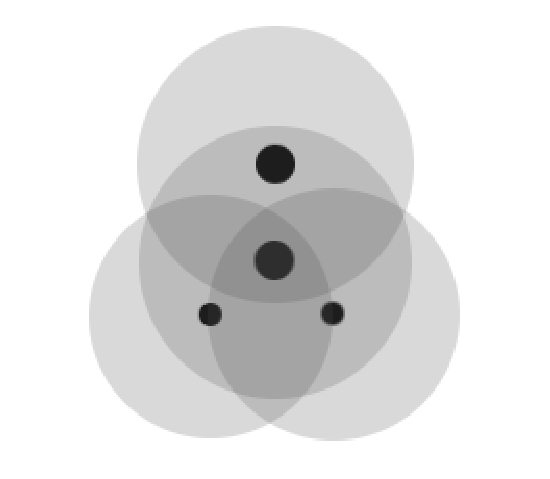
\includegraphics[width=5cm]{03_nevpt/images/rydberg1.eps}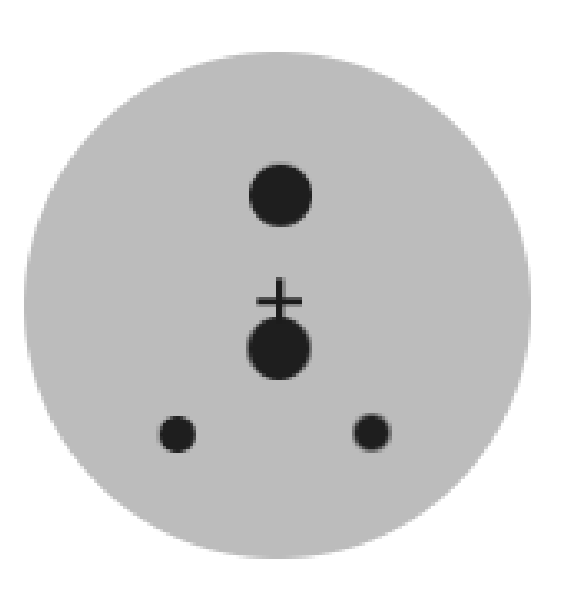
\includegraphics[width=5cm]{03_nevpt/images/rydberg2.eps}
\end{center}
\caption{\footnotesize Two possible schemes to define an augmented basis set
for the description of diffuse Rydberg orbitals: adding diffuse functions on
the single atoms (left side of the picture) or adding diffuse functions
supported by a single dummy atom with no charge. In this thesis, the
development of the Rydberg orbitals followed the second approach.}
\label{fig:rydberg}
\end{figure}
\end{center}


\subsection*{Position of the charge centroid}

The position of the X dummy atom is usually chosen to coincide with the position of
the positive charge centroid, which depends on the molecular geometry and
the excitation performed. Various strategies could be devised in the
evaluation of these coordinates, but practical evaluations performed on
test molecules confirmed the very reduced dependency of the absolute energy
with respect to the dummy atom position. A possible strategy is represented 
by the procedure described by Roos and coworkers\cite{roos-qmescca}.

%A possible strategy is to devise an approximate position by means of the
%dipole $\mu$. For example, in the case of formaldehyde, the higher occupied
%orbitals (by symmetry) for the neutral system are $5a_{1},1b_{1},2b_{2}$.
%The standard geometrical orientation is assumed: the molecule is on the $zy$
%plane, with the carbonyl group along the $z$ axis.  To evaluate the Rydberg
%orbitals for an electronic transition of the type $n_{y} \rightarrow
%\mbox{Ryd}$, an electron is removed from $2b_{2}$. Using the program \dalton
%, a $B_2$ doublet can be evaluated with the following input
%\begin{verbatim}
%**DALTON INPUT
%.RUN WAVE FUNCTION
%.RUN PROPERTIES
%**WAVE FUNCTIONS
%.HF
%*HF INPUT
%.HF OCC
%5 1 1 0
%.MAX DIIS ITERATIONS
%50
%.OPEN SHELL
%3
%**PROPERTIES
%.POPANA
%*END OF INPUT
%\end{verbatim}
%A position for the centroid of the total positive charge can be evaluated
%using the formula
%\beq
%\overrightarrow{R}_{+} = \frac{\sum_{i} e_{+}(i) \overrightarrow{r}_{\! \! +}(i)}{\sum_{i} e_{+}(i)}
%\eeq
%where $i$ runs over the atoms, and $e_{+}(i)$, $\overrightarrow{r}_{\! \! +}(i)$ are
%the nuclear charge and the position of the atom $i$, respectively.
%The same relation could be written for the total negative charge centroid,
%making use of the Mulliken charges
%\beq
%\overrightarrow{R}_{-} = \frac{\sum_{i} e_{-}(i) \overrightarrow{r}_{-}(i)}{\sum_{i} e_{-}(i)}
%\eeq
%but a more accurate value can be obtained using the dipole as provided by \dalton
%\beq
%\overrightarrow{\mu} = \sum_{i} e_{+}(i) \overrightarrow{R}_{+} - \sum_{i} e_{-}(i)
%\overrightarrow{R}_{-}
%\eeq
%Finally, we can obtain the net charge centroid for the ionized molecule
%\beq
%\overrightarrow{R} = \frac{\sum_{i} e_{+}(i) \overrightarrow{R}_{+} + \sum_{i} e_{-}(i)
%\overrightarrow{R}_{-}}{\sum_{i} e_{+}(i) - \sum_{i} e_{-}(i) }
%\eeq
%where the X dummy atom will be placed. 

Another possible strategy is to choose the center of mass. This approach is
simpler, introducing a negligible change in the results, and removes the
need to evaluate the molecular dipole. In the evaluations performed later in
this thesis both approaches have been used, however as already stated
the choice of the position does not produce sizable effects on
the final result.

Once placed, the dummy X atom is provided with an uncontracted basis set.
The exponents for the gaussian functions can be obtained through a
universal algorithm by Kaufmann {\textit et al}\cite{jpb-22-2223-1989}.
\dalton provides an interface to generate these coefficients by means of the
\texttt{.CM FUN} keyword.  The keyword must be provided with three
numbers as defined in Ref. \citen{jpb-22-2223-1989}: the first number
indicates the maximal L quantum number desired for the generated functions.

The second number is related to the starting value for the exponents. The
chosen value gives exponents compatible with small molecules, such as
formaldehyde or acetone.  Kaufmann suggests using a value which provides
exponents in smooth continuity with the core basis set. 

The last number must be equal to or greater than the second, and produces a
new gaussian coefficient for every increment of $\frac{1}{2}$. 

In the performed evaluations the choice (2 2 5.5) has been made.
The first value 2 will generate $s$, $p$ and $d$-type Rydberg diffuse
functions, and the remaining two values 2 and 5.5 produce eight functions.
The final basis set on the X dummy atom is therefore the uncontracted
$8s8p8d$.  Exponents can be extracted from the output file of the \dalton
run.

\subsection*{Contraction of the Rydberg basis set}

The previous section demonstrated how to produce an uncontracted basis set
of diffuse gaussians. These gaussians can be used as-is to enrich the valence
basis set, providing a high number of degrees of freedom in the description of
high-energy Rydberg orbitals, but the resulting basis set is heavily
extended. This introduces a high computational cost and, in the case of
CASPT2 evaluations, convergence problems due to intruder states. 

For these reasons, it is often useful to contract the Rydberg basis set with
appropriate coefficients. A contraction from $8s8p8d$ to $1s1p1d$, for
example, leads to a reduction of the number of additional function from 72
to 9.  A more flexible choice is the contraction to $3s3p3d$, which gives a
good compromise between degrees of freedom and basis set reduction.

An explorative study has been performed to evaluate the influence of Rydberg
contraction on the energy of valence and Rydberg states of formaldehyde.
Tab.~\ref{tbl:rydberg_contraction} reports an evaluation performed on
various excited valence and Rydberg states of the formaldehyde. Details of
the evaluation will be presented in the next section, the only difference
being the basis set, in this case cc-pVTZ\cite{jcp-90-1007-1989}.

As can be seen, the reported values do not change significantly by
decontracting the Rydberg basis set. We can therefore conclude that a
contraction from $8s8p8d$ to $1s1p1d$ is mostly sufficient for obtaining
valuable results.

The procedure to obtain the contraction coefficients has been implemented
\textit{via} both \molcas and \texttt{DALTON}. The \molcas suite provides the \texttt{GENANO}
program, while for the \dalton program an analogous program
\texttt{GENANODAL} has been implemented by our research group.

\begin{center}
\begin{threeparttable}
\footnotesize
\begin{tabular*}{0.70\textwidth}{l@{\hspace{30mm}}cccc}
\hline
                       &  1 Ryd        &  3 Ryd        &  8 Ryd         \\
\hline
                        \multicolumn{4}{c}{\small A$_1$} 	\\
$n_y\!\!\rightarrow\!\! 3p_y$       &   8.14       & 8.14          &  8.14  \\
$n_y\!\!\rightarrow\!\! 3d_{yz}$    &   9.29       & 9.30          &  9.30 \\
$\pi\!\!\rightarrow\!\!\pi^{*}$     &   9.98       & 9.86          &  9.86 \\
                        \multicolumn{4}{c}{\small A$_2$} 	\\
$n_y\!\!\rightarrow\!\!\pi^*$       &   4.05       & 4.03          &  4.04 \\
$n_y\!\!\rightarrow\!\! 3p_x$       &   8.47       & 8.48          &  8.49 \\
$n_y\!\!\rightarrow\!\! 3d_{xz}$    &   9.47       & 9.50          &  9.50 \\
                        \multicolumn{4}{c}{\small B$_2$} 	\\
$n_y\!\!\rightarrow\!\! 3s$               &   7.38       & 7.38          &  7.38 \\
$n_y\!\!\rightarrow\!\! 3p_z$             &   8.29       & 8.24          &  8.24 \\
$n_y\!\!\rightarrow\!\! 3d_{x^2\!-\!y^2}$ &   9.26       & 9.22          &  9.22 \\
$n_y\!\!\rightarrow\!\! 3d_{z^2}$         &   9.43       & 9.39          &  9.39 \\
                        \multicolumn{4}{c}{\small B$_1$} 	\\
$n_y\!\!\rightarrow\!\! 3d_{xy}$          &   9.38       & 9.40          &  9.40 \\
$\sigma\!\!\rightarrow\!\!\pi^{*}$           &   9.37       & 9.33          &  9.33 \\
\hline
\end{tabular*}
\caption{\footnotesize An evaluation of valence and Rydberg excited states transition
energies of formaldehyde, using the cc-pVTZ basis set and different diffuse
basis set contractions. It can be noted that the contraction $8s8p8d$ to
$1s1p1d$ (1 Ryd) produces stable results.\label{tbl:rydberg_contraction}}
\end{threeparttable}
\end{center}


%The theoretical approach is rather simple: a matrix representation of the
%one-particle density matrix must be expressed in the atomic basis set. This
%can be obtained by expressing the one-particle density matrix on a basis set
%of generic spinorbitals $\left\{ \psi_i \left(i\right) \right\}$:
%\beq
%\rho\left(x, x^{\prime}\right) = \sum_{i,j} R_{i,j} \psi_{i} \left( i
%\right) \psi_{j}^{*} \left( x^{\prime} \right)
%\eeq
%Two particular choices of spinorbitals can be defined: the set $\left\{
%\phi_i \left(i\right) \right\}$ of pseudonatural orbitals of a given
%wavefunction and the set of functions used as the atomic basis set $\left\{
%\chi_i \left(i\right) \right\}$. Each one gives the one-particle
%density matrix through a different $R$ matrix
%\beqa
%\rho\left(x, x^{\prime}\right) &=& \sum_{i,j} R^{\mbox{NO}}_{i,j} \phi_{i} \left( i
%\right) \phi_{j}^{*} \left( x^{\prime} \right) \\
%&=& \mathbf{\phi} \mathbf{R}^{NO} \mathbf{\phi} \\
%\rho\left(x, x^{\prime}\right) &=& \sum_{i,j} R^{\mbox{AO}}_{i,j} \chi_{i} \left( i
%\right) \chi_{j}^{*} \left( x^{\prime} \right) \\
%&=& \mathbf{\chi} \mathbf{R}^{AO} \mathbf{\chi} 
%\eeqa
%A matrix of coefficients $\mathbf{C}$ expresses the combination of
%$\mathbf{\chi}$ to obtain $\mathbf{\phi}$
%\beq
%\mathbf{\phi} = \mathbf{\chi} \mathbf{C}
%\eeq
%the $\mathbf{\chi}$ basis set is not orthonormal, since
%\beq
%\mathbf{\chi}^{+}\mathbf{\chi} = \mathbf{S}
%\eeq
%Finally, $\mathbf{R}^{NO}$ is diagonal (given the definition) with
%occupation numbers on the diagonal. In general, the representation
%$R^{\mbox{AO}}$ is not diagonal. The following relation holds:
%\beq
%C^{-1}R^{AO}\left( C^{-1} \right)^{+} = R^{NO}
%\eeq
%Given the following 
%\beq
%\left( C^{-1} \right)^{+} = \left( C^{+} \right)^{-1} = SC
%\eeq
%we obtain
%\beq
%SR^{AO}SC = SCR^{NO}
%\eeq
%Where we obtain the coefficients and eigenvalues of $SR^{AO}S$ in
%a non-unity metric $S$. Once diagonalized, values for the X dummy atom are
%extracted, and a spherical normalization is performed for functions with
%symmetry different from $s$.

\subsection*{Using Molcas}

The procedure using the \molcas suite can be found in the manual
\cite{molcas-site}, and is also reported by Roos et al.\cite{roos-qmescca}.
Here a brief discussion will be presented. The needed steps are:
\begin{itemize}
\item add the diffuse, uncontracted basis set to the molecule (modifying the
\texttt{Seward} input file). The contraction coefficients matrix in this case is a
unit matrix
\item perform a CASSCF evaluation for the system with one electron removed
\item in the resulting output, identify the Rydberg orbitals described by one or
(probably) more functions on the X dummy atom
\item modify the \texttt{.RasOrb} file, containing the orbital coefficients
and their occupation numbers, setting the core occupation numbers to
zero. For the Rydberg orbitals, their occupation numbers must be set
to small, non-zero values, decreasing of one order of magnitude inside each
symmetry. The usual choice is 0.1, 0.01, 0.001 and so on. This prevents
mixing of different Rydberg orbitals inside the same symmetry
\item run the program \texttt{GENANO} with the modified \texttt{RasOrb}
file. This will produce contraction coefficients
\item finally, replace the contraction matrix into the \texttt{Seward} input
file with the new coefficients
\end{itemize}

\subsection*{Using Dalton}

The \dalton suite of programs does not implement a strategy for the
generation of contracted basis sets, therefore an external program has been
developed, named \texttt{GENANODAL}, to accomplish this task. The strategy
is as follows: 
\begin{itemize}
\item perform a Hartree-Fock open shell evaluation for the molecular ion
\item use the program \texttt{IJKLDALI} to perform orbital and integral reordering
\item run the program \texttt{GENANODAL} with an appropriate input, built using the
informations provided by \texttt{IJKLDALI}
\end{itemize}

An example input file is provided:
\begin{verbatim}
&LEGGI FILE11='/scr1/stef/$NAME/FILE11',
       FILE25='/scr1/stef/$NAME/FILE25',
  ZANO=T,NOCCUP=8*0.0,
  0.1,0.01,0.001,0.0001,45*0.0,
  0.0,0.1,0.01,21*0.0,
  0.1,0.01,24*0.0,
  0.1,
  NAOX=72,
  IAOX=23,24,25,26,27,28,29,30,
  64,65,66,67,68,69,70,71,
  92,93,94,95,96,97,98,99,
  31,32,33,34,35,36,37,38,
  39,41,43,45,47,49,51,53,
  40,42,44,46,48,50,52,54,
  72,73,74,75,76,77,78,79,
  100,101,102,103,104,105,106,107,
  111,112,113,114,115,116,117,118,
  MAXL=2,NPRIML=8,8,8,NANOL=1,2,3, &END
\end{verbatim}

\texttt{NOCCUP} have to be set to dummy occupation numbers for each orbital,
honoring the reordering performed by \texttt{IJKLDALI}. As in the case of
\texttt{MOLCAS}, these numbers must be set to values in descending order for the
Rydberg orbitals of the shell we are interested in.

\texttt{NAOX} and \texttt{IAOX} represent how many and which atomic
functions belong to the X dummy atom, repectively. These values must be
extracted from the \texttt{IJKLDALI} output.  The ordering of the functions
must be kept into account: first $s$-type functions, then $p$-type
functions, finally $d$-type functions.

\texttt{MAXL} is the maximal quantum number L to extract. In this case, up to $d$-type
functions are requested.

\texttt{NPRIML} is the number of primitives for each quantum number. For contracting
a $8s8p8d$ Rydberg basis, these values are 8,8,8.

Finally, \texttt{NANOL} are the number of contracted functions generated for each
quantum number L. In this case, provided only as an example, 1 $s$-type
contracted function will be produced, along with 2 $p$-type functions and 3
$d$-type functions. From the output, only the first column of coefficients
will be used.

The \texttt{GENANODAL} code provides exactly the same results as obtained from the
\molcas chain.

%experimental: rydberg della formaldeide e dell'acetone
\section{Evaluation: Rydberg states}

\begin{center}
\textit{This section is based on the article at Ref. \citen{tca-111-352-2004}.}
\end{center}
{\ }\\
\vspace{-1mm}

This section focuses on the description of vertical transitions to valence and
Rydberg excited states with Single-State NEVPT on formaldehyde and acetone.
It aims at completing the detailed description of the excited states of
carbonyl. In the presented evaluation a state-average CASSCF has been
performed. This is different from the previous analysis, where a single state
CASSCF approach was used.

\subsection{Formaldehyde}

The vertical spectrum of the formaldehyde molecule was computed at the
ground state experimental geometry\cite{jms-18-344-1965} (R$_{\mbox{\tiny CO}}$=1.208 \AA,
R$_{\mbox{\tiny CH}}$=1.116 \AA\ and $\theta_{\mbox{\tiny
HCH}}$=116.5$^{\circ}$). As in the previous evaluation, the molecule belongs
to the C$_{2v}$ point group symmetry and lies in the $yz$ plane with the
C and O atoms on the $z$ axis.  The
ANO-1 basis set\cite{tca-77-291-1990} has been used with two different
contraction schemes: the smaller (indicated with ANO(S)) is C,O
[$4s3p1d$]/H[$2s1p$] and the larger (ANO(L)) is C,O
[$6s5p3d2f$]/H[$4s3p2d$].  These valence basis sets have been augmented with
diffuse functions using the procedure described in the previous section, in
order to properly describe the diffuse orbitals involved in the Rydberg
states. These basis functions have been obtained by contraction of a
set of $8s8p8d$ gaussian primitives. Two contraction schemes are considered:
[$1s1p1d$], (Ryd(S)) and [$3s3p3d$], (Ryd(L)).  For a direct comparison
between NEVPT, CASPT2\cite{tca-92-227-1995} and Size-Consistent
Self-Consistent CI ((SC)$^2$-CI)\cite{mp-101-483-2003}, we used in the
calculations the combinations ANO(S)-Ryd(S) and ANO(L)-Ryd(L).

The molecular orbitals are obtained from average CASSCF calculations which
involve the lowest states of a given symmetry. The active spaces, together
with the number and the nature of the states considered in the average
procedure are reported in Tab. \ref{tbl:form_act} and are taken from Ref.
\citen{tca-92-227-1995}.

\input{03_nevpt/tbl_form_act}

The number of orbitals for each irreducible representation
was chosen by the authors so that all the states of interest could be
correctly described. In some cases the active space was enlarged in order
to minimize the effect of the intruder states problem in the CASPT2
calculations.  Given that NEVPT is not affected by the intruder states
problem, in this evaluation a reduction of the active space should be
possible but the comparison of our results with those of Refs.
\citen{tca-92-227-1995} and \citen{mp-101-483-2003} would be in this case less
clear.

The energies of the states are computed in a state specific multireference
perturbation scheme.  The zero-order description of each state is obtained
from a CASCI calculation using the average CASSCF active orbitals. The
inactive orbitals have been canonized to diagonalize the state-specific Fock
matrixes.

A second-order correction to the energy is computed using the NEVPT2 Strongly
Contracted and Partially Contracted variants. All orbitals and
electrons are included in the perturbative treatment. The excitation
energies are computed with respect to the same ground state energy, which is
evaluated as the second order correction to the energy with the reference
energy and wavefunction obtained from a state-specific CASSCF calculation
with four electrons in two $b_1$ ($\pi$ + $\pi^*$) and two $b_2$ ($n_y$ +
virtual) orbitals. This approach for the calculation of the excitation
energies differs from the one used in the CASPT2 calculation, where a
different ground state energy was used for each irreducible representation.

\begin{center}
\begin{threeparttable}
\tiny
\begin{tabular}{lccccccccc}
\hline
Method &2 A$_1$ & 3 A$_1$ & 1 B$_2$ & 2 B$_2$ & 3 B$_2$ & 4 B$_2$ & 2 A$_2$ & 3 A$_2$ &  2 B$_1$ \\
 &($3p_y$) & ($3d_{yz}$) & ($3s$) & ($3p_z$) & 
($3d_{x^2\!-\!y^2}$) & ($3d_{z2}$) & ($3p_x$) &
($3d_{xz}$) & ($3d_{xy}$)     \\
\hline
CASSCF\tnote{a,b}  &   8.07 & 9.18  & 7.37  & 8.15  & 9.08  & 9.21  & 8.84  & 9.78  & 9.16 \\
CASSCF\tnote{a,c}  &   8.04 & 9.12  & 7.29  & 8.08  & 8.99  & 9.12  & 8.81  & 9.72  & 9.12 \\
NEVPT SC\tnote{a,b}&   8.27 & 9.42  & 7.28  & 8.11  & 9.13  & 9.30  & 8.33  & 9.34  & 9.26 \\
                & (0.077)&(0.076)&(0.092)&(0.090)&(0.083)&(0.082)&(0.080)&(0.079)&(0.079)\\
NEVPT SC\tnote{a,c}&   8.39 & 9.56  & 7.32  & 8.16  & 9.17  & 9.37  & 8.46  & 9.48  & 9.39 \\
                & (0.084)&(0.083)&(0.090)&(0.090)&(0.087)&(0.086)&(0.099)&(0.097)&(0.086)\\
NEVPT PC\tnote{a,b}&   8.20 & 9.34  & 7.28  & 8.12  & 9.14  & 9.31  & 8.33  & 9.34  & 9.27 \\
                & (0.084)&(0.084)&(0.095)&(0.093)&(0.085)&(0.084)&(0.082)&(0.081)&(0.081)\\
NEVPT PC\tnote{a,c}&   8.31 & 9.49  & 7.33  & 8.17  & 9.17  & 9.38  & 8.45  & 9.48  & 9.39 \\
                & (0.092)&(0.090)&(0.092)&(0.092)&(0.089)&(0.088)&(0.103)&(0.100)&(0.087)\\
CASPT2 \cite{tca-92-227-1995}
                &   8.12 & 9.24  & 7.30  & 8.09  & 9.13  & 9.31  & 8.32  & 9.31  & 9.23 \\
MC/BMP \cite{cp-205-323-1996}
                &   7.95 & 9.11  & 6.90  & 7.77  & 8.95  & 9.11  & 8.46  & 8.82  & 9.06 \\
(SC)$^2$ CAS+SD\tnote{b} \cite{mp-101-483-2003}
                &   8.14 & 9.26  & 7.17  & 7.96  & 9.00  & 9.19  & 8.30  & 9.28  & 9.12 \\
(SC)$^2$ MR+SD\tnote{c} \cite{mp-101-483-2003}
                &   8.27 & 9.31  & 7.12  & 7.95  & 8.96  & 9.18  & 8.36  & 9.34  & 9.36 \\
CCR(3)$^b$ \cite{mp-101-483-2003}
               &    8.01 & 9.16  & 7.11  & 7.91  & 8.99  & 9.21  & 8.25  & 9.26  & 9.12 \\
CCR(3)$^c$ \cite{mp-101-483-2003}
               &    8.14 & 9.27  & 7.16  & 7.99  & 9.04  & 9.27  & 8.38  & 9.40  & 9.25 \\
MRD-CI \cite{jpc-99-8050-1995}
                &   8.10 & 9.25  & 7.15  & 8.05  & 9.05  & 9.25  & 8.32  & 9.34  & 9.32 \\
MR-CISD + Q \cite{tca-106-369-2001}
                &   8.13 & 9.28  & 7.27  & 8.10  & 9.15  & 9.30  & 8.34  & 9.36  & 9.26 \\
MR-AQCC  \cite{tca-106-369-2001}
                &   8.24 & 9.38  & 7.21  & 8.03  & 9.09  & 9.24  & 8.46  & 9.49  & 9.37 \\
EOM-CCSD \cite{cpl-241-26-1995}
                &   7.99 &10.16  & 6.99  & 7.93  & 9.25  & 9.98  & 8.45  &10.67  & 9.84 \\
EOM-CCSD \cite{jpca-106-4192-2002}
                &   7.98 & 9.13  & 7.04  & 7.88  & 8.94  & 9.12  & 8.21  & 9.29  &10.89 \\
Exp. \cite{robin-hespm}
                &   7.97 &       & 7.11  & 8.14  & 8.88  &       & 8.37  &       &      \\
Exp. \cite{cp-70-291-1982}
                &        &       &       &       &       &       &       &       & 9.22 \\
Exp. \cite{jcsft-281-1643-1985,jcp-85-4228-1986}
                &        &       & 7.09  &       &       &       &       &       &      \\
\hline
\end{tabular}
\caption{\footnotesize Vertical excitation energies (eV) for the Rydberg states of
the formaldehyde molecule.  The numbers in parentheses are the squared norms
of the first order corrections to the wave function. The squared norm for
the ground state is 0.075 (NEVPT SC$^b$), 0.076 (NEVPT PC$^b$), 0.091
(NEVPT SC$^c$) and 0.097 (NEVPT PC$^c$).}
\label{tbl:form_exc_ryd}
\begin{tablenotes}
\footnotesize
\item[a] This work
\item[b] ANO basis set with contraction [$4s3p1d$/$2s1p$] + $1s1p1d$, ANO(S)+Ryd(S)
\item[c] ANO basis set with contraction [$6s5p3d2f$/$4s3p2d$] + $3s3p3d$, ANO(L)+Ryd(L)
\end{tablenotes}
\end{threeparttable}
\end{center}


The vertical excitation energies obtained in our calculations are reported
in Tab. \ref{tbl:form_exc_ryd} for the Rydberg states and in Tab.
\ref{tbl:form_exc_val} for the valence states, together with the previous
theoretical and experimental results.

In Tab. \ref{tbl:form_comparison_1} we show the comparison between our
results and those of Pitarch-Ruiz {\it et al} \cite{mp-101-483-2003}, which
can be considered a good reference since they involve the whole single plus
double excitations space on top of a CAS at a variational level with a
size-consistence correction. We remark that the mean absolute error (MAE) of
our results is always small with the worst case being represented by the
Strongly Contracted NEVPT2 in the ANO(L) + Ryd(L) basis (0.15 eV).  The small
errors appearing in Tab.~\ref{tbl:form_comparison_1} bear out the
reliability of NEVPT2 which can yield results of good accuracy, comparable
with much more refined calculations, but at a reduced computational cost.

For the case of the smaller basis (ANO(S) + Ryd(S)) the CASPT2 results are
also available. NEVPT2 and CASPT2 appear to be of the same quality, with the
former showing in all cases a small squared norm of the wavefunction
perturbation correction thus getting over the intruder states problem.

As to the comparison with the experimental data, beyond a satisfactory
general agreement with our theoretical results we can make the following
observations.

\begin{center}
\begin{threeparttable}
\footnotesize
\begin{tabular*}{0.80\textwidth}{l@{\hspace*{20mm}}ccc}
\hline
Method &4 A$_1$ & 1 A$_2$ & 1 B$_1$ \\
 & (\pipis) & ($n_y\!\!\rightarrow\!\!\pi^*$) & (\sipis) \\
\hline
CASSCF$^{a,b}$          & 10.59  & 5.28  & 9.89  \\
CASSCF$^{a,c}$          & 10.47  & 5.27  & 9.82  \\
NEVPT SC$^{a,b}$        & 10.09  & 4.04  & 9.53  \\
                        & (0.087)&(0.105)&(0.081)\\
NEVPT SC$^{a,c}$        &  9.97  & 3.93  & 9.37  \\
                        & (0.095)&(0.113)&(0.091)\\
NEVPT PC$^{a,b}$        &  9.94  & 4.03  & 9.45  \\
                        & (0.100)&(0.109)&(0.088)\\
NEVPT PC$^{a,c}$        &  9.80  & 3.91  & 9.28  \\
                        & (0.112)&(0.118)&(0.097)\\
CASPT2 \cite{tca-92-227-1995}   &  9.77  & 3.91  & 9.09  \\
MC/BMP \cite{cp-205-323-1996}
                        & 10.37  & 3.83  &13.69  \\ 
(SC)$^2$ CAS+SD$^b$ \cite{mp-101-483-2003}
                        &  9.89  & 4.15  & 9.35  \\
(SC)$^2$ MR+SD$^c$ \cite{mp-101-483-2003}
                        &  9.74  & 4.04  & 9.33  \\
CCR(3)$^b$ \cite{mp-101-483-2003}
                        &  9.80  & 4.01  & 9.29  \\
CCR(3)$^c$ \cite{mp-101-483-2003}
                        &  9.64  & 3.97  & 9.25  \\
MRD-CI \cite{jpc-99-8050-1995}
                        &  9.60  & 4.05  & 9.35  \\
MR-CISD + Q \cite{tca-106-369-2001}
                        &  9.80  & 4.07  & 9.40  \\
MR-AQCC  \cite{tca-106-369-2001}
                        &  9.84  & 4.04  & 9.37  \\
EOM-CCSD \cite{cpl-241-26-1995} &  9.47  & 3.98  & 9.33  \\
EOM-CCSD \cite{jpca-106-4192-2002}&  9.37  & 4.04  & 9.43  \\
Exp. \cite{robin-hespm}      &        & 4.07  &       \\
Exp. \cite{jcp-87-3796-1987}      &        & 3.79  &       \\
\hline
\end{tabular*}
\caption{\footnotesize Vertical excitation energies (eV) for the valence states of
the formaldehyde molecule.  The numbers in parentheses are the squared norms
of the first order corrections to the wavefunction. The squared norm for
the ground state is 0.075 (NEVPT SC$^b$), 0.076 (NEVPT PC$^b$), 0.091
(NEVPT SC$^c$) and 0.097 (NEVPT PC$^c$).}
\label{tbl:form_exc_val}
\begin{tablenotes}
\footnotesize
\item[a] This work
\item[b] ANO(S)+Ryd(S) basis (see text)
\item[c] ANO(L)+Ryd(L) basis (see text)
\end{tablenotes}
\end{threeparttable}
\end{center}


First, in accordance with most theoretical calculations our vertical
2~$^1$A$_1$  and 1~$^1$B$_2$ Rydberg transitions appear in inverted order
with respect to experimental adiabatic transitions \cite{robin-hespm}: a
more stringent comparison would require the calculation of adiabatic
transition with due allowance for the zero point energy correction

Second, the calculation of the $^1$A$_1$ Rydberg states with the larger basis
set introduces one more Rydberg state ($n_y\rightarrow\pi^*$) below the
valence $\pi\rightarrow\pi^*$. Such state has been ignored in the average
CASSCF since we were interested in transitions involving Rydberg orbitals
not exceeding the quantum number $n=3$

Finally, mixing between Rydberg and valence character may occur in both the
$^1$A$_1$ and $^1$B$_1$ transitions \cite{tca-92-227-1995,jpc-99-8050-1995}.
For a correct treatment of such states a quasi-degenerate treatment
is required \cite{acp-67-1-1987,cpl-288-299-1998}.

\begin{center}
\begin{threeparttable}
\footnotesize
\begin{tabular*}{0.80\textwidth}{l@{\hspace*{15mm}}ccc}
\hline
         & NEVPT PC\tnote{a}& NEVPT SC\tnote{a} & CASPT2\tnote{b}    \\
\hline
2 A$_1$  & $~$0.06 & $~$0.13  &    -0.02  \\
3 A$_1$  & $~$0.08 & $~$0.16  &    -0.02  \\
4 A$_1$  & $~$0.05 & $~$0.20  &    -0.12  \\
1 B$_2$  & $~$0.11 & $~$0.11  &  $~$0.13  \\
2 B$_2$  & $~$0.16 & $~$0.15  &  $~$0.13  \\
3 B$_2$  & $~$0.14 & $~$0.13  &  $~$0.13  \\
4 B$_2$  & $~$0.12 & $~$0.11  &  $~$0.12  \\
1 A$_2$  &   -0.12 &   -0.11  &    -0.24  \\
2 A$_2$  & $~$0.03 & $~$0.03  &  $~$0.02  \\
3 A$_2$  & $~$0.06 & $~$0.06  &  $~$0.03  \\
1 B$_1$  & $~$0.10 & $~$0.18  &    -0.26  \\
2 B$_1$  & $~$0.15 & $~$0.14  &  $~$0.11  \\
\hline
MAE\tnote{c}   & $~$0.10 & $~$0.13  &  $~$0.11  \\
\hline
\end{tabular*}
\caption{\footnotesize 
Energy differences (eV) between the perturbation and the (SC)$^2$ CAS+SD
results of Ref. \citen{mp-101-483-2003}
}
\label{tbl:form_comparison_1}
\begin{tablenotes}
\footnotesize
\item[a] This work
\item[b] Ref. \citen{tca-92-227-1995}
\item[c] Mean Absolute Error
\end{tablenotes}
\end{threeparttable}
\end{center}





\subsection{Acetone}

The computational strategy used for acetone closely follows the one applied
to formaldehyde. The vertical spectrum has been computed at the ground
state experimental geometry \cite{jms-18-344-1965}. The molecule belongs to
the C$_{2v}$ point group symmetry with the OCCC skeleton in the $yz$
plane (C and O atoms on the $z$ axis and with an orientation of the CH$_3$ 
groups that place the two H atoms lying in the $yz$ plane as far as
possible). For acetone, we only consider the C,O[$4s3p1d$]/H[$2s1p$]
contraction of the ANO basis set. The Rydberg states are described using a
set of $8s8p8d$ diffuse functions contracted to $1s1p1d$. 

As in formaldehyde, average CASSCF calculations provide the molecular
orbitals: the active spaces and the number and the nature of the states
considered in the average procedure are reported in Tab. \ref{tbl:aceto_act}
and are taken from Ref. \citen{jcp-104-1791-1996}. 

With respect to formaldehyde, the active space has been modified adding the
two CO $\sigma$ and $\sigma^*$ orbitals and the two CO $\sigma$ electrons,
except for the A$_1$ symmetry where three virtual orbitals (one of $b_1$ and
two of $b_2$ symmetry) have been removed. In Ref. \citen{jcp-104-1791-1996}
the CO $\sigma$ and $\sigma^*$ orbitals have been added to the active space
to correctly describe the adiabatic electronic transitions for the
valence states, in which an elongation of the CO bond is observed.
% due to the
% promotion of an electron to the $\pi^{*}$ orbital.

Given that we present here only results on the vertical transitions, also in
the case of acetone a reduction of the active space used in Ref.
\citen{jcp-104-1791-1996} would have been possible, but we have chosen to
maintain the same active space in order to have a meaningful comparison with
the CASPT2 data.

\begin{center}
\begin{threeparttable}
\begin{tabular*}{0.80\textwidth}{clc}
\hline\noalign{\smallskip}
\# MOs \tnote{a} & Symmetry and nature of states    & \# states\tnote{b} \\
\noalign{\smallskip}\hline\noalign{\smallskip}
    (2230)   & $^1$A$_1$ (GS; $n_y\!\rightarrow\! 3p_y$,$3d_{yz}$; $\pi\!\rightarrow\!\pi^*$) & 4 \\
    (2200)   & $^1$B$_1$ ($\sigma\!\rightarrow\!\pi^*$) & 1\\
    (2211)   & $^1$B$_1$ ($n_y\!\rightarrow\! 3d_{xy}$) & 1 \\
    (6210)   & $^1$B$_2$ ($n_y\!\rightarrow\! 3s$, $3p_z$, $3d_{x^2\!-\!y^2}$, $3d_{z^2}$) & 4 \\
    (2410)   & $^1$A$_2$ ($n_y\!\rightarrow\!\pi^*$, $3p_x$, $3d_{xz}$) & 3 \\
\noalign{\smallskip}\hline
\end{tabular*}
\caption{\footnotesize Active spaces and number of states used in the average CASSCF
calculations for the acetone molecule (always 6 active electrons except in
the case of the $^1$B$_1$ ($\sigma\rightarrow\pi^*$) which is computed with
4 active electrons)}
\label{tbl:aceto_act}
\begin{tablenotes}
\footnotesize
\item[a] number of molecular orbitals in the active space for the four
irreducible representations ($a_1$,$b_1$,$b_2$,$a_2$)
\item[b] number of states used in the average procedure
\end{tablenotes}
\end{threeparttable}
\end{center}


The energies of the states are computed following the strategy outlined for
formaldehyde and the transition energies are reported in Tab.
\ref{tbl:aceto_exc_ryd} for the Rydberg states and in Tab.
\ref{tbl:aceto_exc_val} for the valence states, together with the results of
other theoretical calculations and with some experimental results.

We note that our Partially Contracted NEVPT2 results compare very well with
the CASPT2 ones.  We also remark that in two of the valence transitions
(4~$^1$A$_1$, $\pi\rightarrow\pi^*$ and 1~$^1$A$_2$, $n_y\rightarrow\pi^*$)
the difference between Strongly and Partially Contracted NEVPT2 appears to be
unusually sizable (0.59 eV and 0.20 eV, respectively). We think that this is
symptom for the zero-order wavefunction to necessitate significant
improvement.

\begin{center}
\begin{threeparttable}
\tiny
\begin{tabular}{lccccccccc}
\hline
Method &2 A$_1$ & 3 A$_1$ & 1 B$_2$ & 2 B$_2$ & 3 B$_2$ & 4 B$_2$ & 2 A$_2$ & 3 A$_2$ &  2 B$_1$ \\
 &($3p_y$) & ($3d_{yz}$) & ($3s$) & ($3p_z$) & 
($3d_{x^2\!-\!y^2}$) & ($3d_{z2}$) & ($3p_x$) &
($3d_{xz}$) & ($3d_{xy}$)     \\
\hline
CASSCF\tnote{a}  &  7.91  & 8.46  & 6.02  & 6.75  & 7.30  & 7.39  & 7.29  & 7.99  & 7.38  \\
NEVPT2 SC\tnote{a}&  7.40  & 8.03  & 6.75  & 7.67  & 8.25  & 8.37  & 7.48  & 8.24  & 8.36  \\
            & (0.182)&(0.179)&(0.159)&(0.155)&(0.154)&(0.153)&(0.168)&(0.166)&(0.154)\\
NEVPT2 PC\tnote{a}&  7.27  & 7.91  & 6.71  & 7.64  & 8.22  & 8.34  & 7.39  & 8.17  & 8.35  \\
            & (0.195)&(0.192)&(0.166)&(0.161)&(0.160)&(0.158)&(0.177)&(0.175)&(0.158)\\
CASPT2 \cite{jcp-104-1791-1996}
            &  7.26  & 7.91  & 6.58 & 7.48   & 8.04  & 8.18  & 7.34  & 8.09  & 8.20  \\
EOM-CCSD \cite{cpl-241-26-1995}
            &  7.45  & 8.23  & 6.39 & 7.51   & 7.95  & 8.48  & 7.41  & 8.44  & 8.43  \\
EOM-CCSD \cite{jpca-106-4192-2002}
            &  7.41  & 8.02  & 6.42 & 7.39   & 7.82  & 8.10  & 7.31  & 8.04  & 8.11  \\
Exp.\cite{jcp-104-1791-1996}
            &        & 7.8   &      &        & 8.09  &       &       &       & 8.17  \\
Exp.\cite{jcp-98-3795-1993}
            &        &       & 6.35 &        &       &       &       &       &       \\
Exp.\cite{robin-hespm}
            &        &       & 6.36 &        &       &       & 7.45  &       &       \\
Exp.\cite{jcp-89-6086-1988}
            &  7.41  &       &      & 7.45   &       &       & 7.36  &       &       \\
\hline
\end{tabular}
\caption{\footnotesize Vertical excitation energies (eV) for the Rydberg states of
the acetone molecule}
\label{tbl:aceto_exc_ryd}
\begin{tablenotes}
\footnotesize
\item[a] This work. The numbers in parentheses are the squared norms of the
first order corrections to the wavefunction. The squared norm for the
ground state is 0.164 (NEVPT2 SC) and 0.167 (NEVPT2 PC).
\end{tablenotes}
\end{threeparttable}
\end{center}


\begin{center}
\begin{threeparttable}
\footnotesize
\begin{tabular*}{0.80\textwidth}{l@{\hspace*{20mm}}ccc}
\hline
Method &4 A$_1$ & 1 A$_2$ & 1 B$_1$ \\
 & (\pipis) & ($n_y\!\!\rightarrow\!\!\pi^*$) & (\sipis) \\
\noalign{\smallskip}\hline\noalign{\smallskip}
CASSCF\tnote{a}             & 11.60  & 5.57  &10.38 \\
NEVPT2 SC\tnote{a}           &  9.60  & 4.42  & 9.29 \\
                       & (0.204)&(0.189)&(0.182)\\
NEVPT2 PC\tnote{a}           &  9.01  & 4.22  & 9.23 \\
                       & (0.293)&(0.207)&(0.190)\\
CASPT2 \cite{jcp-104-1791-1996}  &  9.16  & 4.18  & 9.10 \\
EOM-CC \cite{cpl-241-26-1995}  &  9.15  & 4.48  & 9.30 \\
EOM-CC \cite{jpca-106-4192-2002} &  8.52  & 4.47  & 8.87 \\
Exp. \cite{jcp-87-3796-1987}     &        & 4.38  &      \\
Exp. \cite{robin-hespm}     &        & 4.43  &      \\
\hline
\end{tabular*}
\caption{\footnotesize Vertical excitation energies (eV) for the valence states of
the acetone molecule}
\label{tbl:aceto_exc_val}
\begin{tablenotes}
\footnotesize
\item[a] This work.  The numbers in parentheses are the squared norms of the
first-order corrections to the wavefunction. The squared norm for the
ground state is 0.164 (NEVPT2 SC) and 0.167 (NEVPT2 PC).
\end{tablenotes}
\end{threeparttable}
\end{center}



\subsection*{Final remarks}

Among the formal requirements satisfied by NEVPT2, the absence of intruder
states appears particularly interesting for the application to the
calculation of electronically excited states. The results shown in the
precedent section for the vertical transitions of formaldehyde and acetone
are of good quality and exhibit good agreements with the best calculations so
far performed as well as with the existing experimental data. 

Our calculations have been carried out starting from rather modest size
CASSCF wavefunctions. The computational overhead involved by the two forms
of NEVPT2 (Strongly and Partially Contracted) amounts to only a small
fraction of the CASSCF calculation for such small active orbital spaces and
this favorable situation is not expected to drastically change when passing
on to larger molecules, provided that the active space can be kept within
manageable dimensions.

No evidence of divergences or misbehaviors in the perturbation summation
has been found in the calculation of the Rydberg states, which are
particularly prone to exhibiting the appearance of intruder states. 

%estensione all'analisi caso qd
\section{Quasi-Degenerate NEVPT2}

Single-State NEVPT2, presented in the previous sections, performs the
perturbative treatment on a given state, disregarding possible interaction
between multiple states which are nearly degenerate before or after the
perturbation. This is due to the definition of a state-specific zero-order
Hamiltonian. To address the needs for quasi-degeneracy problems, frequently
encountered when analyzing avoided crossings, the Quasi-Degenerate NEVPT2
(QD-NEVPT) approach has been implemented\cite{jcp-121-4043-2004}. 

The approach used for NEVPT follows the description made by
Lindgren\cite{jpb-7-2441-1974}.  We define a model space, as generated by a
set of $n$ eigenfunctions, in our case of CASSCF type $\left\{ \Psi_1^{(0)},
\Psi_2^{(0)},\ldots, \Psi_n^{(0)} \right\}$ which undergo altogether the
perturbative correction.  These functions define a space $\mathcal{P}$, and
have associated zero-order energies $E_i^{(0)}$.  We can also define the
complementary space $\mathcal{Q} = 1 - \mathcal{P}$ with
the set of functions $\left\{ \Psi_{n+1}^{(0)}, \Psi_{n+2}^{(0)}, \ldots
\right\}$. Projection operators can be defined for each space
\beqa
\hat{\mathcal{P}} &=& \sum_{i=1}^{n} \ket{\Psi_{i}^{(0)}} \bra{\Psi_{i}^{(0)}} \\
\hat{\mathcal{Q}} &=& \sum_{a > n} \ket{\Psi_{a}^{(0)}} \bra{\Psi_{a}^{(0)}} 
\eeqa
It can be demonstrated that the following relationships hold
\beqa
\label{eqn:qdpt_4}
\hat{\mathcal{P}}^2 = \hat{\mathcal{P}}^{+} = \hat{\mathcal{P}} \\
\hat{\mathcal{P}} \hat{\mathcal{Q}} = \hat{\mathcal{Q}} \hat{\mathcal{P}} = 0 
\eeqa
%\commut{\hat{\mathcal{P}}}{\ham_0} = \commut{\hat{\mathcal{Q}}}{\ham_0} = 0
Defining the true eigenfunctions of the Schr\"odinger equation as
\beq
\ham \Psi_i = E_i \Psi_i
\eeq
we can now write the projection of the true eigenfunctions inside the
spaces defined above
\beqa
\tilde{\Psi}_i &=& \hat{\mathcal{P}} \Psi_i \qquad \forall 1 \le i \le n \\ 
\tilde{\Psi}_a &=& \hat{\mathcal{Q}} \Psi_a \qquad \forall a > n 
\eeqa
and define a ``wave operator'' $\hat{\Omega}$ which produces the true
eigenfunctions $\Psi_i$ from the projected ones
\beq
\hat{\Omega}\tilde{\Psi}_i = \Psi_i 
\eeq
but produces zero when applied to the complementary space
\beq
\hat{\Omega}\tilde{\Psi}_a = 0
\eeq
It can be proved that the following relationships hold
\beqa
\hat{\mathcal{P}} \hat{\Omega} &=& \hat{\mathcal{P}} \\
\hat{\Omega} \hat{\mathcal{P}} &=& \hat{\Omega} \\
\hat{\Omega} \hat{\mathcal{Q}} &=& 0
\eeqa
It is possible to rewrite the Schr\"odinger equation in the form
\beq
\label{eqn:qdpt_2}
\ham \hat{\Omega} \tilde{\Psi}_i = E_i \hat{\Omega} \tilde{\Psi}_i
\eeq
and applying $\hat{\mathcal{P}}$ on both sides
\beqa
\hat{\mathcal{P}} \ham \hat{\Omega} \tilde{\Psi}_i &=& E_i \tilde{\Psi}_i \\
\label{eqn:qdpt_1}
\ham_{\mbox{\tiny eff}} \tilde{\Psi}_i &=& E_i \tilde{\Psi}_i
\eeqa
where an effective Hamiltonian $\ham_{\mbox{\tiny eff}} = \hat{\mathcal{P}} \ham
\hat{\Omega}$ has been defined.  This Hamiltonian produces the eigenvalues
$E_i$ of the true Hamiltonian, but operates in the model space.


The final goal of this technique is to obtain the matrix
$\braket{\Psi_n^{(0)}}{\ham_{\mbox{\tiny eff}}}{\Psi_m^{(0)}}$ and diagonalize it.
This matrix has the dimensionality of the number of states considered in the
Quasi-Degenerate scheme. Once diagonalized, it provides the corrected
energies and the coefficients mixing the perturbed wavefunctions.

To accomplish this task, further elaborations are needed: making use of
Eqn.~\ref{eqn:qdpt_1} by applying on both sides
$\hat{\Omega}$ and subtracting \ref{eqn:qdpt_2} we obtain
\beq
\left( \hat{\Omega} \ham_{\mbox{\tiny eff}} - \ham \hat{\Omega} \right)
\tilde{\Psi}_i = 0
\eeq
which is valid also for $\tilde{\Psi}_a$, therefore the operator itself is
zero
\beq
\hat{\Omega} \ham_{\mbox{\tiny eff}} - \ham \hat{\Omega} = 0
\eeq
Replacing the definition of $\ham_{\mbox{eff}}$ we obtain the
generalized Bloch equation
\beq
\hat{\Omega} \hat{\mathcal{P}} \ham \hat{\Omega} - \ham \hat{\Omega} = 0
\eeq

Introducing the expression of the Hamiltonian as $\ham = \ham_0 + \hat{V}$
we can now perform a substitution inside the Bloch equation to obtain 
\beq
\commut{\hat{\Omega}}{\ham_0} = \hat{\mathcal{Q}} \hat{V} \hat{\Omega} -
\hat{\mathcal{Q}} \hat{\Omega} \hat{\mathcal{P}} \hat{V} \hat{\Omega}
\eeq
To proceed further in the development, a perturbative expansion for the wave
operator and the effective Hamiltonian is performed
\beq
\hat{\Omega} = \hat{\mathcal{P}} + \hat{\Omega}^{(1)} + \hat{\Omega}^{(2)} + \dots
\eeq
and the following relationships can be obtained
\beqa
\commut{\hat{\Omega}^{(1)}}{\ham_0} &=& \hat{\mathcal{Q}} \hat{V}
\hat{\mathcal{P}} \label{eqn:qdpt_6}\\
\commut{\hat{\Omega}^{(2)}}{\ham_0} &=& \hat{\mathcal{Q}} \hat{V}
\hat{\Omega}^{(1)} - \hat{\mathcal{Q}} \hat{\Omega}^{(1)} \hat{\mathcal{P}}
\hat{V} \hat{\mathcal{P}} \\
&\vdots& \nonumber
\eeqa 

Applying the commutator in \ref{eqn:qdpt_6} to $\ket{\Psi_i}$ and
keeping into account that $\hat{\mathcal{Q}} \hat{\Omega}^{(1)} =
\hat{\Omega}^{(1)}$ we obtain
\beq
\left( E_i^{(0)} - \hat{\mathcal{Q}} \ham_0 \hat{\mathcal{Q}} \right)
\hat{\Omega}^{(1)} \ket{\Psi_i} = \hat{\mathcal{Q}} \hat{V} \ket{\Psi_i}
\eeq
which can be rearranged to produce
\beq
\hat{\Omega}^{(1)} \ket{\Psi_i^{(0)}} = \left( E_i^{(0)} - \hat{\mathcal{Q}}
\ham_0 \hat{\mathcal{Q}} \right)^{-1} \hat{\mathcal{Q}} \hat{V}
\ket{\Psi_i^{(0)}}
\eeq
and knowing that
\beq
\hat{\mathcal{Q}} \ham_0 \hat{\mathcal{Q}} = \sum_{a} \ket{\Psi_a^{(0)}}
E_a^{(0)} \bra{\Psi_a^{(0)}}
\eeq
we obtain
\beq
\hat{\Omega}^{(1)} \ket{\Psi_i^{(0)}} = \sum_{a > n} \ket{\Psi_a^{(0)}}
\frac{\braket{\Psi_a^{(0)}}{\hat{V}}{\Psi_i^{(0)}}}{E_i^{(0)} - E_a^{(0)}}
\eeq

We can now apply the perturbative expansion also to $\ham_{\mbox{\tiny eff}}$
\beq
\ham_{\mbox{\tiny eff}} =  \ham_{\mbox{\tiny eff}}^{(0)} + \ham_{\mbox{\tiny
eff}}^{(1)} + \ham_{\mbox{\tiny eff}}^{(2)} + \dots
\eeq
to obtain the following terms
\beqa
\ham_{\mbox{\tiny eff}}^{(0)} &=& \hat{\mathcal{P}} \ham^{(0)} \hat{\mathcal{P}} \\
\ham_{\mbox{\tiny eff}}^{(1)} &=& \hat{\mathcal{P}} \hat{V} \hat{\mathcal{P}} = 0 \\
\ham_{\mbox{\tiny eff}}^{(2)} &=& \hat{\mathcal{P}} \hat{V} \hat{\Omega}^{(1)}  \\
&\vdots&
\eeqa
hence, the $\mathbf{H}_{\mbox{\tiny eff}}$ matrix up to the second-order
can be obtained from the formulation of the $\ham_{\mbox{\tiny eff}}^{(2)}$ operator. 

When applying the above formulations to the NEVPT case, we have to consider
that the model space is generated by the CAS wavefunctions $\left\{
\Psi_m^{(0)} \right\}$, and the zero-order Hamiltonian is defined through its
spectral decomposition
\beqa
\ham_0(m) &=& \ket{\Psi_m^{(0)}} E_m^{(0)} \bra{\Psi_m^{(0)}} \\
&&+ \sum_{m^{\prime} \neq m} \ket{\Psi_{m^{\prime}}^{(0)}} E_{m^{\prime}}^{(0)}
\bra{\Psi_{m^{\prime}}^{(0)}} \\
&&+ \sum_{l,k,\mu} \ket{\Psi_{l,\mu}^{k}(m)} E_{l,\mu}^{k}(m)
\bra{\Psi_{l,\mu}^{k}(m)}
\eeqa
where $\Psi_{l,\mu}^{k}(m)$ are the perturbers generated by the
application of excitation operators to the state $m$. As a consequence, the
zero-order Hamiltonian is state dependen. A partition of the Hamiltonian in
a state-specific way is needed using the multipartitioning
approach\cite{cpl-233-597-1995}. For each state $m$ we define a different
partitioning scheme of the Hamiltonian
\beq
\ham = \ham_0(m) + \hat{V}(m) 
\eeq
It must be noted however that both spaces $\mathcal{P}$ and $\mathcal{Q}$
(and consequently the projection operators) are not state-specific, since
$\mathcal{P}$ is defined by the CAS space, and $\mathcal{Q} = 1 -
\mathcal{P}$. We obtain for $\hat{\Omega}^{(1)}$
\beq
\hat{\Omega}^{(1)} \ket{\Psi_m^{(0)}} = \sum_{k,l,\mu}
\frac{\ket{\Psi_{l,\mu}^{k}(m)}
\braket{\Psi_{l,\mu}^{k}(m)}{\ham}{\Psi_{m}^{(0)}}}{E_m^{(0)} -
E_{l,\mu}^{k}(m)}
\eeq
and the final $\ham_{\mbox{\tiny eff}}$ matrix element is therefore
\beq
\braket{\Psi_n^{(0)}}{\ham_{\mbox{\tiny eff}}}{\Psi_m^{(0)}} = \delta_{nm}
E_m^{(0)} + \sum_{l,k,\mu}
\frac{\braket{\Psi_n^{(0)}}{\ham}{\Psi_{l,\mu}^{k}(m)}
\braket{\Psi_{l,\mu}^{k}(m)}{\ham}{\Psi_m^{(0)}}}{E_m^{(0)} -
E_{l,\mu}^{k}(m)}
\eeq

It can be noted that the diagonal elements of the obtained matrix are the
single state contributions. In a Single-State approach, the non-diagonal
elements of the effective matrix are assumed as zero. The Quasi-Degenerate
approach provides these non-diagonal elements, whose role is to mix the
perturbed wavefunctions.

The $\mathbf{H}_{\mbox{\tiny eff}}$ matrix in general is not hermitian, but a
hermitian variant can be obtained\cite{np-20-321-1960}:
\beq
\mathbf{H}_{\mbox{\tiny eff}}^{\prime} = \mathbf{S}^{-\frac{1}{2}}
\mathbf{H}_{\mbox{\tiny eff}} \mathbf{S}^{\frac{1}{2}}
\eeq
with $S_{ij} = \integral{\tilde{\Psi}_i}{\tilde{\Psi}_j}$.


%procedura sperimentale qdpt
\section{Evaluation: QDPT on formaldehyde}

\begin{center}
\textit{This section is based on the article at Ref. \citen{ijqc-2005}} \\
\end{center}
{\ }\\
\vspace{-5mm}

A Quasi-Degenerate NEVPT2 evaluation has been conducted over the
formaldehyde molecule. Four electronic states of A$_1$ symmetry have been
considered in the analysis, namely the ground state (1A$_1$), the $n_y \rightarrow
3p_y$ Rydberg state (2A$_1$), the $n_y \rightarrow 3d_{yz}$ Rydberg state
(3A$_1$) and the $\pi \rightarrow \pi^{*}$ valence state (4A$_1$). 

The energy curves for these states have been studied as a function of the CO
distance. The rationale behind this study is to analyze the qualitative
behavior of the avoided crossing of the potential energy curves arising from
these states.  A simple CASSCF wavefunction does not keep fully into account
the dynamic correlation needed for the description of the ground and $\pi
\rightarrow \pi^{*}$ state. These states require higher correlative
corrections than the ones needed by the Rydberg states, due to the high
average distance of the promoted electron from the molecular framework in
the Rydberg case.  Also, the large mixing occurring between Rydberg and
valence states invokes the need for a Quasi-Degenerate treatment.

A state averaged CASSCF procedure with an active space of six electrons in
seven orbitals has been performed. The interested active orbitals are the
$\sigma$, $\sigma^{*}$, the $\pi$, $\pi^{*}$, the $n_y$ and the $3p_y$ and
$3d_{yz}$ Rydberg orbitals. To describe the potential curve, CO bond
distances from 2.00 bohr to 3.40 bohr have been considered, with a step of
0.1 bohr.  Occasionally, the step length has been reduced to address
particular features of the curves. Other geometrical parameters have been
kept fixed at the values obtained by a HF/MP2 complete optimization with
the same basis set.

The basis set is the ANO-1, augmented with a Rydberg set of functions built
as detailed in Sec. \ref{sec:rydberg_procedure}. The contraction scheme
produced a set [$1s1p1d$] from a decontracted set of diffuse functions
[$8s8p8d$], centered on the charge centroid evaluated at the ground state
geometry. The position of the centroid is unchanged during the CO
elongation, given its marginal influence on the final results.

The procedure is briefly presented here: for each molecular geometry an
averaged CASSCF evaluation has been performed, producing a set of averaged
molecular orbitals. For each state, the average orbitals are brought in
canonical form in the inactive set. 

\begin{center}
\begin{figure}[ht]
\begin{center}
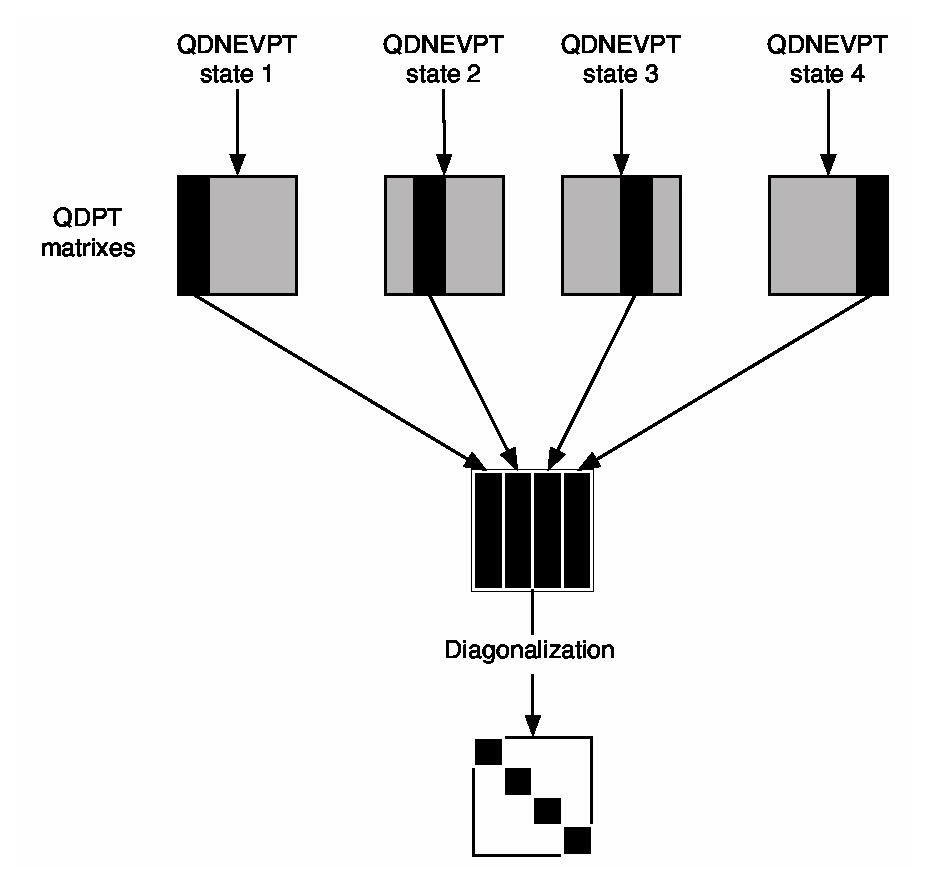
\includegraphics[width=10cm]{03_nevpt/images/qdpt_diagram-gimped.eps}
\end{center}
\caption{\footnotesize The computational scheme for the evaluation of the
Quasi Degenerate treatment. Four different QDPT matrixes are obtained by the
procedure, each one referring to a particular state. A single column is
extracted from each matrix and gathered in a final matrix which is
diagonalized. }
\label{fig:qdpt_diagram}
\end{figure}
\end{center}


This procedure provides four orbital sets, which are used in the Quasi-Degenerate evaluation. Four matrixes are obtained (refer to Fig.
\ref{fig:qdpt_diagram}) each one referring to a particular state. To build
the final effective Hamiltonian matrix to be diagonalized, the following
steps must be applied:
\begin{enumerate}
\item decompose the four matrixes columnwise
\item extract the column number $n$ from the matrix referring to the $n$-th
electronic state
%\item check if coupling (non-diagonal) elements have the correct sign
\item build a final matrix, made of the obtained columns
\item diagonalize it to obtain the final energies and coefficients
\end{enumerate}

%Some explanation have to be reported for the third point: non-diagonal
%elements refer to integrals
%$\braket{\Psi_n^{(0)}}{\ham_{\mbox{eff}}}{\Psi_m^{(0)}}$. The computational
%procedure followed by each matrix is the same, but the final wavefunctions
%can differ in sign. As an example, in the evaluation of the first state the
%element $\braket{\Psi_2^{(0)}}{\ham_{\mbox{eff}}}{\Psi_1^{(0)}}$ can be
%referred to wavefunction with the same sign. For the evaluation of
%$\braket{\Psi_1^{(0)}}{\ham_{\mbox{eff}}}{\Psi_2^{(0)}}$, the sign of
%$\Psi_2^{(0)}$ can be different. A direct comparison of the two integrals is
%not possible, due to their different absolute values.

%A possible solution is to choose as a reference the evaluation matrix provided
%by the first electronic state.  Orbitals for the remaining states are
%preserved only in the inactive part, while the active part is replaced with
%the orbitals from the first set. This approach is formally correct since the
%CAS evaluation is a Full-CI inside this orbital space, and the NEVPT
%treatment is invariant for orbital mixing inside the active block. A quick
%check for the sign of the CI coefficients now can be performed, an
%appropriate sign adaptation for each element of the final matrix. The
%procedure has been implemented as an automatic bash script to prevent
%errors from a manual process.

The curves obtained at CASSCF level are represented in Fig.
\ref{fig:formaldehyde_cas_curve}. The main feature is the behavior of the
$\pi \rightarrow \pi^{*}$ 4A$_1$ state with respect to 2A$_1$ and 3A$_1$
Rydberg states. The Rydberg states are nearly parallel to the ground state.
This is expected since the electron is promoted from a non-bonding orbital
to a distant one, introducing very little destabilization in the electronic
asset that governs the molecular geometry.

On the other hand, the valence
excited state introduces a serious variation in this asset, moving from a
double bond situation to a nearly single bond situation. This imposes a
steep elongation of the bond, and the potential energy curve for this state
crosses the Rydberg ones. Due to interaction between these states, an
avoided crossing situation occurs, producing the resulting diagram.
\vspace{-3mm}
\begin{center}
\begin{figure}[ht]
\begin{center}
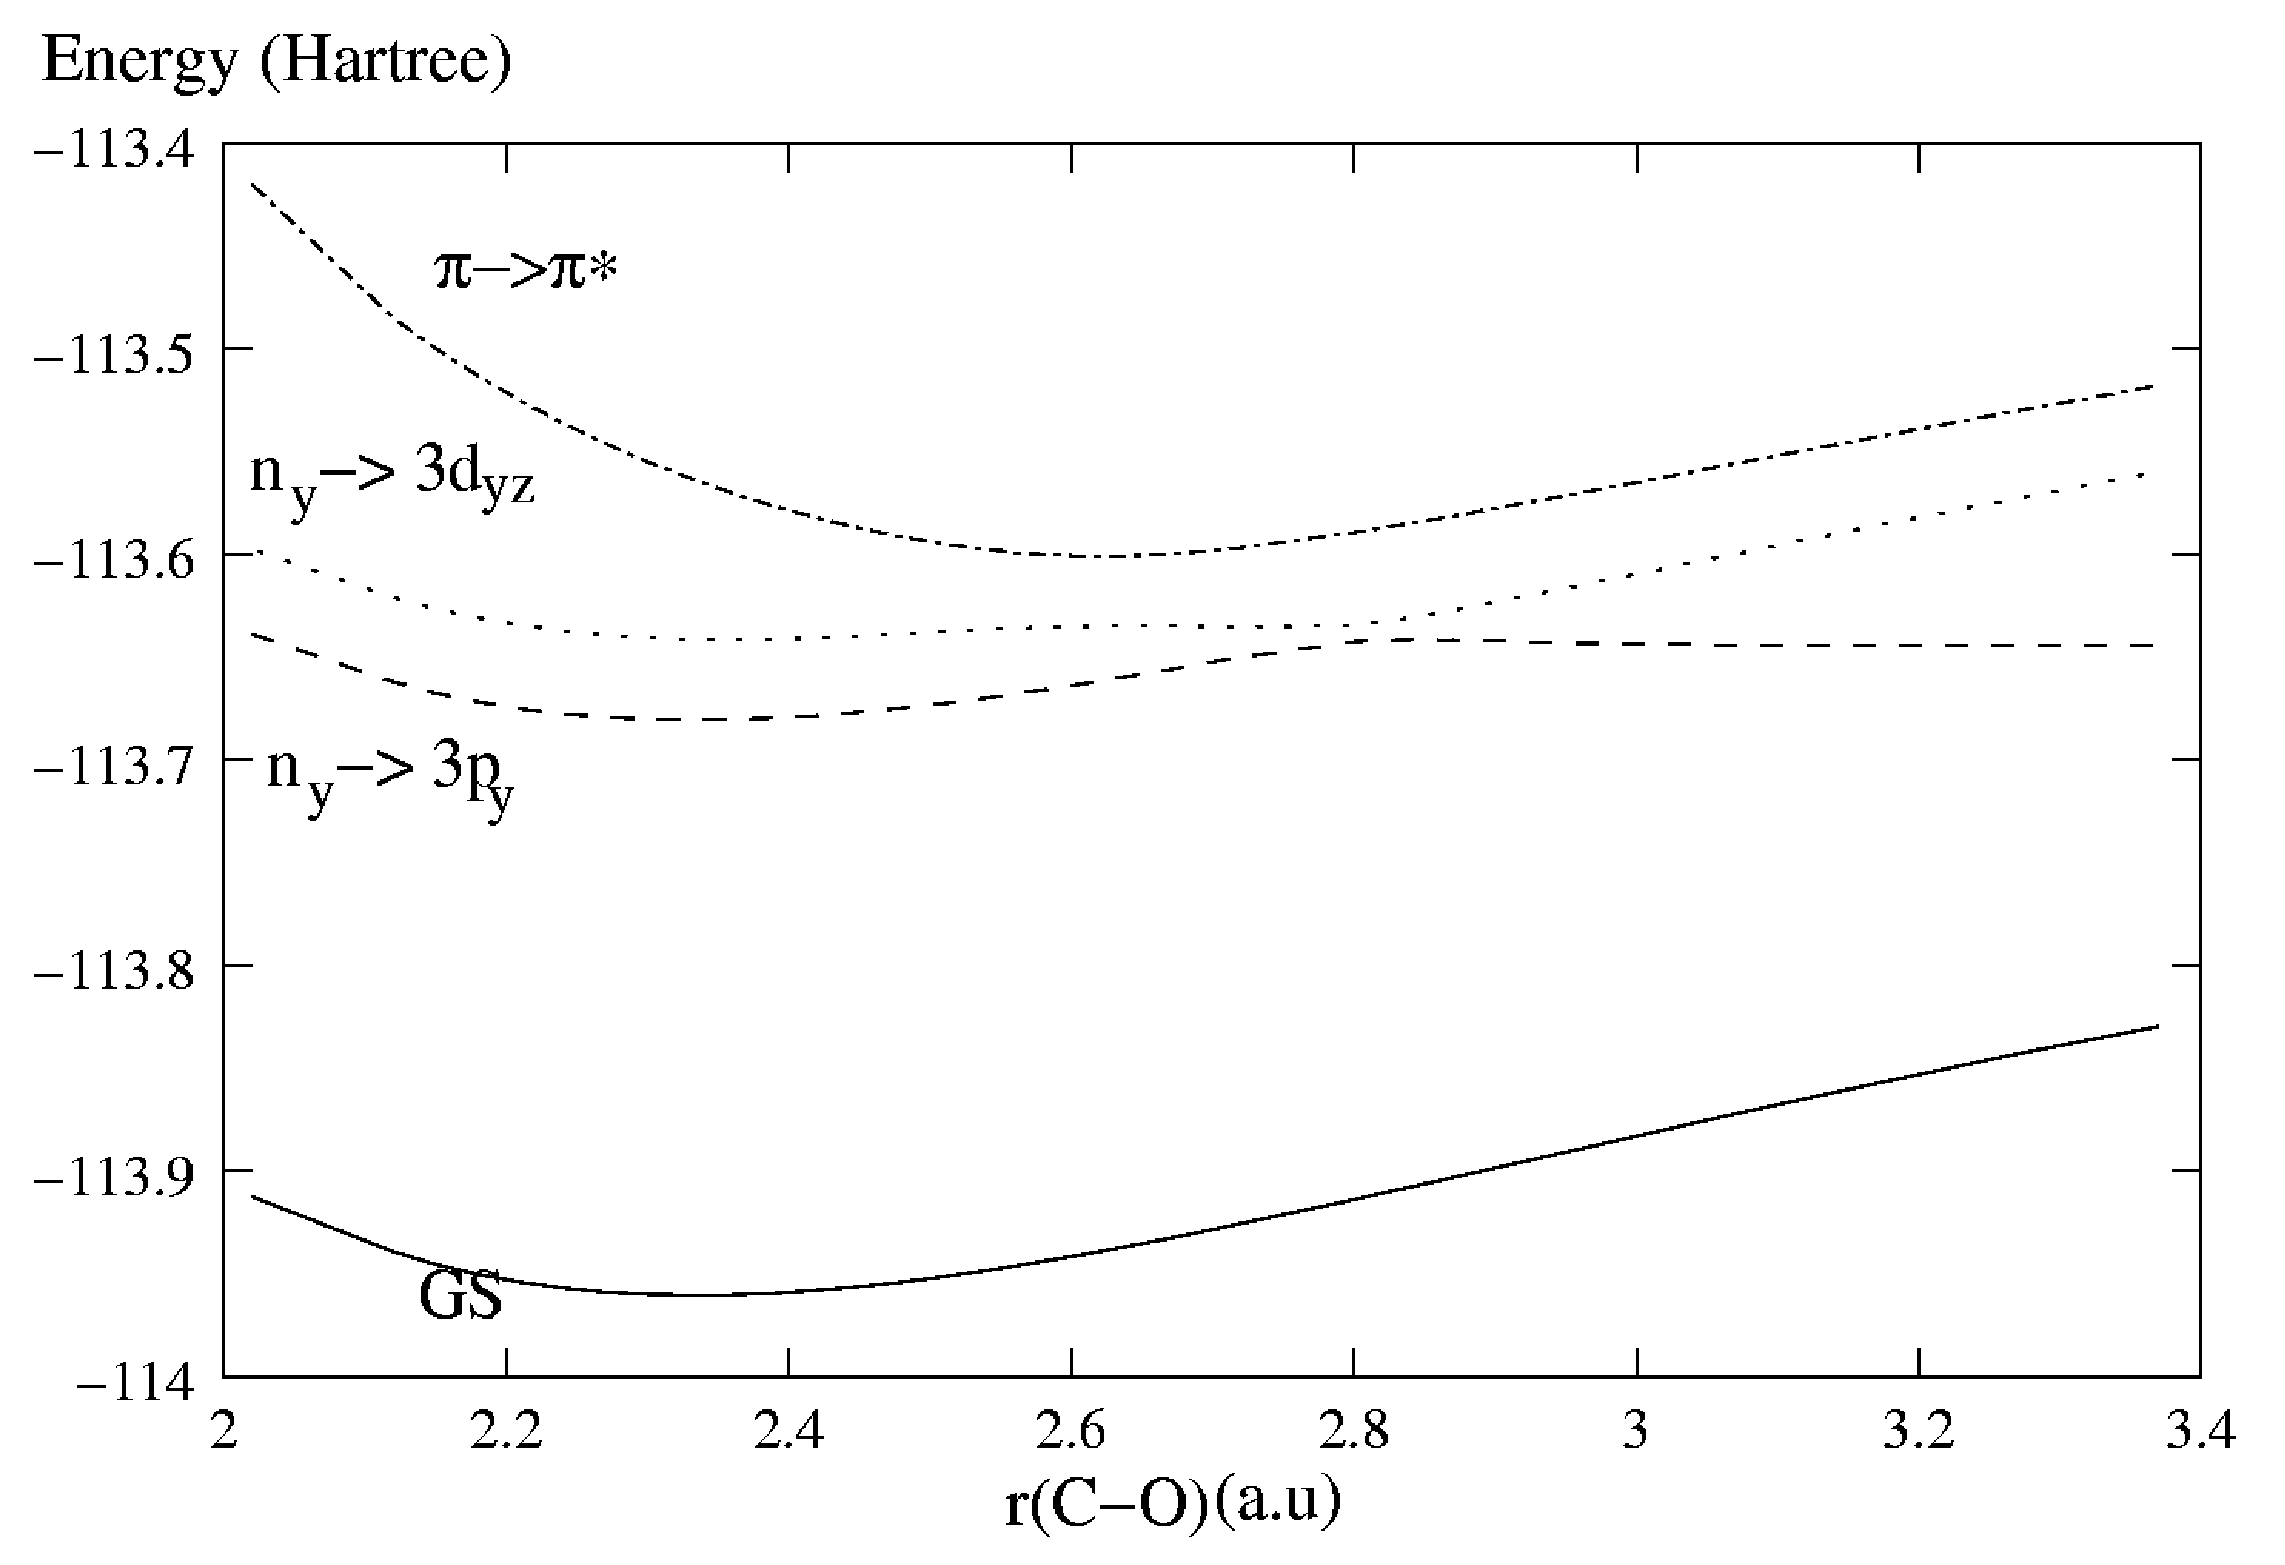
\includegraphics[width=11cm,keepaspectratio]{03_nevpt/images/formaldehyde-cas-curve.eps}
\end{center}
\caption{\footnotesize CASSCF energy curves for the ground state, $n \rightarrow$
Rydberg and $\pi \rightarrow \pi^{*}$ of formaldehyde with respect to the CO
bond lenght.}
\label{fig:formaldehyde_cas_curve}
\end{figure}
\end{center}

Applying the perturbation treatment, it is expected that the correlation for
valence states will be higher than for Rydberg states. 
As a direct consequence the avoided crossings move at shorter distances, see
Fig.~\ref{fig:formaldehyde_qdpt_curve}, solid line. The same plot also
reports the results produced by a Single-State NEVPT2 treatment (dotted
lines). These curves have no physical meaning and behave in incorrect ways.
The presence of non-diagonal elements in the effective Hamiltonian matrix
fixes the invalid behavior, allowing the wavefunction to interact at NEVPT2
level.
\vspace{-3mm}
\begin{center}
\begin{figure}[ht]
\begin{center}
\includegraphics[width=11cm]{03_nevpt/images/formaldehyde-qdpt-curve.eps}
\end{center}
\caption{\footnotesize Energy curves for the ground state, $n \rightarrow$
Ryd and $\pi \rightarrow \pi^{*}$ of formaldehyde with respect to the CO
bond lenght. The solid line represents the QD-NEVPT evaluation. The dotted
lines report the Single-State evaluation.}
\label{fig:formaldehyde_qdpt_curve}
\end{figure}
\end{center}

\vspace{-3mm}
A final consideration must however be raised working with a more accurate
point grid. The plot in Fig. \ref{fig:qdpt_error} represents the 2A$_1$ and
3A$_1$ Rydberg states at QD-NEVPT level of theory, using a finer grid (step
0.01 bohr) between 2.7 bohr and 2.9 bohr. An incorrect behavior is observed
for both curves. This behavior is not appreciable in the Ground
State and $\pi \rightarrow \pi^{*}$ curves. For comparison, the avoided
crossing at CASSCF level is reported between the QDPT curves. The CASSCF
curves have been transposed in energy to fit correctly into the plot.

It can be noted that the position of the incorrect behavior matches the
position of the avoided crossings at CASSCF level. This is probably due to a
wrong estimation of the coupling between the curves. Tests performed with
larger CAS spaces lead to a reduction of the incorrect behavior, which
expresses itself at shorter distances, following again the avoided crossing.
A possible explanation of the problem lies in a bad description of the
zero-order situation, and the inability for the NEVPT2 treatment to fully
recover the coupling. This brings a ``memory-effect'' on the QDPT curves.  A
non trivial solution to the problem could be looked for in the definition of an
iterative procedure, where the QD-NEVPT treatment is performed on the
refined wavefunctions obtained from the previous step. 
\vspace{-3mm}
\begin{center}
\begin{figure}[ht]
\begin{center}
\includegraphics[width=7cm,keepaspectratio,angle=270]{03_nevpt/images/qdpt_error.eps}
\end{center}
\caption{\footnotesize The incorrect behavior of the 2A$_1$ (cross symbol)
and 3A$_1$ (star symbol) Rydberg states at QD-NEVPT level, with respect to
the elongation of the CO bond. A grid step of 0.01 bohr between 2.7 and 2.9
bohr has been used.
Between the curves the plot also depicts the CASSCF avoided crossing taking
place at the same bond length. The avoided crossing curves have been
transposed to better fit into the plot. } \label{fig:qdpt_error}
\end{figure}
\end{center}

\vspace{-6mm}


%non canonical
\section{Non Canonical NEVPT}

All the cases so far examined of NEVPT were performed assuming canonical
orbitals, since the situation is greatly simplified using these orbitals.
Let us consider the inactive part of the Dyall's Hamiltonian in generalized form
\beqa
\ham^D_i &=& \sumidx{ij} f_{ij} E_{ij} + \sumidx{rs} f_{rs} E_{rs}
\eeqa
where the $f_{xy}$ elements are relative to the Fock matrix on a CASSCF
wavefunction $\Psi_0$
%\beq
%f_{xy} = \half \sum_{\sigma=\alpha,\beta}
%\braket{\Psi_0}{\anticomm{\constr{y\sigma}}{\comm{\destr{x\sigma}}{\ham}}
%}{\Psi_0}
%\eeq
\beq
f_{xy} = - \braket{\Psi_0}{\constr{x} \comm{\ham}{\destr{y}}}{\Psi_0} +
\braket{\Psi_0}{\destr{x} \comm{\ham}{\constr{y}}}{\Psi_0}
\eeq
Diagonalization of $\ham^D$ is simplified if we assume that
canonical orbitals are used and the inactive part is cast as the
well-known diagonal case
\beqa
\ham^D_i &=& \sumidx{i} \epsilon_{i} E_{ii} + \sumidx{r} \epsilon_{r} E_{rr}
\eeqa
The simplification arises by the fact that the perturber energies are
defined by a simple quantity. For example, we recall the case for the S$^0$
class where the energy of the perturber $E_{ri} E_{sj} \Psi_m^{(0)}$ is
$E_m^{(0)} + \epsilon_r + \epsilon_s - \epsilon_i -\epsilon_j$. This
obviously cannot be obtained quickly if non-canonical orbitals are used.

A solution resides in a different evolution of the first-order perturbation
equation:
\beq
\left( \ham^{(0)} - E_m^{(0)} \right) \Psi_m^{(1)} = \left( E_m^{(1)} - \hat{V} \right) \Psi_m^{(0)}
\eeq
Instead of expressing the $\Psi_m^{(1)}$ as a linear combination of the
zero-order wavefunctions
\beq
\Psi_m^{(1)} = \sumidx{k}c_k \Psi_k^{(0)}
\eeq
we develop using generic functions $\Phi_l$
\beq
\Psi_m^{(1)} = \sumidx{l}c_l \Phi_l
\eeq
A system of linear equations must be solved
\beq
\sum_l c_l \left[ \braket{\Phi_k}{\ham_0}{\Phi_l} - E_m^{(0)}
\integral{\Phi_k}{\Phi_l} \right] = - \braket{\Phi_k}{\hat{V}}{\Psi_m^{(0)}}
\eeq
\beq
E_m^{(2)} = \braket{\Psi_m^{(0)}}{\hat{V}}{\Psi_m^{(1)}} = \sum_l c_l
\braket{\Psi_m^{(0)}}{\hat{V}}{\Phi_l}
\eeq
using the internally contracted $E_{wx} E_{yz} \Psi_m^{(0)}$ as $\Phi_l$.

%Once deployed the linear system of equations, it can be cast in the form
%\beq
%\left(\mathbf{1} - \mathbf{A} \right) \mathbf{x} = \mathbf{x}_0
%\eeq
%FIXME : spiegare i simboli
%and solved iteratively by building a set of vectors $\mathbf{x}_0$,
%$\mathbf{x}_1$, $\ldots$, $\mathbf{x}_k$ given by
%\beq
%\mathbf{x}_{n+1} = \mathbf{A} \mathbf{x}_{n} - \sum_{l=0,n}
%\frac{\braket{\mathbf{x}_{l}}{A}{\mathbf{x}_{n}}}{\integral{\mathbf{x}_{l}}{\mathbf{x}_{l}}}
%\mathbf{x}_{l}
%\eeq
%It is now possible to optimize the $\alpha_k$ coefficients of the vector
%$\mathbf{x} = \sum_k \alpha_k \mathbf{x}_{k}$ by minimizing the square norm
%of the error vector
%\beq
%\integral{\left(\mathbf{1} - \mathbf{A} \right) \mathbf{x} -
%\mathbf{x}_0}{\left(\mathbf{1} - \mathbf{A} \right) \mathbf{x} -
%\mathbf{x}_0}
%\eeq

\section{NEVPT and Localization}

A first successful integration of localization and NEVPT2 has been deployed
to show the feasibility of this approach.
An acetone molecule and two water molecules coordinating the CO oxygen have
been optimized at 6-311G*/MP2 level. The molecular system has C$_{2v}$
geometrical symmetry, and the CH$_3$ groups have been rotated to feature
on-plane hydrogens far from one another. The symmetry has been considered
only during geometry optimization, while for the rest of the evaluation the
C$_1$ symmetry group has been used to work with non-symmetric localized
orbitals.

A minimal atomic basis set ANO-1 with $2s1p$ contraction for heavy atoms, and
$1s$ for hydrogen has been used. From this basis, a set of localized orbitals
is obtained with the procedure presented in Sec.
\ref{sec:toulouse_method}. These orbitals are optimized by means of a
Super-CI based optimization chain, converging to a localized CASSCF
solution. An active space comprising six electrons in five
active orbitals ($\sigma$, $\sigma^{*}$, $\pi$, $\pi^{*}$ of the acetone
carbonyl group, and the $n_y$ lone pair of the carbonyl oxygen) has been
defined. The active orbitals are visible in Fig. \ref{fig:h2o-active}

\begin{center}
\begin{figure}[ht]
\begin{center}
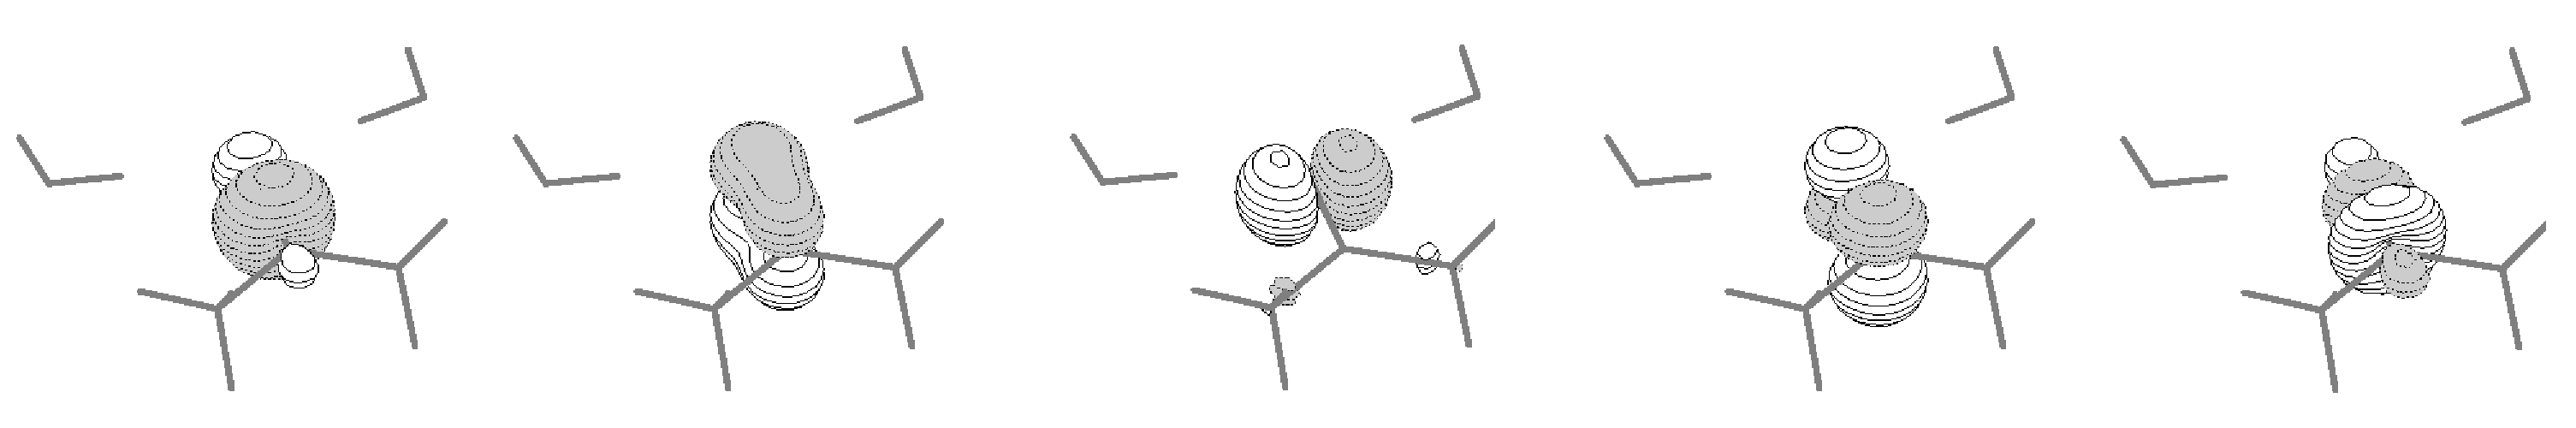
\includegraphics[width=11cm]{03_nevpt/images/h2o-active.eps}
\end{center}
\caption{\footnotesize The active orbitals for the evaluation on Acetone + 2
H$_2$O. From left to right, the $\sigma$, $\pi$, $n_y$, $\pi^{*}$,
$\sigma^{*}$. }
\label{fig:h2o-active}
\end{figure}
\end{center}


These orbitals are used in a Single-State NEVPT2 and a Non-Canonical
procedure, leading to the perturbative results presented in the left side
of Tab.~\ref{tbl:noncanonical}.  

\begin{center}
\begin{threeparttable}
\footnotesize
\begin{tabular*}{\textwidth}{l@{\hspace*{27mm}}cccc}
\hline
        & \multicolumn{2}{c}{Non-canonized} & \multicolumn{2}{c}{Canonized} \\
        &  SS-NEVPT     &  NC-NEVPT     &  SS-NEVPT     &  NC-NEVPT     \\
\hline
        &    \multicolumn{4}{c}{Ground State}\\
  (0)   & -0.1562219292 & -0.1610160883 & -0.1610160655 & -0.1610160655 \\
  (+1)  & -0.0060289124 & -0.0063728566 & -0.0063728572 & -0.0063728572 \\
  (-1)  & -0.0083210019 & -0.0084680922 & -0.0084680918 & -0.0084680918 \\
  (+2)  & -0.0021959738 & -0.0022262691 & -0.0022262691 & -0.0022262691 \\
  (-2)  & -0.0012134175 & -0.0011964952 & -0.0011964953 & -0.0011964954 \\
  (+1)' & -0.0011298902 & -0.0010747735 & -0.0010747734 & -0.0010747734 \\
  (-1)' & -0.0081324857 & -0.0080043857 & -0.0080043841 & -0.0080043842 \\
  (0)'  & -0.0095463813 & -0.0099518340 & -0.0099518346 & -0.0099518346 \\
\hline                                 
Total   & -0.1927899918 & -0.1983107946 & -0.1983107710 & -0.1983107711 \\
\hline                                 
        &    \multicolumn{4}{c}{\snpi}\\
\hline
  (0)   & -0.1569058671 & -0.1616113655 & -0.1616113419 &  -0.1616113419 \\
  (+1)  & -0.0089370064 & -0.0093753612 & -0.0093753625 &  -0.0093753624 \\
  (-1)  & -0.0059930216 & -0.0061061218 & -0.0061061209 &  -0.0061061209 \\
  (+2)  & -0.0009248766 & -0.0009503478 & -0.0009503479 &  -0.0009503479 \\
  (-2)  & -0.0002921853 & -0.0002913366 & -0.0002913366 &  -0.0002913366 \\
  (+1)' & -0.0043652467 & -0.0046995715 & -0.0046995705 &  -0.0046995704 \\
  (-1)' & -0.0025446880 & -0.0025151544 & -0.0025151554 &  -0.0025151554 \\
  (0)'  & -0.0117850231 & -0.0123542659 & -0.0123542653 &  -0.0123542652 \\
\hline
Total   & -0.1917479149 & -0.1979035247 & -0.1979035010 &  -0.1979035008 \\
\hline
\end{tabular*}
\caption{\footnotesize Comparison between the obtained contributions for the non-canonical technique.
The ``Non-canonized'' columns show the values obtained with non-canonical
localized orbitals using Partially Contracted Single-State NEVPT (SS-NEVPT)
and Non-Canonical NEVPT (NC-NEVPT).
The ``Canonized'' columns report the same evaluations, where a preliminar 
canonization of the localized orbitals has been performed. Both SS-NEVPT and
NC-NEVPT confirm the values obtained in the Non-canonized NC-NEVPT
evaluation.\label{tbl:noncanonical}
}
\end{threeparttable}
\end{center}

\vspace{4mm}

As can be seen, a non-negligible difference is present
between the obtained values.  Standard single-state NEVPT2 supposes the
non-diagonal elements of the Fock matrix as zero.  The \texttt{dypcNC}
program provides the highest non-diagonal element of the core and virtual
Fock matrixes

{
\footnotesize
\begin{verbatim}
 Maximum of off-diagonal core Fock matrix is   0.238695436106739
 Maximum of off-diagonal virtual Fock matrix is   8.252258688390988E-002
\end{verbatim}
}
which can be appreciated as non zero. This results in an error of the single
state treatment. 

The Non-Canonical evaluation keeps into account the non
diagonality of the Fock matrix, producing the correct value.
The correctness of this result is confirmed by canonizing the optimized
orbitals right before the perturbative evaluation. In this case, the
localization is lost, but the \texttt{dypcNC} confirms the diagonality of
the Fock matrix

{
\footnotesize
\begin{verbatim}
 Maximum of off-diagonal core Fock matrix is   6.924101073191773E-008
 Maximum of off-diagonal virtual Fock matrix is   4.398960914047209E-008
\end{verbatim}
}
and the obtained results (right side of Tab. \ref{tbl:noncanonical})
confirm the value obtained with the first evaluation.

A plot of the different nature of the orbitals used in the evaluation can be
seen in Fig. \ref{fig:h2o-orb}. The upper part of the figure shows an
extract of the localized set of non canonical orbitals, while the lower part plots
an extract of the orbitals after canonization. The delocalization of the
orbitals is clearly appreciable. 

\begin{center}
\begin{figure}[ht]
\begin{center}
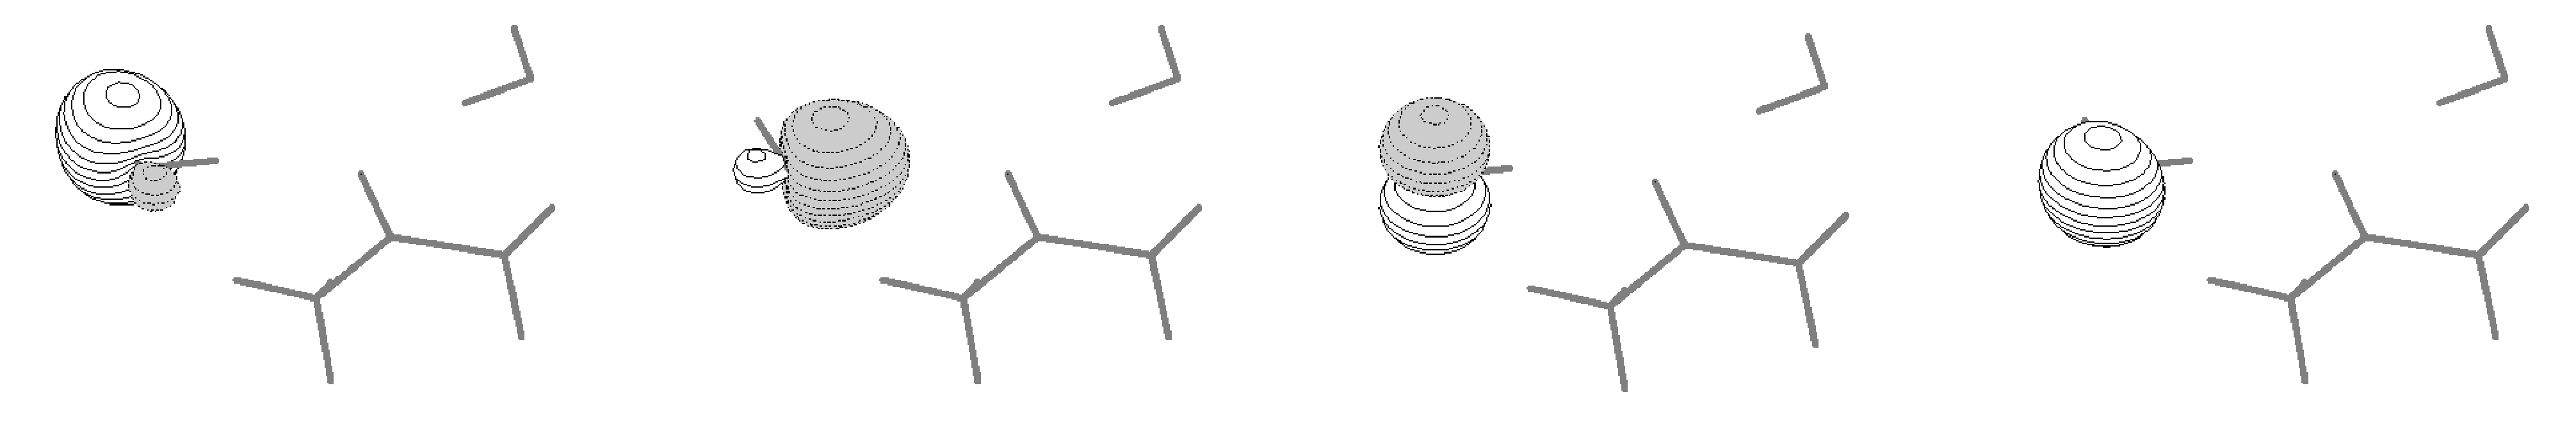
\includegraphics[width=11cm]{03_nevpt/images/h2o-loc.eps}
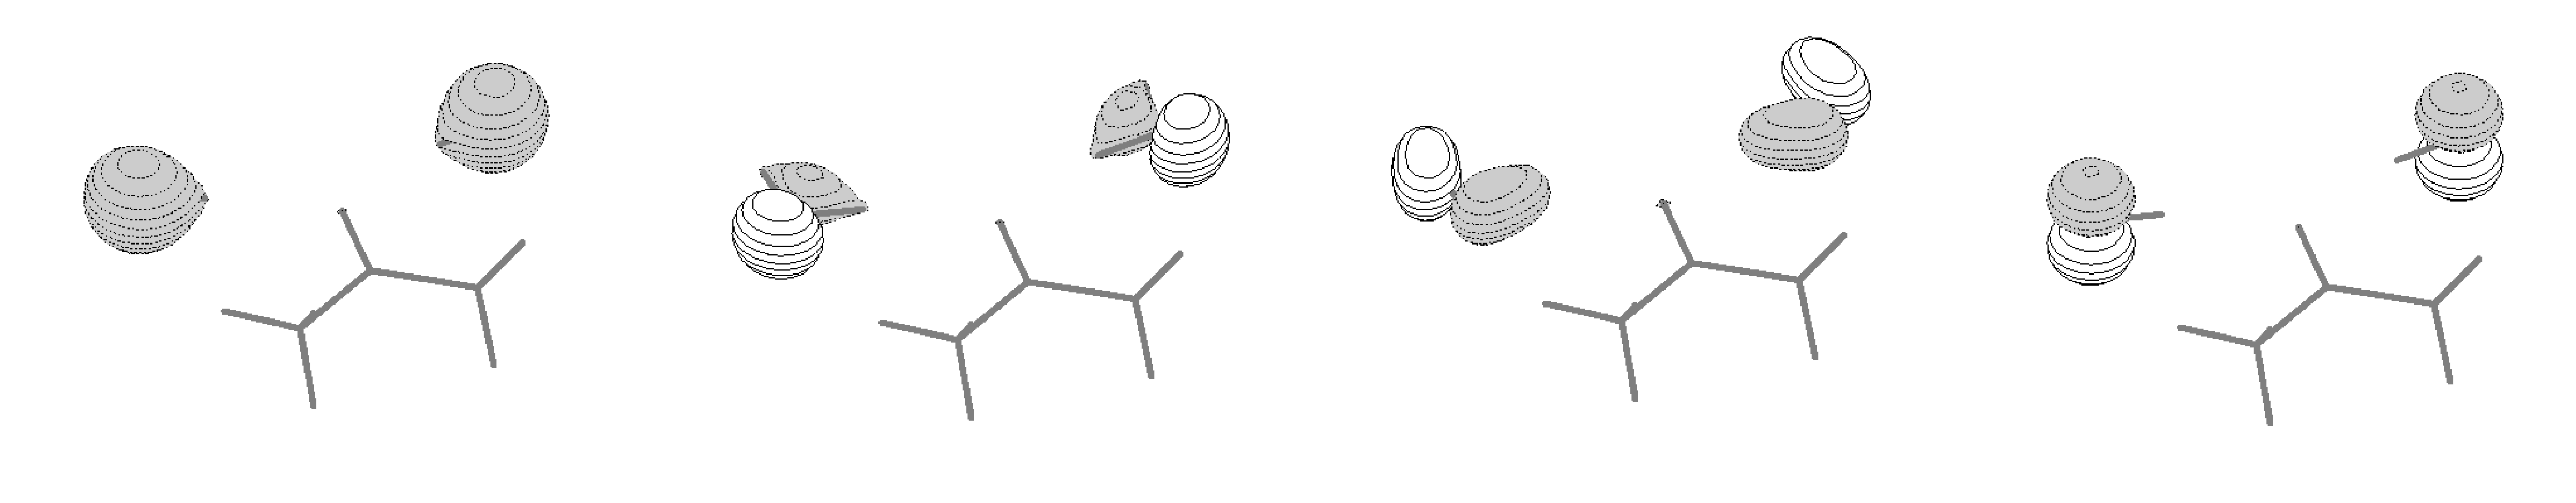
\includegraphics[width=11cm]{03_nevpt/images/h2o-deloc.eps}
\end{center}
\caption{\footnotesize A sample plot of non canonical localized orbitals
(upper part of the figure) and canonical delocalized orbitals (lower part)
for water orbitals. }
\label{fig:h2o-orb}
\end{figure}
\end{center}


Evaluating the energy difference provides consistency of the results.  For
the reported test, no high difference in the relative energies can be found,
as can be seen in Tab. \ref{tbl:noncanonical_energy}.

\begin{center}
\begin{threeparttable}
\begin{tabular*}{0.80\textwidth}{l@{\hspace*{27mm}}cccc}
\hline
        &  Ground   &  Excited    & Diff. \\
\hline
CASSCF   & -343.573883 & -343.411249 & 4.42 \\
SS-NEVPT & -343.766673 & -343.602997 & 4.45 \\
NC-NEVPT & -343.772194 & -343.609153 & 4.43 \\
\hline                                 
\end{tabular*}
\caption{\footnotesize Absolute energies and their differences for the
acetone+2 H$_2$O system. From the comparison of the relative excitation
energies, no high differencies between the methods can be found in the
analyzed system.
}
\label{tbl:noncanonical_energy}
\end{threeparttable}
\end{center}


This must be further investigated, given the small basis set used. However,
the target of this investigation was to demonstrate the consistency of the
NC-NEVPT results.




\cleardoublepage
\pagestyle{empty}
\begin{center}
{\Huge \textbf Resum\'e chapitre \ref{chp:grid} \\ Integration de reseau}
\end{center}

La puissance computationnelle et l'espace disque ont connu une incroyable
augmentation depuis quelques ans. La vitesse d'interconnexion r\'eseau est
aussi augment\'ee, et cet incr\'ement ouvre des nouvelles possibilit\'es pour obtenir
puissance computationnelle et espace disque utilisant plusieurs ordinateurs
peu employ\'e, \`a cr\'eer une m\'eta-plateforme commune: le r\'eseau \`a grid.
Avec une r\'eseau \`a grid, il est possible obtenir
\begin{itemize}
\item ressources d'infrastructure physique, comme espace disque, temp de
calcul, espace RAM, agr\'egation et archiviation des donn\'ees, utilisation
condivise d'instrumentation.
\item ressources logiques, comme exp\'erimentation, analyse des donn\'ees,
mod\'elisation et simulation.
\item ressources humaines, comme condivision des comp\'etences et communication
\end{itemize}

Le r\'esultat est un syst\`eme h\'et\'erog\`ene distribu\'e, qui donne une structure
virtuelle \`a l'utilisateur. L'interaction avec les services est
standardis\'ee et uniforme, sans probl\`emes d'architecture de CPU ou de
localisation g\'eographique de l'utilisateur.

Le r\'eseau \`a grid le plus connu est probablement le web. Le WWW est un
r\'eseau pour le stockage des donn\'ees. Ces donn\'ees sont consult\'ees
avec une interface standard, le navigateur web, avec une protocole \`a bas
niveau, l'HTTP. Cette abstraction est suffisante pour lire et \'ecrire
fichiers ou ex\'ecuter un script.

En ce moment, trois types d'applications peuvent \^etre d\'ecrit pour le
r\'eseau
\begin{itemize}
\item \textit{Applications \`a communication r\'eduite}: o\`u le probl\`eme est
d\'ecompos\'e en morceaux presque ind\'ependant, et le calcul est
effectu\'e sur chaque morceau. Seti@Home\cite{seti-site} ou le calculs
m\'et\'eorologiques sont des exemples.
\item \textit{Applications \`a pas}: o\`u la proc\'edure est d\'ecompos\'e en pas
s\'equentiels, chacun effectu\'e dans l'environnement de le reseau \`a grid.
Cette approche est utilis\'ee pour partager l'acc\'es \`a des instruments et
l'\'elaboration des r\'esultats, la distribution du co\^ut d'administration
et l'acces aux logiciels locaux.
\item \textit{Acc\'es \`a ressources}: pour partager ressources comme
bas des donn\'ees, instrumentation, espace de stockage.
\end{itemize}

Pour les processus de chimie quantique, de l'exp\'erience a \'et\'e faite avec la
parall\'elisation des algorithmes avec PVM et MPI, mais les \'evaluations
\textit{ab initio} sont principalement s\'equentiels: normalement, on a l'\'evaluation des
integrales, l'optimisation d'un fonction d'onde, et l'application d'autres
techniques. L'architecture de r\'ef\'erence est donc l'Applications \`a pas.

Le reseau Metachem est un type de reseau d\'evelopp\'e dans le cadre d'une action
COST de la communaut\'e europ\'eenne. L'objectif est l'int\'egration
de logiciels de chimie quantique mis \`a disposition par plusieurs
laboratoires europ\'eens.

Pendant ce travail de th\`ese, deux probl\`emes pour l'int\'egration ont \'et\'e
\'etudi\'e et r\'esolus. 
Le premier probl\`eme est le d\'eveloppement d'un format de fichier commun
pour \'echanger information binaire. 
Le formats de fichier dej\`a d\'evelopp\'es ont \'et\'e analis\'es, et 
leur d\'efects pour l'ex\'ecution en grid ont \'et\'e evalu\'es. Une reseau
\`a grid n\'ecessite de consid\'erations additionnelles: le format ne doit
pas \^etre platform-dependent, parce que le reseau peut \^etre construit
avec ordinateurs ayant des architectures diff\'erentes.  Le format id\'eal
pour ce travail est HDF5, mais malheureusement ce format est complexe \`a
utiliser. Autres consid\'erations sont la simplicit\'e d'utilise de la
biblioth\`eque d'acces, exactitude des messages d'erreur pendant l'acces et
extensibilit\'e du format.

La recherche effectu\'ee a conduit au d\'eveloppement d'un mod\`ele des
donn\'ees qui a \'et\'e impl\'ement\'e dans la biblioth\`eque Q5Cost. Cette
biblioth\`eque donner l'acces \`a des entit\'ees chimiques et simplifie
l'utilisation \`a des programmateurs avec une exp\'erience chimique.

Q5Cost a \'et\'e utilis\'ee pour l'integration des diff\'erents logiciels,
et ouvre des nouvelles possibilit\'es pour le partage d'information
quantistique et l'integration des m\'ethodes \textit{ab initio}.
La biblioth\`eque a aussi une testsuite pour contr\^oler l'interface et
chercher les probl\`emes dans l'implementation. 
Le r\'esultat est une biblioth\`eque tr\`es solide et extensible.

Le probl\`emes principaux qui restent \`a resoudre dans Q5Cost sont: le
stockage des integrals n'est pas encore efficient en terms d'espace
occup\'e, et l'implementation du mod\`ele des donn\'ees n'est pas complete,
mais l'impl\'ementation courante est suffisante pour le premiers
d\'eveloppements et implementations.

Le deuxi\`eme probl\`eme est le management de la s\'equence d'op\'erations
\`a effectuer et la conversion de ces instructions dans un format local pour
chaque logiciel. Cette conversion doit \^etre effectu\'ee par un logiciel wrapper
\`a l'entr\'ee et \`a la sortie, et donc est fortement li\'ee au logiciel
impliqu\'e.
La s\'equence des op\'erations sera probablement d\'ecrite avec le format
de fichier XML, et donc une biblioth\`eque de lecture et \'ecriture de ce
format avec le langage Fortran, F90xml, a \'et\'e d\'evelopp\'ee. Cette
biblioth\`eque interface libgdome2 (biblioth\`eque pour le langage C) avec
Fortran. 

Des exp\'eriences pr\'eliminaires de communication des donn\'ees ont \'et\'e
effectu\'ees, et les r\'esultats sont tr\`es encourageants.


\cleardoublepage
\pagestyle{fancy}
\chapter{Grid integration}
\label{chp:grid}
%\pagenumbering{arabic}

Computational power is cheap. Storage is also cheap and networking as well.
A well known empirical law for the increase of processing power is the Moore's law
\cite{moore-law}, which dictates the doubling of computational speed every
18 months. Similar laws have been envised for networking (doubling every 9
months) and storage capacity (doubling every 12 months). For scientific
needs, computational power and storage often are the limiting factors
for new developments and insights. 

The dramatic increase of networking performances opens new possibilities to
obtain computational power and storage from unused or underutilized
resources.  This deploys the fundation of a new paradigm for distributed
computing: grid metasystems.  Using grids, it is possible to pool
\begin{itemize}
\item \textit{Fabric resources}, like disk space, computational power, RAM storage,
data aggregation and archiviation, instruments
\item \textit{Logical resources}, like experimentation, data analysis, modeling,
simulation
\item \textit{Human resources}, like competence sharing, administrative burden,
communication.
\end{itemize}
The result is a distributed, heterogeneous metasystem, which provides a
virtual structure to the end user.  Interaction with services is
standardized and uniform, regardless of differences like CPU architecture
or geographical location. In this panorama, a grid provides
virtually infinite resources ready to use to produce a better science.

The most famous example of a grid is probably the Web. The well-known WWW is
a very simple storage grid where documents and informations are
geographically distributed. Users can access these informations through a
well-known interface (a web browser) which makes use of a low-level
uniform protocol (HTTP\cite{http-site}) in order to access resources.
The abstraction provided by the Apache webserver\cite{apache-site}
translates the HTTP requests into fabric level access, like reading or
writing a given file, or running a script.

Consortiums like IETF\cite{ietf-site}, W3C\cite{w3c-site} and
OASIS\cite{oasis-site} ratified standards in order to define
guidelines from low-level issues to high-level protocols and interactions:
TCP/IP\cite{tcp-site,ip-site}, HTTP, XML\cite{xml-site},
SOAP\cite{soap-site}, WSDL \cite{wsdl-site}, UDDI \cite{uddi-site}, RDF
\cite{rdf-site}, WSFL \cite{wsfl-site} are some examples of these standards.
Toolkits, frameworks and utilities have been developed, both commercial and
opensource to exploit the grid paradigm: Legion \cite{legion-site}, Globus
\cite{globus-site,ogsa-site}, and Unicore \cite{unicore-site} are some examples.

At the moment, a restricted set of grid applications can be devised:
\begin{itemize}
\item \textit{Low communication applications}: also known as ``embarassingly
parallel'' applications. For these applications, the problem is decomposed in
small almost independent pieces (usually called \textit{Working Units}),
and the computation is carried over each working unit. This category is
well represented by Seti@Home\cite{seti-site} or weather analysis
\item \textit{Staged applications}: the procedure is decomposed in
serialized steps, each one performed on a given site on the grid. This
approach is useful to manage human factors, like competence sharing and
administrative burden, license problems, use of private code, security
reasons
\item \textit{Resource access}: a resource from a service provider is made
accessible by request. Classic examples could be databases, instruments,
storage farms.
\end{itemize}

For quantum chemical processes some experience has been made, mainly with
parallelization of various algorithms (using PVM \cite{pvm-site}, MPI \cite{mpi-site} or OpenMP
\cite{openmp-site}). However, quantum chemistry evaluations are mainly
serialized in nature: for \textit{ab initio} calculations, a step involving
the evaluation of integrals is followed by other treatments, which in turn
provide information for others and so on.  This calls for a ``Staged
application'' architecture. This architecture is also enforced by
administrative issues, competence sharing and license problems, and finally
a current intrinsic complexity in the creation of multiplatform codes.

\section{Metachem grid}

The Metachem grid is a project for producing ``a meta-laboratory for code
integration in \textit{ab initio} methods''. The project, still in
development, has been carried on under the D23 COST action \cite{cost-site},
with the objective to develop a common grid infrastructure where
computational chemists can access several \textit{ab initio} codes produced
by different laboratories through a simple and user-friendly interface.

Most of the interested parties developed quantum chemistry codes for
{Post-SCF} evaluations, mainly for internal research. These techniques can be
integrated in a common infrastructure, but with the requisite to leave each code
on the platform it was originally designed for, under the responsibility of
its owner for maintenance and production. This will distribute the
administrative burden and avoid binary code duplication.

Finally, a set of standard quantum chemistry codes (\texttt{MOLCAS},
\texttt{COLUMBUS} or \texttt{DALTON}) must be integrated into the grid to
provide commonly used entities, like integrals, overlap, CASSCF orbitals and
wavefunctions, and so on.

Various considerations, ranging from technical factors to license
restrictions prevent direct changes to existing codes. A more conservative
strategy has been considered, at least in the initial deployment of the
project (see Fig.~\ref{fig:wrapper-scheme}): input and output wrappers
convert files and workflow logic between the local environment of a given
program and the shared grid environment, and viceversa. Input wrappers
convert information provided by the grid to low-level input such as Fortran
namelists and proprietary binary files. Output wrappers parse the products
of the program and create the standard information which will return to the
grid.

\begin{center}
\begin{figure}[ht]
\begin{center}
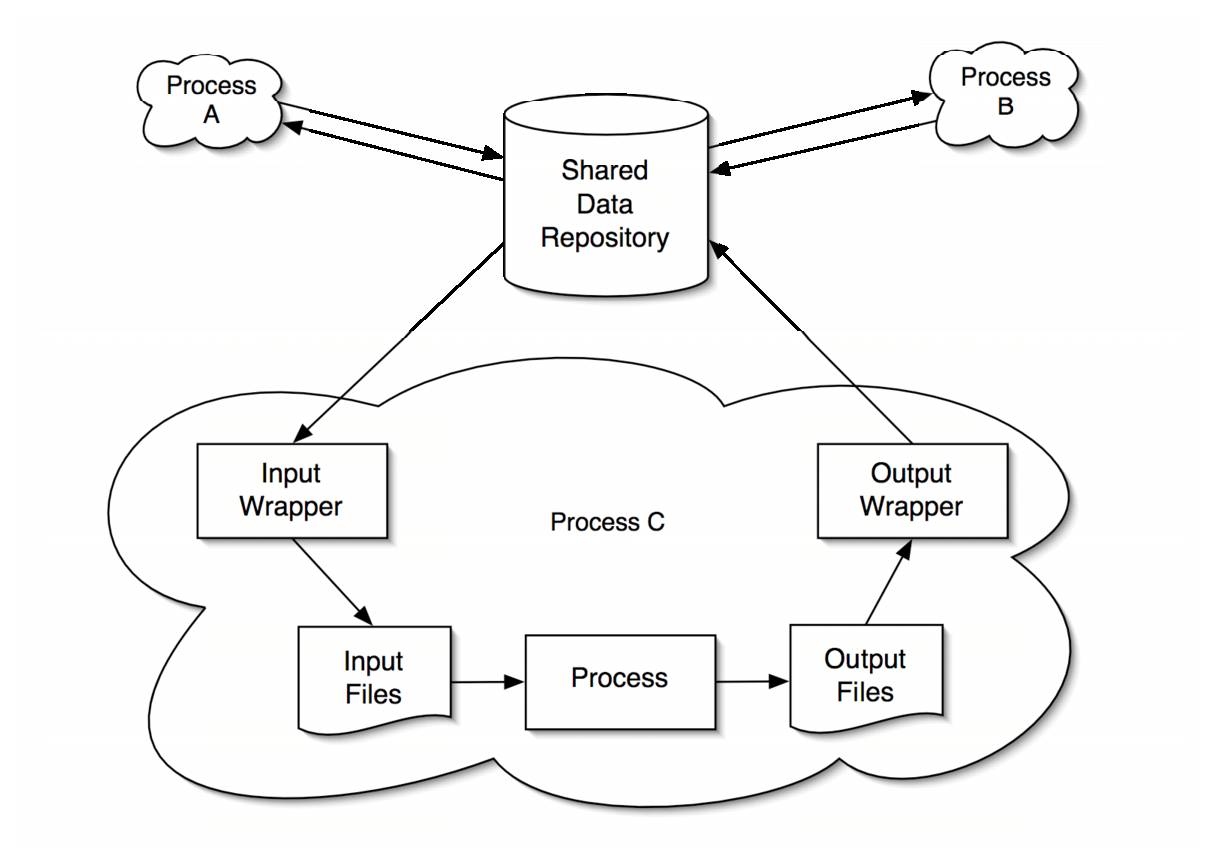
\includegraphics[width=10cm,keepaspectratio]{04_grid/images/wrapper-scheme-gimped.eps}
\end{center}
\caption{\footnotesize A scheme for the data handling inside a single
calculation environment. Data are made available by the data repository,
adapted to the local input environment of the process. The result is
converted back to the standard format and returned to the repository.}
\label{fig:wrapper-scheme}
\end{figure}
\end{center}


This strategy imposes the development and maintenance of the wrappers by
the interested parties. They are supposed to track the changes of their own
codes and adapt the wrappers accordingly. For historical reasons,
the reference language for the development of these wrappers is Fortran. 

The shared environment must also agree on a common file format.  Due to the
nature of the project, this common file format must be platform independent,
code independent, and easy to debug. Two different kinds of information have
been identified in quantum chemistry calculations:
\begin{itemize}
\item \textit{small data}, mainly ASCII encoded, like atom labels, geometry,
symmetry, basis sets, but also workflow specific information
\item \textit{large data}, normally binary encoded, like integrals and expansion coefficients
\end{itemize}

For the first kind of data, many initiatives are active nowadays. The more
extensive is the work of Murray-Rust et al.\cite{jcics-39-928-1999,
jcics-41-1113-2001,jcics-41-1124-2001,cc-1471-2000,njc-618-2001} with the
development of CML (Chemistry Markup Language) under the eScience project in
UK. The choice of XML allows both human readability and machine parsing.

Unfortunately, CML does not provide direct support for quantum chemical
entities.  After a brief analysis of the problem, an experimental
\textit{XML-schema} for quantum chemistry entities, QCML (Quantum Chemistry
Markup Language) has been deployed. The parsing of this information in
Fortran is possible through a library, named F77/F90xml, specifically
developed for the project.

For the second kind of data (large binary data) XML is not a good
technology, mainly due to its verbosity. For several reasons,
HDF5\cite{hdf5-site} is considered the best technology for large binary
data.

The next step, to be done in the future, is the definition and setup of
user defined workflows based on heterogeneous codes, located on different
platforms, communicating through the common formats. The actual technology
has yet to be chosen, but the choice seems to be oriented towards
UNICORE\cite{streit-tbp-2005,erwin-unicore,unicore-site}, together with a
common language for describing both workflow and intrinsic differences
between work paths. 

The final infrastructure is expected to satisfy both grid requirements
(fault tolerance, reliability) and human interface requirements (access via
web interface or specialized clients). An access point to grid services will be provided by
the CINECA supercomputing center. Its role is to coordinate the federated
system, where each node provides one or more services to the grid.


\section{Q5Cost library}

In the deployment of a common suite of codes, a standard file format is
necessary.  A first attempt in file standardization has been made in
Toulouse with the COST format. This format has been also implemented in most
of the Ferrara suite.

The format is made of four files, each one with a different extension:
\begin{itemize}
\item \texttt{.Mono}, a binary file containing the atomic basis set overlap and the one-electron
integrals on the molecular orbital basis set
\item \texttt{.ijcl}, a binary file containing the two-electron integrals
on the molecular orbital basis set
\item \texttt{.Info}, a cleartext file containing namelists describing various
metainformation, like the number of active orbitals, the nuclear
repulsion energy, the geometry and so on
\item a file called \texttt{INPORB}, containing the molecular orbitals. The format is
the same provided by the \molcas program, enriched with additional
information needed by the Toulouse suite of programs.
\end{itemize}

The COST files are written using the standard sequential access provided by
\texttt{READ} and \texttt{WRITE} statements in Fortran. No
{intention-revealing} interfaces are provided for accessing the data. This
implementation, although simple to manage, is limited in a lot of points:

\begin{itemize}
\item the standard sequential access provided by Fortran imposes to agree
on data size, data ordering, and chunking. It does not allow random access,
making difficult to update already written information, or to posticipate
the writing operation of some entity. It complicates reorganization
or expansion of the stored information set
\item files are not platform independent. A file written on an Intel
x86 machine is unreadable by an IBM SP4 supercomputer, and viceversa. This
limits the output sharing
\item it is difficult to access the stored information in a clear
representation. This is a major issue when debugging computational chemistry
codes. At the moment the access is through ad-hoc visualizers or hexadecimal
editors
\item the file is difficult to split, merge, compare, or describe with
metainformation
\item the API for accessing the file format is limited in features,
allowing no basic consistency checks or a clean interface. Documentation 
is written as code comments. This makes difficult to direcly access the
information.
\end{itemize}

Q5Cost is a library devoted to solve these problems. Based on the
{platform-independent} file format HDF5, Q5Cost allows the user to produce binary
files through a well documented interface. The library also takes care of
providing useful information during debug, explicitly stating inconsistent
data or wrong usage of the routines.

\subsection*{HDF5 file format}

As defined on the website\cite{hdf5-site}, ``HDF5 is a general purpose library and file
format for storing scientific data''. HDF5 targets the data management needs
of scientists and engineers working in high performance, data intensive
computing environments. This is achieved by providing an efficient library and
file format, specifically tuned to read and write binary data efficiently.

A HDF5 file appears to the user as a single file containing a structured
graph of entities. This structure is conceptually very similar to a UNIX
filesystem, and is defined by means of three entities: \textit{Groups},
similar to directories, \textit{Datasets}, similar to files
and \textit{Attributes}, similar to metainformation such as permissions and
owner.  Data are stored into Datasets and Attributes, and can be organized
with Groups. The HDF5 library provides an interface to handle these
entities.

The most striking feature of HDF5 is the platform independence of the files.
A file written on a 32 bit Little Endian architecture (like, for example, an
Intel x86 machine) can be transferred and read transparently on a 64 bit Big
Endian machine (like, for example, the IBM SP4) or a 64 bit Little Endian
machine (like an IA64 machine). This is of critical importance
in grid environments, where heterogeneity is the rule, rather than the
exception.

Another important feature of HDF5 is the suite of utilities, which allows the
user to find differences between two HDF5 files, obtain a textual dump of
Groups, Datasets and Attributes layout (resembling the ``ls'' program in
UNIX environment) or a more detailed view presenting also the numerical
data.  This simplifies the access to this information, which is critical
in the debug phase.

The HDF5 library is made of a directly accessible C layer. Alternative APIs
are available for C++, Fortran 90, and Java. The library is actively
developed, is free and released as open source software.

\subsection*{Q5Cost file format and library} 

The Q5Cost library is implemented on top of the HDF5 library.  It provides
read and write access to HDF5 files with a specifically designed high-level
interface for quantum chemistry developers. 

The rationale is to provide a Fortran interface based on well known chemical
entities, rather
than groups or datasets like in the HDF5 interface. HDF5 takes care of
low-level management of the file, and Q5Cost provides the high-level
API to store and retrieve chemical entities.

An extensible data model has been rationalized thanks to the knowledge
obtained by the involved researchers. Some firm points have been
discovered.

The first point is that many different types of simple and small data
must be handled. Some examples are nuclear energy, molecular orbital labels,
molecular symmetry and so on. We will refer to these data as
\textit{metadata}, in order to distinguish them from the real large
information on the chemical system, the integral values.

Metadata represents well-known chemical entities and belong to three
generic data classes: \textit{Scalars}, \textit{Vectors} and
\textit{Matrixes}. For example, the nuclear repulsion energy is a floating
point scalar, molecular orbitals can be represented as a (N,M) floating point matrix, the
associated orbital energies is a floating point vector, the molecular
orbital labels is a vector of strings and so on. The library should provide
an interface for accessing these data, both as generic or specialized
entities.

A second point is the fact that in quantum chemistry large sparse
matrixes with an arbitrary number of indexes (rank-$n$ arrays) are very
common data structures. These data usually scale aggressively with the
system size, and they are normally accessed with a chunked sequential approach.
This is the case of entities like two-electron integrals, or atomic
orbitals overlap, but also much other more application-specific
information, like the four-particles density matrix.

The sparse nature of these matrixes encourages to store only non-zero
elements, each one associated to $n$ indexes in the case of a rank-$n$
array. This representation of the data, although not always efficient in
term of space occupation, is well known by the interested parties, easy to
debug and already integrated in the current codebase both for memory
representation and file storage. The library structure allows 
future expansions of the low-level storage format, in order to reduce the
storage needs, but in the first development phase this issue has not
been investigated, and the current format is useful for the direct debug of
the file.

These large data arrays share common features:
\begin{itemize}
\item they usually are integrals, whose evaluation involves one
operator and a given number of functions. These functions are
referred by the indexes of the matrix. For example, two-electron integrals
on the molecular orbital basis are stored as a rank-4 array with indexes
referring to the molecular orbitals. In the case of atomic basis set overlap
integrals, the indexes refer to the atomic basis set
\item the rank of the array depends on the physical meaning of the
integrals. Atomic basis set overlap is described by two indexes, and can be
stored as a rank-2 array. Two-electron integrals have four indexes imposing a
rank-4 array and the four-particles density matrix has eight indexes,
requiring a rank-8 array
\item additional information is needed to describe the involved operator
(for example its symmetry) and the entities the indexes refer to.
\end{itemize}

All this information can be classified under a generalized \textit{Property}
concept, which is described by the matrix rank and the definition of the
involved operator and functions. Integrals are stored by means of a
dedicated abstraction, named \textit{CompactMatrix}, enriched with
metadata to define the Property, like its name, rank, symmetry and
real/complex nature.

Some properties are well-known chemical entities, and chemists are
used to refer to them by name. A specific library access has been provided
to handle these entities, easing the need to specify well-known information
about them.

A further step is to recognize containment relationships and simple
consistency patterns between the involved entities. A graphical
representation can be seen in Fig. \ref{fig:q5cost-schema}.

\begin{center}
\begin{figure}[ht]
\begin{center}
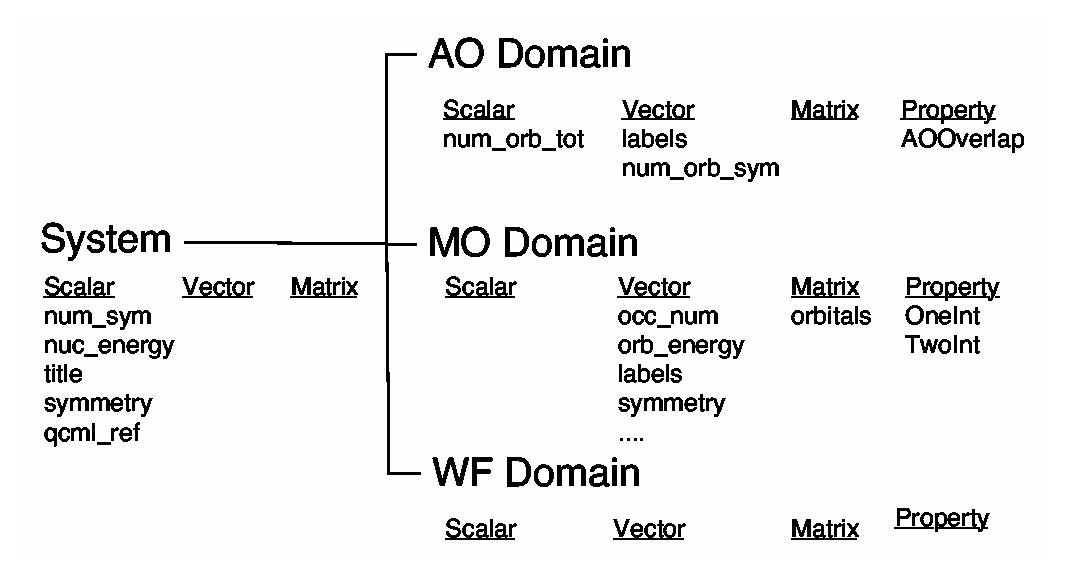
\includegraphics[width=10cm,keepaspectratio]{04_grid/images/q5cost-schema-gimped.eps}
\end{center}
\caption{\footnotesize A graphical representation of the containment
relationship between the System and the Domains. Specific metainformation is also
presented, classified under the appropriate environment.
}
\label{fig:q5cost-schema}
\end{figure}
\end{center}


The first high-level logical container is the \textit{System} object. This
object represent a molecular system as described by its structural
informations, such as symmetry and atomic coordinates, and also contains all
the metadata that are invariant at this level, like for example nuclear
repulsion energy, or a title. Multiple Systems make possible to handle
different molecular geometries.

A System can contain several \textit{Domains}. The role of a Domain is to
group together Properties whose indexes conceptually refer to the
same entity. Three Domains have been recognized as fundamental: \textit{AO}
for Atomic Orbital, \textit{MO} for Molecular Orbitals and \textit{WF} for
Wavefunction.  Each Domain can contain an arbitrary number of Properties, and
additional metadata represented as specialization of Scalar, Vector and Matrix
entities.

The AO Domain holds Properties whose indexes refer to the atomic basis set
funtions: overlap, one-electron and two-electron integrals on the atomic
basis set are some examples, in addition to the generic Property. The
associated metadata hold information about the atomic orbitals, like their
number, labels and symmetry.

The MO Domain holds Properties referring to molecular orbitals:
one-electron and two-electron integrals on the MO basis set are examples, in
addition to the generic Property. The descriptive metadata refer to the
molecular orbitals, their number, labels and symmetry, the AO
basis they were derived from, orbital energies, classification and
occupation numbers.

The WF Domain holds Properties referring to the electronic states. At the
moment a complete definition of this Domain is not available and not
subjected to major research and development, given its non-critical nature
for the first deployment of the library.

Each Domain can be defined under different occurrences, by means of a textual
identifier (\textit{tag}) chosen by the user, with a default value if no tag is
provided. The aim is to provide storage of multiple entries for each Domain,
like in case of multiple molecular orbitals in the MO Domain, or multiple
basis sets in the AO Domain.

\subsection*{Library structure}

The library is written in Fortran 95 and is made of different modules, each
one providing different facilities. The most important modules are

\begin{itemize}
\item \textit{Q5Cost}: defines the high-level API, providing
subroutines designed to be accessible from the final programmers of the
laboratories involved in the project
\item \textit{Q5Core}: provides a wrapping facility for HDF5 routines, in order to
perform additional useful services like reference counting and debugging.
Also provides simplified routines to perform frequently used low-level
tasks
\item \textit{Q5Error}: provides facilities for high-level debugging of the
library and client codes. This module implements a ring buffer for error
messages, different logging levels, generic reference counting for catching
leaks of HDF5 references, and a subroutine call stack trace.
\end{itemize}

Subroutines for each module have been namespaced with an appropriate prefix,
and names have been chosen to provide an explicit and {intention-revealing}
interface to the entities described in the previous section.  

Although Fortran 95 does not allow object oriented (OO) programming, some OO
concepts have been used in the development of the library, keeping into
account the procedural programming background of the final developers. The
state is preserved into the HDF5 file, and subroutines refer to the file
directly through the HDF5 identifier, a more easy concept for Fortran
programmers used to unit descriptors.

\subsubsection*{The Q5Cost module}

This module is the main reference for the final users. It provides
subroutines to read and write HDF5 files in the Q5Cost format with a high-level
abstraction. The users can deal with high-level concepts without worrying
about low-level implementation details. If a finer access is needed to the
underlying HDF5 file, the Q5Core module provides this access in a simpler
way with respect to raw HDF5 routines.

The Q5Cost module is made up of routines belonging to the following
classes:
\begin{itemize}
\item \textit{File}: create, open, close the file and write/read root
metainformation, like creation time, access time and file version
\item \textit{System}: create or check the existence of the System and set/get
its metainformation
\item \textit{AO}: create or check the existence of the AO Domain and set/get its
metainformation
\item \textit{AOOverlap}: create, read and write data for the atomic basis set
overlap Property
\item \textit{MO}: create or check the existence of the MO Domain and set/get its
metainformation
\item \textit{MOOneInt}: create, read and write data for the one-electron
integrals in molecular orbitals basis
\item \textit{MOTwoInt}: create, read and write data for the two-electron
integrals in molecular orbitals basis
\item \textit{WF}: create or check the existence of the WF Domain and set/get its
metainformation. Still experimental and mostly unimplemented.
\end{itemize}

Additional routines are provided for generic access to the Property
class, allowing to manage generic property data. Subroutines for
AOOverlap, MOOneInt and MOTwoInt delegate calls to these Property routines,
automatically passing well-known parameters about the involved property.

Q5Cost module routines provide a context-based access to chemical
entities. This access is transformed into a path-based access, creating
an appropriate layout for HDF5 groups, datasets and attributes, and
writing the user-provided data on the file. Some data are automatically
written by the library, like the creation or access time and the
Q5Cost library version. 

One important aspect of this format is that the user is not forced to
produce information for all quantities. The user can store only those
quantities that are actually available.  Constraint checks are however
mandatory in order to assure basic file consistency. For example, no MO
Domain can be created if a System and an AO Domain have not been provided,
in order to guarantee the presence of fundamental data, like the number of
symmetry species and the number of basis functions for each symmetry
species.

\subsubsection*{The Q5Core module}

The Q5Core module is a low-level module designed to provide wrapping
facilities between the Q5Cost library and the HDF5 library. At the moment it
is focused at providing additional debug information, reference counting
for HDF5 objects, additional low-level API to simplify common tasks.

This module also provides path-based creation of Scalar, Vector and
Matrix entities (in contrast with the context-based approach of the Q5Cost
module, which focuses on chemical concepts rather than HDF5 paths) and also
routines to ease handling of the Property index/value data, relative to the
CompactMatrix class. Most of the Property routines accessing index/value
data delegate to CompactMatrix subroutines. 

Q5Core module could also be useful to guarantee transparency toward a
low-level format migration from HDF5 to other storage formats. This could
allow the Q5Cost module to remain unchanged and unaware of the final
low-level format, but in the current deployment this was not a priority.
Final users are not expected to access Q5Core module routines, except for
highly experimental tasks.

\subsubsection*{The Q5Error module}

The Q5Error module provides subroutines to monitor the behavior of the
library and the client code. A ring buffer is provided to keep track of
error messages generated by the library. A verbosity level can be set from
totally silent to highly verbose, where each subroutine call and return are
reported into the buffer. Also, a stack for backtracing has been implemented
to keep track of the call tree. The tree is printed out when an error occurs
and error reporting is requested. 

Different specific error codes have been devised to report anomalous
behavior to the client code or to the library itself. Error codes are
defined as numeric parameters and report situations ranging from invalid
parameters to non-existence of some information into the file. The presence
of an error condition is reported to the client code through the last
parameter of each subroutine.

\subsubsection*{Additional details: testsuite and documentation}

A dedicated module for testsuite deployment and a set of tests have been
implemented to stress the library through a high number of well-known
critical situations, evaluating the correctness of the response. At the
moment, more than 300 tests are implemented, covering the most common usage
patterns. Reference counting is checked to prevent leaks of HDF5
references. The testsuite provides an effective watchdog for debugging,
refactoring, and bugfixing.

Library documentation is embedded into the Fortran code as comments,
using a custom markup system.  A simple parser, written in the
Python\cite{python-site} programming language, extracts the documentation
producing HTML files.

\section{Q5Cost examples}

Various programs have been implemented using Q5Cost: \texttt{q5dump},
\texttt{cas2hdf}, \texttt{hdf2cost} and, of course, the testsuite presented
in the previous section.

\texttt{q5dump} is a program designed and implemented by Antonio Monari.
It allows access to the information inside a Q5Cost file in a clean and
explicit way. It resembles the \texttt{h5dump} utility from the HDF5
library, but \texttt{q5dump} presents information in chemical speech,
rather than low-level HDF5 concepts like groups and datasets.

A typical output of the program is reported

{\footnotesize
\begin{verbatim}
 ************************************
 *          Q5Costdump              *
 *                                  *
 *     a tool for analysis of       *
 *           Q5Cost files           *
 *                                  *
 ************************************
 
 Creation time 2005/03/30  15.28.05
 
 SYSTEM ATTRIBUTES
 Title: LiHs33                                                          
 Order of the symmetry group  4
 Nuclear Repulsion (Core Energy)  0.995024875621900007
 
 Groups present  2
 ao 1
 tag-default
 mo 1
 tag-default
 ------------------------------------------------------
 
 Properties of AO group <default>
 
 Number of Orbitals 33
 Orbital in Symm. Classes   17   7   7   2
 AO is empty
 ------------------------------------------------------
 
 Properties of MO group <default>
  AO REF: <default>
 
 Number of Orbitals 33
 Orbital in Symm. Classes   17   7   7   2
 
 dipolex is present
 dipolez is present
 oneint is present
 twoint is present
 orbitals is empty
 
 ------------------------------------------------------

\end{verbatim}
}
which can be compared against the output produced by \texttt{h5ls}
{\footnotesize
\begin{verbatim} 
/ao                      Group
/ao/tag-default          Group
/mo                      Group
/mo/tag-default          Group
/mo/tag-default/Property-dipolex Group
/mo/tag-default/Property-dipolex/CompactMatrix-data Group
/mo/tag-default/Property-dipolex/CompactMatrix-data/index Dataset {2, 171/Inf}
/mo/tag-default/Property-dipolex/CompactMatrix-data/value Dataset {171/Inf}
/mo/tag-default/Property-dipolez Group
/mo/tag-default/Property-dipolez/CompactMatrix-data Group
/mo/tag-default/Property-dipolez/CompactMatrix-data/index Dataset {2, 181/Inf}
/mo/tag-default/Property-dipolez/CompactMatrix-data/value Dataset {181/Inf}
/mo/tag-default/Property-oneint Group
/mo/tag-default/Property-oneint/CompactMatrix-data Group
/mo/tag-default/Property-oneint/CompactMatrix-data/index Dataset {2, 182/Inf}
/mo/tag-default/Property-oneint/CompactMatrix-data/value Dataset {182/Inf}
/mo/tag-default/Property-twoint Group
/mo/tag-default/Property-twoint/CompactMatrix-data Group
/mo/tag-default/Property-twoint/CompactMatrix-data/index Dataset {4, 39790/Inf}
/mo/tag-default/Property-twoint/CompactMatrix-data/value Dataset {39790/Inf}
/mo/tag-default/orbitals Dataset {0/Inf, 0/Inf}
\end{verbatim}
}

\texttt{cas2hdf} and \texttt{hdf2cost} are converter utilities, designed to
stress a first deployment of the library in a production environment.  In
Fig. \ref{fig:q5cost-final}, a representation of the final intended
procedure is depicted.
\begin{center}
\begin{figure}[ht]
\begin{center}
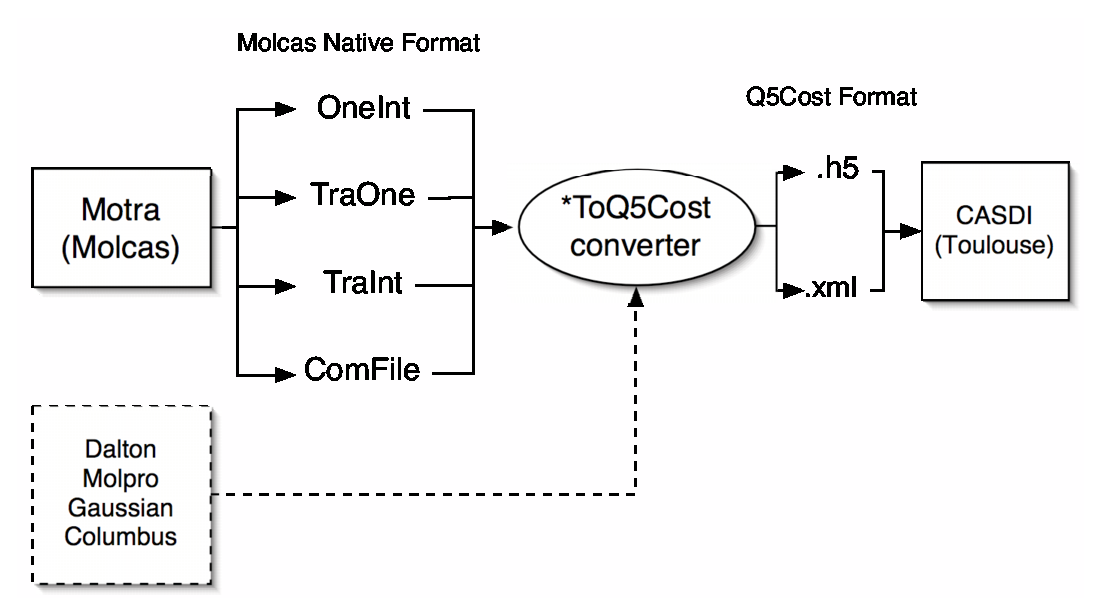
\includegraphics[width=10cm,keepaspectratio]{04_grid/images/q5cost-final-gimped.eps}
\end{center}
\caption{\footnotesize One of the possible final code layouts, involving
direct changes in the code. An integral producer, such as \texttt{MOLCAS}, provides
proprietary files. These files are fed to a converter, which creates the new
Q5Cost format. The program \texttt{CASDI} from Toulouse directly reads these
files. This infrastructure at the moment is not possible, because the
current \texttt{CASDI} implementation reads the old COST format.}
\label{fig:q5cost-final}
\end{figure}
\end{center}

Output integrals are produced by a commercial package, \molcas in the
example, but converters could be developed for other programs, like
\texttt{DALTON}, \texttt{COLUMBUS} and so on. These integrals are fed into a converter to
produce the Q5Cost file format, made of the HDF5 file and an XML (QCML) file
providing additional information. The Q5Cost format will be read by
CASDI, a program from the Toulouse chain of programs. This
approach assumes that \texttt{CASDI} is directly interfaced with the Q5Cost format. 

A more conservative way to handle this interface is represented in Fig.
\ref{fig:q5cost-intermediate}.
\begin{center}
\begin{figure}[ht]
\begin{center}
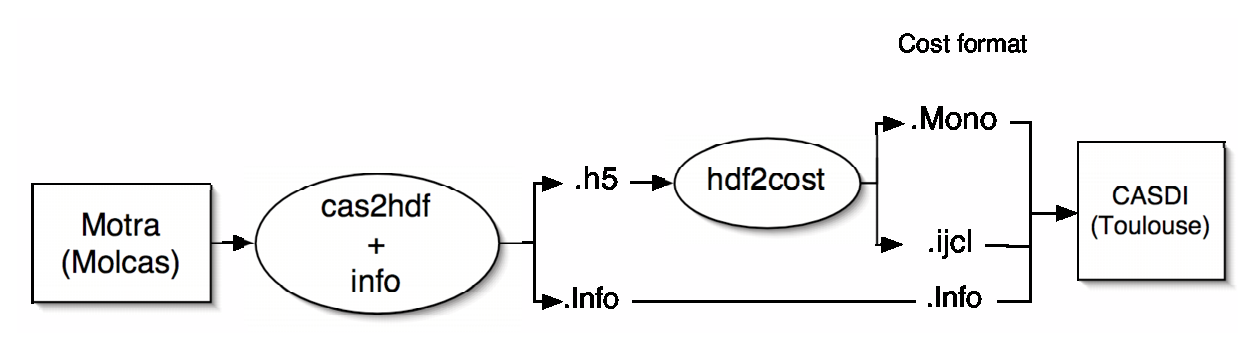
\includegraphics[width=10cm,keepaspectratio]{04_grid/images/q5cost-intermediate-gimped.eps}
\end{center}
\caption{\footnotesize A conservative solution. The \texttt{cas2hdf}
program produces the Q5Cost file, which is converted to the old COST format with
\texttt{hdf2cost}. The \texttt{.Info} file is used as a temporary
replacement of the XML file, and is provided by the \texttt{info}
program, directly interfaced with the \molcas suite. This solution does not
need changes in the CASDI code, and is therefore preferred in the initial
deployment. }
\label{fig:q5cost-intermediate}
\end{figure}
\end{center}

The \texttt{cas2hdf} program directly accesses the \molcas files, producing the
Q5Cost file. The \texttt{.Info} file is used as a temporary replacement of
the XML file, and it is provided by the \texttt{info} program.
The resulting Q5Cost file is read by \texttt{hdf2cost} and converted to the
old COST format, which can be directly read by CASDI.  This solution does
not need changes in the \texttt{CASDI} code, and is therefore preferred in the
initial deployment.

The deployment of these tools made possible to obtain a successful
interface between \molcas and \texttt{CASDI}. Some successful experiment has been also
performed with \texttt{DALTON}.

An experiment of direct integration has been performed with the
\texttt{Full-CI}\cite{cpl-252-437-1996,ijqc-48-287-2004} program developed
in the Professor Bendazzoli research group at Bologna University. The
\texttt{Full-CI} code is now able to read Q5Cost files, and can be
interfaced with both \molcas and \texttt{DALTON}.


\section{F77/F90xml library}

The Extensible Markup Language (XML) file format plays a central role in the
modern internet infrastructure. XML is derived by the more general format
Standard Generalized Markup Language (SGML), and is visually very similar to
HTML (the file format for web pages) although HTML itself is not a XML
document. 

The official definition provided by the W3 Consortium\cite{w3c-site} states
that the ``\textit{Extensible Markup Language (XML) is a simple, very flexible text
format derived from SGML (ISO 8879).  Originally designed to meet the
challenges of large-scale electronic publishing, XML is also playing an
increasingly important role in the exchange of a wide variety of data on the
Web and elsewhere}''.

The main advantages of this format are:
\begin{itemize}
\item internet standard, as accepted by the W3 Consortium
\item platform independent
\item clean and terse human readable textual format
\item very practical and extensible
\item can be checked for syntactical and semantical correctness
\item allows the description of data and their meaning
\item can be commented inline
\item already existent libraries for accessing the document
\end{itemize}

An example of an XML document is given below

\begin{verbatim}
<?xml version="1.0"?>
<book ISBN="0140390839">
 <!-- a comment -->
 <author>Mark Twain</author>
 <title>Tom Sawyer</title>
 <chapter>
  <title>First Chapter</title>
  This is the content of the first chapter.
 </chapter>
 <emptypage />
 <chapter>
  <title>Second Chapter</title>
  This is the content of the second chapter.
 </chapter>
</book>
\end{verbatim}

An XML document holds \textit{markup} and \textit{content}. The most common type of markup is
the \textit{Element}, delimited by angle brackets and normally present in pairs of
begin tag (for example ``\texttt{author}'') and end tag (the same tag name, but
prepended by a slash ``\texttt{/}'' symbol). These elements wrap content and other
markups in a nested parent/child relationship, defining a tree-like
structure. If an Element has no content, an alternative abbreviated syntax
can be used to represent the begin/end as a single tag. The
``\texttt{emptypage}'' Element is an example of such syntax.

Another kind of markup is the \textit{Attribute}. Attributes are name/value
pairs defined in the context of an Element. An example of this markup is the
``\texttt{ISBN}'' entry for the ``\texttt{book}'' Element.

Finally, a comment markup can be seen in the provided example.  Other kinds
of markups, such as processing instruction, entity references or CDATA
sections, will not be analyzed in this thesis.

Two constraints define the correctness of an XML document:
\begin{itemize}
\item \textit{well-formedness}
\item \textit{validity}
\end{itemize}

An XML document is well-formed if it complies with the XML specification.
Using square brakets instead of angular brakets is an example of non
well-formedness. Improper nesting of elements such as
\begin{verbatim}
 <author>Mark<Title>Twain</author>Tom Sawyer</title>
\end{verbatim}
is another example. XML Parsers must report an error when a non well-formed
document is provided.

Validity is related to well-formed documents that comply with a logical
meaning, related to the chosen data model. 
For example, the document
\begin{verbatim}
<?xml version="1.0"?>
<title>
 <book>
  Tom Sawyer
  <author ISBN="0140390839">
   <chapter>
    This is the content of the first chapter.
   </chapter>
  </author>
 </book>
</title>
\end{verbatim}
is a well-formed document, but has poor or no meaning in the analyzed data
model. Validity depends on the context and is defined by Document Type
Definitions, or XML-Schemas, which will not be detailed in this thesis. Pure
parsing cannot check for validity unless DTD or schemas are provided.

Accessing XML documents can be performed through two standardized interfaces:

\begin{itemize}
\item \textit{SAX}, Simple API for XML
\item \textit{DOM}, Document Object Model
\end{itemize}

SAX is an event-driven parser. While the document is read (from a file, or
from a network socket) the parser calls specific callback routines (handlers) to
process the current Element (start or stop markups), or Attribute, or
content (TextNode). Each handler is normally defined by the developer of the
client code, and expresses the contextual behavior related in finding a
certain Element, or TextNode.

SAX has some important advantages: first, parsing can be performed on a
partial document. This is very important if the document is very large, or
if the parsing must begin as soon as the first data are available. This
can produce a more pleasant experience of responsiveness to the user if, for
example, the document is downloaded from a slow network connection.

Second, the SAX parsing has a very small memory footprint. The document does
not need to be held in memory. Nodes can be parsed and discarded after the
event has been dispatched to the appropriate handler. This is very important
if the document is very large. 

SAX has also disadvantages: is a readonly parser (it can only read
documents, but cannot build and write an XML tree), is stateless, is purely
sequential, and finally is rather difficult to use. 

The other available parser is DOM. DOM is an interface to an
{Object Oriented} description of the XML document. The main advantage of DOM
is represented by the ability to handle the document in ways not provided by
SAX: DOM interface directly exposes the tree data abstraction in terms of
Nodes (\textit{flat interface}) or specialization of the Node concept, like Element,
Attribute, Document, TextNode, and so on (\textit{specialized interface}).
The document is parsed as a whole and a tree representation is built in
memory. This representation can be parsed, read and altered with a random
access approach, and finally written back to disk or to a network
connection. DOM interface is also simpler to use than SAX. 

The main drawback of DOM is the need to hold a complete representation of
the document in memory. For this reason, DOM parsing is generally not
applicable on partial or very large documents.

Two interface levels are available, and a third is almost ratified.
DOM Level 1 provides the basic handling of the tree. DOM Level 2 and 3
provide additional advanced features like namespacing and events. Only a
restricted set of Level 2 features are needed for the project.

\subsection*{XML and Fortran}

Calculations in scientific environments such as physics, chemistry,
astronomy and so on are still bound to the Fortran language.  Other
high-level languages such as C, C++, Java, Python are of difficult
deployment.  Techological problems (compatibility, library availability,
efficiency) human factors and historical reasons (learn new abstractions and
patterns, rewrite the legacy code) prevent a switch to other languages.

Of course, this is a strong limiting factor in keeping the pace with the
rapid evolution of network and computational resources. Using these new
technologies often requires dedicated middleware, specifically designed to
simplify access by wrapping low-level functionality with a high-level
interface. XML handling is an example of the reported situation: an XML
document is a plain text file, but its complex, extensible structure goes beyond
its pure textual nature. SAX and DOM parsers are high-level frontends to XML
document management, taking care of low-level issues and presenting a new
abstraction to the programmer.

The lack of a Fortran library to handle XML can be a problem when the
deployment of new standards is needed and the handling of these standards
must be performed by Fortran programmers, like in the case of the AbiGrid
project. Currently available libraries for XML access in Fortran are
``xml''\cite{xmllib-site} and {``xml-fortran''}\cite{xml-fortran-site}, 
not DOM compliant and written in pure Fortran, and ``xmlf90''
\cite{xmlf90-site} which supports SAX and DOM Level 1 and is written in the
F subset of Fortran.

Among the problems of these solutions are:

\begin{itemize}
\item non DOM Level 2 compliant (no namespaces support)
\item rather difficult to use and extend
\item read only
\item string handling is very rigid
\item bound to F90 compilers
\end{itemize}

The first five points are indeed critical. Deploying advanced features like
DOM or XPath (a standardized method to access Nodes using a syntax similar
to a filesystem path) is very difficult with a pure Fortran approach.
Fortran has limits in strings, file handling and object management.

The latter point is more controversial. Many commercial Fortran 90 compilers
exists. Some of them are available at no cost, but this policy could change
in the future. With the release of free Fortran 90 compilers like g95
\cite{g95-site} and gfortran \cite{gfortran-site}, the latter point is no
longer an issue, but was a prerequisite in the initial development of
F77/F90xml.

\section{F77/F90xml implementation}
% {{{
The F77/F90xml library \cite{f77f90xml-site} is a C library designed to
provide a Fortran interface to libgdome2 \cite{gdome2-site}, an opensource
library (also developed using C language) part of the GNOME
\cite{gnome-site} project. Most of the design is implemented to give access
to a DOM level 2 interface \cite{w3-dom-level-2-site}, with the exclusion of
events, which are not needed in the target environment. XPath support is
available, although no testing has been performed and therefore must be
considered experimental.

At the time of writing, F77/F90xml library depends on libgdome2-0.8.0,
glib-1.2.10 \cite{glib-site}, libxml2-2.5.11 \cite{libxml2-site}.  Building
of the library also depends on Python 2.3 \cite{python-site} or above.  The
library has been successfully compiled on Intel/AMD Linux platform, with gcc
and Intel Fortran Compiler, and IBM SP4 with the xlf compiler suite. It is
released under the terms of the LGPL \cite{lgpl-site}.

F77/F90xml has been designed with Fortran 77 backward compatibility in mind.
The library provides two interfaces: a Fortran 90/95 interface, similar to
DOM Level 2 in order to reduce the need for specialized documentation, and a
Fortran 77 interface, using specialized subroutines named
\textit{multiplexers}.

The Fortran 77 interface is particularly complex and error prone.  An
experimental preprocessor has been deployed to translate pseudo-F90 code
into F77 code, but Fortran 77 is very old and the choice for new code should
be Fortran 95. Support for this language was an initial request from the
interested parties, and provides full freedom even to those projects that
still work in a pure Fortran 77 environment for their maintenance. 

When the library development started, no stable and free Fortran 90/95
compiler existed, and most of the potentially interested parties had the
requisite to compile the code using the GNU F77 compiler.  This situation
changed with the release of g95 and gfortran, however the Fortran 77
interface is directly obtained from the implementation, simplifying rather
than making more difficult the development of the library.

In the following, we will refer to the Fortran 90 interface with the term
``F90xml'', and with ``F77xml'' to the specific Fortran 77 interface.
Finally, the term ``F77/F90xml'' refers to the library as a whole.
% }}}

\subsection*{The Fortran 90/95 interface}

The Fortran 90/95 interface provides a clean and simple access. All gdome2
functions are mapped to Fortran subroutines, collected together into a 
\texttt{MODULE}. A simple code example is provided 

{
\footnotesize
\begin{verbatim}
INTEGER :: first, last, elem, err

Comment <... get elem by some other call ...>

CALL f90xml_el_firstChild(first,elem,err)
CALL f90xml_el_lastChild(last,elem,err)
\end{verbatim}
}

which can be compared with the equivalent C code

{
\footnotesize
\begin{verbatim}
GdomeElement *elem;
GdomeNode *first, *last;
GdomeException exc;

/* <... get elem by some other call ...> */

first = gdome_el_firstChild(elem, exc);
last = gdome_el_lastChild(elem, exc);
\end{verbatim}
}

This comparison presents the main featured differences of the F90xml usage
with respect to gdome2. Apart of the routine names, where the standard
prefix ``\texttt{gdome\_}'' is replaced with ``\texttt{f90xml\_}'', two
major differences exist. 

The first difference is bound to the data reference handling.  The C
interface provided by gdome2 is structured in {Object Oriented} style.
Routines handle pointers to structures, dynamically allocated inside the
library. 

To prevent issues relative to the handling of memory pointers
between C and Fortran, the F77/F90xml library provides a simple mapping
between an integer value and a memory pointer (for example to
\texttt{GdomeNode}, \texttt{GdomeDOMString},
\texttt{GdomeDomImplementation}, and so on).  Fortran client code always
handle these integers, hereafter named
\textit{codes}, univocally identifying a particular gdome pointer.  The
F77/F90xml library internally implements a cache to store these pointers and
the corresponding code, providing an internal facility to obtain codes from
memory pointers and viceversa.  The current implementation of the library
uses a simple linked lists to store the mapping, and this correspondence is
kept until the gdome2 object is completely deallocated.  Substitution of the
linked list with a more efficient hash table can be implemented
transparently.

The second major difference is the arguments layout: in F90xml, the
first argument of the subroutine is the gdome2 returned value, therefore the
{Fortran~90} interface declares this argument as \texttt{INTENT(OUT)}. The
subsequent arguments are the requested gdome2 arguments, marked as
\texttt{INTENT(IN)} in the {Fortran~90} interface, with the
exception of the last one, holding the returning error condition and
therefore marked as \texttt{INTENT(OUT)}. 

If the gdome2 function returns \texttt{void} (no value), the corresponding
F90xml subroutine accepts an integer as a first argument. On return, this
value is set to the standard numeric parameter \texttt{NullCode}, which
evaluates to zero. 

\subsection*{String handling}

For most of the time, strings in F77/F90xml are handled as codes
representing \texttt{DOMString} objects: when an element name is requested,
the F77/F90xml subroutine returns a code referencing a \texttt{DOMString}
object. Setting an element name or TextNode data requires passing a
\texttt{DOMString} code. A set of routines has been provided to simplify the
handling of these objects:
\begin{itemize}
\item \texttt{f90xml\_str\_mkref}: creates a new \texttt{DOMString} from a Fortran
\texttt{CHARACTER} string. Accepts the Fortran string and returns a code referencing
the newly created \texttt{DOMString} object.
\item \texttt{f90xml\_str\_length}: accepts the code of the \texttt{DOMString} and
returns the length of the string.  This routine can be useful to know in
advance how many bytes are needed to read from the \texttt{DOMString}, and act
accordingly. A classical example could be a \texttt{DOMString} containing 300 bytes
and the Fortran code has a \texttt{CHARACTER(LEN=100)} available.
\item \texttt{f90xml\_str\_toFortran}: extracts Fortran character
data from an existing \texttt{DOMString} object. This routine accepts the code of the
\texttt{DOMString}, a \texttt{CHARACTER(LEN=*)} variable, an \texttt{INTEGER} offset
and returns a \texttt{LOGICAL} value. The \texttt{DOMString} data will be extracted
starting at the position provided by the zero-based offset. No more than
the length of the \texttt{CHARACTER} variable will be extracted from the
\texttt{DOMString}. The returned \texttt{LOGICAL} value is set to \texttt{.TRUE.} if the
\texttt{DOMString} has been extracted up to the last character, otherwise
\texttt{.FALSE.}. Using the returned logical value and working with
appropriate offsets, it is possible to read long strings in a chunked
fashion, regardless of the effective dimensions of the \texttt{DOMString} and
\texttt{CHARACTER} variable.
\item \texttt{f90xml\_str\_print}: Prints the \texttt{DOMString} to standard
output. Returns \texttt{void}. 
\item \texttt{f90xml\_str\_equal}: Performs a comparison between
a \texttt{DOMString} referenced by its code and a Fortran \texttt{CHARACTER} string.
Returns \texttt{.TRUE.} if the strings are equal, otherwise \texttt{.FALSE.}
\item \texttt{f90xml\_str\_unref}: deletes the \texttt{DOMString}. Returns
\texttt{void}.
\end{itemize}

\subsection*{Errors}

The F77/F90xml library returns the error status \textit{via} the last
\texttt{INTEGER} argument. The returned value depends on the kind of error,
and a list of \texttt{PARAMETER}s account for all the available situations.
The \texttt{ERR\_NO\_ERROR} value, which evaluates zero, is returned if no
error occurs. The library checks for various error conditions, such as
\begin{itemize}
\item a passed code is not of the expected type, after inquiry into the cache
(e.g. passing the code corresponding to \texttt{DOMString} to
\texttt{f90xml\_el\_firstChild})
\item a code does not reference to any cached object
\item a \texttt{NullCode} is passed to a routine unable to handle it
\item internal errors of the gdome2 library
\end{itemize}

\subsection*{Library architecture and Fortran 77 interface}

Standard Fortran 77 expects names limited to 6 characters, although at our
knowledge no recent Fortran 77 compiler imposes this strict limit. Deploying
the complete DOM interface with a one-to-one mapping in such limited
namespace would result in name collisions and routine names with no meaning.

To face this issue, a few multipurpose C functions have been created, named
\textit{multiplexers}.  The role of each multiplexer is to create a
many-to-one correspondence between a subset of the gdome2 routines accepting
the same number and type of arguments and the single generic multiplexer
function. Multiplexers give access to the complete interface with a reduced
namespace footprint.

Each C multiplexer is directly mapped by the library to a F77
\texttt{SUBROUTINE}, in a one-to-one relationship.  Code between the Fortran
frontend and the corresponding C multiplexer is needed to interface these
two languages and their different standards for string handling, memory
management, routine name mangling and parameters. 

The multiplexers are the core of the library. When a multiplexer is
called, it dispatches (demultiplexes) the call to the appropriate function
of the subset it describes. In turn, this function performs the actual call
to the gdome2 routine. To select which routine to call, a string containing
the name of the routine is passed as an argument. Internally, this information
is used to invoke the correct function.  Fig. \ref{fig:f77xml-high-level}
represents a high-level view of a single multiplexer. 

Each multiplexer routine and its Fortran interface have a standardized name,
bound to the number and type of arguments it accepts.

A schematic classification of the routines has been devised to describe with
a short notation the number and type of accepted parameters, and the
returned value.  Routines with the same type signature are handled by the
same multiplexer.  The core implementation resorts on the equality of
signatures to collect pointers to functions. 

In the following, a textual representation of the signature will be written
in the compact form \texttt{(return|arguments)}.  For each kind of argument,
a letter has been assigned: ``\texttt{c}'' for code, ``\texttt{b}'' for
boolean (logical), ``\texttt{e}'' for error, ``\texttt{s}'' for string,
``\texttt{u}'' for unsigned integer.  Also, the ``\texttt{v}'' is used with
subroutines that return no value (are \texttt{void} in C syntax). 

As an example, all the gdome2 functions given below

{
\footnotesize
\begin{verbatim}
GdomeNode* gdome_el_firstChild(GdomeElement *self, GdomeException *exc);

GdomeElement* gdome_doc_documentElement(GdomeDocument *self, GdomeException *exc);

GdomeNode* gdome_el_lastChild(GdomeElement *self, GdomeException *exc);
\end{verbatim}
}
accept a code and an error and return a code. The signature of these
functions therefore is \texttt{(c|ce)} and they are handled by the
same multiplexer.  The associated Fortran entry point is the subroutine
\texttt{xp3t1}, where ``\texttt{x}'' is a standard prefix, ``\texttt{p3}''
(literally ``parameters 3'') denotes the number of arguments involved in the
signature (two codes and the error) and ``\texttt{t1}'' (literally, ``type
1'') is bound to the type of the arguments.  The type is needed to
distinguish routines that accept 3 parameters of a different type.  For
example, the following routine 
\begin{center}
\begin{figure}[t]
\begin{center}
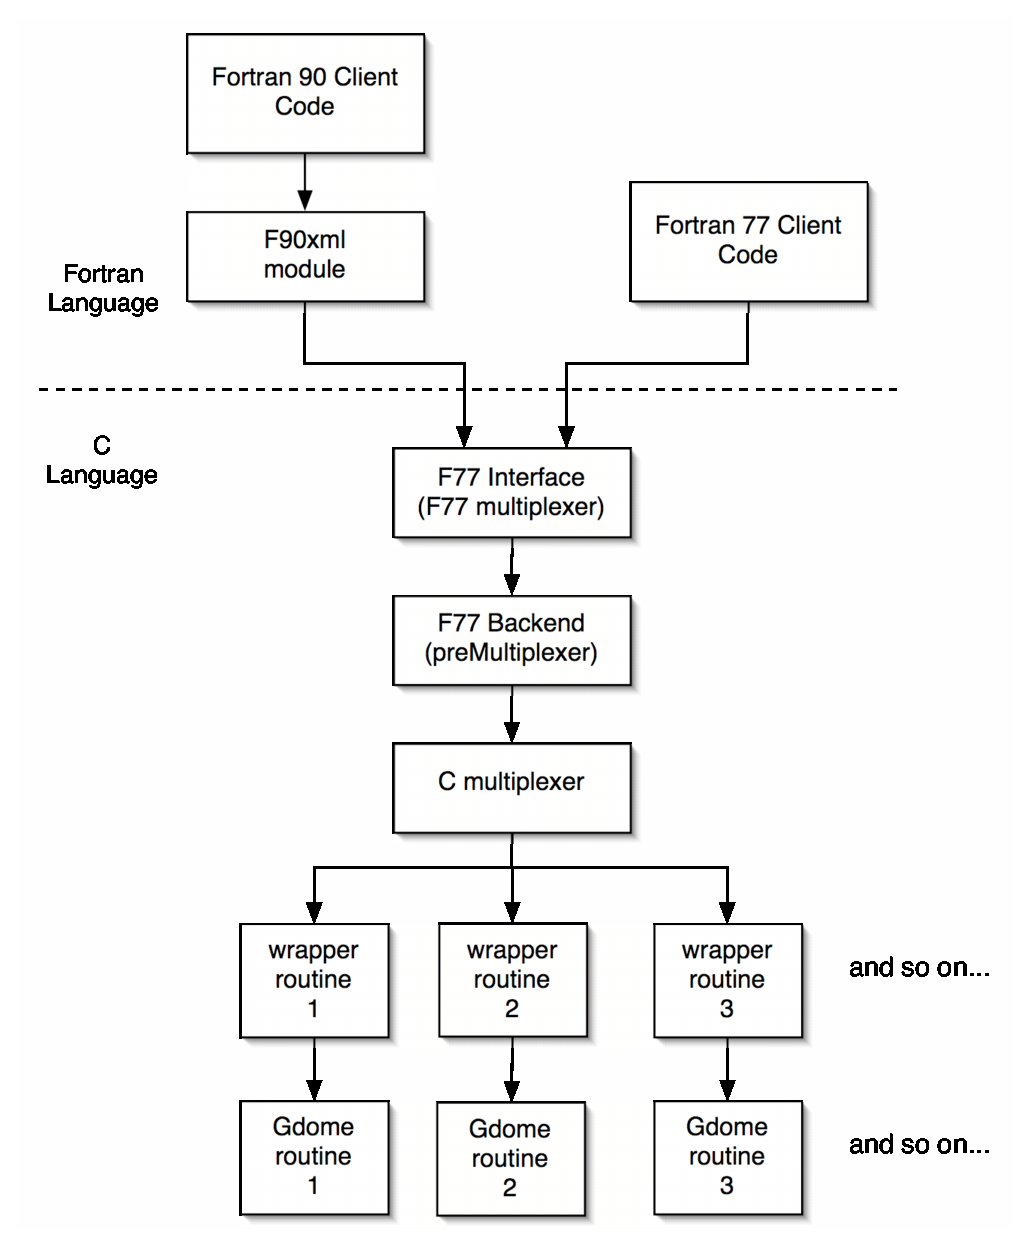
\includegraphics[width=100mm,keepaspectratio]{04_grid/images/f77xml-high-level-gimped.eps}
\end{center}
\caption{\footnotesize A graphical scheme representing the F77/F90xml
library structure. Each multiplexer groups a high number of gdome2
subroutines.}
\label{fig:f77xml-high-level}
\end{figure}
\end{center}

{
\footnotesize
\begin{verbatim}
GdomeBoolean gdome_el_hasChildNodes(GdomeElement *self, GdomeException *exc);
\end{verbatim}
}
has signature \texttt{(b|ce)} and is handled by a multiplexer with the same
\texttt{p} value but different \texttt{t} value: \texttt{xp3t4}

An exception is represented by routines returning \texttt{void},
\texttt{(v|ce)}. These routines are handled as \texttt{(c|ce)} routines,
accepting a dummy return argument which is set to the special value
\texttt{NullCode}. In other terms, both \texttt{(c|ce)} and \texttt{(v|ce)}
routines are managed by the same multiplexer, the \texttt{xp3t1} multiplexer.
It must be pointed out that no matching scheme exists to obtain the type
number from the letter sequence in the signature. 

The \texttt{xp3t1} multiplexer by itself maps and gives access to
approximatively 240 gdome2 functions. The complete DOM interface (more than
450 functions) is mapped by 21 multiplexers. As already said, the
gdome routine is chosen by the means of a \texttt{CHARACTER} argument which
is passed to the multiplexer.  By convention, this argument is passed
between the return value and the first \texttt{INTENT(IN)} argument,
therefore always in the second position. 

As a final result, the Fortran 77 interface to the multiplexer is
represented in the example below

{
\footnotesize
\begin{verbatim}
       CHARACTER*128 fnName
       INTEGER first, last , elem, err

Comment <... get elem by some other call ...>

       fnName='el_firstChild'
       CALL xp3t1(first,fnName,elem,err)

       fnName='el_lastChild'
       CALL xp3t1(last,fnName,elem,err)
\end{verbatim}
}
As can be seen from the example, the function name is case sensitive and is
the exact copy of the gdome2 function, stripped of the ``\texttt{gdome\_}''
prefix.  The Fortran 90 module provides long named subroutines performing
the mapping between each subroutine and the corresponding multiplexer.

The library architecture here presented was chosen for two reasons: 
\begin{itemize}
\item reduce the development cost, providing automatized creation of the
library
\item keep potential Fortran 77 compatibility.
\end{itemize}

A large part of the library is developed in XML. An XML file contains all
the informations to create the binding routines called from the C
multiplexers.  The file is parsed by a Python script which
collects the needed informations, and deploys the C and Fortran code. 

The logic involved is to define templates for the binding routines, and to
replace ad-hoc placeholder keywords with appropriate entries for the
specific routine. When a particular specific implementation cannot be
generated by a template, the format allows to override the template
mechanism and to pass the specific implementation.

We can note that the Fortran 77 interface is a direct subproduct of the
internal implementation of the library, therefore is convenient to deploy it
even if not used by client code. 

%In order to simplify the cleanup of the allocated structures, the
%\textt{f90xml_cache_flush} routine is provided. Using this routine the
%client code can delay the cleanup of many objects to a single final call.
%Functions for unreferencing single structures (Nodes, DOMStrings etc...) are
%also available at F77/F90xml level.
%
%{
%\footnotesize
%\begin{verbatim}
%CHARACTER(LEN=4) :: fortranString
%\end{verbatim}
%}
%
%and accessing the \texttt{f90xml\_str\_toFortran} routine with fortranString and
%offset 0, fortranString will contain "Here" and the returned logical value will
%be \texttt{.FALSE.}. With an offset of 5, fortranString will contain "is t", and
%again the returned logical value will be \texttt{.FALSE.}. Finally, with an offset
%of 13, fortranString will contain "ata" and the returned logical value will
%be \texttt{.TRUE.}. 
%{
%\footnotesize
%\begin{verbatim}
%0 : ERR_NO_ERROR 
%\end{verbatim}
%}
%
%
%{
%\footnotesize
%\begin{verbatim}
%10 : ERR_DATA_NOT_AN_ELEMENT 
%11 : ERR_DATA_NOT_A_NODE  
%12 : ERR_DATA_NOT_A_DOCUMENT 
%13 : ERR_DATA_NOT_A_STRING  
%14 : ERR_DATA_NOT_A_NODELIST 
%15 : ERR_DATA_NOT_A_COMMENT  
%16 : ERR_DATA_NOT_AN_ATTR 
%17 : ERR_DATA_NOT_A_NAMEDNODEMAP 
%18 : ERR_DATA_NOT_A_TEXT     
%19 : ERR_DATA_NOT_AN_ENTITYREF  
%20 : ERR_DATA_NOT_AN_ENTITY 
%21 : ERR_DATA_NOT_A_PROCESSINGINSTRUCTION  
%22 : ERR_DATA_NOT_A_CDATASECTION 
%23 : ERR_DATA_NOT_A_DOCUMENTFRAGMENT
%24 : ERR_DATA_NOT_A_DOCUMENTTYPE   
%25 : ERR_DATA_NOT_A_DOMIMPLEMENTATION  
%\end{verbatim}
%}
%
%These errors are returned every time a passed code is not of the expected type, after inquiry into the cache.
%For example passing the code that corresponds to a DOMImplementation to
%f90xml\_el\_firstChild, a ERR\_DATA\_NOT\_AN\_ELEMENT is returned, because f90xml\_el\_firstChild expects an element.
%It is important to note that a code referring to an Element can be passed to Node handling
%subroutines like f90xml\_n\_appendChild (which accept a code for a node),
%because in the DOM abstraction an Element is a specialization of a Node.
%
%{
%%\footnotesize
%\begin{verbatim}
%30 : ERR_NO_CACHE_HIT
%\end{verbatim}
%}
%
%This error is returned when a given code does not reference to any object in
%the cache. This usually is indicative of a bug in the client code.
%
%{
%\footnotesize
%\begin{verbatim}
%31 : ERR_NULL_CODE
%\end{verbatim}
%}
%
%This error is returned when a NullCode is passed to a routine unable to
%handle it.
%
%{
%\footnotesize
%\begin{verbatim}
%1000 : ERR_NEVER_RETURN_THIS
%\end{verbatim}
%}
%
%A watchdog error value. No routine should return this error. If this
%happens, a library bug is the cause.
%
%{
%\footnotesize
%\begin{verbatim}
%10000: ERR_GDOME
%\end{verbatim}
%}
%
%An error at gdome2 level has been detected. A F77/F90xml library bug can
%trigger this error.



\clearpage
\pagestyle{empty}{\ }\\
\clearpage
\addcontentsline{toc}{chapter}{Conclusions}
\thispagestyle{empty}
{ \Huge \textbf{Conclusions} } 
\vspace{1mm} \\

This work surveyed two innovative techniques dedicated to the
\textit{ab initio} study of molecular systems.

The localization technique makes use of an optimization procedure that
preserves the locality of a starting guess.  An extension of this technique,
named Freeze-and-Cut, allows the reduction of the computational cost by
performing a neglection of those parts of the molecular system not involved
in the phenomenon under study. The localized molecular orbitals are
frozen at a lower level of theory (SCF in this case) to keep into account
their effect. The remaining orbitals are projected onto a subset of the
original basis set, allowing a reduced AO/MO two-electron integrals
transformation. 

The method proved its efficiency on two molecular system: the aminoacid
zwitterion (7Z)-13 ammoniotridec-7-enoate, specifically designed to
test the response of the method to charge interactions, and the highly
conjugated C$_{13}$ polyenal.  A third test on the acetone plus 6 H$_2$O was
attempted to evaluate excited states. In this case, a higher dimensionality
of the basis set is needed to produce effective results, but this attempt
reported a sensivity of the Freeze-and-Cut method to diffuse basis sets. 

A possible solution to this problem is the use of non-orthogonal orbitals between the frozen
and non-frozen sets, and although it seems to produce stable results, the
current procedure have to be reconsidered with the assumption of
non-orthogonality. Further developments are needed to face this
improvement.

The second technique studied during this Ph.D. is the n-Electron Valence
state Perturbation Theory (NEVPT). NEVPT is a multireference perturbation
theory applicable to CAS wavefunctions. It is based on a two-electron
Hamiltonian, the Dyall Hamiltonian, which provides a straightforward and
efficient development for both theoretical and computational implementation.
The perturber wavefunctions are multireference in nature, and belongs to
eight excitation classes, depending on the promotion scheme of the
electrons. 

NEVPT is available in two accuracy levels, depending on the degree of
contraction of the perturber space: the Strongly Contracted NEVPT uses a
monodimensional space for each class, while the Partially Contracted uses a
space of higher dimensionality but smaller than the complete space. The
Strongly Contracted approach produces results of good accuracy when compared
to the Partially Contracted, and a difference between the two approaches has
been noted as a symptom of a poor zero-order wavefunction.

NEVPT is available as a Single-State approach, where the perturbation is
applied to a specified electronic state, and also as a Quasi-Degenerate
approach, where the perturbation effects are applied simultaneously to a set
of states. The Quasi-Degenerate approach keeps into account the
interactions between wavefunctions after the perturbative corrections,
allowing mixing of the states.

Finally, a variation of NEVPT named Non-Canonical has been deployed to
obtain invariability for intraclass orbital rotation for core and virtual
orbitals. This approach removes the need to perform the evaluation on
canonical orbitals, allowing the direct application of NEVPT on a set of
localized orbitals.

The various aspects of NEVPT has been applied to a large set of cases, all
involving the carbonyl system. Every performed evaluation highlighted the
strengths of this method, in particular its computational efficiency, its
accuracy and the absence of intruder states.  In the Quasi-Degenerate NEVPT
further developments can be applied to open the possibility toward an
iterative treatment. An attempt has been successfully made to deploy an
integrated Localized+NEVPT Non-Canonical evaluation. This will open the
possibility to perform highly accurate evaluations on large molecular
systems.

Finally, a collaboration with the CINECA supercomputing center lead to
accurate insights in the problems related to the deployment of a grid
infrastructure for quantum chemistry evaluations. Two problems have been
recognized as rather central in the first phase of the project: the need of
a library for parsing XML with the Fortran language, and a common file
format for large binary data.

The first problem has been addressed with the development of the F90xml library.
This library provides a DOM compliant interface to the Fortran environment,
acting as a wrapper of the gdome2 library.

The second problem involved an accurate analysis of previous common formats
in the field, keeping into account a very large set of new requisites, such
as platform independence, ease of use, debugging accuracy, and
extensibility.  This research lead to the deployment of a data model which
has been implemented in the high-level library Q5Cost. This library proved
its effectiveness allowing various codes to share informations, thus opening
new possibilities in the integration of methods and the development of a
grid metasystem. The library also comes with a proficient testsuite, aimed
at stressing the interface for unexpected error conditions. The result is a
very accurate, extensible and solid library. 

The main drawbacks of this library can be found in the followings: the
envisioned data model at the moment is not completely implemented in the
interface, and the data storage for integrals can be made more efficient in
terms of space occupation. In any case, the current implementation is
optimal for a first-time experimentation in a new panorama for the
computational quantum chemistry, and the detailed informations about the
indexes of the stored integrals can be removed, providing files of reduced
size.

\clearpage
\thispagestyle{empty}
{ \Huge \textbf{Conclusions} } 
\vspace{1mm} \\
\thispagestyle{empty}

Ce travail a regard\'e deux nouvelles techniques pour l'\'etude \textit{ab
initio} des syst\`emes mol\'eculaires. La technique de localisation utilise
une procedure d'optimisation qui preserve la localit\'e d'un groupe
d'orbitales de guess localis\'ee. Une extension de cette technique, la
technique Freeze-and-Cut, permet la r\'eduction du co\^ut computationnel
apr\`es \'elimination de la partie du syst\`eme  mol\'eculaire pas
int\'eress\'ee au ph\'enom\`ene \'etudi\'e.
Les orbitales localis\'ees sont gel\'ees \`a un niveau plus bas de th\'eorie
(dans notre cas, une \'evaluation SCF) et leur effect est preserv\'e. 
Pour r\'eduire le poids computationnel pour la transformation des integrales
bielectroniques, les autres orbitales sont project\'ees sur un sous-ensemble
de la bas atomique original. Cette m\'ethode a \'et\'e essay\'e sur deux
syst\`emes mol\'eculaires: le (7Z)-13 ammoniotridec-7-enoate, un aminoacide
construit pour \'evaluer la r\'eponse de la m\'ethode al'interaction de
charge, et le polyenal C13.
Une troisi\`eme \'evaluation a \'et\'e effectu\'e sur l'etat excit\'e $n \rightarrow
\pi^{*}$ de la molecule d'acetone avec 6 molecules d'eau. Dans ce cas, la
dimensionalit\'e plus grande de la bas atomique a d\'emontr\'e une
sensibilit\'e de la m\'ethode Freeze-and-Cut \`a des bases diffuses. Une solution
peut \^etre l'utilise de orbitales non-ortogonaux entre le groupe gel\'e et
non-gel\'e. Cette solution donne des r\'esultats plus corrects, mais la
procedure courant doit \^etre adapt\'ee avec l'assumption de non
orthogonalit\'e, et donc autres d\'eveloppements theoretiques sont
n\'ecessaires.

La deuxi\'eme technique etudi\'ee pendant ce travail de These est la th\'eorie
perturbative ``n-Electron Valence state Perturbation Theory'' (NEVPT). La NEVPT
est une th\'eorie perturbative multir\'ef\'erence qui peut \^etre
appliqu\'ee
\`a des fonction d'onde de type CAS. Le d\'eveloppement theoretique utilise
un Hamiltonien bielectronique, l'Hamiltonien de Dyall, qui donne une
th\'eorie propre et efficiente. Les fonctions perturbatives sont de nature
multir\'ef\'erencielle, et peuvent \^etre classifi\'ee dans huit classes d'excitation,
selon le sch\'ema de promotion des electrons. La NEVPT existe dans
deux versions, la Strongly Contracted et la Partially
contracted, selon le niveau de contraction de l'espace perturbatif. La
Strongly Contracted NEVPT utilise un espace monodimensionnel pour chaque
classe, et la Partially Contracted utilise un espace \`a dimensionalit\'e plus
haute, mais plus petite que l'espace complet des determinants excit\'es.
L'approche Strongly Contracted donne des r\'esultats de bonne qualit\'e si
compar\'ee avec la Partially Contracted. Une diff\'erence entre eux est
normalement un sympt\^ome d'une mauvaise d\'escription \`a l'ordre-zero.

La NEVPT est disponible comme single \'etat, o\'u la perturbation est
appliqu\'ee \`a un particulier \'etat \'electronique. La NEVPT Quasi Degenerate
applique l'effet perturbatif sur un ensemble d'\'etats \`a la fois. Cette
approche consid\`ere les interactions entre les fonctions d'onde apr\`es la
perturbation, et permit le m\'elange de ce fonctions.
Enfin, une variation de la NEVPT appell\'ee Non Canonical a \'et\'e
d\'evelopp\'ee pour obtenir l'invariabilit\'e des r\'esultats pour le
m\'elange des orbitales de core et virtuelles. Cette approche \'elimine la
n\'ecessit\'e de travailler avec des orbitales canoniques, et permit
l'utilisation directe avec un ensemble d'orbitales localis\'ees.

Les diff\'erents types de NEVPT ont \'et\'e utilis\'es sur un ensemble de
syst\'emes concernant le group carbonyl. Toutes les \'evaluations effectu\'ees
donnent des r\'esultats int\'eressants, et sont aussi inter\'essantes les
propri\'et\'es de la NEVPT, comme l'efficacit\'e computationnelle et l'absence
d'\'etats intrus.
Les r\'esultats de la th\'eorie QD-NEVPT peuvent \^etre amelior\'ees avec une
procedure iterative, qui peut \^etre une bonne solution \`a des
probl\'emes dans les r\'esultats obtenus.
L'integration de la th\'eorie NEVPT avec l'approche localis\'ee a \'et\'e
effectu\'ee avec la NEVPT Non Canonique. Cette travail sera important pour
effectuer des calculs sur syst\'emes mol\'eculaires de grande taille.

Une collaboration avec le centre de supercalcul CINECA a \'et\'e aussi
effectu\'ee dans le cadre d'un projet international entre diff\'erent
instituts de recherche en chimie quantique. L'objectif est l'integration des 
diff\'erentes m\'ethodologies \textit{ab initio} dans une r\'eseau d'ordinateurs.
Deux probl\`emes sont prioritaires dans la phase initial du projet: la
n\'ecessit\'e d'une bibliotheque pour la lecture du format de fichier XML avec
le langage Fortran, et le d\'eveloppement d'un format de fichier binaire
commun pour le stockage de donnees de grand taille.
Pour le premier probl\`eme, la biblioth\`eque F90xml a \'et\'e
d\'evelopp\'ee. Cette biblioth\`eque interface libgdome2 (biblioth\`eque
pour le langage C) avec Fortran. 

Pour le deuxi\`eme probl\`eme, on a analis\'e le format de fichier dej\`a
d\'evelopp\'e et evalu\'e leur d\'efects pour l'ex\'ecution en grid, qui
n\'ecessite de consid\'erations additionnelles, comme
ind\'ependance de plateforme, simplicit\'e d'utilise de la biblioth\`eque 
d'acces, exactitude des messages d'erreur et extensibilit\'e.
La recherche effectu\'ee a conduit au d\'eveloppement d'un mod\`ele des
donn\'ees qui a \'et\'e impl\'ement\'e dans la biblioth\`eque Q5Cost. Cette
biblioth\`eque a \'et\'e utilis\'ee pour l'integration des diff\'erents logiciels,
et ouvre des nouvelles possibilit\'es pour le partage d'information
quantistique et l'integration des m\'ethodes \textit{ab initio}.
La biblioth\`eque a aussi une testsuite pour contr\^oler l'interface et
chercher les probl\`emes dans l'implementation. 
Le r\'esultat est une biblioth\`eque tr\`es solide et extensible.  Le
probl\`emes principaux qui restent \`a resoudre dans Q5Cost sont: le
stockage des integrals n'est pas encore efficient en terms d'espace
occup\'e, et l'implementation du mod\`ele des donn\'ees n'est pas complete,
mais l'impl\'ementation courante est suffisante pour le premiers
d\'eveloppements et implementations.

\clearpage
\pagestyle{fancy}
\clearpage
\addcontentsline{toc}{chapter}{Bibliography}
%\nocite{*}
\bibliographystyle{acs}
\bibliography{thesis}

\end{document}



